\immediate\write18{makeindex \jobname.nlo -s nomencl.ist -o \jobname.nls}
%\documentclass[showtrims,oldfontcommands]{kthesis}
\documentclass[g5paper,phd,electronic]{preamble/kthesis}
% \documentclass[oldfontcommands]{kthesis}
\usepackage[bookmarks]{hyperref}
\usepackage[T1]{fontenc}
\usepackage{textcomp}
\usepackage{lmodern}
\usepackage[utf8]{inputenc}
\usepackage[swedish,english]{babel}
\usepackage{amsmath,amssymb}
\usepackage{graphicx,psfrag}
\usepackage{color}
\usepackage{cite}
\usepackage{url}
\usepackage{array}
\usepackage{enumerate}
\usepackage{amsthm}
\usepackage{comment}
\usepackage{float}
\usepackage{algorithm}
\usepackage{algorithmic}
\usepackage{balance}
\usepackage{bm}
% \usepackage{subfig}
\usepackage{epstopdf}
\usepackage{comment}
\usepackage{makeidx}
% Several biblographies
\usepackage{bibunits}
% figure drawing
\usepackage{tikz}
\usetikzlibrary{calc,shapes,positioning}
\usetikzlibrary{arrows}
\usetikzlibrary{fit}
\newcommand{\midarrow}{\tikz \draw[-triangle 90] (0,0) -- +(.1,0);}
% set arrow type and size by tikz
% alternative to 'Straight Barb' can be 'Latex, Stealth, Computer Modern Rightarrow'.
\usetikzlibrary{arrows.meta}
\tikzset{>={Straight Barb[width=1.3mm,length=1.3mm]}}
\usepackage{adjustbox}

\makeindex
% allow subfigure environment
\usepackage{subcaption}

\usepackage{nomencl}
\makenomenclature
\renewcommand{\nomname}{Acronyms and Notations}
\usepackage{etoolbox}
\renewcommand\nomgroup[1]{
\item[\bfseries
\ifstrequal{#1}{A}{Acronyms}{%
\ifstrequal{#1}{N}{Notations}{}}
]}

\usepackage{rotating}
\usepackage{preamble/mystyle}
\setlength{\textfloatsep}{5pt}
\maxsecnumdepth{subsection}
\setsecnumdepth{subsection}
% indent the first paragraph
\usepackage{indentfirst}



%%% Local Variables:
%%% mode: latex
%%% TeX-master: "../main"
%%% End:

\title{Perspectives on Probabilistic Graphical Models}
%\subtitle{}
\author{Dong Liu}
\date{2020}
\thesistype{Doctoral Thesis in Electrical Engineering}
\imprint{Stockholm, Sweden 2020}
\examen{teknologie doktorsexamen i Elektroteknik}
\disputationsdatum{måndag den 16 Noviembre 2020 klockan 13:30}
\disputationslokal{F3, Lindstedtsv\"{a}gen 26, Stockholm}
\isbn{ISBN 978-91-7873-671-3}
% \issn{ISSN ....}
%\isrn{}
\trita{TRITA-EECS-AVL-2020:55}
\publisher{Universitetsservice US AB}
\address{KTH Royal Institute of Technology\\
  School of Electrical Engineering and Computer Science\\
  Department of Intelligent Systems\\
  Information Science and Engineering\\
  SE-100 44 Stockholm\\
  SWEDEN}
\kthlogo{logo/kthlogo}
\endinput

%%% Local Variables:
%%% mode: latex
%%% TeX-master: "main"
%%% End:


\begin{document}

\frontmatter
\maketitle
\thispagestyle{empty}
\vfill
\begin{figure}
\begin{flushright}
\Large
\textit{To my mother\\
In loving memory of my father}
\end{flushright}
\end{figure}
\vfill

% abstract
\chapter{Abstract}
Probabilistic graphical models provide a natural framework for representation of complex systems and offer straightforward abstraction for the interactions within the systems. Reasoning with probabilistic graphical models allows us to answer inference queries with uncertainty following the framework of probabilistic theory. General inference queries include the computation of marginal probabilities or conditional probabilities of states of a system, or evaluation of the partition function of the underlining distribution of a Markov random field (undirected graphical model). Critically, the success of graphical models in practice largely relies on efficient approximate inference methods that offer fast and accurate reasoning results. Closely related to the inference tasks in graphical models, another fundamental problem is to decide the parameters of a candidate graphical model by extracting information of empirical observations, i.e., parameter learning of a graphical model. The two essential topics (i.e., inference and learning) interacts with and facilitate each other. For instance, learning of a graphical model usually uses a inference method as a subroutine while the learned graphical model is then employed for inference tasks in presence of new evidence.

In this dissertation, we develop new algorithms and models for generic inference in Markov random fields. We firstly present an alternative view of belief propagation in term of a divergence minimization, which is in contract to the view of free energy minimization. The alternative view brings the development of a variant algorithm of belief propagation that turns out generalizes standard belief propagation algorithm. Insights on the convergence behaviors of the developed algorithm in the binary state space are provided apart from the intuition in development. As a step beyond approximate inference with message passing, we develop a region-based energy network model that performs generic inference via region-based free energy minimization, which turns inference in Markov random fields into a optimization problem. This model incorporates both our essential understanding of inference and modern computational efficiency of modern neural network models.

The further part of the dissertation focus on the parameter learning of probabilistic graphical models. This part starts with the discussion on parameter learning of undirected graphical models and explain the role of an (approximate) inference method in this routine. As directed graphical models, new finite mixture models incorporating normalizing flows in neural network implementations are presented for more expressive and flexible modeling. The learning of developed generic models is handled within expectation maximization due to the presence of hidden (or latent) variables. The expressive modeling method and learning are further extended into dynamic systems within a reduced dynamic Bayesian network, i.e., a hidden Markov model. The dissertation closes with a chapter on the likelihood-free learning of a class of directed graphical models, where (directed) generative models induce implicit probabilistic distributions and are learned by the optimal transport distance.


%%% Local Variables:
%%% mode: latex
%%% TeX-master: "../main"
%%% End:

% \clearpage

\chapter{Sammanfattning}

\begin{otherlanguage}{swedish}
Probabilistiska grafiska modeller utgör ett naturligt ramverk för representation av komplexa system och erbjuder enkel abstraktion av interaktioner inom systemen.
Resonemang baserade på probabilistiska grafiska modeller tillåter oss att genomföra statistisk slutledning (inferens) med osäkerhet inom ramarna för probabilistisk teori. Allmän statistisk inferens innefattar beräkning av marginella eller betingade sannolikheter för olika tillstånd i ett system, eller utvärdering av partitionsfunktionen för den underliggande fördelningen i ett slumpmässigt Markov fält (icke-riktad grafisk modell). Fördelarna med grafiska modeller beror i praktiken till stor del på tillgången till effektiva approximativa inferensmetoder som tillhandahåller snabba och träffsäkra resultat. Ett annat grundläggande problem, nära besläktat med den inferens som utförs i grafiska modeller, är att bestämma parametrarna för en grafisk kandidatmodell genom att extrahera information från empiriska observationer, d.v.s. inlärning av parametrar för en grafisk modell. Dessa två centrala uppgifter (dvs. slutledning och inlärning) både interagerar med, och underlättar för, varandra. Till exempel innefattar inlärning av en grafisk modell vanligtvis en inferensmetod som en subrutin medan den inlärda grafiska modellen sedan används för inferensproblem baserade på ny data.

I denna avhandling utvecklar vi nya algoritmer och modeller för generisk inferens i slumpmässiga Markov-fält. Inledningsvis presenterar vi en alternativ metod för sannolikhetspropagering (s.k. "belief propagation") genom minimering av divergens, vilket står i motsats till metoder baserade på minimering av fri energi. Detta alternativa tillvägagångssätt leder till utveckling av en ny typ av algoritm för sannolikhetspropagering som visar sig utgöra en generalisering av standardalgoritmen. Insikter om konvergensbeteendet hos den utvecklade algoritmen i det binära fallet tillhandahålls bortsett från intuitionen under utveckling. Som ett ytterligare steg utöver approximativ inferens baserad på s.k. "message passing" utvecklar vi en regionsbaserad energi-nätverksmodell som utför generisk inferens via regionsbaserad  minimering av fri energi. Detta transformerar slutledningsproblemet i slumpmässiga Markov-fält till ett optimeringsproblem. Denna modell innefattar vår väsentliga förståelse för både inferens och beräkningseffektivitet hos moderna neurala nätverksmodeller.

Nästa del av avhandlingen fokuserar på parameterinlärning av probabilistiska grafiska modeller. Denna del inleds med en diskussion om parameterinlärning av icke-riktade grafiska modeller samt förklarar en (approximativ) inferensmetods roll inom denna rutin. För riktade grafiska modeller presenteras nya ändliga "mixture"-modeller som inkluderar normaliseringsflöden i neurala nätverksimplementeringar för mer träffsäker och flexibel modellering. Inlärningen av de utvecklade generiska modellerna hanteras av s.k "expectation maximization" på grund av närvaron av dolda (eller latenta) variabler. Den träffsäkra modelleringsmetoden och inlärningen utvidgas ytterligare till dynamiska system inom ett reducerat dynamiskt Bayesian-nätverk, dvs en dold Markov-modell. Avhandlingen avslutas med ett kapitel om sannolikhetsfri inlärning av en viss klass av riktade grafiska modeller, där (riktade) generativa modeller genererar implicita sannolikhetsfördelningar och tränas via det optimala transportavståndet.
\end{otherlanguage}

%%% Local Variables:
%%% mode: latex
%%% TeX-master: "../main"
%%% End:

% \clearpage

\chapter{Acknowledgements}
This Ph.D. journey would not be possible without these people to be acknowledged here.

First and foremost, I would like to express my deep gratitude towards my supervisor Prof. Lars K. Rasmussen. At the beginning of this journey, Lars remarked to me, 'Let us do something interesting'. This code revealed more power later as time went than it sounded at the beginning. In the long and challenging journey, it was the propulsion from interests that drove me all the way here. At the time that I lay these words to my thesis, I still feel the joy of doing what I do in research. Lars has been always supportive in advising me and teaching me the way to do research, though there were inevitably detours in research journeys. Whenever I was in moments of confusion and frustrations, Lars's positive attitude and humor brought me back to balance.
I would like to thank my supervisor Assoc. Prof. Ragnar Thobaben for his consistent support to me in my education. I benefited from every meeting with him. His comments on my thesis were always insightful input and to the point. The work with Ragnar was efficient and joyful. I was lucky to have Lars and Ragnar as my advisors on this journey.

I am grateful to Assoc. Prof. Saikat Chatterjee and Dr. Minh Th\`{a}nh Vu. There are always interesting ideas from Saikat's active mind. Fortunately, our offices are just several steps away, which allows quick discussions before the inspiration fades out. Thank you, Saikat, for the sacrifice of weekends and holidays to help me with improving my drafts.
I own the thanks to Minh for conveying many prohibitive problems in intuitive ways in our discussions, which gradually helped to form my own way of comprehending complex issues. I am impressed by how knowledgeable this mind is and how fast the mind processes problems. I learned a lot from him. I would like to express my sincere gratitude to Minh for the consistent guidance of my research.

I am indebted to Prof. Viktoria Fodor and Assoc. Prof. Chao Wang who shared valuable research experiences, were helpful and supportive in collaborations. I am fortunate to have had joint work with Antoine Honor{\'e}, Baptiste Cavarec, Dr. Jing Yue, Dr. Jinliang Huang, Dr. Zuxing Li, and Dr. Nima N. Moghadam. I have benefited tremendously from interactions with them.

I would like to thank both Dr. Pol Del Aguila Pla and Xuechun Xu for their quick responses to my frequent requests for packages and dependencies on the computational servers. I thank Sina Molavipour for being my teaching partner. I would also like to thank Henrik Forssell for the help with the Swedish abstract.


I am fortunate to have fantastic colleagues at ISE. I really enjoyed the badminton activities with Alireza Mahdavi Javid, Ramana Reddy Avula, Xuechun, Zuxing, and Saikat. The relaxed time of lunches and fikas with Shaocheng Huang, Dr. Yu Ye, Boules Atef Mouris, Sahar Imtiaz, Dr. Guang Yang, Dr. Le Phuong Cao, Dr. Marie Maros, Dr. Germ\'{a}n Bassi, and Dr. Arun Venkitaraman were pleasant in office kitchens.

I am always grateful to my master study adviser Prof. Erwu Liu in Tongji for encouraging me to do Ph.D. research. This journey is challenging and fruitful.

I cannot thank enough to my mother, Zirong Li, who has never stopped encouraging me to pursue what I want, and has always been there for me, being supportive. \newline
\newline


\hfill
Dong Liu

\hfill
Stockholm, August 2020





%%% Local Variables:
%%% mode: latex
%%% TeX-master: "../main"
%%% End:

\clearpage

\tableofcontents
% \cleardoublepage

% 
% \nomenclature[A]{}{}
% \nomenclature[A]{CPS}{cyber-physical system}
% \nomenclature[A]{i.i.d.}{identically independently distributed}
% \nomenclature[A]{LRT}{likelihood-ratio test}
% \nomenclature[A]{p.d.f.}{probability density function}
% \nomenclature[A]{p.m.f.}{probability mass function}
% \nomenclature[A]{ROC}{receiver operating characteristic}
% \nomenclature[A]{PBPO}{person-by-person optimization}
% \nomenclature[A]{FC}{fusion center}
% \nomenclature[A]{EVE}{eavesdropper}
% \nomenclature[A]{AD}{adversary}
% \nomenclature[A]{EP}{energy provider}
% \nomenclature[A]{RES}{renewable energy source}
% \nomenclature[A]{EMU}{energy management unit}
% \nomenclature[A]{ES}{energy storage}
% \nomenclature[A]{GDPR}{General Data Protection Regulation}
% \nomenclature[A]{KKT}{Karush-Kuhn-Tucker}
% \nomenclature[A]{LRC}{likelihood-ratio chain}
% \nomenclature[A]{MDP}{Markov decision process}

%\nomenclature[N]{}{}
\nomenclature[N,11]{$X$}{random variable}
\nomenclature[N,12]{$x$}{realization of the random variable $X$}
\nomenclature[N,13]{$\mathcal{X}$}{alphabet of the random variable $X$}
\nomenclature[N,21]{$X_{i}^{k}$}{random sequence $(X_{i},\dots,X_{k})$}
\nomenclature[N,22]{$x_{i}^{k}$}{realization of the random sequence $X_{i}^{k}$}
\nomenclature[N,23]{$\mathcal{X}_{i}^{k}$}{alphabet of the random sequence $X_{i}^{k}$}
\nomenclature[N,31]{$X^{k}$}{random sequence $(X_{1},\dots,X_{k})$}
\nomenclature[N,32]{$x^{k}$}{realization of the random sequence $X^{k}$}
\nomenclature[N,33]{$\mathcal{X}^{k}$}{alphabet of the random sequence $X^{k}$}
\nomenclature[N,41]{$X_{i}^{k\setminus n}$}{random sequence $(X_{i},\dots,X_{n-1},X_{n+1},\dots,X_{k})$}
\nomenclature[N,42]{$x_{i}^{k\setminus n}$}{realization of the random sequence $X_{i}^{k\setminus n}$}
\nomenclature[N,43]{$\mathcal{X}_{i}^{k\setminus n}$}{alphabet of the random sequence $X_{i}^{k\setminus n}$}
\nomenclature[N,51]{$X^{k\setminus n}$}{random sequence $(X_{1},\dots,X_{n-1},X_{n+1},\dots,X_{k})$}
\nomenclature[N,52]{$x^{k\setminus n}$}{realization of the random sequence $X^{k\setminus n}$}
\nomenclature[N,53]{$\mathcal{X}^{k\setminus n}$}{alphabet of the random sequence $X^{k\setminus n}$}
\nomenclature[N,61]{$\vert\vert\cdot\vert\vert$}{set cardinality}
\nomenclature[N,62]{$f_{X}$}{p.d.f. of the continuous random variable $X$}
\nomenclature[N,63]{$p_{X}$}{p.m.f. of the discrete random variable $X$}
\nomenclature[N,64]{$\mathcal{N}(\mu,\sigma^{2})$}{normal distribution with mean $\mu$ and variance $\sigma^{2}$}
\nomenclature[N,71]{$\textnormal{D}(\cdot\vert\vert\cdot)$}{Kullback-Leibler divergence}
\nomenclature[N,72]{$\textnormal{D}_{\tau}(\cdot\vert\vert\cdot)$}{$\tau$-th order R\'{e}nyi divergence}
\nomenclature[N,73]{$\textnormal{C}(\cdot,\cdot)$}{Chernoff information}
\nomenclature[N,81]{$\textnormal{E}[\cdot]$}{expectation}
\nomenclature[N,91]{$\partial\cdot$}{boundary of a closed set}
\nomenclature[N,92]{$\hat\partial\cdot$}{upper boundary of a two-dimensional closed set}
\nomenclature[N,93]{$\check\partial\cdot$}{lower boundary of a two-dimensional closed set}
\nomenclature[N,94]{$\log(\cdot)$}{natural logarithm}
\addcontentsline{toc}{chapter}{Acronyms and Notations}
\markboth{ACRONYMS AND NOTATIONS}{ACRONYMS AND NOTATIONS}
\printnomenclature[2cm]

%%% Local Variables:
%%% mode: latex
%%% TeX-master: "../main"
%%% End:

\mainmatter

% Beginning of main content: chapter 1
\chapter{Introduction}
\label{chapter1}

\section{Motivations}
\label{section1.1}

Most tasks conducted by a person or an automated system requires a fundamental ability of \textit{reasoning}, which is always about reaching a conclusion based on available information. At times, a conclusion is not enough and it is also required to know how reliable the conclusion is. Take the coronavirus (COVID-19) that started from Wuhan in China at the end of 2019 as example, a doctor needs to check the information about a person to reason if the person is infected by the coronavirus. The relevant information includes symptoms such as fever, cough, breathing difficulties and probably kidney failure in severe cases. Even after the doctor has reached a conclusion of positive or negative infection of coronavirus for the person, a natural question is why and how \textit{confident} the diagnose is made.

Instead of randomly guessing, reasoning is to answer queries with preserving uncertainty, by making best of available information. Two fundamental problems are inevitable before a rational reasoning can be conducted. 
\begin{itemize}
\item How should we specify the relationship between a conclusion and the available information? In the coronavirus example, the counterpart question to answer is how the doctor should relate coronavirus infection with the symptoms. This step is called \textit{modeling} which represents a reasoning problem abstractly by specifying the relationship between known information and unknown parts, in preparation of answer query on it.
\item With the modeled representation, how a conclusion should be made? This process of reaching a answer to the query from an abstracted representation is called \textit{inference}. Assume the doctor knows that the candidate has fever and cough, but not any breathing problem, how likely does the candidate have be infected by coronavirus?
\end{itemize}

In the modeling and inference process, it is not likely that the very beginning assumptions are perfectly right about the truth and can be used for all instances of the same type of queries. On the contrary, we usually begin with simple (sometimes naive) assumptions of representation a problem, and come back to revise it later when more information or evidence is available, which is aligned with our learning process of new knowledge. In fact, this assumption-and-revision procedure can be more compact. Instead of fixing the model representation at the beginning when one might not be sure the correctness of the assumptions about the model, one can assume a set of models with the assumption that the 'correct' model is in this set. A typical strategy is to leave some freedom to the configuration of the model at the beginning. Each instantiating the configuration generates a model representation. By using available observations or information, the model is adjusted to be able to be best compatible with the observations. This procedure adds the following fundamental problem in reasoning.
\begin{itemize}
\item Instead of having a fixed model at the first step, a set of models (or hypothesis) is given. We then need to choose one model that best describes the available observations or information. This phase of choosing a model is called \textit{learning}. 
\end{itemize}
Afterwards, inference can be conducted on the learned model to answer queries.

With all the discussed problems above, modeling, inference and learning, our purpose is to carry out reasoning with being aware of how confident a conclusion or answer is. 
These problems can be treated nicely with probabilistic models via Bayesian logic. Probabilistic model is built on the fundamental calculus of probability theory that is natural to accommodate the \textit{uncertainty}, which is desired in reasoning. In additional, the probabilistic models offers rich space to modeling problems, where inference can be carried on either exactly or approximately. \textbf{More importantly, the modeling or modeling learning part is not necessarily coupled with inference algorithms}. This proper separation allows freedom that a certain family of general inference algorithms can be applies to a broad class probabilistic models. It offers the freedom of trying different model representation of a class without the need of replacing inference algorithm. 

\begin{example}\label{example-corona}
  Consider the coronavirus infection problem. Using probabilistic model, we are able to model the problem in a rigid way. Additionally, we can make query more formally in probabilistic model framework. Assume each symptom among fever, cough and breathing difficulty can take value from $\left\{ \mathrm{True}, \mathrm{False} \right\}$. Also the coronavirus infection is either true or false. One exemplified query can be
  \begin{equation}
    P(\mathrm{Infection} = \mathrm{True} | \mathrm{Fever} = \mathrm{True}, \mathrm{Cough} = \mathrm{False}, \mathrm{Breathing Difficulty}= \mathrm{True}), \nonumber
  \end{equation}
  which is asking how likely the patient is infected by coronavirus if symptoms of both fever and breathing difficulty are observed but no sight of cough symptom.

\end{example}

\begin{figure}[!t]
  % \captionsetup[subfigure]{justification=centering}
  \begin{subfigure}{.4\textwidth}
    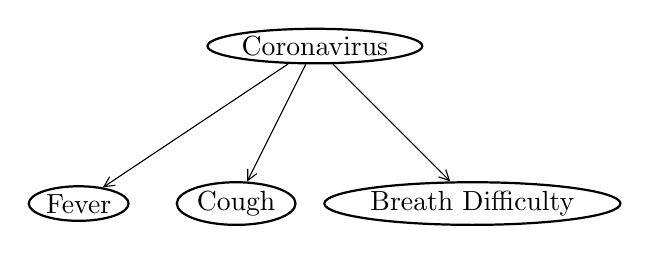
\begin{tikzpicture}
      \tikzstyle{cnode} = [thick, draw=black, ellipse, inner sep = 1pt,  align=center]
      \tikzstyle{nnode} = [thick, rectangle, rounded corners = 0pt,draw,inner sep = 2pt]
      \node[cnode] (virus) at (0,-1) {Coronavirus};
      \node[cnode] (fever) at (-3,-3) {Fever};
      \node[cnode] (cough) at (-1,-3) {Cough};
      \node[cnode] (breath) at (2, -3) {Breath Difficulty};
      \draw[->] (virus) -- (fever);
      \draw[->] (virus) -- (cough);
      \draw[->] (virus) -- (breath);
    \end{tikzpicture}
    \caption{A directed graphical model for Example~\ref{example-corona}.}
    \label{fig:dag-coronavirus}
  \end{subfigure}\hspace{2.5cm}
  \begin{subfigure}{0.3\textwidth}
    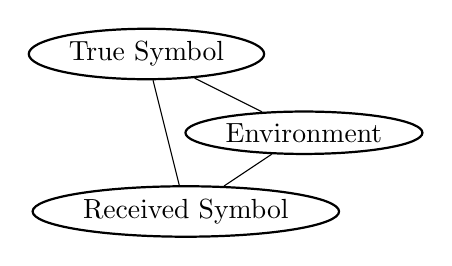
\begin{tikzpicture}
      \tikzstyle{cnode} = [thick, draw=black, ellipse, inner sep = 2pt,  align=center]
      \node[cnode] (ts) at (0,0) {True Symbol};
      \node[cnode] (rs) at (0.5,-2) {Received Symbol};
      \node[cnode] (env) at (2,-1) {Environment};
      
      \draw[-] (ts) -- (rs);
      \draw[-] (ts) -- (env);
      \draw[-] (rs) -- (env);
      
    \end{tikzpicture}
    \caption{An undirected graphical model.}
    \label{fig:mrf-communication}
  \end{subfigure}
  \caption{Different perspectives on probabilistic graphic models. \ref{fig:dag-coronavirus} A toy Bayesian network. \ref{fig:mrf-communication} A toy Markov random field.}
  \hspace{1cm}
\end{figure}


Given the fact that probabilistic theory offers a rigid foundation to model and study the problems, which is used to answer query that we concern, it soon becomes intractable when dozens or hundreds of relevant attributes are joint considered. This can be exemplified by giving finer levels of each symptom in coronavirus infection, e.g. symptom fever is represented by the actual body temperature in integer instead of true-or-false binary state on the one hand. On the other hand, there could be more directly and indirectly relevant symptoms such as muscle pain and congestion. Together with the symptoms, the recent travel itinerary is also related. Additionally, season flu could also similarly bring up some symptoms listed above. 

Probabilistic graphical model offers a general framework to encode random variable dependency of a complex probabilistic distribution into a structured graph, which is a powerful tool to compactly model relevant attributes and facts of a complex problem or a system. As show in Figure~\ref{fig:dag-coronavirus} that represents the problem of Example~\ref{example-corona} into a directed graphical model (also called Bayesian network or generative model), the nodes (or vertexes) correspond to the variables that represents symptoms and infection state, whereas the edges between nodes correspond how one variable may influence others. In certain scenarios, it is natural to use directed graphical models (generative models) to represent that a observable variable is dependent on a latent variable that generates the observations. For instance, a noisy location sensor of a car keeps measuring the car's true location and reading noisy locations. 

In contract to the directed graphical model, there are more scenarios that the interaction between related random variables is not directional and an undirected edge is used, which leads to the undirected graphical model (or Markov random field, Section~\ref{chpt2:sec:graphical-models}) representation. Undirected graphical models are popularly used in computer vision, computational biology, digital communication, statistical physics, etc. Figure~\ref{fig:mrf-communication} illustrates an exemplified undirected graphical model in digital communication context. On the one hand, a receiver wants to know what is the true symbol by joint considering its communication environment and its received symbol. On the other hand, the symbol received by the receiver is jointly formulated by the true symbol and communication environment. The influence among them is apparently not directional since the impact along an edge can be bidirectional in this example.

Probabilistic graphical model offers a 'scientific language' to do reasoning with uncertainty within framework of probabilistic theory. It is usually a nature representation for a complex system or problem and offers straightforward abstraction. The compact representation of probabilistic graphical model bridges the joint distribution of a complex system, and its graphical abstraction that captures the statistic dependency reflecting our understanding of the system. The advantage of its representation power is one of the reasons that leads to its popularity in difference disciplines.

\begin{figure}[!t]
  \centering
  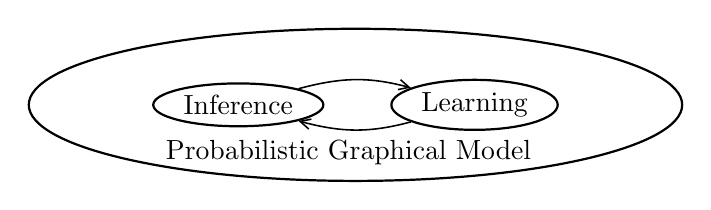
\begin{tikzpicture}
    \tikzstyle{cnode} = [thick, draw=black, ellipse, inner sep = 2pt,  align=center]
    \tikzstyle{fnode} = [thick, draw=black, ellipse, inner sep = 10pt,  align=center]
    
    \node[cnode] (infn) at (0,0) {Inference};
    \node[cnode] (lern) at (3,0) {Learning};
    
    \node[fnode, fit=(infn)(lern)] (box) {};
    \node[] at (1.4, -0.6) {Probabilistic Graphical Model};
    \draw[->,line width=0.2mm] (infn) to[out=15, in=165] (lern);
    \draw[->,line width=0.2mm] (lern) to[out=195, in=-15] (infn);
  \end{tikzpicture}
  \caption{Two key aspects in practical graphical models.}
  \label{fig:intro-pgm}
  \hspace{1cm}
\end{figure}

Probabilistic graphical model coupled with its underlining distribution is a powerful tool for effective inference, apart from its advantage of representation power. It allows to answer queries with the help of the underlining distribution when practical inference algorithms are provided, which meets our need of reasoning with uncertainty. In addition to inference, probabilistic graphical model also supports learning from data. With certain amount of data available, a probabilistic graphical model can be learned to explain the observed data better in addition to align with our own understanding of a domain. The learned graphical model can serve to do inference with higher confidence in return. A diagram is illustrated in Figure~\ref{fig:intro-pgm}. As would become clear in Part~\ref{part:learning}, the inference may be needed to carry out model learning as well, apart from the above mutual-benefiting interaction.



\section{Scope and Thesis Outline}\label{chpt1:sec:scope-outline}
We gives the intuition and motivation of probabilistic graphical model in last section, and the interaction between inference and learning in this framework. In this section, we would navigate further among the topics within this framework and states the ones that we would cover in the thesis.

Inference in probabilistic graphical model is about answering queries with help of its coupled distribution. These queries can be generally grouped into the following cases:
\begin{itemize}
\item Computing the likelihood of observed data or unobserved random variable.
\item Computing the marginals distribution over a particular subset of random variables.
\item Computing the conditional distribution a subset of variables given the configuration of another subset of variables. 
\item Computing the most likely configuration of (a subset of) variables.
\end{itemize}
\textit{The work of this thesis would be mainly related with the first three cases in inference part.}


Due to either the requirement of efficiency in solving a problem or the structure of the problem's graphical model representation, it is not always that case that the above inference problem can solved exactly. Thus inference methods can be divided into
\begin{itemize}
\item exact inference,
\item and approximate inference.
\end{itemize}
For a limited class of graphs, exact inference such as variable elimination and sum-product algorithm can be used. Some graphs also allow efficient inference after mild graph modification, e.g. junction tree method. However, the above listed inference problems can only be approximately solved in general graphs. The approximate inference family can be further divided into
\begin{itemize}
\item Stochastic Approximation (Particle methods),
\item Deterministic Approximation (Variational methods).
\end{itemize}
Stochastic approximation mainly relies on sample instances to answer queries, where a major challenge lies in how to obtain samples efficiently from a target distribution. Gibbs sampling, importance sampling and Markov Chain Monte Carlo are within this family. On the other hand, deterministic approximations refer to the variational methods, such as mean field approximation, loopy belief propagation, expectation propagation etc. \textit{From the perspectives of methodology, we related work in this thesis locates in the family of variational methods under approximate inference category.}


As for learning in probabilistic graphical models, there are two types of learning problems
\begin{itemize}
\item Structure learning,
\item Parameter learning.
\end{itemize}
The first case refer to determine the structure of a graphical model from observations, which is usually reduced to the problem of whether there should be an edge between a pair of nodes in the graphical model. The parameter learning is about to determine the parameter of a probabilistic graphical model (or its coupled distribution), with its graphical structure known. Structure learning is out of the scope of this thesis. The term \textit{learning} in thesis means the estimation of the parameters of a distribution. This problem is mainly discussed in Part~\ref{part:learning}, where we would touch the topics about learning in both undirected and directed graphical models. 


As for the learning techniques, the learning principles can categorized into
\begin{itemize}
\item Maximal likelihood estimation
\item Maximal conditional likelihood
\item Bayesian estimation
\item Maximal `Margin`
\item Maximum entropy
\end{itemize}
in general. We would touch techniques of the first four cases in Part~\ref{part:learning}.

\subsection{Publications}
\textcolor{blue}{Todo: add code repository}

\begin{itemize}
\item Dong Liu and Lars K Rasmussen. Region-based energy nerual network for approximate
inference. Under review, 2020.
\item Dong Liu, Minh Th\`{a}nh Vu, Li Zuxing, and Lars K Rasmussen. $\alpha$ belief propagation for approximate beyeisian inference. Under review, 2020.

\item Dong Liu, Antoine Honor{\'e}, Saikat Chatterjee, and Lars K Rasmussen. Powering hidden
markov model by neural network based generative models. In the 24th European Conference on Artificial Intelligence (ECAI), 2020.

\item Dong Liu, Minh Th\`{a}nh Vu, Saikat Chatterjee, and Lars K Rasmussen. Neural network
based explicit mixture models and expectation-maximization based learning. arXiv preprint
arXiv:1907.13432, 2019.

\item Antoine Honor{\'e}, Dong Liu, David Forsberg, Karen Coste, Eric Herlenius, Saikat Chatterjee, and Mikael Skoglund. Hidden markov models for sepsis detection in preterm infants. In 2020 IEEE International Conference on Acoustics, Speech and Signal Processing (ICASSP),2020.

\item D. Liu, N. N. Moghadam, L. K. Rasmussen, J. Huang, and S. Chatterjee. $\alpha$ belief propagation as fully factorized approximation. In 2019 IEEE Global Conference on Signal and Information Processing (GlobalSIP), pages 1-5, 2019.

\item Dong Liu, Minh Th\`{a}nh Vu, Saikat Chatterjee, and Lars K Rasmussen. Entropy-regularized
optimal transport generative models. In 2019 IEEE International Conference on Acoustics,
Speech and Signal Processing (ICASSP), pages 3532-3536, 2019.

\item Dong Liu, Baptiste Cavarec, Lars K Rasmussen, and Jing Yue. On dominant interference in random networks and communication reliability. In ICC 2019 IEEE International Conference on Communications (ICC), pages 1-7, 2019. 
\item Dong Liu, Viktoria Fodor, and Lars K Rasmussen. Will scale-free popularity develop scale-
free geo-social networks? IEEE Transactions on Network Science and Engineering, 2018.

\item Dong Liu, Chao Wang, and Lars K Rasmussen. Discontinuous reception for multiple-beam communication. IEEE Access, pages 46931-46946, 2019.
\end{itemize}

\subsection{Outline of Thesis}

Tools (code) developed:


%%% Local Variables:
%%% mode: latex
%%% TeX-master: "../../main"
%%% End:


\part{General Background}
\label{part:background}
% Chapter 2
\chapter{Background}
\label{chapter2}
In this chapter, we review some background knowledge that is going to be used in this thesis. We begin with the introduction to probabilistic graphical models. Then a divergence measure is introduced. Common inference tasks and methods are discussed before the learning problems in probabilistic graphical models are reviewed, which are interpreted as minimization of the divergence measure.

\section{Graphical Models}
\label{chpt2:sec:graphical-models}
Graphical models provide a formal graph representation of statistical dependencies of complex problems or systems. The conditional independence of random variables can be conveniently encoded and analyzed by a graphical model. More importantly, query problems can be resolved by local message interactions of a graphical model in exact or approximate ways, which are usually infeasible to solve directly.

More formally, a graphical model is a graphical representation of a collection of random variables (along with their domains) where their statistical dependencies are encoded into a set of non-negative functions and the graphical structure. Let $\bm{x}= (x_1, x_2, \cdots, x_N)$ be a vector of random variables with $N$ as a positive integer, where an element variable $x_i$ can be either discrete or continuous random variable and takes values from its domain $\Xx_i$. Note that the domain of a random variable is not necessarily the same as that of another. With some abuse of notation, we might use $\bm{x}$ to denote its assignment when there is no cause of ambiguity in context. The joint probability distribution is denoted by $p(\bm{x})=p(x_1, x_2, \cdots, x_N)$.
We denote $\bm{\Xx} = \prod_{x=1}^{N} \Xx_i$ and then $\bm{x}\in \bm{\Xx}$.

As motivated in Chapter~\ref{section1.1}, a graphical model can be directed or undirected. A directed graphical model is also known as a Bayesian network or generative model in the literature \cite[Chapter~8]{Bishop:2006:PRM:1162264}. We might use the names alternatively. The non-negative functions in graphical models encode the local compatibility of states of random variables. In directed graphical models, i.e., Bayesian networks, the local functions are conditional probability functions. The joint probability distribution is represented as the product of these conditional probability functions,
\begin{equation}
  p(\bm{x}) = \prod_{n=1}^{N}p(x_n| \Pp(x_n)),
\end{equation}
where $\Pp(\cdot)$ denotes the set of parent nodes in the directed graph. In an directed graphical model, the local functions, i.e., the conditional probability distributions $\{p(x_n| \Pp(x_n))\}$, are normalized and proper distributions. The directed graph of a directed graphical model or a Bayesian network is required to be an \textit{acyclic} graph. That is to say, if starting from a node $1$ (associated with $x_1$) and following a directed path $x_1\rightarrow \cdots \rightarrow x_n$ along the directed edges of the graph, there is no path such that $n=1$. Sampling from a underlining distribution $p(\bm{x})$ of a directed graphical model is efficient. Due to acyclic property of directed graphical models, by the well know \textit{ancestral sampling}, a sample $(x_1, x_2, \cdots, x_N)$ can be drawn sequentially via following the directed edges. In another word, $x_n$ is always sampled after $\Pp(x_n)$. This process might be viewed as the 'generative' process of signal $\bm{x}$, i.e., how $\bm{x}$ is generated from the graphical model.

A Bayesian network (generative model) is usually easier to interpret due to the fact that its local functions are conditional probabilities and it is natural to decompose the joint underlining distribution into conditional probability distributions. However, there are practical scenarios where interaction between two variables can not be naturally described by impact with directionality, which may bring the difficulty of deciding the direction of an edge between them. Also, there are cases where a Bayesian network can not encode all independence constraints of a distribution, which could be due to that certain structures are not appropriated by Bayesian networks (see \cite[seciton~3.4.2]{koller2009pgm}). Therefore, an alternative representation method can be an undirected graphical model, i.e., a Markov random field (MRF). Under certain conditions, a Bayesian network can be perfectly represented by a Markov random field without loss of independence information by moralizing edges \cite[section~4.5]{koller2009pgm}\cite[section~8.3.4]{Bishop:2006:PRM:1162264}. Instead of conditional probability distributions, the local functions of MRF represents the compatibility of states of different variables, which are termed as \textit{potential factors}. Different from conditional probabilities in a Bayesian network, a potential factor in a MRF is not necessary normalized (not necessary to be summed to one). We provide a toy example of MRFs as follows.
\begin{figure}[!t]
  % \captionsetup[subfigure]{justification=centering}
  \begin{subfigure}{.28\textwidth}
    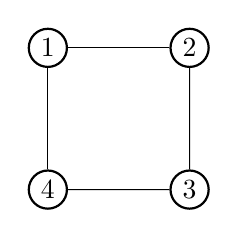
\begin{tikzpicture}
      \begin{scope}[scale=0.6]
        \tikzstyle{cnode} = [thick, draw=black, circle, inner sep = 2pt,  align=center]
        \node[cnode] (x1) at (0,0) {$1$};
        \node[cnode] (x2) at (3,0) {$2$};
        \node[cnode] (x3) at (3,-3) {$3$};
        \node[cnode] (x4) at (0,-3) {$4$};

        \draw[-] (x1) -- (x2);
        \draw[-] (x1) -- (x4);
        \draw[-] (x2) -- (x3);
        \draw[-] (x4) -- (x3);
      \end{scope}
    \end{tikzpicture}
  \end{subfigure}
  \begin{subfigure}{0.3\textwidth}
    \begin{tabular}{llc}
      \toprule
      $x_1$ & $x_2$ & $\phi(x_1, x_2)$ \\ %
      \midrule
      0  &  0  &  10 \\
      0  &  1  &  1 \\
      1  &  0  &  1 \\
      1  &  1  &  10\\
      \bottomrule
    \end{tabular}
  \end{subfigure}
  % \begin{subfigure}{0.05\textwidth}
  %   \centering
  %   \begin{tikzpicture}
  %     \node[] at (0,0) {$\cdots$};
  %   \end{tikzpicture}
  % \end{subfigure}
  \begin{subfigure}{0.3\textwidth}
    \begin{tabular}{llc}
      \toprule
      $x_2$ & $x_3$ & $\phi(x_2, x_3)$ \\
      \midrule
      0  &  0  &  5 \\
      0  &  1  &  3 \\
      1  &  0  &  3 \\
      1  &  1  &  5 \\
      \bottomrule
    \end{tabular}
  \end{subfigure}
  \begin{subfigure}{0.03\textwidth}
    \centering
    \begin{tikzpicture}
      \node[] at (0,0) {$\cdots$};
    \end{tikzpicture}
  \end{subfigure}
  \caption{A Markov random field with four binary nodes. Potential factors are represented by tables.}
  \label{chp2:fig:toy_mrf}
  \hspace{1cm}
\end{figure}

\begin{example}\label{chpt2:mrf-3node-example}
  As shown in Figure~\ref{chp2:fig:toy_mrf}, the MRF encodes the dependencies of four random variables $x_1$, $x_2$, $x_3$, and $x_4$, where node $i$ is associated with variable $x_i$ and each has a binary domain, i.e., $\Xx_i = \{0,1\}$ for $i =1, 2, 3, 4$. Four potential factors of the MRF together define the joint distribution
  \begin{equation*}
    p(\bm{x}) = \frac{1}{Z} \phi_{1,2}(x_1, x_2) \phi_{2,3}(x_2, x_3) \phi_{1,4}(x_1, x_4)\phi_{3,4}(x_3, x_4)
  \end{equation*}
  where $Z = \sum_{x_1, x_2, x_3, x_4}\phi_{1,2}(x_1, x_2) \phi_{2,3}(x_2, x_3) \phi_{1,4}(x_1, x_4)\phi_{3,4}(x_3, x_4)$ normalizes the potential factors such that $p(\bm{x})$ is a proper distribution. The exemplified potential factors in Figure~\ref{chp2:fig:toy_mrf} demonstrate that it is more compatible or likely when $x_1$, $x_2$ and $x_3$ are in the same state (either $0$ or $1$) than they are configured into different states.
\end{example}

From the above example to a formal statement, a MRF over random vector $\bm{x}$ can be represented by a undirected graph $\Gg(\Vv, \Ee)$, with each node $i \in \Vv$ is associated with a random variable $x_i$ and undirected edge set $\Ee \subset \Vv \times \Vv$. This MRF encodes a collection of distributions that factorize as
\begin{equation}\label{chp2:eq:mrf-definition}
  p(\bm{x};\bm{\theta}) = \frac{1}{Z(\bm{\theta})} \prod_{a \in \Ff} \phi_{a}(\bm{x}_{a};\bm{\theta}),
\end{equation}
where $\Ff$ is the set of indexes of potential factors, and each factor $\phi_{a}$ for $a\in \Ff$ is defined on subset of $\bm{x}$, i.e., $\phi_{a}: \Xx_{a} \rightarrow \RR^{+} \cup \{0\}$, where $\Xx_{a} = \prod_{i\in a}\Xx_i$ is the domain of potential factor $\phi_{a}$. The scope of factor $a$ is $\bm{x}_{a} = \left\{ x_i| i\in a \right\}$ where $i \in a$ stands for that the variable $x_i$ associated with node $i$ is an argument of potential factor $\phi_{a}$. In \eqref{chp2:eq:mrf-definition},
\begin{equation}
  Z(\bm{\theta}) = \sum_{\bm{x}} \prod_{a \in \Ff} \phi_{a}(\bm{x}_{a};\bm{\theta})
\end{equation}
is the \textit{partition function}. Obviously, the partition function normalizes the potential factors such that $p(\bm{x}; \bm{\theta})$ is a proper probability.

\begin{remark}[On set $\Ff$ of potential factors]
In our definition in \eqref{chp2:eq:mrf-definition}, the set of potential factors, i.e., $\Ff$, is not required to be the set of all \textit{maximal cliques} of the graph $\Gg$. A clique of the graph $\Gg$ is a subset of nodes in $\Gg$, within which any two nodes are connected by an edge of $\Gg$. A maximal clique is a clique such that it is not possible to include any other nodes from $\Gg$ into the clique without it ceasing to be a clique. Note there is literature that defines MRF over maximal cliques \cite[section~8.3.2]{Bishop:2006:PRM:1162264}. Actually, we can always reformulate \eqref{chp2:eq:mrf-definition} into factorization over maximal cliques by redefining a maximal clique as the product of potential factors (in $\Ff$) that are subsets of the maximal clique. Nevertheless, the definition in \eqref{chp2:eq:mrf-definition} without maximal clique requirement allows more flexibility of factorization and finer specification of potential factors. These properties may also benefit computations.
\end{remark}

\begin{remark}[Comparison of directed and undirected graphical models]
  We can compare directed and undirected graphical models with regard to the following aspects.
  \begin{itemize}
  \item \textit{Representation}: The structure and the parameterization in directed graphical models provide a natural representation for many types of real-world domains. For domains where interactions are naturally directional, directional graphical models can best manifest the abstraction and encode the dependencies. On the contrary, for domains where interactions are symmetrical without certain directionality, MRFs would be natural choices since forcing a directionality in these cases may cause an incomplete representation of dependencies. Furthermore, MRFs can be either cyclic or acyclic, which allows intuitive graphical representation with weaker constraint and gives the flexibility of graph structures.
  \item \textit{Local nonnegative functions}: The local functions are conditional probability functions in directed graphical models. In undirected graphical models, the local functions are potential factors that allow more flexible forms.
  \item \textit{Sampling}: Sampling is more straightforward within generative models (directed graphs) than that in MRFs.
  \item \textit{Normalization}: Since each local function is a conditional probability function in directed graphical models, the partition function for normalization is not needed. An MRF, in general, comes with a partition function, since potential factors are not necessarily normalized.
  \end{itemize}
\end{remark}

\begin{remark}[Graphical models with both directed and undirected edges]
  In the above discussions, we have presented both directed and undirected graphical models. In literature, a single graphical model may also encode both directed and undirected dependencies, i.e., there are both directed and undirected edges in its graph. Perhaps the most well-known models in this track are the \textit{conditional random fields} (CRFs). See \cite{charles2012crf} for more introduction.
\end{remark}


\subsection{An Alternative Representation}
\begin{figure}[!t]
  % \captionsetup[subfigure]{justification=centering}
  \begin{subfigure}{.33\textwidth}
    \centering
    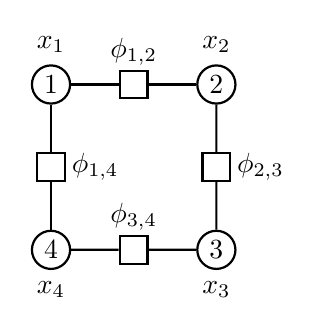
\begin{tikzpicture}
      \begin{scope}[scale=0.7]
        \tikzstyle{cnode} = [thick, draw=black, circle, inner sep = 2pt,  align=center]
        \tikzstyle{nnode} = [thick, rectangle, rounded corners = 0pt,draw,inner sep = 5pt]
        \node[cnode] (x1) at (0,0) {$1$};
        \node[above=0.2mm of x1] {$x_1$};
        \node[cnode] (x2) at (3,0) {$2$};
        \node[above=0.2mm of x2] {$x_2$};
        \node[cnode] (x3) at (3,-3) {$3$};
        \node[below=0.2mm of x3] {$x_3$};
        \node[cnode] (x4) at (0,-3) {$4$};
        \node[below=0.2mm of x4] {$x_4$};

        
        \node[nnode] (f12) at (1.5, 0) {};
        \node[] at ($(f12) + (0,0.6)$) {$\phi_{1,2}$};
        \node[nnode] (f34) at (1.5, -3) {};
        \node[] at ($(f34) + (0,0.6)$) {$\phi_{3,4}$};
        
        \node[nnode] (f14) at (0, -1.5) {};
        \node[] at ($(f14) + (0.8,0)$) {$\phi_{1,4}$};
        \node[nnode] (f23) at (3, -1.5) {};
        \node[] at ($(f23) + (0.80,0)$) {$\phi_{2,3}$};
        \path[-, draw, thick]
        (x1) edge node {} (f12)
        (f12) edge node {} (x2)
        (x2) edge node {} (f23)
        (f23) edge node {} (x3)
        (x3) edge node {} (f34)
        (f34) edge node {} (x4)
        (x4) edge node {} (f14)
        (f14) edge node {} (x1)
        ;
      \end{scope}
    \end{tikzpicture}
    \caption{A factor graph representation.}
    \label{chpt2:fig:factor-graph-3node-example}
  \end{subfigure}
  \begin{subfigure}{.33\textwidth}
    \centering
    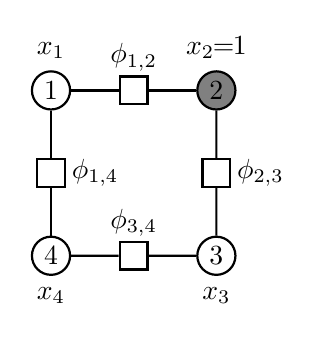
\begin{tikzpicture}
      \begin{scope}[scale=0.7]
        \tikzstyle{cnode} = [thick, draw=black, circle, inner sep = 2pt,  align=center]
        \tikzstyle{cfnode} = [thick, draw=black, fill=gray,circle, inner sep = 2pt,  align=center]
        \tikzstyle{nnode} = [thick, rectangle, rounded corners = 0pt,draw,inner sep = 5pt]

        \node[cnode] (x1) at (0,0) {$1$};
        \node[above=0.2mm of x1] {$x_1$};
        \node[cfnode] (x2) at (3,0) {$2$};
        \node[above =0.2mm of x2] {$x_2\!\!=\!\!1$};
        \node[cnode] (x3) at (3,-3) {$3$};
        \node[below=0.2mm of x3] {$x_3$};
        \node[cnode] (x4) at (0,-3) {$4$};
        \node[below=0.2mm of x4] {$x_4$};

        
        \node[nnode] (f12) at (1.5, 0) {};
        \node[] at ($(f12) + (0,0.6)$) {$\phi_{1,2}$};
        \node[nnode] (f34) at (1.5, -3) {};
        \node[] at ($(f34) + (0,0.6)$) {$\phi_{3,4}$};
        
        \node[nnode] (f14) at (0, -1.5) {};
        \node[] at ($(f14) + (0.8,0)$) {$\phi_{1,4}$};
        \node[nnode] (f23) at (3, -1.5) {};
        \node[] at ($(f23) + (0.80,0)$) {$\phi_{2,3}$};
        \path[-, draw, thick]
        (x1) edge node {} (f12)
        (f12) edge node {} (x2)
        (x2) edge node {} (f23)
        (f23) edge node {} (x3)
        (x3) edge node {} (f34)
        (f34) edge node {} (x4)
        (x4) edge node {} (f14)
        (f14) edge node {} (x1)
        ;
      \end{scope}
    \end{tikzpicture}
    \caption{Conditioning on $x_2=1$ in factor graph.}
    \label{chpt2:fig:factor-graph-3node-example-condition}
  \end{subfigure}
  \begin{subfigure}{.3\textwidth}
    \centering
    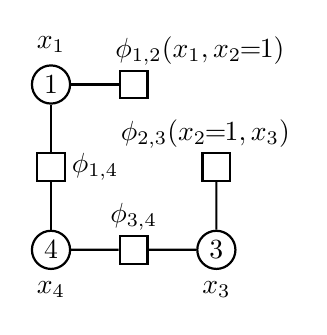
\begin{tikzpicture}
      \begin{scope}[scale=0.7]
        \tikzstyle{cnode} = [thick, draw=black, circle, inner sep = 2pt,  align=center]
        \tikzstyle{cfnode} = [thick, draw=black, fill=gray,circle, inner sep = 2pt,  align=center]
        \tikzstyle{nnode} = [thick, rectangle, rounded corners = 0pt,draw,inner sep = 5pt]


        \node[cnode] (x1) at (0,0) {$1$};
        \node[above=0.2mm of x1] {$x_1$};
        \node[cnode] (x3) at (3,-3) {$3$};
        \node[below=0.2mm of x3] {$x_3$};
        \node[cnode] (x4) at (0,-3) {$4$};
        \node[below=0.2mm of x4] {$x_4$};

        
        \node[nnode] (f12) at (1.5, 0) {};
        \node[] at ($(f12) + (1.2,0.6)$) {$\phi_{1,2}(x_1, x_2\!\!=\!\! 1)$};
        
        \node[nnode] (f34) at (1.5, -3) {};
        \node[] at ($(f34) + (0,0.6)$) {$\phi_{3,4}$};
        
        \node[nnode] (f14) at (0, -1.5) {};
        \node[] at ($(f14) + (0.8,0)$) {$\phi_{1,4}$};
        \node[nnode] (f23) at (3, -1.5) {};
        \node[] at ($(f23) + (-0.2,0.6)$) {$\phi_{2,3}(x_2\!\!=\!\! 1, x_3)$};

        \path[-, draw, thick]
        (x1) edge node {} (f12)

        (f23) edge node {} (x3)
        (x3) edge node {} (f34)
        (f34) edge node {} (x4)
        (x4) edge node {} (f14)
        (f14) edge node {} (x1)
        ;
      \end{scope}
    \end{tikzpicture}
    \caption{The reduced graph of Figure~\ref{chpt2:fig:factor-graph-3node-example-condition}}
    \label{chpt2:fig:factor-graph-3node-example-reduced}
  \end{subfigure}
  
  \caption{A Markov random field is represented by a factor graph, i.e., \ref{chpt2:fig:factor-graph-3node-example}. Conditioning of the MRF in \ref{chpt2:fig:factor-graph-3node-example-condition}. The reduced MRF in \ref{chpt2:fig:factor-graph-3node-example-reduced}.}
  \label{chp2:tab:toy-factor-graph}
  \hspace{1cm}
\end{figure}

The previous graphical representations do not explicitly include the conditional probability functions or potential factors in their graphs. An alternative representation to a graphical model (undirected or directed) is \textit{factor graph} \cite{kschischang2001factor_graph},
which is a bipartite graph topology. In a factor graph, a potential factor or a conditional probability funciton is explicitly represented as a factor node, as the counterpart of the variable node associated with a random variable. We focus on the correspondence between a MRF and its factor graph here.
\begin{definition}\label{chpt2:def:factor-graph}
  A factor graph $\Gg_F$, is a bipartite graph that represents the factorization of \eqref{chp2:eq:mrf-definition}. A factor graph has two types of nodes: i) a variable node for each variable $x_i$; ii) a factor node for each potential function $\phi_{a}$. An edge is placed between a variable node $i$ and factor node $a$ if and only if $x_i$ is argument of $\phi_{a}$. We denote a factor graph by $\Gg_F(\Vv \cup \Ff, \Ee_F)$ with $\Vv$ as the set of variable nodes, $\Ff$ as the set of factor nodes, and $\Ee_F$ the set of undirected edges.
\end{definition}
\begin{example}
  Let us represent the Example~\ref{chpt2:fig:factor-graph-3node-example} by a factor graph, which is shown in Figure~\ref{chpt2:fig:factor-graph-3node-example}. Different from the representation by $\Gg(\Vv, \Ee)$ in Figure~\ref{chp2:fig:toy_mrf}, factor nodes are explicitly represented by square nodes.
\end{example}


\subsection{Conditioning on Observations in MRFs}
It is not rare that a graphical model may contain observed variable. The node set of a MRF can be separated into a subset $\Vv_O$ of nodes that are associated with observed variable $\bm{x}_O$, and a subset $\Vv_U$ of nodes associated with unobserved variable $\bm{x}_U$. When an evidence is observed, its likelihood can be computed as
\begin{equation}
  p(\bm{x}_O;\bm{\theta}) = \sum_{\bm{x}_U} p(\bm{x};\bm{\theta}) =\sum_{\bm{x}_U}\frac{\tilde{p}(\bm{x}; \bm{\theta})}{Z(\bm{\theta})} = \frac{Z(\bm{x}_O,\bm{\theta})}{Z(\bm{\theta})},
\end{equation}
where 
\begin{align}
  \tilde{p}(\bm{x}; \bm{\theta}) &= \prod_{a \in \Ff} \phi_{a}(\bm{x}_{a};\bm{\theta}), \nonumber \\
  Z(\bm{x}_O, \bm{\theta}) &= \sum_{\bm{x}_U} \tilde{p}(\bm{x}; \bm{\theta}), \nonumber \\
  Z(\bm{\theta}) &= \sum_{\bm{x}_O}\sum_{\bm{x}_U} \tilde{p}(\bm{x}; \bm{\theta}).
\end{align}
This means that the likelihood of an (partial) evidence can be computed by partition function and sub-partition functions. As shall be seen in Part~\ref{part:learning}, this likelihood function, or its appropriations would be used for model learning.

 When an evidence $\bm{e}_O$ (an sample instance of $\bm{x}_O$) is observed, the conditional probability can be written as
\begin{equation}\label{chpt2:eq:mrf-condtioning}
  p(\bm{x}_U|\bm{x}_O=\bm{e}_O;\bm{\theta}) = \frac{\tilde{p}(\bm{x}_U, \bm{x}_O = \bm{e}_O; \bm{\theta})}{\sum_{\bm{x}_U}\tilde{p}(\bm{x}_U, \bm{x}_O = \bm{e}_O; \bm{\theta})} \propto \tilde{p}(\bm{x}_U, \bm{x}_O = \bm{e}_O; \bm{\theta}),
\end{equation}
where $\propto$ stands for proportional to. \eqref{chpt2:eq:mrf-condtioning} shows an interesting phenomenon for MRF including evidence. It can be understood as clamping nodes in $\Vv_O$ of the MRF to configuration $\bm{e}_O$, i.e., the domain of $\bm{x}_O$ becomes a set containing only one instance $\bm{e}_O$. For instance, an example of conditioning on a variable node for Example~\ref{chpt2:mrf-3node-example} is shown in Figure~\ref{chpt2:fig:factor-graph-3node-example-condition}, where node $2$ is clamped to evidence $x_2=1$.



In addition to the above intuitions, conditioning can also be understood as a process of reducing the graph of an MRF. When an MRF is conditioned on $\bm{x}_O$, the variables nodes of set $\Vv_O$ are removed from $\Gg$, along with their edges. The potential factors with regard to $\Vv_U$ are modified accordingly \cite[Chapter~4.2.3]{koller2009pgm}. For instance,
the graph including evidence node $2$ in Figure~\ref{chpt2:fig:factor-graph-3node-example-condition} can be further reduced into a Figure~\ref{chpt2:fig:factor-graph-3node-example-reduced}. Then any inference applicable to an MRF applies to the MRF with nodes clamped as well. An MRF with several nodes clamped to some evidence can be seen either as a manipulation of its domain or the graph itself.


It can be seen that the MRF framework is capable of handling evidence and conditioning as well. We would come back to this topic in Part~\ref{part:learning}.

\section{Divergence}\label{chpt2:sec:devergence}
Before we get into further discussions about inference and learning, we first introduce the concept of \textit{divergence} measures since principles of both learning and inference are closed related to divergence measures.
A divergence measure plays a fundamental role when we try to use a probability distribution (over discrete or continue variable)  $q$ to approximate another probability distribution $p$. A divergence measure is used to formally quantity how much information is lost when $p$ is represented by $q$. Denote $\PP$ as the space of measures $p$ and $q$, i.e., $p, q \in \PP$.
\begin{definition}
  Given the space $\PP$ of probability distribution for a random variable $\bm{x}$, a divergence on this space is defined as a function $D(p\|q): \PP \times \PP \rightarrow \RR^{+}\cup \{0\}$ such that $D(p\|q) \geq 0$ for all $p, q \in \PP$ and $D(p\|q)=0$ if and only if $p=q$.
\end{definition}

Here we introduce the classic \textit{Kullback-Leibler divergence} \cite{kullback1959, kullback1951}, KL divergence for short, which is one of the most widely used divergence measures in machine learning, statistics and information theory.
\begin{definition}
  The Kullback-Leibler (KL) divergence on $\PP$ is defined as a function $KL(\cdot \| \cdot): \PP \times \PP \rightarrow \RR^{+} \cup {0}$ with the following form
  \begin{equation}\label{chpt2:def:kl-divergence}
    \mathrm{KL}(p\|q) = \sum_{\bm{x}}p(\bm{x}) \log{\frac{p(\bm{x})}{q(\bm{x})}},
  \end{equation}
  where $\log$ is the natural loggarithm. Note the sum in \eqref{chpt2:def:kl-divergence} should be replaced by intergral when $p$ and $q$ are probability density functions.
\end{definition}


KL divergence is not symmetric. In another word, there is no equivalence between $\mathrm{KL}(p\|q)$ and $\mathrm{KL}(q\|p)$ in general. A symmetric divergence that generalizes the KL divergence would be introduced in Section~\ref{chpt3:sec:alpha-divergence}. Furthermore, an extra metric that is used to compare distributions, i.e., optimal transport, would be introduced in Section~\ref{chpt8:sec:ot}.



\section{Inference Tasks}


Given a probability distribution $p(\bm{x})$ as the underlying distribution of a graphical model, inference in general can be divided into four kinds of tasks, as explained in Chapter~\ref{chpt1:sec:scope-outline}. Our work in this thesis is closely involved with the problems
\begin{itemize}
\item computing the likelihood of observed data or unobserved random variable;
\item computing the marginals distribution over a particular subset of nodes, i.e., $p(\bm{x}_A)$ for $A \subset \Vv$. Note that a single-node marginal distribution $p(x_i)$ also belongs to this case;
\item computing the conditional distribution a subset of nodes given the configuration of another subset of nodes, i.e., $p(\bm{x}_A| \bm{x}_B)$ for $A, B \in \Vv$ and $A \cap B = \emptyset$;
\end{itemize}
in MRFs. The above tasks are also closely related with the inference of the partition function, i.e.,
\begin{itemize}
\item computation of $Z(\bm{\theta}) = \sum_{\bm{x}} \prod_{a \in \Ff} \phi_{a}(\bm{x}_{a};\bm{\theta})$, or sub-partition functions.
\end{itemize}

In the following section, we introduce the methods for the above tasks at a high-level.

\section{Exact Inference}
\label{chpt2:sec:inference-mp}
In this section, we briefly treat the exact inference of graphical models. Please see \cite{Bishop:2006:PRM:1162264, koller2009pgm, yedida2005constucting, yedidia2003understanding} for detailed discussions. In order to compute a marginal probability, we need to sum or integrate the joint probability distribution over some variables. This operation can be performed as a sequence of operations by a pre-defined ordering of the variables. Since the underline distribution of a graphic model (directed or undirected) is a product of factors, the sequence or order can be chosen in a way that facilitates the sum or integral operations. Thus the computation of the marginal probability is up to choose a specific ordering of remaining variables to eliminate (sum or integrate out) repeatedly. This brings the very fundamental exact inference method, \textit{variable elimination}.

When we want to ask multiple queries (marginal probabilities) on a graphical model, we repetitively call the variable elimination method for each query until all queries are answered. The \textit{sum-product} algorithm is more efficient for this case. It is a \textit{message passing} algorithm that operates on graphical models. More importantly, the intermediate results, the messages, are shared in all computations. Thus one call of this message passing algorithm returns answers to multiple queries. The sum-product algorithm, also known as \textit{belief propagation}, has an iterative message update rule. A message update step from a factor $a$ to its neighboring variable node $i$ is 
\begin{equation}\label{chpt2:eq:loopy-bp}
  m_{a\rightarrow i}(x_i) \propto \sum_{\bm{x}_{a} \backslash x_i}
  \phi_{a}(\bm{x}_{a}) \prod_{j \in a \backslash i} \prod_{a^{\prime} \in \mathrm{ne}_j
    \backslash a} m_{a^{\prime}\rightarrow j}(x_j),
\end{equation}
where $a^\prime, a \in \Ff$ and $\mathrm{ne}_i = \left\{ a | i \in a, a \in \Ff \right\}$ denotes the neighboring factors of the variable node $i$. The left-hand-side of $\propto$ is the updated message and the right-hand-side of $\propto$ is a function of factors and old messages in \eqref{chpt2:eq:loopy-bp}. The marginal for $x_i$ is simply $p(x_i)\propto\prod_{a\in\mathrm{ne}_i}m_{a\rightarrow i}(x_i)$ after all messages have been updated accordingly. For a tree-structured graph, the message passing rule in \eqref{chpt2:eq:loopy-bp} with pre-defined ordering of sequential updates gives exact marginals.

However, when a graphical model is not tree-structured, the above methods can not give exact inference. If exact inference is still desired here, one may consider converting the graph of the graphical model into a clique tree, an acyclic graph whose nodes are maximal cliques, and apply the \textit{junction tree} algorithm.

It is known that the computational complexity of the junction tree method grows exponentially in the size of the maximal clique. Therefore, for certain classes of graphs, exact inference is feasible by using the methods mentioned above. On the other hand, there are many graphical models where exact inference is too expensive in computation or simply prohibitive. We need to turn to approximate inference to cope with such models.


\section{Variational Inference}
\label{chpt2:sec:variational-inference}

In solving inference tasks with approximation, one important technique is based on a variational approach. With $p(\bm{x};\bm{\theta})$ as the underlining probability distribution of a graphical model, directly inference with $p(\bm{x}; \bm{\theta})$ is often unfeasible due to the system represented by the graphical model is too large or complex. It can also be the case that even we know the form of $p(\bm{x}; \bm{\theta})$, the computation in inference tasks can be prohibitive. In variational approaches, a 'trial' probability distribution $b(\bm{x})$ is introduced to approximate $p(\bm{x};\bm{\theta})$. The trial distribution should be intuitively simpler than $p(\bm{x}; \bm{\theta})$. \textit{Variational free energy} \cite{opper2001advanced} is a quantity used to find such a approximation. The variational free energy is defined by
\begin{align}\label{chpt2:eq:variational-free-energy}
  F_V(b) & = \mathrm{KL}(b( \bm{x}) || p(\bm{x}; \bm{\theta})) - \log{Z(\bm{\theta})} \nonumber \\
         &= \sum_{\bm{x}}b(\bm{x}) \log{\frac{b(\bm{x})}{{p}(\bm{x}; \bm{\theta})}} - \log{Z(\bm{\theta})} \nonumber \\
         & = \sum_{\bm{x}}b(\bm{x}) \log{\frac{b(\bm{x})}{\tilde{p}(\bm{x}; \bm{\theta})}},
\end{align}
where $\tilde{p}(\bm{x}; \bm{\theta}) =  \prod_{a \in \Ff} \psi_{a}(\bm{x}_{a}; \bm{\theta}_{a})$. Since $\mathrm{KL}(b(\bm{x})\|p(\bm{x};\bm{\theta}))$ is always non-negative and is zero if and only if $b(\bm{x}) = p(\bm{x};\bm{\theta})$, we have $F_V(b) \geq - \log{Z(\bm{\theta})}$, with equality when $b(\bm{x}) = p(\bm{x};\bm{\theta})$.

\begin{remark}
  Note from \ref{chpt2:eq:variational-free-energy}, the minimization w.r.t. $b$ of variational free energy is equivalent to the divergence minimization, i.e., $\mathrm{KL}(b( \bm{x}) || p(\bm{x}; \bm{\theta}))$, since $\log{Z(\bm{\theta})}$ does not depend on $b$. By observing $F_V(b) = \sum_{\bm{x}}b(\bm{x}) \log{\frac{b(\bm{x})}{\tilde{p}(\bm{x}; \bm{\theta})}}$, the free energy minimization guides the choice of $b$ such that $b$ is close to an unnormalized measure $\tilde{p}(\bm{x}; \bm{\theta})$ in its space.

  Another benefit of \ref{chpt2:eq:variational-free-energy} is that we are able to approximate $p(\bm{x}; \bm{\theta})$ without inference of the true marginal distributions $\{p(\bm{x}_{a};\bm{\theta}), a \in \Ff\}$. Since $\log\tilde{p}(\bm{x}; \bm{\theta})$ can be formulated as sum of log-potential-factors that are all local functions, the computation of $F_V(v)$ can be done by inference of marginals $\left\{ b_{a}(\bm{x}_{a}), a \in \Ff \right\}$ of the approximate distribution, which are tractable.
\end{remark}

\begin{remark}
  Discussion: Since we are essentially approximating distribution $p$ by a distribution $b$, can we minimize $\mathrm{KL}(p(\bm{x}, \bm{\theta})\|b(\bm{x}))$ instead?

  It might be feasible by instinct. But a further check would reveal its infeasibility. The $\mathrm{KL}(p(\bm{x}; \bm{\theta})\|b(\bm{x}))$ would inevitable requires the marginals of $p$ and therefore requires the exact inference in $p$, which are what we are trying to avoid. But it does not mean this divergence is useless. As shall be seen in \autoref{chpt2:sec:learning-principles}, this type of divergence measure is what we need in model learning.
\end{remark}



\subsection{Variational Free Energy and Mean Field}

Mean field method, similar to the sum-product algorithm in Section~\ref{chpt2:sec:inference-mp}, is an iterative message passing approach. 
The message update rule of mean field algorithm is described as follow.
\begin{equation}\label{chpt2:eq:mf-update}
  \log{b_i(x_i)} \propto \sum_{a \in \mathrm{ne}_i} \sum_{\bm{x}_{a} \backslash x_i} \log{\phi_{a}}(\bm{x}_{a};\bm{\theta}_{a}) \prod_{j\in {a}\backslash i} b_j(x_j).
\end{equation}
The algorithm does iterative update of the belief on each node of the graphical model. An update step for node $i$ use its neightbors' old  beliefs  $\left\{ b_j(x_j), j\in {a}\backslash i, a \in \mathrm{ne}_i \right\}$ and factors to assign new belief $b_i(x_i)$. After the iterative algorithm converges, the approximation to marginal $p(x_i)$ is $b_i(x_i)$.


The intuition of mean field algorithm can be given by the variational free energy defined in Section~\ref{chpt2:sec:variational-inference}. In fact, mean field approach uses the fully-factorized distribution,
\begin{equation}\label{eq:mf-factorization}
  b_{MF}(\bm{x}) = \prod_{i=1}^{N}b_i(x_i),
\end{equation}
to approximate the joint distraction $p(\bm{x};\bm{\theta})$. The update rule \eqref{chpt2:eq:mf-update} can be obtained by minimizing the 'difference' between the fully-factorized distribution and $p(\bm{x};\bm{\theta})$, i.e., the variational free energy \eqref{chpt2:eq:variational-free-energy}. Specifically,
substituting \eqref{eq:mf-factorization} into the variational free energy \eqref{chpt2:eq:variational-free-energy} gives
\begin{align}
  F_{MF}(b) =  - \sum_{a \in \Ff}\sum_{\bm{x}_{a}} \log{\phi_{a}(\bm{x}_{a};\bm{\theta})}
  \prod_{i\in a}b_i(x_i) + \sum_{i \in \Vv} \sum_{x_i} b_i(x_i) \log{b_i(x_i)}.
\end{align}
Minimizing $F_{MF}(b)$ over $\left\{ b_i \right\}$ would give us the mean field update rule \eqref{chpt2:eq:mf-update}.

\subsection{Bethe Free Energy and (Loopy) Belief Propagation}

We described the sum-product algorithm (belief propagation) for exact inference in tree-structured graphs in Section~\ref{chpt2:sec:inference-mp}. For graphical models with the presence of cycles or loops, we can still apply the sum-product algorithm as if there was no loop. This is known as the loopy belief propagation (loopy BP). Of course, the inference results are no longer exact anymore. But loopy BP still works well in many practical cases.

Now we give the intuition of loopy BP from the perspective of free energy minimization, which comes with the name of Bethe approximation in literature.
Different from the mean field approximation, Bethe approximation also includes the non-single-node beliefs $\{b_{a}(\bm{x}_{a})\}$ apart from the single-node beliefs $\{b_i(x_i)\}$\cite{yedidia2003understanding}. In this case, the Bethe free energy is given by
\begin{align}\label{chpt2:bethe-free-energy}
  F_{Bethe}(b) = \sum_{a} \sum_{\bm{x}_{a}}
  b_{a}(\bm{x}_{a})\log{\frac{b_{a}(\bm{x}_{a})}{\phi_{a}(\bm{x}_{a})}
  } -  \sum_{i=1}^{N} (|\mathrm{ne}_i| - 1) \sum_{x_i} b_i(x_i) \log{b_i(x_i)},
\end{align}
where $|\cdot|$ stands for carnality.
Due to the  non-single-node beliefs, there are consistency constrains $\sum_{\bm{x}_{a}} b_{a}(\bm{x}_{a}) = \sum_{ x_i} b_i({x}_i) =1$, $\forall~ i \in a$ to obey. Then, solving the Bethe free energy minimization problem
\begin{align}
  \min_{\{b_{a}(\bm{x}_{a})\}, \{b_i(x_i)\}}& F_{Bethe}(b) \nonumber \\
  \mathrm{s.t.}~~ & \sum_{\bm{x}_{a} \backslash x_i} b_{a}(\bm{x}_{a})  =
                    b_i(x_i), \nonumber \\
                                                      & \sum_{\bm{x}_{a}} b_{a}(\bm{x}_{a}) = \sum_{ x_i} b_i({x}_i) =1,
                                                        \nonumber \\
                                                      &  0 \leq b_i(x_i) \leq 1,  \nonumber \\
                                                      & i \in \Vv , a \in \Ff,
\end{align}
where $\Vv$ and $\Ff$ are the set of variable nodes and the set of
factor nodes in factor graph as defined in
Definition~\ref{chpt2:def:factor-graph}, gives the (loopy) BP message passing rule that has the same formula as in \eqref{chpt2:eq:loopy-bp}.

These variational approaches would be further discussed and compared in Chapter~\ref{chapter3} and \ref{chapter4} of Part~\ref{part:inference}.

\section{Learning Principles}
\label{chpt2:sec:learning-principles}
We have touched the learning topic in Chapter~\ref{chapter1}, which is to find the 'best' probability distribution $p(\bm{x}; \bm{\theta})$ in its space $\PP$. To make the discussion more concrete, we assume the domain is governed by a underlying distribution $p^{\ast}$ that is induced by a (directed or undirected) graphical model, $\Mm^{\ast} = \left\{ \Kk^{\ast}, \bm{\theta}^{\ast} \right\}$ with $\Mm^{\ast}$ representing its structure and $\bm{\theta}^{\ast}$ representing its parameter. Here we discuss about \textit{model learning} (parameter learning only). For notation simplicity, we use $p^{\ast}(\bm{x})$ to denote this distribution. We are given a dataset $\Dd = \{\bm{x}^{1}, \bm{x}^{2}, \cdots, \bm{x}^{M}\}$. Following the standard assumption, these sample instances are \textit{independent and identically distributed (i.i.d.)} according to $p^{\ast}(\bm{x})$. The task is then to use the information from the dataset to learn a distribution $p(\bm{x};\bm{\theta})$ within its space $\PP$, since the governing distribution $p^{\ast}(\bm{x})$ is not known.

The problem of learning a distribution in $\PP$ to approximate $p^{\ast}$ can be formulated as density estimation. With the concept of KL divergence in Section~\ref{chpt2:sec:devergence}, learning of $p(\bm{x};\bm{\theta})$ can be formulated as minimizing the KL divergence
\begin{align}\label{chpt2:sec:mle-as-min-kl}
  &\mathrm{KL}(p^{\ast}(\bm{x})\|p(\bm{x}; \bm{\theta})) \nonumber \\
  =& \EE_{p^{\ast}(\bm{x})}\left[ \log{\frac{p^{\ast}(\bm{x})}{p(\bm{x}; \bm{\theta})}} \right] \nonumber \\
  =& - H(p^{\ast}) - \EE_{p^{\ast}(\bm{x})}\left[ \log{{p(\bm{x}; \bm{\theta})}} \right],
\end{align}
where $H(p^{\ast})$ is the entropy of $p^{\ast}$.
Due to the property of divergence, the KL divergence in \eqref{chpt2:sec:mle-as-min-kl} is zero if and only if $p(\bm{x};\bm{\theta})=p^{\ast}(\bm{x})$. The last line of \eqref{chpt2:sec:mle-as-min-kl} shows that the negative entropy term does not depend on $p(\bm{x}; \bm{\theta})$. Thus we can just focus on the expectation term $\EE_{\bm{x} \sim p^{\ast}}\left[ \log{{p(\bm{x}; \bm{\theta})}} \right]$, which is \textit{expected log-likelihood}. Therefore, we can just use the expected log-likelihood to do model learning.

Note although we can use the expected log-likelihood for the model learning task and for even model comparison (comparing a trained model with another one), we lose the information of how close a trained model is to $p^{\ast}$. This is due to the omitting of $H(p^{\ast})$, which is not available.

Since it is not possible to know $p^{\ast}$ (otherwise we do not need to learn it), the expected log-likelihood is approximated by sample instances of $p^{\ast}$,
\begin{equation}
  \Ll(\Dd; \bm{\theta}) = \frac{1}{\abs{\Dd}}\sum_{\bm{x}\in \Dd}\log{p(\bm{x};\bm{\theta})},
\end{equation}
and
\begin{equation}
  \EE_{p^{\ast}(\bm{x})}\left[ \log{{p(\bm{x}; \bm{\theta})}} \right] \approx \Ll(\Dd; \bm{\theta}).
\end{equation}


The log-likelihood $\Ll(\Dd; \bm{\theta})$ is one of the most widely used loss for model learning. However, $\Ll(\Dd; \bm{\theta})$ is not always a feasible loss to compute (see Chapter~\ref{chpt5:undirecteLearning} for more analyses) since
\begin{itemize}
\item it is often that exact computation of $p(\bm{x};\bm{\theta})$ is not possible; or
\item there are some elements of $\bm{x}$ which are not observable (hidden or latent variables).
\end{itemize}
For the first case, the typical treatment is to approximate the exact log-likelihood. This is done via approximation by employing inference methods or   making simplified assumptions on dependency structure of the graphical model of $p(\bm{x})$. Then, optimization is carried out with regard to the approximated log-likelihood. These methods include surrogate likelihood \cite{wainwright06estimating, lu2019blockBP}, pseudo-likelihood\cite{qu2019gmnn, lazarogredilla2019learning}, piecewise likelihood \cite{sutton2012piecewise, lin_2016_CVPR}, saddle-point approximation \cite{srikumar-etal-2012-amortizing, NIPS2019_9687}.

Apart from the above case where all variables are observable, the partial observed models, the latent variable case, are equally import in inference and learning with uncertainty. This class of models includes (but is not limited to) classic Gaussian mixture models (GMMs) and hidden Markov models (HMMs). There are latent variables because:
\begin{itemize}
\item Use of abstract variables to model the generative process (usually a directed graph) of observation data, such as HMMs.
\item A practical true attribute of an object may be difficult or impossible to measure exactly. For instance, the disease infection can only be diagnosed via the relevant symptoms, see e.g., Example~\ref{example-corona}. In the position tracking of a car with noisy sensors, the true position of the car might only be inferred via noisy data of sensors.
\item No measurement on an attribute of an object of interest is made. For instance, the velocity sensor in the car tracking example might not be stable and might fail from time to time.
\end{itemize}
In general, latent variables are commonly used to deal with partial observation problems, data clustering, data manipulation, etc. Let us denote the observable variable and latent variable by $\bm{x}_O$ and $\bm{x}_U$, respectively. We can see that the log-likelihood $p(\bm{x}_O, \bm{x}_U; \bm{\theta})$ is not available anymore as it is in the fully-observed case. To deal with the latent variables, we can try to optimize the partial log-likelihood
\begin{align}
  l(\bm{x}_O; \bm{\theta}) =& \log{p(\bm{x}_O; \bm{\theta})} \nonumber \\  
  = & \EE_{q(\bm{x}_U|\bm{x}_O)}\left[ \log{\frac{q(\bm{x}_U|\bm{x}_O)}{p(\bm{x}_U|\bm{x}_O;\bm{\theta})} \cdot \frac{p(\bm{x}_U,\bm{x}_O;\bm{\theta})}{q(\bm{x}_U|\bm{x}_O)}} \right] \nonumber \\
  = & \mathrm{KL}(q(\bm{x}_U|\bm{x}_O)\|p(\bm{x}_U|\bm{x}_O;\bm{\theta})) + F(q, \bm{\theta})
\end{align}
with
\begin{equation}\label{chpt2:eq:llk-lower-bound}
  F(q, \bm{\theta}) = \EE_{q(\bm{x}_U|\bm{x}_O)}\left[ \log{p(\bm{x}_U,\bm{x}_O;\bm{\theta})} \right] + H(q(\bm{x}_U|\bm{x}_O))
\end{equation}
where $H(q(\bm{x}_U|\bm{x}_O))$ is the entropy of $q(\bm{x}_U|\bm{x}_O)$, and $q$ can be any distribution over $\bm{x}_U$. Due to the non-negative property of KL divergence, we have
\begin{equation}
  l(\bm{x}_O; \bm{\theta}) \geq F(q, \bm{\theta}),
\end{equation}
with equality when $q(\bm{x}_U|\bm{x}_O) = p(\bm{x}_U|\bm{x}_O; \bm{\theta})$. $F(q, \bm{\theta})$ is also called \textit{variational lower bound}.

One of the most widely used methods in learning with latent variable is \textit{expectation maximization (EM)} \cite{DEMP1977em}. In the EM method, the posterior of $\bm{x}_U$ is computed exactly from $p$, $q(\bm{x}_U|\bm{x}_O) = \argmax_{q}{F(q, \bm{\theta})} = p(\bm{x}_U|\bm{x}_O; \bm{\theta})$, which is the optimal solution to $q$. Then the parameter $\bm{\theta}$ of $p$ is optimized. The two steps are optimized iteratively. The detailed treatment can be found in Part~\ref{part:learning}

In cases where the posterior of $\bm{x}_U$ is not feasible to compute, the variational EM\cite[section~6.2.2]{wainwright2008graphical} or Monte Carlo EM (need sampling technique) \cite{neath2012convergence} can be applied. There are also neural network based methods with Monte Carlo estimator to cope with the latent variable problems, see e.g., \cite{DBLP:journals/corr/KingmaW13, kuleshov2017NVIL, lazarogredilla2019learning, goodfellow2014gan}.


In the above discussion, we have assumed that the model's distribution $q$ is explicitly defined, i.e., the distribution (along with its density function or mass function) is available. 

In an alternative track, deep generative models grow popularity in literature and can be applied to different areas such as high-dimensional data representation, reinforcement learning, and semi-supervised learning, because of its efficient sampling of multi-mode distributions \cite{2017arXiv170100160G}. A generator in a deep generative model induces a distribution that can either be an explicit or implicit distribution. The former problem dates back to \cite{deco1995high-order} and receives more attention in recent years with latest work such as variational autoencoder \cite{DBLP:journals/corr/KingmaW13}, normalizing flows \cite{2016arXiv160508803D, 2018arXiv180703039K} and neural ordinary difference equations \cite{ricky2018ODE}. The training of explicit models is based on the maximum likelihood principle or variational likelihood bound. Chapter~\ref{chpt6:em-flow} and \ref{chpt7:genhmm} would give detailed treatment with modeling and learning with normalizing flows. Chapter~\ref{chapter9} will further discuss the implicit deep generative models and their learning.

The latter case brings an implicit distribution, where the maximum likelihood principle is not applicable anymore. In this case, a state-of-art method is the generative adversarial model that employs a discriminator to play the role of divergence measure \cite{goodfellow2014gan, 2017arXiv170104862A, NIPS2016_6125}, which is essentially explained by a process of the minimization of the Jensen-Shannon divergence. Additionally, other sample-test based distances are employed as alternative methods for implicit model learning. Among this family, optimal transport is receiving more attention in recent years \cite{santambrogio2015optimal, 2013arXiv1306.0895C} in this track, which has also been applied for training of Boltzmann machine \cite{NIPS2016_6248} auto-encoders\cite{2017arXiv171101558T} and generative adversarial networks \cite{2017arXiv170107875A}. We would discuss this further in Chapter~\ref{chapter9}.



%%% Local Variables:
%%% mode: latex
%%% TeX-master: "../../main"
%%% End:


\part{Inference}
\label{part:inference}
% chapter 3
\chapter{An Alternative View of Belief Propagation}
\label{chapter3}
% set the path to figures in this section
\graphicspath{{source/chapter3/}}

Belief propagation (BP) is a meta message-passing algorithm for inference problems in probabilistic graphical models. BP answers queries by locally exchanging beliefs (statistical information) between nodes in a graphical model \cite{kschischang2001factor_graph, Bishop:2006:PRM:1162264}. In Section~\ref{chpt2:sec:variational-inference}, we introduced the classic belief propagation as the minimization of free energy, instead of an iterative message-passing routine. Interesting to note, the message-passing rule of BP was developed as early as $1986$ \cite{pearl1986b} and had been popularly used in different fields before the free energy optimization intuition was developed in literature \cite{yedidia2003understanding}.

BP can solve inference problems in linear-time exactly when graphs are loop-free or tree-structured \cite{kschischang2001factor_graph}. The message-passing routine of BP can be boiled down into variable elimination in tree-structured graphs\footnote{This applies to cases where systems themselves can be represented by tree-structured graphs, or cases where original graphs are not trees but becoming tree-structured after reorganized (such as clustering).} and message scheduling, which corresponds to determining the variable elimination order. The message scheduling can be omitted and equivalent exact inference results can be obtained, when an alternative belief update algorithm is applied which is also known as Lauritzen-Spiegelhalter algorithm \cite[Section~10.3]{koller2009pgm}. BP and its variants are widely applied in large computation systems due to their 'magic' of reducing the exponential number of operations for inference with enumeration into linear complexity. This is possible because: 
\begin{itemize}
\item An underline distribution of a graphical model is usually factorized, and each sub-expression (a factor) depends only on a small number of variables.
\item The intermediate results are computed once and cached as messages, which are reused in coming computations. 
\end{itemize}

Inevitably, many real-world signals are naturally modeled by graph representations with loops. Surprisingly, although lost its optimality guarantees in loopy graphs, loopy BP is still a practical method and gives reasonable good inference results by running it as if there ware no loops. But its performance can vary from case to case and its behavior is not well understood in general. 

In this chapter, to gain more insights into BP in general graphs, we take a variational approach to develop an interpretable variant of BP, which is termed as $\alpha$-BP.
The intuition of $\alpha$-BP starts with a surrogate distribution $q(\bm{x})$, which is an approximate distribution. $q(\bm{x})$ is assumed to be fully factorized, and each factor of $q(\bm{x})$ actually represents a message in the graphical model with an underlining distribution $p(\bm{x})$. We derive a message-passing rule that is induced by minimizing a localized $\alpha$-divergence. The merits of $\alpha$-BP are as follows: i). {$\alpha$-BP is derived intuitively as localized minimization of $\alpha$-divergence between original distribution $p$ and surrogate distribution $q$}; ii). {$\alpha$-BP generalizes the standard BP, since the message-passing rule of BP is a special case of $\alpha$-BP}. iii). {$\alpha$}-BP can outperform BP in complete (fully-connected) graphs while still maintaining the simplicity of BP for inference.

Apart from the algorithmic perspective, another common issue of BP and its variants in general graphs is convergence. We devote Section~\ref{chpt3:sec:cnvg-thm} to a convergence study of $\alpha$-BP. Sufficient conditions that guarantee the convergence of $\alpha$-BP to a unique fixed point, are studied and obtained. It turns out that the derived convergence conditions of $\alpha$-BP depend on both the graph and also the value of $\alpha$. This result suggests that a proper choice of $\alpha$ can help to guarantee the convergence of $\alpha$-BP.

\section{$\alpha$ Divergence}
\label{chpt3:sec:alpha-divergence}
Before we get into the algorithmic discussion, we firstly provide some preliminaries for the algorithmic intuition. As an extended discussion to Section~\ref{chpt2:sec:devergence}, we firstly introduce a more generalized divergence than $\mathrm{KL}$ divergence.

Apart from the KL divergence, another divergence measure that generalizes KL divergence is $\alpha$-divergence. In fact, $\alpha$-divergence appeared in literature just one year later than KL divergence when Herman Chernoff initially defined it for likelihood-ratio tests \cite{Chernoff1952measure}. Around a decade later, Alfr\'ed R\'enyi proposed his version of divergence as well \cite{renyi1961entropy}. In the 80s of last century, Amari extended Chernoff's version of $\alpha$-divergence \cite{amari1982differential}, which is now widely used in studies of the geometry of distribution manifolds. 
$\alpha$-divergence, similar to KL divergence, is a typical way to measure how different two measures characterized by densities $p$ and $q$ are. By following the notation \cite{Zhu95informationgeometric}, the definition of $\alpha$-divergence (Amari's version, with correction term to accommodate unnormalized measure) is as follows,
\begin{equation}\label{chpt3:eq:alpha-divergence}
  \Dd_{\alpha}(p \| q ) = \frac{\sum_{\bm{x}} \alpha p(\bm{x}) + (1-\alpha) q (\bm{x}) - p(\bm{x})^{\alpha} q(\bm{x})^{1-\alpha}}{\alpha(1-\alpha)},
\end{equation}
where $\alpha$ is the parameter of this divergence. Different from the KL divergence definition in Section~\ref{chpt2:sec:devergence}, $p$ and $q$ here are not necessarily to be normalized measures.

In Section~\ref{chpt2:sec:devergence}, the KL divergence was defined over two normalized measures. Here we extend that definition to a generalized case where $p$ and $q$ are not necessarily normalized, as an extended divergence from the normalized case. As shall be see, KL divergence is closely related with $\alpha$-divergence. KL divergence for general measures is defined as
\begin{equation}\label{chpt3:eq:kl-divergence}
  \mathrm{KL}(p \| q) = \sum_{\bm{x}} p(\bm{x}) \log{\frac{p(\bm{x})}{q(\bm{x})}} + \sum_{\bm{x}} q(\bm{x}) - p(\bm{x}) ,
\end{equation}
where the $\sum_{\bm{x}} q(\bm{x}) - p(\bm{x})$ is a correction factor to accommodate possibly unnormalized $p$ and $q$.
\begin{remark}
  The KL divergence can be seen as a special case of $\alpha$-divergence, by observing $\lim_{\alpha \rightarrow 1}\Dd_{\alpha}(p \| q ) = KL(p\|q)$ and $\lim_{\alpha \rightarrow 0}\Dd_{\alpha}(p \| q ) = KL(q\|p)$ (applying L'H\^opital's rule to \eqref{chpt3:eq:alpha-divergence}).

  Regarding the basic properties of divergence measures, both $\alpha$-divergence and KL divergence are zero when $p=q$, and they are non-negative. 
\end{remark}

Denote the KL-projection by
\begin{equation}
  \text{proj}[p] = \uargmin{q \in \Qq} \mathrm{KL}(p\|q),
\end{equation}
where $\Qq$ is a family of distributions that $q$ belongs to.
According to the stationary point equivalence Theorem in \cite{divergence-measures-and-message-passing}, $\text{proj}[p^{\alpha}q^{1- \alpha}]$ and $\Dd_{\alpha}(p\|q)$ have same stationary points (gradient is zero). This equivalence holds by assuming $\theta$ is parameter of $q(x)$ and observing
\begin{align}
  \pd{\mathrm{KL}(p\|q)}{\theta} &= \sum_{\bm{x}} \pd{q(\bm{x})}{\theta} - \sum_{\bm{x}}\frac{p(\bm{x})}{q(\bm{x})} \pd{q(\bm{x})}{\theta} , \nonumber \\
  \pd{\mathrm{\Dd_{\alpha}}(p\|q)}{\theta} &= \frac{1}{\alpha} \left( \sum_{\bm{x}} \pd{q(\bm{x})}{\theta} - \sum_{\bm{x}}\frac{p^{\prime}(\bm{x})}{q(\bm{x})} \pd{q(\bm{x})}{\theta} \right), \nonumber
\end{align}
with $p^{\prime}(\bm{x}) = p^{\alpha}(\bm{x})q(\bm{x})^{1-\alpha}$. Then it gives $\pd{\mathrm{\Dd_{\alpha}}(p\|q)}{\theta}  = \frac{1}{\alpha}\pd{\mathrm{KL}(p\|q)}{\theta}|_{p=p^{\prime}}$.

A heuristic scheme to find $q^{\ast}$ minimizing $\Dd_{\alpha}(p\|q)$ starts with an initial $q$, and repeatedly updates $q$ via the projection on $\Qq$
\begin{equation}\label{eq:fixed-point-iter}
  q(\bm{x})^{\text{new}}  = \text{proj}[p(\bm{x})^{\alpha}q(\bm{x})^{1-\alpha}].
\end{equation}
This heuristic scheme is a fixed-point iteration, which does not guarantee to converge.

\begin{remark}
  We take $\bm{x}$ to be discrete by default in this section. The sum operation should be replaced by integral for continuous variable $\bm{x}$.
\end{remark}

\section{$\alpha$ Belief Propagation Algorithm}\label{sec:alpha-bp-factor-refine}

\subsection{Pairwise MRF}

\begin{figure}
  \begin{centering}
    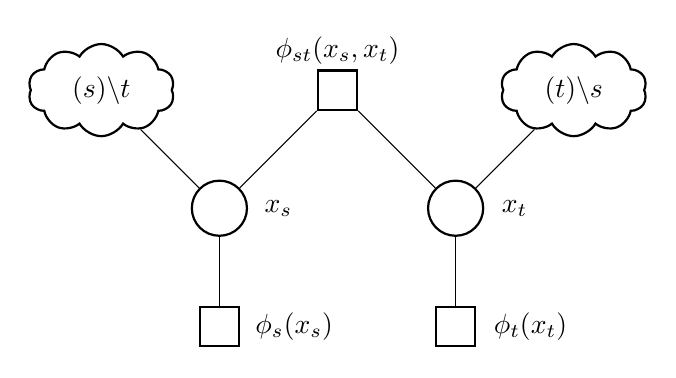
\begin{tikzpicture}
      % \tikzstyle{enode} = [thick, draw=blue, circle, inner sep = 3pt,
      % align=center]
      \tikzstyle{enode} = [thick, draw=black, circle, inner sep = 4pt, minimum size = 0.7cm, align=center]
      \tikzstyle{nnode} = [thick, rectangle, rounded corners = 0pt, minimum size = 0.5cm,draw,inner sep = 2pt]

      \tikzstyle{cnode} = [thick, cloud, draw,cloud puffs=10, cloud puff arc=120, aspect=2, inner ysep=4pt]

      \node[cnode] (pajk) at (3, 1.5) {$\Nn(t)\backslash s$};
      \node[cnode] (paik) at (-3, 1.5) {$\Nn(s)\backslash t$};

      \node[nnode] (tk) at (0, 1.5) {};
      \node[] at ($(tk) + (0, 0.5)$) {$\phi_{st}(x_s, x_t)$};
      \node[enode] (xi) at (-1.5 ,0) {};
      \node[] at ($(xi) + (0.75,0)$) {$x_s$};
      
      \node[nnode] (fi) at (-1.5 , -1.5) {};
      \node[] at ($(fi) + (0.95,0)$) {$\phi_s(x_s)$};
      

      \node[enode] (xj) at (1.5 ,0) {};
      \node[] at ($(xj) + (0.75,0)$) {$x_t$};
      
      \node[nnode] (fj) at (1.5 , -1.5) {};
      \node[] at ($(fj) + (0.95,0)$) {$\phi_t(x_t)$};
      
      % connections

      \draw[-] (xi) to (fi);
      \draw[-] (xi) to (tk);
      \draw[-] (xi) to (paik);

      \draw[-] (xj) to (fj);
      \draw[-] (xj) to (tk);
      \draw[-] (xj) to (pajk);
    \end{tikzpicture}
    \caption{Factor graph illustration of $p(\bm{x})$ in \eqref{eq:mrf}.}\label{fig:factor-graph}
  \end{centering}
\end{figure}


We consider a probability distribution over random vector $\bm{x} = \left(  x_1, x_2, \cdots,  x_N  \right)$, where $\bm{x} \in \bm{\Xx}$ and $\bm{\Xx}=\prod_{i=1}^N\Xx_i$. For explanation simplicity, we define that each domain is instantiated as the same discrete finite set $\Xx$, i.e., $\bm{\Xx}=\prod_{i=1}^N\Xx$ and $x_i \in \Xx$. Note $\alpha$-BP is applicable for the different domain setting $\bm{\Xx}=\prod_{i=1}^N\Xx_i$. Let us denote the undirected graph of a pairwise MRF by $\Gg:=(\Vv, \Ee)$. $\Vv=\left[ 1 : N \right]$ is the node set associated with the index set of entries of $\bm{x}$. The graph contains undirected edges $\Ee \subset \Vv \times \Vv$, where a pair of $(s, t) \in \Ee$ if and only if nodes $s$ and $t$ are connected by an edge. In addition to the undirected edge set, let us also define the directed edge set induced from $\Gg$ by $\vec{\Ee}$. We have $\abs{\vec{\Ee}} = 2\abs{\Ee}$, where $\abs{\cdot}$ denotes the carnality. These directed edges serve the purpose of convergence analysis only.



The joint distribution of $\bm{x}$ can be formulated as a pairwise factorization form in a pairwise MRF as
\begin{equation}\label{eq:mrf}
  p(\bm{x}) \propto \prod_{{s\in \Vv}} \phi_s(x_s) \prod_{(s,t) \in \Ee} \phi_{st}(x_s, x_t),
\end{equation}
where $\phi_{s}: \Xx \rightarrow (0, \infty)$ and $\phi_{st}: \Xx \times \Xx \rightarrow (0, \infty)$ are factor potentials. Here the normalization is omitted. Note the union of the node set and the edge set, i.e. $\Vv \cup \Ee$, instantiates the factor index set $\Ff$ of a general MRF in \eqref{chp2:eq:mrf-definition} here.

The factor graph representation of \eqref{eq:mrf} is shown in
Figure~\ref{fig:factor-graph}. In the figure, $\Nn(s)$ is the set of variable nodes neighboring $x_s$ via
pairwise factors, i.e. $\Nn(s) = \left\{ t|(t,s) \in \Ee \right\}$, and $\backslash$ denotes exclusion.

\subsection{From $\alpha$-divergence minimization to $\alpha$-BP}
We start with defining a surrogate distribution and then use the surrogate distribution to approximate a given distribution. The message passing rule of $\alpha$-BP is derived by solving the distribution approximation problem.

% \subsubsection{Fully Factorized Surrogate}
We begin with defining a distribution
\begin{equation}
  q(\bm{x}) \propto \prod_{{s\in \Vv}} \tilde{\phi}_s(x_s) \prod_{(s,t) \in \Ee} \tilde{\phi}_{st}(x_s, x_t),
\end{equation}
that is similarly factorized as the joint distribution $p(\bm{x})$. The distribution $q(\bm{x})$ acts as a surrogate distribution of $p(\bm{x})$. The surrogate distribution would be used to estimate inference problems of $p(\bm{x})$. We further choose $q(\bm{x})$ such that it can be fully factorized, which means that $\tilde{\phi}_{s,t}(x_s, x_t)$ can be factorized into product of two independent functions of $x_s, x_t$ respectively. We denote this factorization as
\begin{equation}
  \tilde{\phi}_{s,t}(x_s, x_t) := m_{st}(x_t) m_{ts}(x_s).
\end{equation}
We use the notation $m_{ts}(x_s)$ to denote the factor as a function of $x_s$. $m_{ts}: \Xx \rightarrow (0, \infty)$, serves as the message along directed edge $(t \rightarrow s)$ in our algorithm. Similarly we have factor or message $m_{st}(x_t)$. Then the marginal can be formulated straightforwardly as
\begin{equation}
  q_s(x_s) \propto \tilde{\phi}_s(x_s) \prod_{w\in \Nn(s)} m_{ws}(x_s).
\end{equation}

Now, we are going to use the heuristic scheme as in \eqref{eq:fixed-point-iter} to minimize the information loss by using a fully factorized $q(\bm{x})$ to represent $p(\bm{x})$. The information loss is measured by $\alpha$-divergence $\Dd_{\alpha}(p(\bm{x}) \| q(\bm{x}))$.


We perform a factor-wise refinement procedure to update the factors of $q(\bm{x})$ such that $q(\bm{x})$ approximates $p(\bm{x})$. This approach is similar to the factor-wise refinement procedure in assumed density filtering algorithm\cite{ghosh2016assumed, opper1999bayesian} and expectation propagation \cite{divergence-measures-and-message-passing,Minka:2001:EPA:647235.720257}. Without loss of generality, we begin to refine the factor $\tilde{\phi}_{ts}(x_t, x_s)$ via $\alpha$-divergence with its $\alpha$-parameter assignment as $\alpha_{ts}$. Define $q^{\backslash (t,s)}(\bm{x})$ as the product of all other factors excluding $\tilde{\phi}_{ts}(x_t, x_s)$
\begin{align}
  q^{\backslash (t,s)}(\bm{x})
  = q(\bm{x})/\tilde{\phi}_{ts}(x_t,
  x_s) \propto \prod_{{s\in \Vv}} \tilde{\phi}_s(x_s) \prod_{(v,u) \in
  \Ee\backslash (t,s)}
  \tilde{\phi}_{vu}(x_v, x_u).
  % &= \left(
  %   \tilde{\phi}_s(x_s) \prod_{w\in \Nn(s) \backslash t}m_{ws}(x_s)
  % \right)
  % \left(
  %   \tilde{\phi}_t(x_t) \prod_{w\in \Nn(t) \backslash s}m_{wt}(x_t)
  % \right)
  % \left(
  %   \prod_{v \in \Vv \backslash s,t}
  %   \tilde{\phi}_v(x_v) \prod_{w\in \Nn(v)}m_{wv}(x_v)
  % \right)\nonumber \\
\end{align}
We also exclude the factor $\phi_{ts}(x_t, x_s)$ in $p(\bm{x})$ to obtain $p^{\backslash (t,s)}(\bm{x})$. % Assume that we already have had $q^{\backslash (t,s)}(\bm{x})$ as a good approximation of $p^{\backslash (t,s)}(\bm{x})$, i.e. $q^{\backslash (t,s)}(\bm{x}) \approx p^{\backslash (t,s)}(\bm{x})$, where $\approx$ denotes approximately equality, it is $\tilde{\phi}_{ts}(x_t, x_s)$ that remains to be refined. In refining factor $\tilde{\phi}_{ts}(x_t, x_s)$ with $\alpha$-divergence under such assumption, the problem
Instead of updating $\tilde{\phi}_{ts}(x_t, x_s)$ directly by solving
\begin{equation}
  \!\!\!\uargmin{\tilde{\phi}_{ts}^{\mathrm{new}}(x_t, x_s)}\!\!\!\! \Dd_{\alpha_{ts}}\!\!\left(  p^{\backslash (t,s)}\!(\bm{x})\phi_{ts}(x_t, x_s)\|q^{\backslash (t,s)}\!(\bm{x})\tilde{\phi}_{ts}^{\mathrm{new}}(x_t, x_s)\right),
\end{equation}
we consider the following tractable problem
\begin{equation}\label{eq:alpha-minimize-factor}
  \!\!\!\uargmin{\tilde{\phi}_{ts}^{\mathrm{new}}(x_t, x_s)}\!\!\!\!
  \Dd_{\alpha_{ts}}\!\!\left( q^{\backslash (t,s)}\!(\bm{x}){\phi}_{ts}(x_t, x_s)
    \|q^{\backslash (t,s)}\!(\bm{x})\tilde{\phi}_{ts}^{\mathrm{new}}(x_t, x_s) \right),
\end{equation}
which searches for new factor $\tilde{\phi}_{ts}^{\mathrm{new}}(x_t, x_s)$ such $q$ can approximate $p$ better. In \eqref{eq:alpha-minimize-factor}, $\Dd_{\alpha_{ts}}(\cdot)$ denotes the $\alpha$-divergence with the parameter $\alpha_{ts}$. Note that the approximation \eqref{eq:alpha-minimize-factor} is accurate when $q^{\backslash (t,s)}(\bm{x})$ is equal to $p^{\backslash (t,s)}(\bm{x})$. 
Using fixed-point update in \eqref{eq:fixed-point-iter}, the problem in \eqref{eq:alpha-minimize-factor} is equivalent to
\begin{align}\label{eq:update-rule}
  q^{\backslash (t,s)}(\bm{x})\tilde{\phi}_{ts}^{\mathrm{new}}(x_t, x_s) \propto
  % &\propto \text{proj}\left[ \left( q^{\backslash (t,s)}(\bm{x}){\phi}_{ts}(x_t, x_s) \right)^{\alpha_{ts}} \left(q^{\backslash (t,s)}(\bm{x})\tilde{\phi}_{ts}(x_t, x_s)  \right)^{1-\alpha_{ts}} \right] \nonumber \\
  \mathrm{proj}\left[ q^{\backslash
  (t,s)}(\bm{x}){\phi}_{ts}(x_t, x_s)^{\alpha_{ts}} \tilde{\phi}_{ts}(x_t, x_s)^{1-\alpha_{ts}} \right]. 
\end{align}

Without loss of generality, we update $m_{ts}$ and define
\begin{equation}\label{eq:new_ts}
  \tilde{\phi}_{ts}^{\mathrm{new}}(x_t, x_s) = m_{ts}^{\mathrm{new}}(x_s) m_{st}(x_t).
\end{equation}
Since KL-projection onto a fully factorized distribution reduces to matching the marginals \cite[Proposition~8.3]{koller2009pgm}, substituting \eqref{eq:new_ts} into \eqref{eq:update-rule}, we obtain
\begin{align}\label{eq:message-update}
  \sum_{\bm{x}\backslash x_s} q^{\backslash (t,s)}(\bm{x}) \tilde{\phi}_{ts}^{\mathrm{new}}(x_t, x_s) 
  \propto \sum_{\bm{x}\backslash x_s} q^{\backslash (t,s)}(\bm{x}) \phi_{ts}(x_t, x_s)^{\alpha_{ts}} \tilde{\phi}_{ts}(x_t, x_s)^{1-\alpha_{ts}}.
\end{align}
Solving \eqref{eq:message-update} gives the message passing rule as
\begin{align}\label{eq:message-rule-pairwise}
  {m}^{\text{new}}_{ts}(x_s) \propto  m_{ts}(x_s)^{1-\alpha_{ts}} \bigg[\sum_{x_t} \phi_{ts}(x_t, x_s)^{\alpha_{ts}} {m}_{st}(x_t)^{1-\alpha_{ts}}\tilde{\phi}_t(x_t) \prod_{w\in \Nn(t)\backslash s}m_{wt}(x_t) \bigg].
\end{align}

As for the singleton factor $\tilde{\phi}_t(x_t)$, we can do the refinement procedure on $\tilde{\phi}_t(x_t)$ in the same way as we have done on $\tilde{\phi}_{ts}(x_t, x_s)$. This gives us the update rule of $\tilde{\phi}_t(x_t)$ as
\begin{equation}\label{eq:fix-factor-update}
  \tilde{\phi}_t^{\mathrm{new}}(x_t) \propto \phi_t(x_t)^{\alpha_{t}} \tilde{\phi}_t(x_t)^{1-\alpha_{t}},
\end{equation}
which is the belief from factor $\phi_t(x_t)$ to variable $x_t$. Here $\alpha_t$ is the local assignment of parameter $\alpha$ in $\alpha$-divergence in the refining factor $\tilde{\phi}_t(x_t)$. Note, if we initialize $\tilde{\phi}_t(x_t) = \phi_t(x_t)$, then it remains the same in all iterations, which makes
\begin{align}\label{eq:message-rule}
  {m}^{\mathrm{new}}_{ts}(x_s) \propto
  m_{ts}(x_s)^{1-\alpha_{ts}} \bigg[\sum_{x_t} \phi_{ts}(x_t, x_s)^{\alpha_{ts}} {m}_{st}(x_t)^{1-\alpha_{ts}} {\phi}_t(x_t) \prod_{w\in \Nn(t)\backslash s}m_{wt}(x_t) \bigg].
\end{align}
In our notations, a factor potential is undirected, i.e. $\phi_{ts}(x_t, x_s)=\phi_{st}(x_s, x_t)$ for all $(t,s) \in \Ee$. When refining factors with $\alpha$-BP, each factor potential (corresponding to an edge of $\Gg$) can be associated with a difference setting of $\alpha$ value. In addition we also have $\alpha_{ts} = \alpha_{st}$.

\section{Remarks on $\alpha$ Belief Propagation}\label{subsec:remark}

As discussed in Section~\ref{chpt3:sec:alpha-divergence}, $\mathrm{KL}(p\|q)$ is the special case of $\Dd_{\alpha}(p\|q)$ when $\alpha \rightarrow 1$. When restricting $\alpha_{st}=1$ for all $(s,t) \in \Ee$, the message-passing rule in \eqref{eq:message-rule} becomes
\begin{equation}\label{chpt3:eq:bp-update-rule}
  {m}^{\text{new}}_{ts}(x_s) \propto 
  \sum_{x_t} \phi_{st}(x_s, x_t) {\phi}_t(x_t) \prod_{w\in \Nn(t)\backslash s}m_{wt}(x_t),
\end{equation}
which is exactly the messages of standard BP \cite{Bishop:2006:PRM:1162264}. From this point of view, we can say $\alpha$-BP is a generalization of BP. Additionally, the BP update rule in \eqref{chpt3:eq:bp-update-rule} actually corresponds to the fixed-point iteration assignment by solving the Bethe free energy minimization problem in \eqref{chpt2:bethe-free-energy}.


Note although the mean field method also uses fully-factorized approximation, it is obtained differently from $\alpha$-BP and its factorization differs from that of $\alpha$-BP. From another perspective, mean field methods are actually using information projections from $p(\bm{x})$ to a fully-factorized space via KL divergence as explained in Section~\ref{chpt2:sec:variational-inference}.
In addition, $\alpha$-BP is different from standard BP with damping technique. The latter case uses a message update rule that differs from \eqref{chpt3:eq:bp-update-rule} slightly in the way of assigning updated messages. 


Additionally, $\alpha$-BP differs from the tree-reweighted belief propagation \cite{wainwright2008graphical} in the way of message update rule and also how algorithm is derived. 
The tree-reweighted BP shares some similarity with $\alpha$-BP in the formula of the message-passing rule, namely, the pairwise log-potential functions are scaled by a weight and reweighted old messages appear in the computation of new messages. But different from $\alpha$-BP, tree-reweighted BP is derived by obtaining an upper bound of log-partition function of $p(\bm{x})$ first via a Jensen's inequality and minimize the upper bound. The upper bound is
\begin{align}
  F_T(q) =& \sum_{s\in\Vv}\sum_{x_s}q_s(x_s) \ln{\frac{q_s(x_s)}{\phi_s(x_s)}}  + \sum_{(s,t)\in\Ee}\mu_{st}\sum_{x_s, x_t} q_{st}(x_s, x_t) \ln\frac{q_{st}(x_s,x_t)}{q_s(x_s)q_t(x_t)} \nonumber \\
          & - \sum_{(s,t)\in\Ee}\sum_{x_s, x_t} q_{st}(x_s, x_t)\ln{\phi_{st}(x_t, x_t)},
\end{align}
where $0\leq \mu_{st} \leq 1$ is defined as the appearance probability of edge $(s, t) \in \Ee$, which denotes the appearance rate of edge $(s,t)$ among all spanning trees of graph $\Gg$. Denote the set of all spanning trees of $\Gg$ by $\Tt(\Gg)$. $\mu_{st}$ is the probability that edge $(s,t)$ exists in a randomly selected spanning tree from $\Tt(\Gg)$. The appearance rate can be expensive to compute as it is defined on all spanning trees of a graph.


The upper bound $F_T$ can be reduced into the Bethe free energy \eqref{chpt2:bethe-free-energy} when $\mu_{st}=1$, $\forall ~(s,t)\in \Ee$. The message-passing updates of the tree-reweighted algorithm corresponds to the minimization of $F_T$ with marginalization constraints, which can be written as
\begin{align}
  {m}^{\text{new}}_{ts}(x_s) \propto \sum_{x_t} \phi_{st}(x_s, x_t)^{1/\mu_{st}} {\phi}_t(x_t) \frac{\prod_{w\in \Nn(t)\backslash s}m_{wt}(x_t)^{\mu_{wt}} }{m_{st}(x_t)^{1-\mu_{st}}}.
\end{align}
In the message update rule, both pairwise potential factor and old messages are reweighted, which are different from the way of how pairwise potential factor and old message are reweighted in message update in \eqref{eq:message-rule}. Nevertheless, $\alpha$-BP is derived in a way that is different from tree-reweighted BP.

\begin{figure}[!t]
  \begin{centering}
    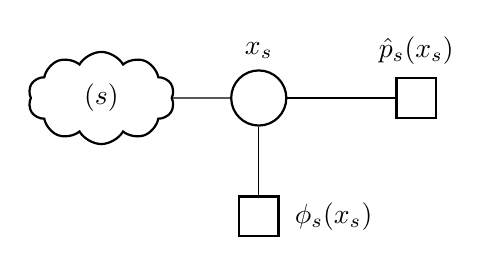
\begin{tikzpicture}
      \tikzstyle{enode} = [thick, draw=black, circle, inner sep = 4pt, minimum size = 0.7cm, align=center]
      \tikzstyle{nnode} = [thick, rectangle, rounded corners = 0pt, minimum size = 0.5cm,draw,inner sep = 2pt]

      \tikzstyle{cnode} = [thick, cloud, draw,cloud puffs=10, cloud puff arc=120, aspect=2, inner ysep=4pt]

      \node[cnode] (paik) at (-2, 0) {$\Nn(s)$};
      \node[enode] (xi) at (0 ,0) {};
      \node[] at ($(xi) + (0,0.6)$) {$x_s$};

      \node[nnode] (fi) at (0 , -1.5) {};
      \node[] at ($(fi) + (0.95, 0)$) {$\phi_s(x_s)$};

      \node[nnode] (pi) at (2, 0) {};
      \node[] at ($(pi) + (0, 0.6)$) {$\hat{p}_s(x_s)$};
      % connections
      \draw[-] (xi) to (fi);
      \draw[-] (xi) to (pi);
      \draw[-] (xi) to (paik);
    \end{tikzpicture}
    \caption{Modified graphical model with prior factor.}\label{fig:factor-graph-with-prior}
  \end{centering}
\end{figure}


From the practical perspective, $\alpha$-BP as a meta algorithm can be used with other methods in a hybrid way. Inspired by \cite{pseudo_priorBP2010} and assembling methods \cite{James:2014:ISL:2517747}, we can modify the graphical model shown in Figure~\ref{fig:factor-graph} by adding an extra factor potential $\hat{p}_s(x_s)$ to each $x_s$. The extra factor potential $\hat{p}_s(x_s)$ acts as prior information that can be obtained from other methods. In other words, this factor potential stands for our belief from exterior estimation. Then we can run our $\alpha$-BP on the modified graph. The modified graph is shown in Figure~\ref{fig:factor-graph-with-prior}.

% We summarize the $\alpha$-BP into the pseudo-code in Algorithm~\ref{alg:alphaBP}.

% \begin{algorithm}[tb]
%   \caption{Algorithm of $\alpha$-BP}\label{alg:alphaBP}
%   \begin{algorithmic}
%     \STATE {\bfseries Input:} Graphic model of $p(\bm{x})$
%     \STATE Initialize $q(\bm{x})$
%     \IF {Prior belief on $x_i$ available}
%     \STATE Add prior factor as Figure~\eqref{fig:factor-graph-with-prior}
%     \ENDIF
%     \REPEAT
%     \FOR {each directed edge $(t \rightarrow s)$ of graph model of $p(\bm{x})$}
%     \STATE Message passing by \eqref{eq:message-rule} (or
%     \eqref{eq:message-rule-pairwise}, \eqref{eq:fix-factor-update} if $\tilde{\phi}_s(x_s)$ is not initialized as $\phi_s(x_s)$)
%     \ENDFOR
%     \UNTIL{Converge or maximum number of iteration reached.}
%   \end{algorithmic}
% \end{algorithm}


\section{Convergence of $\alpha$-BP with a Binary State Space}\label{chpt3:sec:cnvg-thm}

As pointed earlier, a key issue of BP and its variants is whether and when they converge. In this section, we discuss when $\alpha$-BP converges. 
From the high-level perspective, we are going to use \textit{contraction} property to show when $\alpha$-BP does converge.
\begin{definition}\label{chpt3:def:contraction}
  For a number $c \in [0,1)$, an operator $G$ over a metric space $(\Delta, d(,))$ is $c$-contraction relative to the distance function $d(,)$ if for any $\bm{z}, \bm{z}^{\prime} \in \Delta$, we have
  \begin{equation}
    d(G(\bm{z}), G(\bm{z}^{\prime})) \leq c d(\bm{z}, \bm{z}^{\prime}).
  \end{equation}
\end{definition}
Definition~\ref{chpt3:def:contraction} tells us that an operator is a contraction if its application to two points in the space is guaranteed to decrease the distance between them by at least a constant $c < 1$. \textit{Thus, we essentially are going to show that the message update rule of $\alpha$-BP is actually a contraction, under which condition we would show that $\alpha$-BP converges}.

We consider the case of binary $\Xx$ with $\Xx=\left\{ -1, 1 \right\}$, to gain insights into the convergence behavior of $\alpha$-BP. The factor potentials are further detailed as
\begin{align}
  \phi_{st}(x_s, x_t) &= \exp\left\{ \theta_{st}(x_s, x_t)\right\}, \nonumber \\
  \phi_{s}(x_s) &= \exp\left\{ \theta_{s}(x_s) \right\}.
\end{align}
Further assume the symmetric property of potentials
\begin{align}\label{chpt3:eq:symmetric-prop}
  \theta_{ts}(x_t, x_s) &= -\theta_{ts}(x_t, -x_s) = -\theta_{ts}(-x_t, x_s), \nonumber\\
  \theta_{s}(x_s) &= - \theta_s(-x_s).
\end{align}

\begin{example}
  The Ising model, from statistical physics \cite{ising1925, PhysRev.65.117}, is such a model whose potentials fulfill the symmetric property in \eqref{chpt3:eq:symmetric-prop}. In the graph $\Gg = (\Vv, \Ee)$ of an Ising model, the random variable $x_s$ takes the spin value $\left\{ -1, +1 \right\}$. The values of $\bm{x}$ associated with the nodes of $\Gg$ might represent the orientations of magnets in a field or the states of particles of gas in the context of statistical physics. Two elements $x_t$ and $x_s$ of $\bm{x}$ are allowed to interact directly only if there is an edge between them directly, i.e., $(t, s) \in \Ee$. The potential factors of an Ising model is in exponential family. This leads the joint distribution
  \begin{equation*}
    p(\bm{x};\bm{\theta}) \propto \exp\left\{ \sum_{s\in \Vv} b_s x_s + \sum_{(t, s) \in \Ee} J_{ts} x_t x_s \right\},
  \end{equation*}
  the factors of which fulfill the symmetric property in \eqref{chpt3:eq:symmetric-prop}.
\end{example}

For notation simplicity, we use $\theta_{ts}=\theta_{ts}(1, 1)$ and $\theta_s = \theta_s(1)$. Denote by $\bm{\alpha}$ the vector of all local assignments of parameter $\alpha$, i.e. $\bm{\alpha} = \left(  \alpha_{ts} \right)_{(t ,s) \in \Ee }$, by $\bm{\theta}$ the vector of all parameters of the potentials, i.e. $\bm{\theta} = \left(  \theta_{ts} \right)_{(t ,s) \in \Ee }$.  Define a matrix $\bm{M}(\bm{\alpha}, \bm{\theta})$ of size $\abs{\vec{\Ee}} \times \abs{\vec{\Ee}}$, in which its entries are indexed by directed edges $(t\rightarrow s)$, as
\begin{align}\label{eq:matrix_m}
  M_{(t\rightarrow s), (u \rightarrow v)} =
  \begin{cases}
    \abs{ 1 - \alpha_{ts}}, &\quad u=t, v=s, \\
    \abs{ 1 - \alpha_{ts}} \tanh \abs{\alpha_{ts} \theta_{ts}}, & \quad u = s, v =t, \\
    \tanh\abs{\alpha_{ts} \theta_{ts}}, & \quad u \in \Nn(t)\backslash s, v = t, \\
    0, & \quad \mathrm{otherwise}.
  \end{cases}
\end{align}
\begin{theorem}\label{thm:normd}
  For an arbitrary pairwise Markov random field over binary variables,
  if the largest singular value of matrix $\bm{M}(\bm{\alpha}, \bm{\theta})$ is less than one,
  $\alpha$-BP converges to a fixed point. The associated fixed point is unique.
\end{theorem}

\begin{proof}
  Let us define $z_{ts}$ as the log ratio of belief from node $t$ to node $s$ on two states of $\Xx$, i.e.
  \begin{equation}\label{eq:log-ratio-uv}
    z_{ts} = \log\frac{m_{ts}(1)}{m_{ts}(-1)}.
  \end{equation}

  By combining the local message passing rule in \eqref{eq:message-rule} with \eqref{eq:log-ratio-uv}, we obtain a local update function $F_{ts}: \; \RR^{\abs{\vec{\Ee}}} \rightarrow \RR$ that maps $\bm{z} = \left( z_{ts} \right)_{(t \rightarrow s) \in \Ee}$ to updated $z_{ts}$, which can be expressed as
  % Substituting \eqref{eq:message-rule} into \eqref{eq:log-ratio-uv} gives
  % \begin{align}
      %       &F_{ts}(\bm{z}) = (1- \alpha_{ts})z_{ts} + \\
      %               &\log\frac{\exp\left\{ \alpha_{ts}\left[ \theta_{ts}(1,1) - \theta_{ts}(-1,1) \right] + \theta_t(1) - \theta_t(-1) + (1 - \alpha_{ts})z_{st} + \sum_{w\in \Nn(t)\backslash s} z_{wt} \right\}+1}
                        %                         {\exp\left\{ \alpha_{ts}\left[ \theta_{ts}(1,-1) - \theta_{ts}(-1,1) \right] + \theta_t(1) - \theta_t(-1) + (1 - \alpha_{ts})z_{st} + \sum_{w\in \Nn(t)\backslash s} z_{wt} \right\} +
                        %                         \exp\left\{ \alpha_{ts}\left[ \theta_{ts}(-1,-1) - \theta_{ts}(-1,1) \right] \right\}},
                        %     \end{align}
                        %                         where $\bm{z}$ is vector with element entry $z_{vu}, v,u \in \Vv$.
                        %                         With the symmetric property, the log ratio updates for $z_{ts}$ can be reduced as
  \begin{equation}\label{eq:ratio-update}
    F_{ts}(\bm{z}) = (1-\alpha_{ts}) z_{ts} + f_{ts}(\bm{z}),
  \end{equation}
  where
  \begin{equation}
    f_{ts}(\bm{z}) = \log\frac{\exp\left\{ 2 \alpha_{ts} \theta_{ts} + \Delta_{ts}(\bm{z}) \right\}+1}
    {\exp\left\{ \Delta_{ts}(\bm{z}) \right\} +
      \exp\left\{ 2 \alpha_{ts} \theta_{ts} \right\}},
  \end{equation}
  with
  \begin{equation}
    \Delta_{ts}(\bm{z}) = 2 \theta_s + (1 - \alpha_{ts}) z_{st} + \sum_{w\in \Nn(u)\backslash t} z_{wt}.
  \end{equation}

  In the following, we use superscript ${(n)}$ to denote the $n$-th iteration. Since $f_{ts}$ is continuous on $\RR^{\abs{\vec{\Ee}}}$ and differentiable, we have
  \begin{align}\label{eq:ratio_diff_at_n}
    & z_{ts}^{(n+1)} - z_{ts}^{(n)} \nonumber \\
    =& (1-\alpha_{ts}) (z_{ts}^{(n)} - z_{ts}^{(n-1)}) + f_{ts}(\bm{z}^{(n)}) - f_{ts}(\bm{z}^{(n-1)}) \nonumber \\
    \overset{(a)}{=}& (1-\alpha_{ts}) (z_{ts}^{(n)} - z_{ts}^{(n-1)}) + \nabla f_{ts}(\bm{z}^{\lambda})^{T} (\bm{z}^{(n)} - \bm{z}^{(n-1)}),
  \end{align}
  where $(a)$ follows by the mean-value theorem, $\bm{z}^{\lambda} = \lambda \bm{z}^{(n)} + (1 - \lambda) \bm{z}^{(n-1)}$ for some $\lambda \in (0,1)$, and $\nabla f_{ts}(\bm{z}^{\lambda})$ denotes the gradient of $f_{ts}$ evaluated at $\bm{z}^{\lambda}$. In further details, $\nabla f_{ts}$ is given by
  \begin{equation}\label{eq:F_pd}
    \pd{f_{ts}}{z}=
    \begin{cases}
      ( 1 - \alpha_{ts}) \pd{f_{ts}}{\Delta_{ts}}, &\quad z = z_{st}, \\
      \pd{f_{ts}}{\Delta_{ts}}, &\quad z = z_{wt}, w\in N(t)\backslash s. \\
      0, &\quad \mathrm{otherwise}.  \\
    \end{cases}
  \end{equation}
  
  Our target here is to find the condition to make sequence $\left( z_{ts}^{(n+1)} - z_{ts}^{(n)} \right)$ to converge. To this aim we need to bound the term $\nabla f_{ts}(\bm{z}^{\lambda})^{T} (\bm{z}^{(n)} - \bm{z}^{(n-1)})$ in \eqref{eq:ratio_diff_at_n}. For this purpose, we need two auxiliary functions $H, G: \RR^2 \rightarrow \RR$ from Lemma~$4$ in \cite{roosta2008reweighed_sum_product}, which are given in the following for completeness,
  \begin{align}
    H(\mu; \kappa) &:= \log \frac{\exp(\mu + \kappa) +1}{\exp(\mu) + \exp(\kappa)}, \nonumber \\
    G(\mu; \kappa) &:= \frac{\exp(\mu + \kappa)}{\exp(\mu + \kappa) + 1} - \frac{\exp(\mu)}{\exp(\mu) + \exp(\kappa)} \nonumber \\
                   &= \frac{\sinh{\kappa}}{\cosh{\kappa} + \cosh{\mu}},
  \end{align}
  where it holds that $\pd{H(\mu; \kappa)}{\mu} = G(\mu; \kappa)$. Further, it holds that
  $\abs{G(\mu; \kappa)} \leq \abs{G(0, \kappa)} = \tanh(\abs{\kappa}/2)$.
  Then we have
  \begin{align}\label{eq:eqv_aux_functions}
    f_{ts}(z) &= H(\Delta_{ts}(\bm{z}) ;2 \alpha_{ts} \theta_{ts}), \nonumber \\
    \pd{f_{ts}}{\Delta_{ts}} &= G(\Delta_{ts}(\bm{z}) ;2 \alpha_{ts} \theta_{ts}),
  \end{align}
  which implies
  \begin{equation}\label{eq:f-bound}
    \bigg|{\pd{f_{ts}}{\Delta_{ts}}}\bigg| \leq \tanh(\abs{\alpha_{ts}\theta_{ts}}).
  \end{equation}
  Combining \eqref{eq:ratio_diff_at_n}, \eqref{eq:F_pd}, \eqref{eq:eqv_aux_functions} and \eqref{eq:f-bound}, we have
  \begin{align}\label{eq:ratio_cvg_step}
    &\abs{z_{ts}^{(n+1)} - z_{ts}^{(n)}} \nonumber\\
    & = \abs{(1-\alpha_{ts}) (z_{ts}^{(n)} - z_{ts}^{(n-1)}) + \nabla f_{ts}(\bm{z}^{\lambda})^{T} (\bm{z}^{(n)} - \bm{z}^{(n-1)})} \nonumber \\
    & \leq \abs{(1-\alpha_{ts}) (z_{ts}^{(n)} - z_{ts}^{(n-1)})} + \abs{\nabla f_{ts}(\bm{z}^{\lambda})^{T} (\bm{z}^{(n)} - \bm{z}^{(n-1)})} \nonumber \\
    & = \abs{ 1 - \alpha_{ts}} \abs{z_{ts}^{(n)} - z_{ts}^{(n-1)}} + \abs{\nabla f_{ts}(\bm{z}^{\lambda})}^{T} \abs{\bm{z}^{(n)} - \bm{z}^{(n-1)}} \nonumber \\
    & \overset{(a)}{\leq} \abs{ 1 - \alpha_{ts}} \abs{z_{ts}^{(n)} - z_{ts}^{(n-1)}} + \abs{ 1 - \alpha_{ts}} \tanh(\abs{\alpha_{ts} \theta_{ts}}) \abs{z_{st}^{(n)} - z_{st}^{(n-1)}} \nonumber \\
    &+ \sum_{w\in N(t)\backslash s} \tanh(\abs{\alpha_{ts} \theta_{ts}}) \abs{z_{wt}^{(n)} - z_{wt}^{(n-1)}},
  \end{align}
  where step $(a)$ holds by applying \eqref{eq:F_pd} and \eqref{eq:f-bound}.

  
  Concatenating all $(t\rightarrow s) \in \vec{\Ee}$ for inequality \eqref{eq:ratio_cvg_step} gives
  \begin{equation}\label{eq:ratio-update-ineq}
    \abs{\bm{z}^{(n+1)} - \bm{z}^{n}} \leq \bm{M}(\alpha, \bm{\theta})\abs{\bm{z}^{(n)} - \bm{z}^{(n-1)}},
  \end{equation}
  where $\bm{M}(\bm{\alpha}, \bm{\theta})$ is defined in \eqref{eq:matrix_m}, and $\leq$ in \eqref{eq:ratio-update-ineq} denotes the element-wise inequality. Also note that in \eqref{eq:ratio-update-ineq}, the $\abs{\cdot}$ operator on a vector is a bit abused and denotes the element-wise absolute operation on the vector. From \eqref{eq:ratio-update-ineq}, we could further have
  \begin{align}\label{eq:ine-normp-iteration}
    \norm{\bm{z}^{(n+1)} - \bm{z}^{n}}_{p} &\leq \norm{\bm{M}(\alpha, \bm{\theta})\abs{\bm{z}^{(n)} - \bm{z}^{(n-1)}}}_{p},               
  \end{align}
  where $1\leq p < \infty$, and $\norm{\cdot}_p$ denotes the ${\ell}^p$-norm.

  When applying $p=2$ to \eqref{eq:ine-normp-iteration}, we have
  \begin{align}\label{eq:ieq-largest-singular}
    \normd{\bm{z}^{(n+1)} - \bm{z}^{(n)}} &\leq \normd{\bm{M}(\bm{\alpha}, \bm{\theta})\abs{\bm{z}^{(n)} - \bm{z}^{(n-1)}}} \nonumber \\
                                          &\leq \lambda^{\ast}(\bm{M})\normd{\bm{z}^{(n)} - \bm{z}^{(n-1)}},
  \end{align}
  where $\lambda^{\ast}(\bm{M})$ denotes the largest singular value of matrix
  $\bm{M}(\bm{\alpha}, \bm{\theta})$. If the largest singular value of $\bm{M}$ is less than $1$, the sequence
  $\left( \abs{\bm{z}^{(n+1)} - \bm{z}^{(n)}}\right)$ converges to zero in $\ell^2$-norm as $n \rightarrow \infty$. Therefore, for $\lambda^{\ast}(\bm{M})<1$, $\ell^2$-norm $\left(  \bm{z}^{(n)}  \right)$ is a Cauchy sequence and must converge. 

  By concatenating local update function \eqref{eq:ratio-update}, we have a global update function $\bm{F} = \left(  F_{ts}  \right)_{ (t \rightarrow s) \in \vec{\Ee}}$, which defines a mapping from $\RR^{\abs{\vec{\Ee}}}$ to $\RR^{\abs{\vec{\Ee}}}$. $\bm{F}$ is a continuous function of $\bm{z}$, and we have
  \begin{equation}
    \bm{F}(\lim_{n\rightarrow \infty}\bm{z}^{(n)}) = \lim_{n\rightarrow \infty}\bm{F}(\bm{z}^{(n)}).
  \end{equation}
  Assume that $\left(  \bm{z}^{(n)} \right)$ converges to
  $\bm{z}^{\ast}$. Then
  \begin{align}
    \bm{F}(\bm{z}^{\ast}) - \bm{z}^{\ast}
    &= \lim_{n\rightarrow \infty} \bm{F}(\bm{z}^{(n)}) -\lim_{n\rightarrow
      \infty} \bm{z}^{(n)} \nonumber \\
    &= \lim_{n\rightarrow \infty} (\bm{z}^{(n+1)} - \bm{z}^{(n)}) \nonumber \\
    &= 0.
  \end{align}
  Thus $\bm{z}^{\ast}$ must be a fixed point.

  In what follows we show that the fixed point is unique when $\lambda^{\ast}(\bm{M})<1$. Assume that there are two fixed points $\bm{z}_0^{\ast}$ and $\bm{z}_1^{\ast}$ for sequence $\left\{ \bm{z}^{(n)} \right\}$. Then we have
  \begin{align}\label{eq:two-fix-point}
    \bm{F}(\bm{z}_0^{\ast}) &= \bm{z}_0^{\ast}, \nonumber\\
    \bm{F}(\bm{z}_1^{\ast}) &= \bm{z}_1^{\ast}. 
  \end{align}
  Applying \eqref{eq:ieq-largest-singular} gives
  \begin{equation}\label{eq:two-fix-ineq}
    \normd{\bm{F}(\bm{z}_0^{\ast}) - \bm{F}(\bm{z}_1^{\ast})} \leq
    \lambda^{\ast}(\bm{M})\normd{\bm{z}_0^{\ast} - \bm{z}_1^{\ast}}.
  \end{equation}
  Substituting \eqref{eq:two-fix-point} into \eqref{eq:two-fix-ineq}
  gives
  \begin{equation}
    \normd{\bm{z}_0^{\ast} - \bm{z}_1^{\ast}} \leq
    \lambda^{\ast}(\bm{M})\normd{\bm{z}_0^{\ast} - \bm{z}_1^{\ast}},
  \end{equation}
  which gives us $\bm{z}_0^{\ast} = \bm{z}_1^{\ast}$ for $\lambda^{\ast}(\bm{M})<1$ and completes the uniqueness of the fixed point.
\end{proof}

\begin{remark}
  From Theorem~\ref{thm:normd} we can see that the sufficient condition for convergence of $\alpha$-BP is $\lambda^{\ast}(\bm{M}(\bm{\alpha}, \bm{\theta})) < 1$. It is interesting to notice that $\lambda^{\ast}(\bm{M}(\bm{\alpha}, \bm{\theta}))$ is a function of $\bm{\alpha}$ from $\alpha$-divergence and $\bm{\theta}$ from joint distribution $p(\bm{x})$. This means that whether $\alpha$-BP can converge depends on the graph $\Gg= (\Vv, \Ee)$ representing the problem $p(\bm{x})$ and also the choice of $\bm{\alpha}$. Therefore, proper choice of $\bm{\alpha}$ can guarantee the convergence of $\alpha$-BP if the sufficient condition can possibly be achieved for given $\bm{\theta}$.
\end{remark}

\begin{remark}
  The condition in Theorem~\ref{thm:normd} tells if $\alpha$-BP converges to a fixed point. However, it does not guarantee if the converged fixed point is a global optimum. Error analysis of BP and its variant is a challenging task. We discussed that the exact inference of BP in tree-structured graphs in Section~\ref{chpt2:sec:inference-mp}. The global optimum of the loopy BP algorithm can be guaranteed in rare cares. For instance, a ferromagnetic Ising model in which neighbors prefer to be in aligned states can get guaranteed global optimum with loopy BP\cite{frederic2019fast}. A successful application of (loopy) BP with bounded errors lies in coding theory, e.g., running a BP decoder on a graph whose structure (degrees of nodes) fulfills certain constraints can have its error bounded \cite{richardson2001}\cite[Section~7.2]{richardson2008}. 
\end{remark}

Given the fact that $\alpha$-BP would converge if the condition in Theorem~\ref{thm:normd} is fulfilled, the largest singular value computation for large-sized graph could be nontrivial. We give alternative sufficient conditions for the convergence of $\alpha$-BP.

\begin{corollary}\label{chpt3:cor:converge}
  $\alpha$-BP converges to a fixed point if the condition
  \begin{align}\label{chpt3:cor:choose-col}
    \umax{u \rightarrow v}  \abs{1-\alpha_{uv}} + \abs{1-\alpha_{vu}}\tanh{(\abs{\alpha_{vu} \theta_{vu}})} + \sum_{w \in \Nn(v) \backslash u} \tanh{(\abs{\alpha_{{vw}} \theta_{vw}})} < 1,
  \end{align}
  is fulfilled or the condition
  \begin{align}\label{chpt3:cor:choose-row}
    \umax{t \rightarrow s} \abs{1-\alpha_{ts}} (1 + \tanh(\abs{\alpha_{ts} \theta_{ts}})) + (\abs{\Nn(t)}-1)\tanh(\abs{\alpha_{ts} \theta_{ts}}) < 1.
  \end{align}
  is satisfied, where $\abs{\Nn(t)}$ denotes the carnality of the set $\Nn(t)$. The associated fixed point is unique.
\end{corollary}

\begin{proof}
  Setting $p=1$ to \eqref{eq:ine-normp-iteration}, we have
  \begin{equation}
    \normu{\bm{z}^{(n+1)} - \bm{z}^{n}} \leq \normu{\bm{M}(\alpha, \bm{\theta})(\bm{z}^{(n)} - \bm{z}^{n-1})}.
  \end{equation}
  Furthermore, from \eqref{eq:ine-normp-iteration}, we also have
  \begin{equation}
    \normi{\bm{z}^{(n+1)} - \bm{z}^{n}} \leq \normi{\bm{M}(\alpha, \bm{\theta})(\bm{z}^{(n)} - \bm{z}^{n-1})},
  \end{equation}
  where $\norm{\cdot}_{\infty}$ denotes the $\ell^{\infty}$-norm.
  Then we have
  \begin{align}\label{eq:row-col-norm-ineq}
    \normu{\bm{z}^{(n+1)} - \bm{z}^{n}} &\leq \normu{\bm{M}}\normu{(\bm{z}^{(n)} - \bm{z}^{n-1})}, \nonumber \\
    \normi{\bm{z}^{(n+1)} - \bm{z}^{n}} &\leq \normi{\bm{M}}\normi{(\bm{z}^{(n)} - \bm{z}^{n-1})},
  \end{align}
  where we omit the parameters of $\bm{M}$ here for simplicity. We can expand the first multiplicand on the right hand side of \eqref{eq:row-col-norm-ineq} as follows
  \begin{align}
    \normu{\bm{M}} =& \umax{u \rightarrow v}{\sum_{t\rightarrow s} M_{(t\rightarrow s), (u\rightarrow v)}} \nonumber \\
    =& \umax{u \rightarrow v}\abs{1-\alpha_{uv}} + \abs{1-\alpha_{vu}}\tanh{\abs{\alpha_{vu} \theta_{vu}}} + \sum_{w\in \Nn(v) \backslash u} \tanh{\abs{\alpha_{{vw}} \theta_{vw}}}, \nonumber \\
    \normi{\bm{M}} =& \umax{t \rightarrow s}{\sum_{u\rightarrow v} M_{(t\rightarrow s), (u\rightarrow v)}} \nonumber \\
    =& \umax{t \rightarrow s} \abs{1-\alpha_{ts}} (1 + \tanh\abs{\alpha_{ts} \theta_{ts}}) + (\abs{\Nn(t)}-1)\tanh\abs{\alpha_{ts} \theta_{ts}}.
  \end{align}
  When condition $\normu{\bm{M}} < 1$ is met, sequence $\left( \abs{\bm{z}^{(n+1)} - \bm{z}^{n}} \right)$ approaches to zero as $n\rightarrow \infty$. Similarly, condition $\normi{\bm{M}}<1$ can also guarantee the convergence to zero of sequence $\left( \abs{\bm{z}^{(n+1)} - \bm{z}^{n}} \right)$. The analysis for uniqueness of converged fixed point is similar to that in proof of Theorem~\ref{thm:normd}.
\end{proof}
\begin{remark}[Interpretation to the Results]
  
  Both Theorem~\ref{thm:normd} and Corollary~\ref{chpt3:cor:converge} offer sufficient conditions for convergence of $\alpha$-BP to a unique fixed point. The obtained results allow us to check if applying $\alpha$-BP in a certain configuration guarantees convergence without running the algorithm practically to try out, which saves computation resources when problems are at scales. To test the fulfillment of the conditions, the first step it to convert a problem to be solved into its pairwise MRF representation $\Gg(\Vv, \Ee)$. Secondly, construct the matrix $\bm{M}$ according to \eqref{eq:matrix_m}. Note the undirected edge set $\Ee$ of $\Gg$ is used to construct a directed edge set $\vec{\Ee}$ by assigning $(s\rightarrow t)$ and $(t\rightarrow s)$ with the same potential factor $\phi_{st}$ of $\Gg$. Thirdly, the condition fulfillment can be check by computing the largest singular value $\lambda^{\ast}(\bm{M})$ and testing $\lambda^{\ast}(\bm{M}) < 1$ as stated in Theorem~\ref{thm:normd}. Fulfilling this condition is to say that $\alpha$-BP is guaranteed to converge in the current setting.

  The size of the constructed matrix $\bm{M}$ is $\abs{\vec{\Ee}} \times \abs{\vec{\Ee}}$. $\bm{M}$ could be pretty large if a graph $\Gg$ is large or dense, which might cast the computation issue of the largest singular value of this matrix. In this case, Corollary~\ref{chpt3:cor:converge} offers the conditions to avoid the computation of the largest singular value. To be specific, after constructing the matrix \eqref{eq:matrix_m}, Corollary~\ref{chpt3:cor:converge} allows column-wise tests of $\bm{M}$, i.e., the column value of matrix $\bm{M}$ returning the largest quantity according to \eqref{chpt3:cor:choose-col} should be smaller than $1$ to guarantee the convergence of $\alpha$-BP. Note for a column $(u\rightarrow v)$, the elements of $\bm{M}$ involved in the testing computation are the factors corresponding to edges connected to node $v$ in $\Gg$. Alternatively, row-wise test can be carried out according to \eqref{chpt3:cor:choose-row} with similar complexity.
\end{remark}


\section{Experiments}

In this section, we first give simulation results for the convergence condition of $\alpha$-BP explained in Theorem~\ref{thm:normd}. Then the application of $\alpha$-BP to a MIMO detection problem is demonstrated.

\subsection{Simulated Results on Random Graphs}
\begin{figure*}[!t]
  \centering
  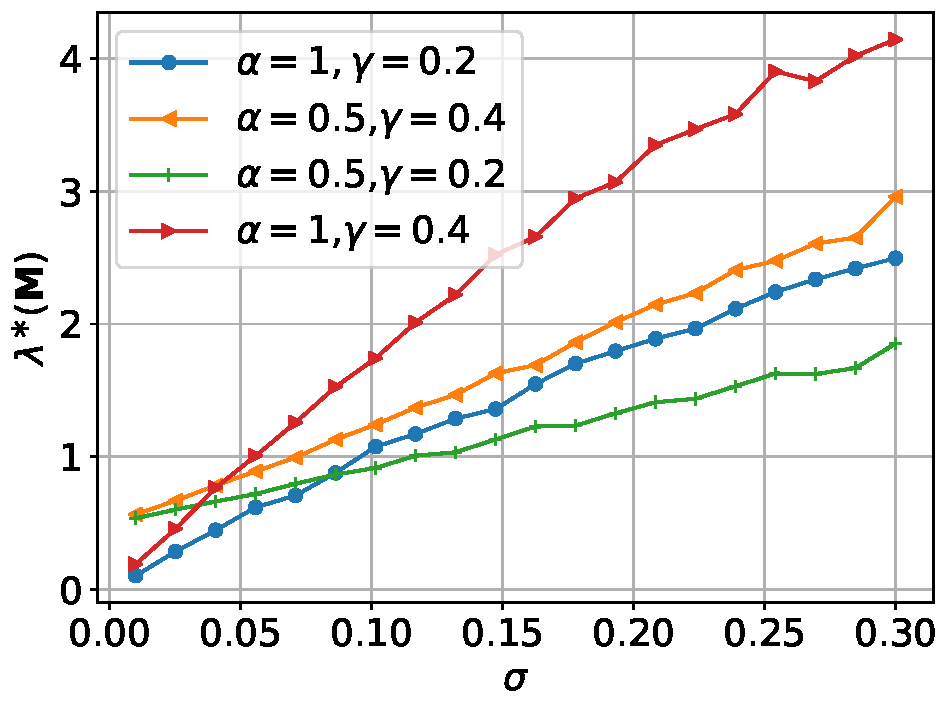
\includegraphics[width=0.6\columnwidth]{figures/converge/contraction_vs_variance_r1-crop.pdf}
  \caption{The largest singular value of $\bm{M}$ defined in \eqref{eq:matrix_m} versus variance of potential parameter $\bm{\theta}$. A value of each curve is the mean of $100$ graph realizations.}
  \label{fig:largest_singular}
\end{figure*}


In this section simulations on random graphs are carried out
to gain some insights on the $\alpha$-BP. The random graphs used here are generated
by the Erdos-R\'enyi (ER) model \cite{erdos1960}. In generating a graph by ER model, an edge between any two nodes is generated with probability $\gamma$, $\gamma \in (0,1)$.

Note that the MRF joint probability in \eqref{eq:mrf} can be reformulated into
\begin{equation}\label{eq:mrf_matrix_form}
  p(\bm{x}) \propto \exp\{-\bm{x}^{T}\bm{J}\bm{x} - \bm{b}^{T}\bm{x}\}, \bm{x} \in \bm{\Xx},
\end{equation}
with $\phi_{ts}(x_t, x_s) = e^{- 2 J_{t,s} x_t x_s}$ and $\phi_s(x_s) = e^{ - J_{s,s} x_s^2 - b_s  x_s}$. $\bm{J}$ here is the weighted adjacency matrix. In our experiments, we generate a random graph $\Gg = (\Vv, \Ee)$ with $\gamma$ by ER model and then associate potential factors to the graph. Specifically, factor $\phi_s(x_s)$ is associated to node $x_s$, $s \in \Vv$, and $\phi_{ts}$ to edge $(t, s) \in \Ee$. $J_{ts}$ is zero if these is no edge $(t, s)$.

For this set of experiments, we set $\Xx = \left\{ -1, 1 \right\}$ and $N=16$. To specify \eqref{eq:mrf_matrix_form}, the non-zero entries of $\bm{J}$ are sampled from a Gaussian distribution $\mathsf{N}(0, \sigma^2)$, i.e. $J_{ts} \sim \mathsf{N}(0, \sigma^2)$ if $J_{ts}\neq 0$. For entries of $\bm{b}$, we use $b_t \in \mathsf{N}(0, (\sigma/4)^2)$.
For each edge $(t,s) \in \Ee$, we set $\alpha_{ts}=\alpha$, i.e. the edges share a global value $\alpha$.

Figure~\ref{fig:largest_singular} illustrate how the largest singular value of $\bm{M}(\bm{\alpha}, \bm{\theta})$ as defined in \eqref{eq:matrix_m} changes when the standard deviation $\sigma$ of potential factors increases. The behavior is illustrated with different values of $\alpha$ and the edge probability $\gamma$. For each curve, a point on the curve is the mean of $100$ realizations of random graphs as described above. The curves of Figure~\ref{fig:largest_singular} show in general that a larger standard deviation of the potential factors of the graph edges makes it more difficult to fulfill the convergence condition in Theorem~\ref{thm:normd}. This is also the case when a graph is denser as we raise the edge probability $\gamma$ in generating random graphs, by comparing the green and orange curves. The comparison between green and blue curves indicates that the choice of $\alpha$ value in $\alpha$-BP also makes a difference, and its effect depends on the graph itself. Additionally, $\alpha$-BP with assignment $\alpha=0.5$ leads to flatter curves compared to standard BP ($\alpha=1$) and guarantees convergence for a larger range of $\sigma$, which corresponding a larger range of graphs.
How to tune $\alpha$ value to fulfill the condition of Theorem~\ref{thm:normd} depends not only on how dense ($\gamma$) the graph is, but also how potential factors spread out from each other.

\begin{figure*}[!t]
  \begin{subfigure}{0.5\textwidth}
    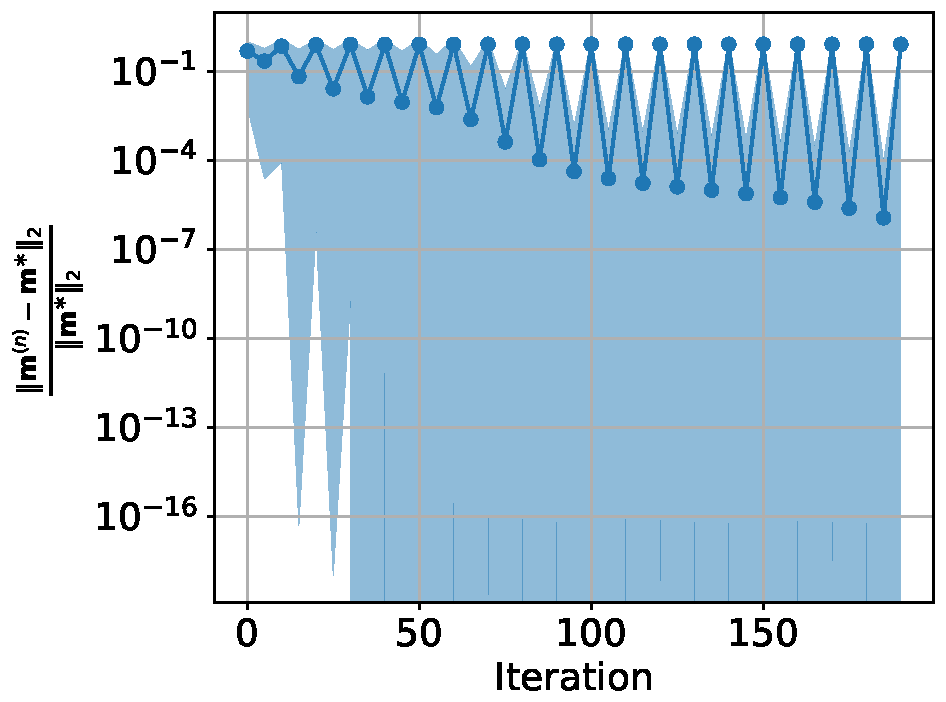
\includegraphics[width=1\columnwidth]
    {figures/converge/converge_erp0_4_alpha_1_stn_0_5_vs_filter_false_crop.pdf}
    \caption{}
    \label{fig:log-error-iter-diverse}
  \end{subfigure}
               %                the third figure
  \begin{subfigure}{0.5\textwidth}
    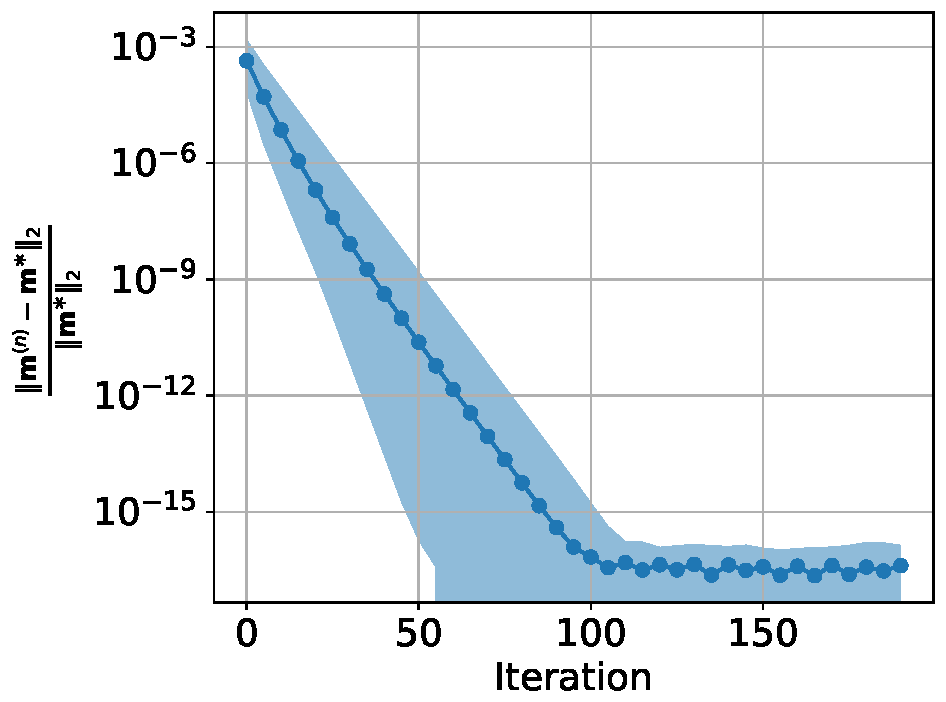
\includegraphics[width=1\columnwidth]{figures/converge/converge_erp0_2_alpha_0_5_stn_0_1_vs_filter_true-crop.pdf}
    \caption{}
    \label{fig:log-error-iter-converge}
  \end{subfigure}
  \caption{Numerical illustration of convergence, with normalized error ${\normd{\bm{m}^{(n)}-\bm{m}^{\ast}}}/{\normd{\bm{m}^{\ast}}}$ versus the number of iterations. Number of nodes $N=16$. (a) Parameter setting: $\gamma =0.4$, $\alpha = 1$ (equivalent to standard BP), $\sigma = 0.5$. (b) Parameter setting: $\gamma =0.2$, $\alpha = 0.5$, $\sigma = 0.1$.
    Blue region denotes the range from minimum to maximum of the normalized error of $100$ graph realizations, whereas the curve stands for mean error of the $100$ realized graphs. }
  \label{fig:convergence}
\end{figure*}



To illustrate our developed convergence condition for $\alpha$-BP, we also observe how messages in a graph changes along belief propagation iterations. To be specific, we run our $\alpha$-BP with $200$ iterations on a graph, after which the messages in the graph are denoted by $\bm{m}^{\ast}$. $\bm{m}^{\ast}$ can be the converged messages if $\alpha$-BP has converged within the $200$ iterations. Then we measure the quantity $\normd{\bm{m}^{(n)} - \bm{m}^{\ast}}/\normd{\bm{m}^{\ast}}$ during the iterations. In Figure~\ref{fig:log-error-iter-diverse}, we generate $100$ random graphs by ER model with parameter setting as $\gamma =0.4$, $\alpha = 1$\footnote{$\alpha=1$ in $\alpha$-BP corresponding to standard BP.}, $\sigma = 0.5$. By referring to the curves in Figure~\ref{fig:largest_singular}, it can be seen that this setting does not fulfill the condition in Theorem~\ref{thm:normd}. The log error changes versus iteration number $n$ for the $100$ graphs are shown in Figure~\ref{fig:log-error-iter-diverse}, in which the blue region indicates the range and the solid curve indicates the mean of the normalized errors. It is clear that Figure~\ref{fig:log-error-iter-diverse} does not show any sign of convergence within $200$ iterations.

\begin{figure*}[!t]
               %                the first figure
  \begin{subfigure}{0.5\textwidth}
    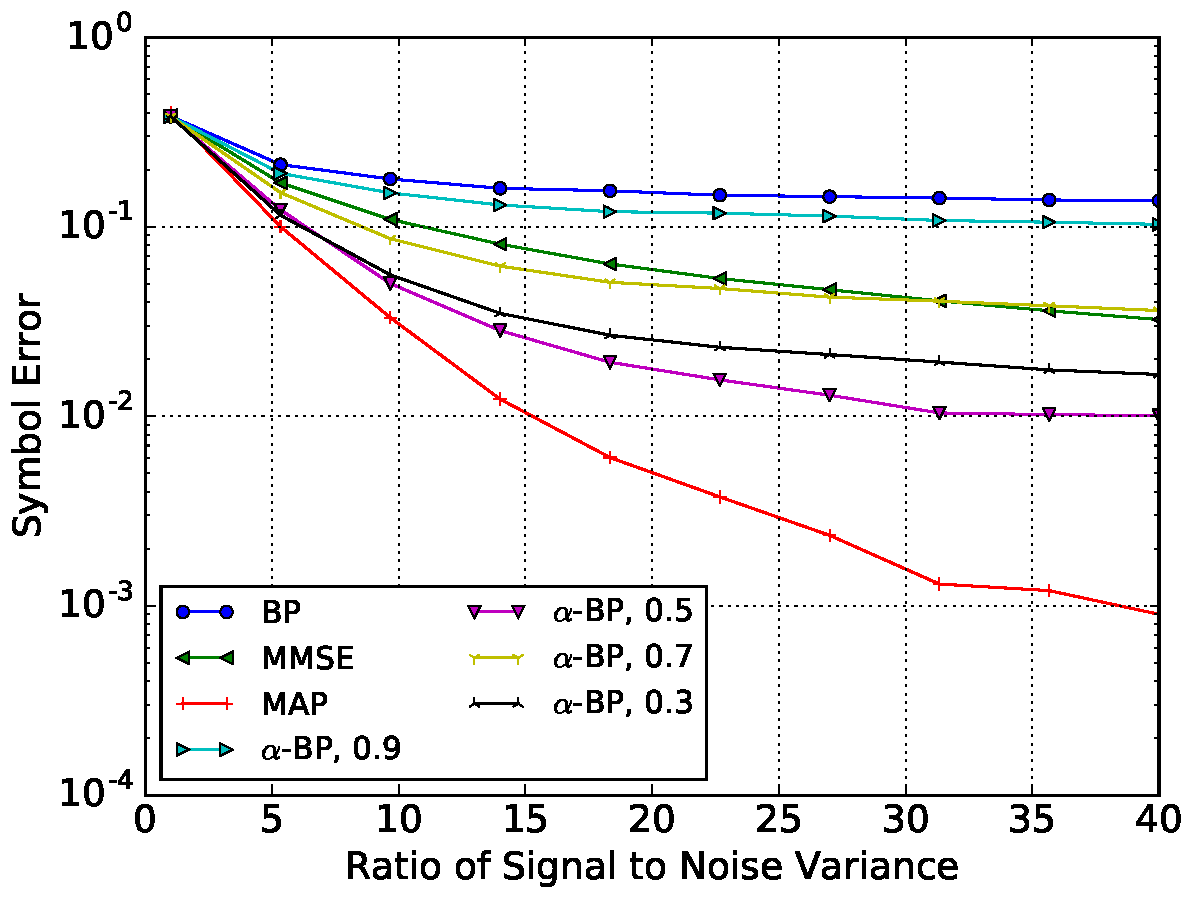
\includegraphics[width=1\columnwidth]{figures/alpha_compare_crop.pdf}
    \caption{}
    \label{fig:mimo_a}
  \end{subfigure}
  \begin{subfigure}{0.5\textwidth}
    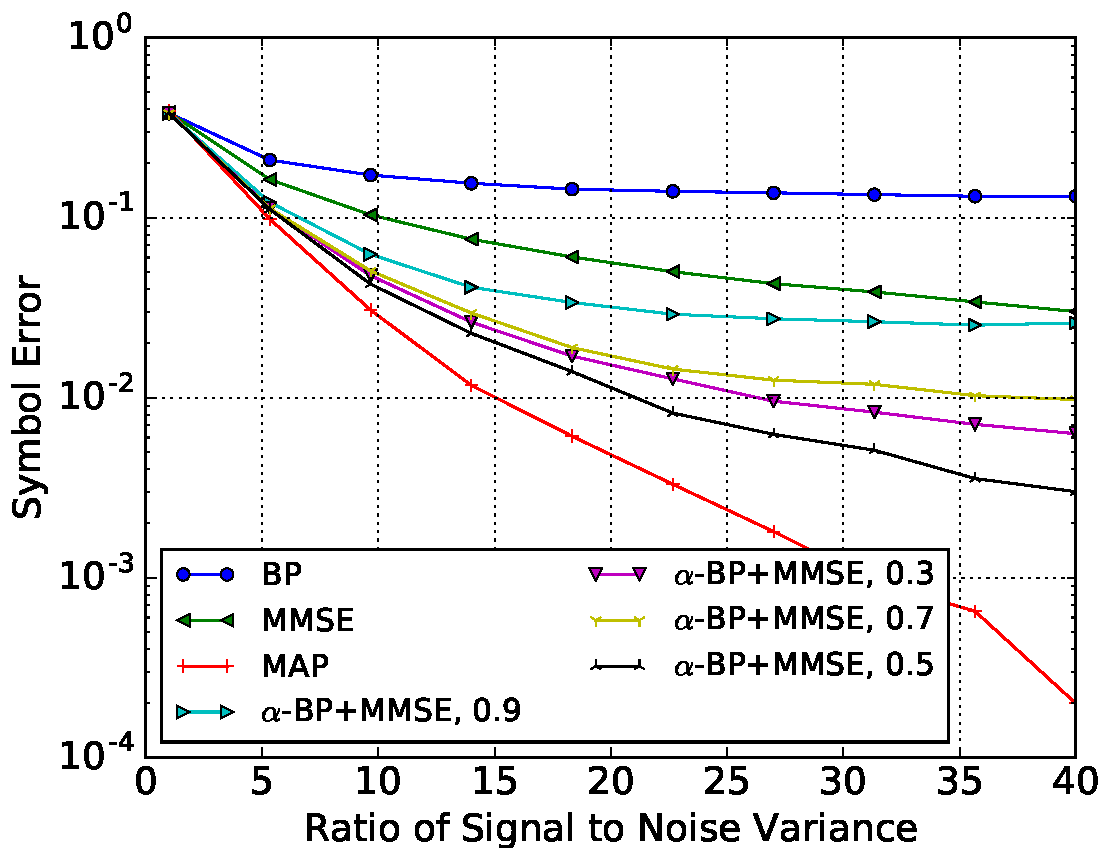
\includegraphics[width=1\columnwidth]{figures/prior_mmse_alpha_compare_crop.pdf}
    \caption{}
    \label{fig:mimo_b}
  \end{subfigure}
  \begin{subfigure}{0.5\textwidth}
    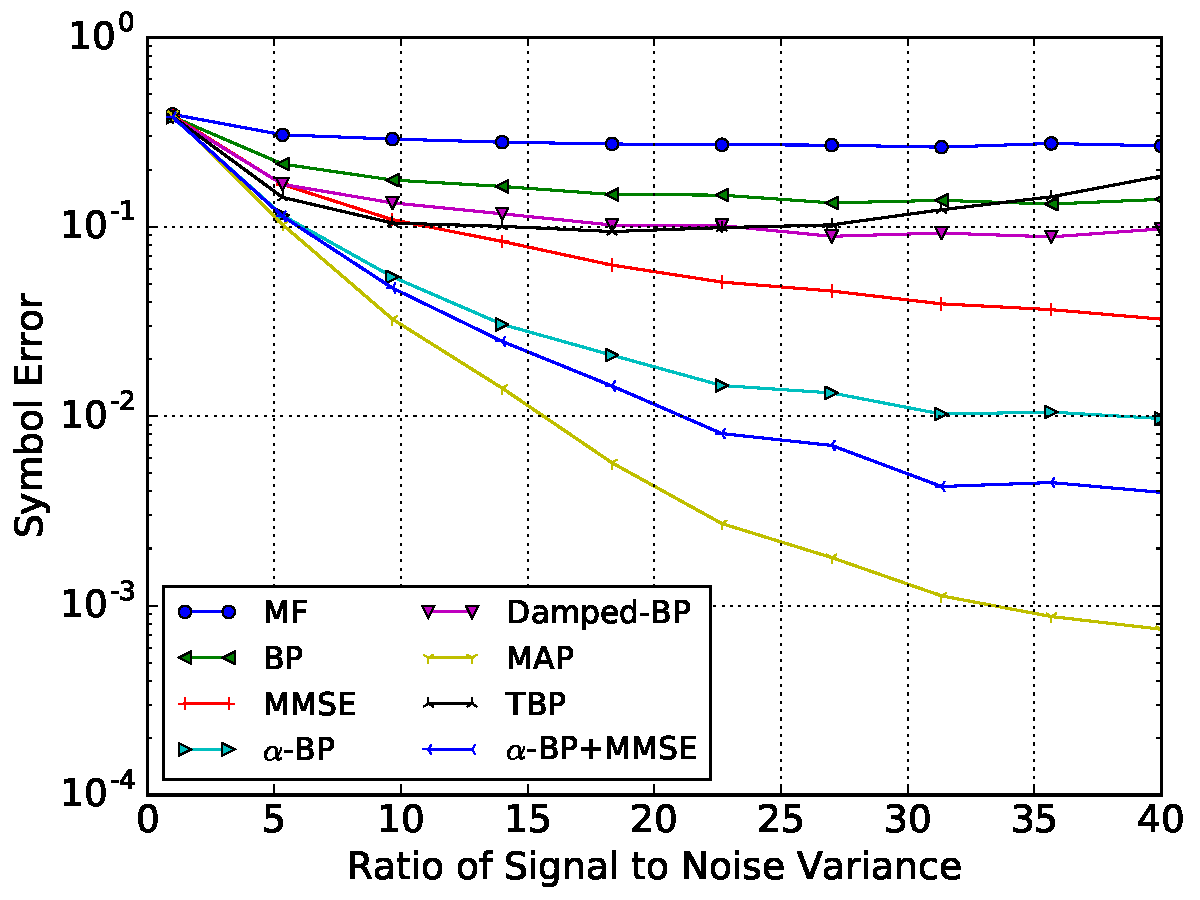
\includegraphics[width=1\columnwidth]{figures/tbp/mf_tbp_compare.pdf}
    \caption{}
    \label{fig:mimo_c}
  \end{subfigure}
  \caption{Numerical results of $\alpha$-BP: symbol error of MIMO detection.}
  \label{fig:mimo_detection}
\end{figure*}

We then carry out a set of experiments in Figure~\ref{fig:log-error-iter-converge} similar to our experiments in Figure~\ref{fig:log-error-iter-diverse}. The only difference lies in the graph generating process. Here we set the parameters to be $\gamma =0.2$, $\alpha = 0.5$, $\sigma = 0.1$. According to our curves in Figure~\ref{fig:largest_singular}, a graph generated with this parameter setting should fulfill the condition in Theorem~\ref{thm:normd}. Due to randomness of both graph generating by ER and potential factors, we regenerate a graph if the initial generated graph does not satisfy $\lambda^{\ast}(\bm{M})<1$. Therefore the $100$ graphs used in experiments for Figure~\ref{fig:log-error-iter-converge} all fulfill the Theorem~\ref{thm:normd}. The result in Figure~\ref{fig:log-error-iter-converge} is consistent with our analysis on the convergence of $\alpha$-BP.



\subsection{Complete Graph Case: Application to MIMO Detection}

In this section, we show the application of $\alpha$-BP to a multiple input multiple output (MIMO) detection problem. For a MIMO system, the observation $\bm{y}$ is a linear function of the channel $\bm{H}\in \RR^{N\times N}$ when the unknown signal $\bm{x}$ needs to be detected,
\begin{equation}\label{eq:linear-model}
  \bm{y} = \bm{H} \bm{x} + \bm{e}, \bm{x} \in \bm{\Xx},
\end{equation}
where $\bm{e}$ is  noise modeled as Gaussian noise $ \bm{e} \sim \mathsf{N}\left( \bm{0}, \sigma^2_{w} \bm{I} \right)$. Here $\bm{I}$ is \textit{unitary} matrix. In this case, the posterior of $\bm{x}$ can be written as:
\begin{align}\label{eq:true-posterior}
  p(\bm{x}|\bm{y}) &\propto e^{ - \frac{1}{2\sigma_w^2} \normd{\bm{Hx} - \bm{y}}^2 } \nonumber \\
                   & = e^{ - \frac{1}{2\sigma_w^2}\left[ \bm{x}^{T}\bm{H}^{T}\bm{H}\bm{x} - 2 \bm{y}^T\bm{H}\bm{x}  + \bm{y^T}\bm{y}  \right] }.
\end{align}
Denote $\bm{S} = \bm{H}^T\bm{H}$, $\bm{h}_i$ as the $i$-th column of $\bm{H}$, and
\begin{align}
  \phi_{i}(x_i) =& e^{- \frac{S_{i,i} x_i^2}{2 \sigma_w^2} + \frac{\langle {\bm{h}_i, \bm{y}}\rangle x_i}{\sigma_w^2} },\nonumber \\
  \phi_{ij}(x_i, x_j) =& e^{ -\frac{x_i S_{i,j} x_j}{\sigma_w^2} }.
\end{align}
Then it can be seen that \eqref{eq:true-posterior} is an instance of \eqref{eq:mrf}. We set $\Xx = \left\{ -1, 1 \right\}$, $N = 8$, and let $\bm{H}\in \RR^{8 \times 8}$ be sampled from a Gaussian distribution.

We test the application of $\alpha$-BP to the MIMO signal detection numerically. We run the $\alpha$-BP, without the prior trick (Section~\ref{subsec:remark}) in Figure~\ref{fig:mimo_a} and with the prior in Figure~\ref{fig:mimo_b} (legend ``$\alpha$-BP$+$MMSE'') as estimation of minimum mean square error (MMSE). The reference results of MMSE and maximum a posterior (MAP, exhausted search) are also reported under the same conditions. MMSE estimator depends on Gaussian posterior $\mathsf{N}(\hat{\bm{\mu}}, \hat{\bm{\Sigma}})$, where $\hat{\bm{\mu}} = (\bm{H}^{T}\bm{H} + \sigma_w^2 \bm{I})^{-1}\bm{H}^{T}\bm{y}$ and $\hat{\bm{\Sigma}} = (\bm{H}^{T}\bm{H} + \sigma_w^2 \bm{I})^{-1}\sigma_w$. Detection of MMSE carried out by $\argmin_{x_i\in \Xx}\abs{x_i-\hat{\mu}_i}$.% The prior belief used in ``$\alpha$-BP$+$MMSE'' is $\hat{p}(x_i)=\Nn(\hat{{\mu}}_i, \hat{\bm{\Sigma}}_{i,i})$.

Figure~\ref{fig:mimo_a} shows that BP even underperforms MMSE but $\alpha$-BP can outperform MMSE by assigning smaller value of $\alpha$.
Note that MMSE has a higher computation complexity since it requires the matrix inverse computation whose complexity is proportional to $N^3$. Therefore $\alpha$-BP is superior to MMSE both performance-wise and complexity-wise.  
                         %                          $\alpha$-BP does not have this problem and still can outperform MMSE. 
However, there is still a big gap between $\alpha$-BP (even for $\alpha=0.5$) and MAP. This gap can be decreased further by using the prior trick discussed in Section~\ref{subsec:remark}. Figure~\ref{fig:mimo_b} exemplifies this effects by using prior belief from MMSE, $\hat{p}_i(x_i)\propto \exp\{-(x_i-\hat{\mu}_i)^2/(2\hat{\bm{\Sigma}}_{i,i})\}$, by modifying the graph as shown in Figure~\ref{fig:factor-graph-with-prior}, which comes with legend "$\alpha$-BP$+$MMSE". It is shown that larger performance gain is observed when $\alpha$-BP runs with prior belief.

Additional, we also carry out the experiments where the proposed $\alpha$-BP is compared with mean field (legend 'MF'), BP with damping technique \cite{Pretti2005damping} (with legend 'Damped-BP'), and Tree-reweighted belief propagation \cite{wainwright2008graphical} (with legend 'TBP') in Figure~\ref{fig:mimo_c}. As expected, mean field method performs no better than BP. Damping technique improves BP's performance with a noticeable difference but still falls behind MMSE. The performance of tree-reweighted BP reaches that of MMSE in low ratio range of signal-to-noise variance but degenerates a lot in the high ratio range. The old message and potential factors are reweighted by the edge appearance probability in TBP to compute new messages. In TBP, the edge appearance probability is the probability that the edge exists in a randomly chosen spanning tree from all possible spanning trees of graph $\Gg$, which is usually expensive to compute.

\section{Summary}

In this chapter, we studied belief propagation in the way of $\alpha$-divergence minimization and proposed an alternative belief propagation method. The alternative method was connected and compared with the classic approximate iterative inference methods, namely mean filed, loopy belief propagation and tree-reweighted belief propagation. The connection and comparison were made with regard to both the high-level optimization objectives and the practical iterative update rules. All methods share a common interpretation, \textit{inference an optimization}, i.e., inference methods could be recovered from  optimization problems (free energy minimization or a divergence minimization). Although they started from different optimization cost functions, the derived iterative update rules share some similarities. The study enriches our insight into deterministic approximate inference approaches.

Given the wide application of the family of belief propagation methods, when the implementation of them can have guaranteed convergence is a fundamental question, which is of practical interest in general. This issue was addressed in the binary support case in this chapter via the method of contraction condition. The derived sufficient conditions for $\alpha$-BP gives us sufficient conditions about whether we can expect it to converge. The sufficient conditions allow us to check if $\alpha$-BP is guaranteed to converge without actually running the algorithm for a given problem.

Another essential question is about the error of deterministic approximate inference, compared with the exact answer. This problem is surely challenging. There is little work offering error-bounded methods in deterministic approximate inference family. Due to the lack of knowledge here, manual turning or trial-and-error is still not able to be avoided in practical system implementations. The development towards automated inference methods with at least less manual work is always an important direction in this track. 

\section{Relevant Literature}
\label{chpt3:sec:literature}
Approximate inference is applicable to wide range of settings. The wide applications include but are not limited to imaging processing \cite{zhang2013denoise}, multi-input-multi-output (MIMO) signal detection in digital communication \cite{cespedes2014ep,jeon2015optimality}, inference on structured lattice \cite{10.2307/25651244}, and machine learning \cite{2018arXiv180607066M, Lin:2015:DLM:2969239.2969280, yoon2019inferenceGraph}. The empirical success of  belief propagation (BP) rules came much earlier than its theoretical examination, which dates back to $80$s in last century\cite{pearl1986b}.

As a result of the representation power of probabilistic graphical models, graphs with loops are inevitable in real-world problems. Before there was any justification, problems represented by graphs with loops simply employ BP as if there was no loop, i.e. loopy BP.  Although loopy BP is still a practical method to do inference approximately, its performance varies from case to case and its behavior is not well understood in general. A direct workaround is to propagate messages on a manipulated graph instead of the original graph. The representative methods of this family are junction tree (clique tree) method \cite[Section~10]{koller2009pgm} and generalized belief propagation (GBP)\cite{yedida2005constucting}. Although they both cluster multiple nodes of the original graph into a node in a hyper-graph (clique tree or region graph) and propagate message in the new graph. Junction tree method provides an exact inference method while GBP is an approximate inference method. How to convert a general graph to a junction tree or region graph is not trivial, and the structure of the converted graph makes a significant difference in the inference performance. Additionally, the former's complexity relies on tree-width (the size of the largest clique minuses one), which means that there is not too much to gain by using junction tree compared to enumerating configurations in very dense graphs. For the latter, constructing a region graph itself is a challenging task and still needs further study.


Apart from the work of transforming the problem represented by a loopy graph into one of a hyper-graph, research is more active in approximate methods. Starting from the stationary point explanation of Bethe free energy in \cite{Yedidia:2000:GBP:3008751.3008848}, variants of BP have been derived to improve BP in a general graph. Fractional BP in \cite{Wiegerinck:2002:FBP:2968618.2968673} applies a correction coefficient to each factor and obtain a message passing rule similarly as minimization of Bethe free energy. 
Generalized BP in \cite{Yedidia:2000:GBP:3008751.3008848} propagates belief between different regions of a graph, and damping BP in \cite{Pretti2005damping} updates beliefs by combining old and new beliefs. \cite{wainwright2008graphical} relaxes a Bethe free energy into an upper bound of the partition function and the tree-reweighed BP is obtained. Technique such as damping is also explored to seek convergence of BP and its variants \cite{Pretti2005damping}.
Another track falls to the variational method framework, introduced by Opper and Winther \cite{Opper:2000:GPC:1121900.1121911} and Minka \cite{Minka:2001:EPA:647235.720257, Minka:2001:FAA:935427}, namely expectation propagation (EP). In EP, a simpler factorized distribution defined in exponential distribution family is used to approximate the original complex distribution, and an intuitive factor-wise refinement procedure is used to find such an approximate distribution. The method intuitively minimizes a localized Kullback-Leibler (KL) divergence. This is discussed further in \cite{divergence-measures-and-message-passing} and shows a unifying view of message passing algorithms. The following work, stochastic EP by \cite{yingzhen2015sep}, explores EP's variant method for applications to large datasets.

Due to the fundamental role of BP for probabilistic inference and related applications, research of seeking insight into BP performance and study on its convergence have been constantly carried out. \cite{weiss2000correctness} presents the convergence condition of BP in graphs containing a single loop. Work in \cite{heskes2004uniqueness} analyzes the Bethe free energy and offers sufficient conditions on the uniqueness of BP fixed point.
{Closely related to the content of this chapter, \cite{mooij2012sufficient-conditions} studies the sufficient conditions for BP convergence to a unique fixed point ($\alpha$-BP generalizes BP).}
\cite{nima2013stochasticBP} proposes a stochastic BP algorithm for high-dimensional discrete spaces and gives the convergence conditions of it. \cite{frederic2019fast} shows that BP can converge to global optima of Bethe energy when BP runs in Ising models that are ferromagnetic (neighboring nodes prefer to be aligned).
There are also works trying to give insight on variant methods of BP. Namely,
\cite{du2017convergenceBP, malioutov2006walk-sums} studies the convergence condition of Gaussian BP inference over distributed linear Gaussian models. \cite{roosta2008reweighed_sum_product} gives the convergence analysis of a reweighted BP algorithm, and offers the necessary and sufficient condition for subclasses of homogeneous graphical models with identical potentials.



%%% Local Variables:
%%% mode: latex
%%% TeX-master: "../../main"
%%% End:



% chapter 4
\chapter{Inference as Optimization: An Region-based Energy Method}
\label{chapter4}
In the previous chapter, we presented an iterative message passing algorithm and discussed the connection with mean field, belief propagation, and tree-reweighted belief propagation algorithms. These methods fellow different message passing rules (fixed-point iterations) that have been heuristically developed.
The heuristic efforts usually include the message-passing rules, message update schedules, manual tuning and trials for convergence to stable solutions. Sometimes, it needs to switch to an alternative approximate inference method if the initial selection can not meet practical requirements, e.g., belief propagation can be exact in tree-structured graphs but generally performs worse than mean field method in densely-connected graphs.
However, on our way towards automated inference methods, we intend to reduce the heuristic efforts and manual trials without degenerating their performance. In this chapter, we discuss one promising way to achieve this target. The principle idea is to do inference by solving an optimization problem, i.e., to treat inference as optimization.

In fact, we have touched this topic in Section~\ref{chpt2:sec:variational-inference}, where we interpreted what message passing updates of mean field and belief propagation are actually doing. It turns out that the message passing rules are fixed-point iterations as solutions to optimization problems. Therefore mean field and belief propagation get the intuition of minimization of variational free energy. Take the most widely used belief propagation method as an example, since the message passing rule can be obtained from the minimization of Bethe free energy cost, we may just as well solve the optimization problem by other optimization techniques such as gradient descent. However, an early attempt on this track showed that it might suffer from stability issues for peaky potential functions compared to iterative message passing method \cite{welling2001belief}.


Another limitation lies in the Bethe approximation itself. When representing the Bethe approximation in a factor graph, a factor node associated with a potential function is related to more than one random variable, while a variable node is associated with one random variable. When beliefs are propagated on the graph, only a univariate marginal distribution (associated with a variable node) can be propagated from one neighboring factor to another neighboring factor of the variable node. The interactions between multiple variables cannot be directly propagated as messages in the graph. This limitation actually affects the performance of Bethe approximation in general graphs, especially the loopy graphs.

In this chapter, we seek to use larger clusters in a graphical representation to overcome the above-mentioned limitation. Along with that, we would bring the concept of inference as optimization into the representation with clusters.




\begin{figure}[!t]
  \centering
  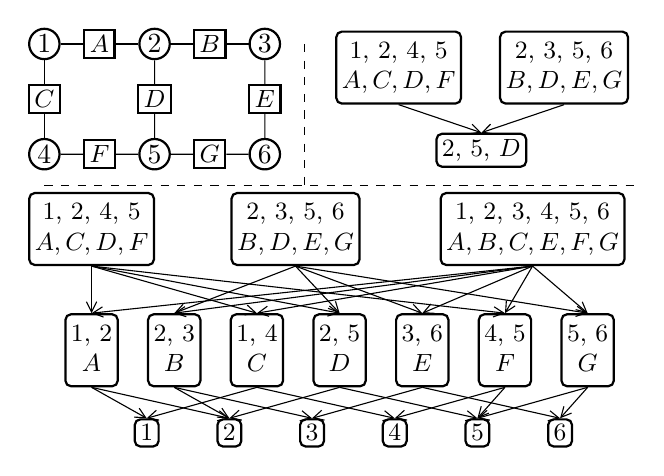
\begin{tikzpicture}
    \begin{scope}[scale=0.7]

      \tikzstyle{cnode} = [thick, draw=black, circle, inner sep = 1pt,  align=center]
      \tikzstyle{nnode} = [thick, rectangle, rounded corners = 0pt,draw,inner sep = 2pt]
      \node[cnode] (x1) at (0,0) {1};
      \node[cnode] (x2) at (2,0) {2};
      \node[cnode] (x3) at (4,0) {3};

      \node[cnode] (x4) at (0,-2) {4};
      \node[cnode] (x5) at (2,-2) {5};
      \node[cnode] (x6) at (4,-2) {6};

      \node[nnode] (fa) at (1,0) {\small$A$};
      \node[nnode] (fb) at (3,0) {\small$B$};

      \node[nnode] (fc) at (0,-1) {\small$C$};
      \node[nnode] (fd) at (2,-1) {\small$D$};
      \node[nnode] (fe) at (4,-1) {\small$E$};
      
      \node[nnode] (ff) at (1,-2) {\small$F$};
      \node[nnode] (fg) at (3,-2) {\small$G$};


      \draw[-] (x1) -- (fa);
      \draw[-] (x1) -- (fc);

      \draw[-] (x2) -- (fa);
      \draw[-] (x2) -- (fb);
      \draw[-] (x2) -- (fd);

      \draw[-] (x3) -- (fb);
      \draw[-] (x3) -- (fe);

      \draw[-] (x4) -- (fc);
      \draw[-] (x4) -- (ff);

      \draw[-] (x5) -- (fd);
      \draw[-] (x5) -- (ff);
      \draw[-] (x5) -- (fg);

      \draw[-] (x6) -- (fe);
      \draw[-] (x6) -- (fg);

    \end{scope}
    \draw[dashed] (0, -1.8) -- (7.5, -1.8) (3.3, 0) -- (3.3, -1.8);
    
    \begin{scope}[xshift=4.5cm, yshift=-0.3cm,scale=0.7]
      \tikzstyle{rnode} = [thick, rectangle, rounded corners = 2pt,minimum size = 0.0cm,draw,inner sep = 2pt]
      \node[rnode] (r01) at (0,0) {\small \begin{tabular}[x]{@{}c@{}}1, 2, 4, 5 \\ $A,C,D,F$ \end{tabular}};
      \node[rnode] (r02) at (3,0) {\small \begin{tabular}[x]{@{}c@{}}2, 3, 5, 6\\ $B,D,E,G$ \end{tabular}};
      \node[rnode] (r11) at (1.5, -1.5) {\small 2, 5, $D$};

      \draw[->] (r01.south) -- (r11.north);
      \draw[->] (r02.south) -- (r11.north);

    \end{scope}

    \begin{scope}[xshift=0.6cm, yshift=-2.35cm,scale=0.7]
      \tikzstyle{rnode} = [thick, rectangle, rounded corners = 2pt,minimum size = 0.0cm,draw,inner sep = 2pt]
      \node[rnode] (r01) at (0,0) {\small\begin{tabular}[x]{@{}c@{}}1, 2, 4, 5 \\ $A,C,D,F$ \end{tabular}};
      \node[rnode] (r02) at (3.7,0) {\small\begin{tabular}[x]{@{}c@{}}2, 3, 5, 6\\ $B,D,E,G$ \end{tabular}};
      \node[rnode] (r03) at (8,0) {\small\begin{tabular}[x]{@{}c@{}}1, 2, 3, 4, 5, 6\\ $A,B,C,E,F,G$ \end{tabular}};
      \begin{scope}[yshift=-0.2cm]
        \node[rnode] (r11) at (0, -2.0) {\small\begin{tabular}[x]{@{}c@{}}1, 2\\ $A$ \end{tabular}};
        \node[rnode] (r12) at (1.5, -2.0) {\small\begin{tabular}[x]{@{}c@{}}2, 3\\ $B$ \end{tabular}};
        \node[rnode] (r13) at (3, -2.0) {\small\begin{tabular}[x]{@{}c@{}}1, 4\\ $C$ \end{tabular}};
        \node[rnode] (r14) at (4.5, -2.0) {\small\begin{tabular}[x]{@{}c@{}}2, 5\\ $D$ \end{tabular}};
        \node[rnode] (r15) at (6, -2.0) {\small\begin{tabular}[x]{@{}c@{}}3, 6\\ $E$ \end{tabular}};
        \node[rnode] (r16) at (7.5, -2.0) {\small\begin{tabular}[x]{@{}c@{}}4, 5\\ $F$ \end{tabular}};
        \node[rnode] (r17) at (9, -2.0) {\small\begin{tabular}[x]{@{}c@{}}5, 6\\ $G$ \end{tabular}};

        \begin{scope}[yshift=0.5cm]
          \node[rnode] (r21) at (1, -4) {\small 1};
          \node[rnode] (r22) at (2.5, -4) {\small 2};
          \node[rnode] (r23) at (4, -4) {\small 3};
          \node[rnode] (r24) at (5.5, -4) {\small 4};
          \node[rnode] (r25) at (7, -4) {\small 5};
          \node[rnode] (r26) at (8.5, -4) {\small 6};
        \end{scope}
      \end{scope}
      % edge level0 to level1
      \draw[->] (r01.south) -- (r11.north);
      \draw[->] (r03.south) -- (r11.north);

      \draw[->] (r02.south) -- (r12.north);
      \draw[->] (r03.south) -- (r12.north);

      \draw[->] (r01.south) -- (r13.north);
      \draw[->] (r03.south) -- (r13.north);

      \draw[->] (r01.south) -- (r14.north);
      \draw[->] (r02.south) -- (r14.north);

      \draw[->] (r02.south) -- (r15.north);
      \draw[->] (r03.south) -- (r15.north);

      \draw[->] (r01.south) -- (r16.north);
      \draw[->] (r03.south) -- (r16.north);

      \draw[->] (r02.south) -- (r17.north);
      \draw[->] (r03.south) -- (r17.north);

      % edge level1 to level2
      \draw[->] (r11.south) -- (r21.north);
      \draw[->] (r13.south) -- (r21.north);

      \draw[->] (r11.south) -- (r22.north);
      \draw[->] (r12.south) -- (r22.north);
      \draw[->] (r14.south) -- (r22.north);


      \draw[->] (r12.south) -- (r23.north);
      \draw[->] (r15.south) -- (r23.north);

      \draw[->] (r13.south) -- (r24.north);
      \draw[->] (r16.south) -- (r24.north);

      \draw[->] (r14.south) -- (r25.north);
      \draw[->] (r16.south) -- (r25.north);
      \draw[->] (r17.south) -- (r25.north);

      \draw[->] (r15.south) -- (r26.north);
      \draw[->] (r17.south) -- (r26.north);
    \end{scope}
  \end{tikzpicture}
  \caption{Illustration of a factor graph for 2-by-3 grid (top left, variable nodes are indexed by number and factor nodes by letters), and two alternative regions graphs (two levels for the top right one and three levels for bottom one) constructed from the factor graph.}
  \label{fig:factor-region-graphs}
\end{figure}

\section{Region Graph and Generalized Belief Propagation}

In a MRF, the underlining probability distribution of its $N$-dimensional random vector $\bm{x}=(x_1, x_2, \cdots, x_N)$ can be written as
\begin{equation}\label{eq:joint-px}
  p(\bm{x}; \bm{\theta}) = \frac{1}{Z(\bm{\theta})} \prod_{a \in \Ff} \phi_{a}(\bm{x}_{a}; \bm{\theta}_a),
\end{equation}
where potential functions' index set is instantiated as $\Ff = \left\{ A, B, \cdots, M \right\}$. Here we explicitly define that potential $\phi_a$ has its own parameter $\bm{\theta}_a$, and $\bm{\theta} = \{\bm{\theta}_a, a\in \Ff\}$. For notation simplicity, we define that each variable has $K$ states, i.e. $x_i \in \Xx_i$ with $|\Xx_i|=K$, where $|\cdot|$ denotes the cardinality.

We have discussed that loopy BP as a message-passing algorithm operates on factor graphs (as shown in the top-left example in Figure~\ref{fig:factor-region-graphs}) in Section~\ref{chpt2:sec:variational-inference}. We then can compute the marginal distributions of \eqref{eq:joint-px} from a collection of updated messages as discussed in Chapter~\ref{chapter3}. The fundamental limitation of methods in this family is that a message over a single variable is communicated instead of messages over multiple variables (as pointed out above). This issue can be relieved by using a hyper-graph or cluster graph where a node is associated with multiple variables. A region graph is such a kind of graph, which was proposed by \cite{yedida2005constucting, DBLP:journals/corr/abs-1207-4158} to assist scheduling messages for generalized belief propagation (GBP). For illustration purpose, two alternative region graphs constructed from the same factor graph are shown in Figure~\ref{fig:factor-region-graphs}.

Before giving the definition of a region graph, we need to define the \textit{region} first, which is on the basis of a factor graph $\Gg_{\Ff}(\Vv \cup \Ff, \Ee_{\Ff})$ (see Definition~\ref{chpt2:def:factor-graph}).
\begin{definition}
  A \textit{region} $R$ is a set $V_R$ of variables nodes and a set $A_R$ of factor nodes, such that if a factor node $a$ belong to $A_R$, all the variables nodes neighboring $a$ are in $V_R$.
\end{definition}
A region in a region graph acts as a node, and there are directed edges between regions which are defined according to specific rules. Formally, a region graph is defined as follows:
\begin{definition}\label{def:region-graph}
  A \textit{region graph} is  a directed graph $\Gg_R(\Rr, \Ee)$, where each vertex $R \in \Rr$ is defined as the joint set of variable and factor nodes in this region, i.e. $R = \left\{ i \in V_R, a \in A_R | i \in \Vv, a \in \Ff \right\}$. Each edge $e \in \Ee$ in $\Gg_R$ is directed from $R_p$ to $R_c$ such that $R_c \subset R_p$. 
\end{definition}


We define some notations before going further. Since $\Gg_R$ is a hierarchical directed graph, $\Rr_l$ denotes the set of regions at level $l$, and
$R^{[l]}_i\in \Rr_l$ is the $i$-th region node at level $l$. This means $\Rr_0$ is a set of the top root regions that have no parents, i.e. the level $0$ regions. Also, $R^{[l]}$ means it can be any node in $\Rr_l$ and $R$ denotes a region node when it is not clear or does not matter at which level it locates. Lastly, since a region may be associated with both variable and factor nodes, we denote the scope of $R$ by  $\bm{x}_R = \left\{ x_i| i \in R \right\}$.

\begin{example}
  Take the top-right region graph in Figure~\ref{fig:factor-region-graphs} as an example. There are total two layers in the region graph, i.e., $\Rr_0$ and $\Rr_1$. We have $\Rr_0 = \left\{ R_1^{[0]}, R_2^{[0]} \right\}$ where $R_1^{[0]} = \left\{ 1, 2, 4, 5, A, C, D, F \right\}$ and $R_2^{[0]} = \left\{ 2, 3, 5, 6, B, D, E, G \right\}$. As for $\Rr_1$, there is only one region in it and it is $R_1^{[1]} = \left\{ 2, 5, D \right\}$. There are two directed edges, i.e., $\left( R_1^{[0]}, R_1^{[1]} \right)$ and $\left( R_2^{[0]}, R_1^{[1]} \right)$.
\end{example}

GBP operates on a region graph $\Gg_R(\Rr,\Ee)$. A message is always sent from a parent region $P$ to a child region $R$, i.e., along the directed edge $(P, R)\in \Ee$. Let us define the factors in region $R$ as $A_R = \left\{ a | a \in R \right\}$. $\Pp(R)$ denotes the set of parent regions of $R$. The descendants of $R$ is denoted by $\Dd(R)$ (excluding $R$). The descendants of $R$ including $R$ is denoted by $\hat{\Dd}(R) = \Dd(R) \cup R$. The message update rule from the parent region $P$ to the child region $R$ is
\begin{align}\label{chpt4:eq-gbp-update-rule}
  m_{P\rightarrow R} \propto \frac{\sum_{\bm{x}_P\backslash
  \bm{x}_R}\prod_{a\in A_P\backslash A_R}\phi_a(\bm{x}_a)\prod_{(I,J)
  \in \Nn(P, R)}m_{I\rightarrow J}(\bm{x}_J)}{\prod_{(I,J)
  \in \Hh(P, R)}m_{I\rightarrow J}(\bm{x}_J)},
\end{align}
where $\Nn(P, R)$ is the set of all connected pairs of regions $(I, J)$ such that $J$ is in $\hat{\Dd}(P)$ but not $\hat{\Dd}(R)$ while $I$ is not in $\hat{\Dd}(P)$, $\Hh(P, R)$ is the set of all connected pairs of regions $(I, J)$ such that $J$ is in $\hat{\Dd}(R)$ while $I$ is in $\hat{\Dd}(P)$ but not $\hat{\Dd}(R)$. They are formally defined as
\begin{align}\label{chpt4:eq:gbp-two-sets}
  \Nn(P, R) &:= \left\{ (I,J)\in \Ee | J \in \hat{\Dd}(P) \backslash \hat{\Dd}(R), I \not\in \hat{\Dd}(P)\right\},\nonumber \\
  \Hh(P, R) &:= \left\{ (I,J) \in \Ee | J \in \hat{\Dd}(R), I \in \hat{\Dd}(P) \backslash \hat{\Dd}(R), (I,J) \neq (P,R) \right\}.
\end{align}
By comparing the GBP with previously discussed mean field, loopy BP and $\alpha$-BP in Chapter~\ref{chapter2} and \ref{chapter3}, it can be seen that the message update of GBP is more complex. The ordering or sequence of GBP message updates in a region graph also affects its performance (e.g., see \cite{yedida2005constucting}). After the message passing phase, the belief for each region $R$, i.e., the approximation to marginal $p(\bm{x}_{R})$, is computed as
\begin{align}\label{chpt4:gbp-belief-rule}
  b_R(\bm{x}_R) \propto \prod_{a\in A_R} \phi_a(\bm{x}_a) \prod_{P\in
  \Pp(R)} m_{P\rightarrow R}(\bm{x}_R) \prod_{D\in \Dd(R)} \prod_{P^{\prime} \in \Pp(D) \backslash \hat{\Dd}(R)} m_{P^{\prime}\rightarrow D}(\bm{x}_D).
\end{align}


\begin{example}
  We demonstrate an example of GPB message update using the three-level region graph in Figure~\ref{fig:factor-region-graphs}. Following our notation, we have $\Rr_0 = \left\{ R_1^{[0]}, R_2^{[0]}, R_3^{[0]} \right\}$ where $R_1^{[0]} = \left\{ 1, 2, 4, 5, A, C, D, F \right\}$, $R_2^{[0]} = \left\{ 2, 3, 5, 6, B, D, E, G \right\}$, and $R_3^{[0]} = \left\{ 1, 2, 3, 4, 5, 6, A, B, C, D, F, G \right\}$. For $\Rr_1$, we have $\Rr_1 = \left\{ R_1^{[1]}, \cdots , R_7^{[1]} \right\}$ with $R_1^{[1]} = \left\{ 1, 2, A \right\}$ and $R_7^{[1]} = \left\{ 5, 6, G \right\}$. The same notation applies to the bottom level, e.g., $R^{[2]}_2 = {2}$, etc.
  Considering the message from region $R^{[1]}_1 = \left\{ 2, 5, D \right\}$ to $R^{[2]}_5 = \left\{ 5 \right\}$, i.e., $m_{R^{[1]}_1 \rightarrow R^{[2]}_5}$, we have
  \begin{align*}
    \hat{\Dd}(R^{[1]}_4) &= \left\{ \left\{ 2 \right\}, \left\{ 5 \right\}, \left\{ 2, 5, D \right\}\right\} = \left\{ R^{[2]}_2, R^{[2]}_5, R^{[1]}_4 \right\} \\
    \hat{\Dd}(R^{[2]}_5) & = \left\{ \left\{ 5 \right\} \right\} = \left\{ R^{[2]}_5 \right\}
  \end{align*}
  The corresponding sets $\Nn$ and $\Hh$ defined in \eqref{chpt4:eq:gbp-two-sets} are
  \begin{align*}
    \Nn(R^{[1]}_1, R^{[2]}_5) & = \left\{ \left( R^{[0]}_1, R^{[1]}_4 \right), \left( R^{[0]}_2, R^{[1]}_4 \right), \left( R^{[1]}_1, R^{[2]}_2 \right), \left( R^{[1]}_2, R^{[2]}_2 \right) \right\}, \\
    \Hh(R^{[1]}_1, R^{[2]}_5) & = \emptyset.
  \end{align*}
  Then the message from region $R^{[1]}_1$ to $R^{[2]}_5$ follows
  \begin{equation*}
    m_{R^{[1]}_1 \rightarrow R^{[2]}_5} \propto \sum_{x_2}\phi_D m_{R^{[0]}_1\rightarrow R^{[1]}_4} m_{R^{[0]}_2\rightarrow R^{[1]}_4} m_{ R^{[1]}_1\rightarrow R^{[2]}_2 } m_{ R^{[1]}_2 \rightarrow R^{[2]}_2}.
    \end{equation*}
    The other messages can be updated similarly by following the rule in \eqref{chpt4:eq-gbp-update-rule}. When the message passing phase is done, the beliefs can be computed according to \eqref{chpt4:gbp-belief-rule}. We exemplify the computation for $b_{R^{[1]}_4}(x_2, x_5)$ here. Since
    \begin{align*}
      \Pp(R^{[1]}_4)  &= \left\{ \left\{ 1, 2, 4, 5, A, C, D, F \right\}, \left\{ 2, 3, 5, 6, B, D, E, G \right\} \right\}=\left\{ R_1^{[0]}, R_2^{[0]}\right\}, \\
      \Dd(R^{[1]}_4)  &= \left\{ \left\{ 2 \right\}, \left\{ 5 \right\} \right\}=\left\{ R^{[2]}_2, R^{[2]}_5 \right\}, \\
      \Pp(R^{[2]}_2) &= \left\{ \left\{ 1, 2, A \right\}, \left\{ 2, 3, B \right\}, \left\{ 2, 5, D \right\} \right\} = \left\{ R^{[1]}_1, R^{[1]}_2, R^{[1]}_4 \right\}, \\
      \Pp(R^{[2]}_5) &= \left\{ \left\{ 2, 5, D \right\}, \left\{ 4, 5, F \right\}, \left\{ 5, 6, G \right\} \right\} = \left\{ R^{[1]}_4, R^{[1]}_6, R^{[1]}_7 \right\},
    \end{align*}
    we can formulate
    \begin{equation*}
      b_{R^{[1]}_4}(x_2, x_5) \propto \phi_D m_{R^{[0]}_1\rightarrow R^{[1]}_4} m_{R^{[0]}_2\rightarrow R^{[1]}_4} m_{ R^{[1]}_1\rightarrow R^{[2]}_2 } m_{ R^{[1]}_2\rightarrow R^{[2]}_2 } m_{ R^{[1]}_6 \rightarrow R^{[2]}_5} m_{R^{[1]}_7 \rightarrow R^{[2]}_5}.
      \end{equation*}
\end{example}


\section{Region-based Free Energy}
Recall that BP corresponds to the minimization of Bethe free energy (Section~\ref{chpt2:sec:variational-inference}). It is interesting to note that GBP also corresponds to a free energy defined over region graphs, i.e., the \textit{region-based free energy}.
Each region $R$ in a region graph has its own region energy, defined as follows.
\begin{definition}
  Given a region $R$ in $\Gg$ and $\bm{\theta}_R=\{\bm{\theta}_a, a\in A_R\}$, the region energy is defined to be
  \begin{equation}
    E_R(\bm{x}_R; \bm{\theta}_R) = - \sum_{a\in A_R} \ln{\phi_a(\bm{x}_a; \bm{\theta}_a)}.
  \end{equation}
\end{definition}
The region-based free energy over a region graph $\Gg_R$ is defined over the region energies and also the region beliefs. Formally, the region-based free energy is defined as follows.
\begin{definition}\label{def:region-free-energy}
  For any region graph $\Gg_R$, the region-based free energy is defined as
  \begin{equation}\label{eq:def-region-free-energy}
    F_R(\Bb; \bm{\theta}) = \hspace{-0.15cm}\sum_{R\in \Rr} \hspace{-0.1cm}c_R\hspace{-0.1cm} \sum_{\bm{x}_R}b_R(\bm{x}_R) (E_R(\bm{x}_R; \bm{\theta}_R) + \ln{b_R}(\bm{x}_R)),
  \end{equation}
  where $b_R(\bm{x}_R)$ is the belief to region $R$, $\Bb$ is the set of region beliefs $\Bb = \left\{ b_R| R \in \Rr \right\}$, and integer $c_R \in \NN$ is the counting number for region $R$. The integer counting numbers are to balance the contribution of each region to the overall region-based free energy (see Section~\ref{subsec:count-number} for detailed discussions).
\end{definition}

Region-based free energy is a more generalized free energy than the variational free energy discussed in Section~\ref{chpt2:sec:variational-inference}. For instance, Bethe free energy, corresponding to loopy BP, can be viewed as a special case of region-based free energy.

\subsection{Recover Bethe Free Energy from Region-based Free Energy}
\label{apdix:sec:get-bethe-from-region-energy}
If we define two types of regions (large regions and small
regions) directly from a factor graph $\Gg_F(\Vv \cup \Ff, \Ee_F)$, which is a two-level region graph with large regions locating at the root level (level 0) and small regions locating at level 1, 
\begin{align}
  \Rr_{L} &= \left\{ \left\{ a, \bm{x}_a \right\}| a\in \Ff \right\}, \nonumber \\
  \Rr_{S} &= \left\{ \left\{ i \right\} | i \in \Vv \right\}.
\end{align}
The edges of the original factor graph $\Gg_F$ are preserved in the constructed region graph with adding directions from a factor node to its neighboring variable nodes. For the large regions, we set counting number $c_{R,a}=1$, and for small regions each node $i$, set counting number $c_{R,i}=1-|\mathrm{ne}_i|$. Then we can recover the Bethe free energy from region-based free energy defined in 
\eqref{eq:def-region-free-energy}. To be specific, for
large regions,
\begin{align}\label{apdix:eq:large-region}
  F_{R,L} &=\sum_{R\in \Rr_{L}} c_{R,a}
            \sum_{\bm{x}_R}b_R(\bm{x}_R) (E_R(\bm{x}_R;\bm{\theta}_R) + \ln{b_R}(\bm{x}_R))
            \nonumber \\
          & =\sum_{a\in \Ff} \sum_{\bm{x}_a} b_a(\bm{x}_a)\ln{\frac{b_a(\bm{x}_a)}{\phi_a(\bm{x}_a; \bm{\theta}_a)}}.
\end{align}
And for the small regions, the free energy can be similarly obtained as
\begin{equation}\label{apdix:eq:small-region}
  F_{R,S}  =  \sum_{i=1}^{N} (1- |\mathrm{ne}_i|) \sum_{x_i} b_i(x_i) \ln{b_i(x_i)}.
\end{equation}
Putting \eqref{apdix:eq:large-region} and \eqref{apdix:eq:small-region} together recovers the Bethe free energy \eqref{chpt2:bethe-free-energy}.






\section{Region-based Energy Neural Network}

\begin{figure}[!t]
  \centering
  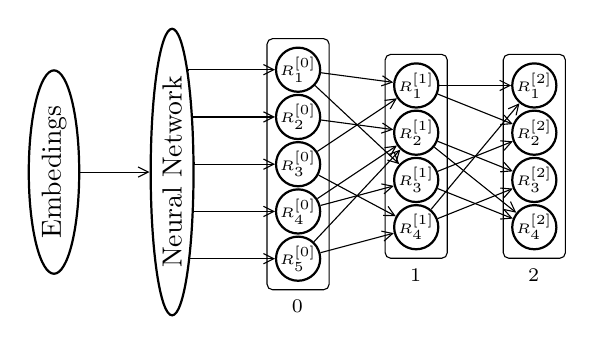
\begin{tikzpicture}
    
    \tikzstyle{enode} = [thick, draw=black, ellipse, inner sep = 2pt,  align=center]
    \tikzstyle{cnode} = [thick, draw=black, circle, inner sep = 0.0pt,  align=center]
    \tikzstyle{nnode} = [thick, rectangle, rounded corners = 0pt,draw,inner sep = 2pt]
    \begin{scope}[xshift=-1cm, yshift=-1.3cm, scale=0.6]
      \node[enode, rotate=90] (em) at (-2.5,0) {Embedings};
      \node[enode, rotate=90] (nn) {Neural Network};
    \end{scope}
    
    % level0 regions
    \begin{scope}[scale=0.6]
      \node[cnode] (r01) at (1, 0) {\tiny$R_1^{[0]}$};
      \node[cnode] (r02) at (1, -1) {\tiny$R_2^{[0]}$};
      \node[cnode] (r03) at (1, -2) {\tiny$R_3^{[0]}$};
      \node[cnode] (r04) at (1, -3) {\tiny$R_4^{[0]}$};
      \node[cnode] (r05) at (1, -4) {\tiny$R_5^{[0]}$};
      \node[label=below:$\Rr_0$, draw,rounded corners = 2pt, inner sep=1mm, fit=(r01) (r05)] {};
    \end{scope}

    \draw[->] (nn.351.9) |- (r01);
    \draw[->] (nn.340) |- (r02);
    \draw[->] (nn.295) |- (r03);
    \draw[->] (nn.210) |- (r04);
    \draw[->] (nn.191) |- (r05);

    \draw[->] (em) -- (nn);


    % level 1 regions
    \begin{scope}[xshift=1.5cm, yshift=-0.2cm, scale=0.6]
      \node[cnode] (r11) at (1, 0) {\tiny$R_1^{[1]}$};
      \node[cnode] (r12) at (1, -1) {\tiny$R_2^{[1]}$};
      \node[cnode] (r13) at (1, -2) {\tiny$R_3^{[1]}$};
      \node[cnode] (r14) at (1, -3) {\tiny$R_4^{[1]}$};
      \node[label=below:$\Rr_1$, draw, rounded corners = 2pt, inner sep=1mm, fit=(r11) (r14)] {};
    \end{scope}

    
    
    % level 1 regions
    \begin{scope}[xshift=3cm, yshift=-0.2cm, scale=0.6]
      \node[cnode] (r21) at (1, 0) {\tiny$R_1^{[2]}$};
      \node[cnode] (r22) at (1, -1) {\tiny$R_2^{[2]}$};
      \node[cnode] (r23) at (1, -2) {\tiny$R_3^{[2]}$};
      \node[cnode] (r24) at (1, -3) {\tiny$R_4^{[2]}$};
      \node[label=below:$\Rr_2$, draw, rounded corners = 2pt, inner sep=1mm, fit=(r21) (r24)] {};
    \end{scope}

    \draw[->] (r01) -- (r11);
    \draw[->] (r03) -- (r11);

    \draw[->] (r02) -- (r12);
    \draw[->] (r04) -- (r12);
    \draw[->] (r05) -- (r12);

    \draw[->] (r01) -- (r13);
    \draw[->] (r04) -- (r13);

    \draw[->] (r03) -- (r14);
    \draw[->] (r05) -- (r14);


    \draw[->] (r11) -- (r21);
    \draw[->] (r14) -- (r21);

    \draw[->] (r11) -- (r22);
    \draw[->] (r13) -- (r22);

    \draw[->] (r12) -- (r23);
    \draw[->] (r14) -- (r23);

    \draw[->] (r12) -- (r24);
    \draw[->] (r13) -- (r24);

    
    
  \end{tikzpicture}
  
  \caption{Illustration of a RENN with three levels of regions ($\Rr_0$, $\Rr_1$, $\Rr_2$).}
  \label{fig:renn-illustration}
  
\end{figure}


In this section, we explain how the proposed region-based energy neural network (RENN) works.
We are interested in finding marginal probabilities such as $p(\bm{x}_R)$. A region belief $b_R(\bm{x}_R)$ is an approximation to $p(\bm{x}_R)$.
Instead of propagating messages as GBP, or directly optimizing with regard to variables ${b_R(\bm{x}_R)}$ of interest, we use the reparameterization technique that is also used by recent works \cite{DBLP:journals/corr/KingmaW13, srikumar-etal-2012-amortizing, NIPS2019_9687, akbayrak2019reparameterization}, to model the values of interest to be the output of a neural network. We then optimize with regard to the parameters of the neural network. This technique is called amortizing.

Note that in RENN, the neural network only needs to directly model the beliefs on root regions $\Rr_0$. The beliefs of non-root regions $\Rr_l,~l>0$ could be obtained from root region beliefs according to the structure of the region graph. This can reduce the number of neural network parameters compared to directly modeling the beliefs of all regions.

\subsection{Inference by RENN}
\label{sec:infer-renn}

For a root region $R^{[0]}\in \Rr_0$, our RENN has a corresponding vector representing its score $\bm{f}(\Gg_R, R^{[0]}; \bm{\omega}) \in \RR^{|{\bm{x}_{R^{[0]}}}| \times K}$, where $\bm{\omega}$ is the parameter of mapping $\bm{f}$ that is modeled by a neural network. We define the predicted belief on the root region node $R^{[0]}$ as
\begin{equation}
  b_{R^{[0]}}(\bm{x}_{R^{[0]}}; \bm{\omega}) := \sigma(\bm{f}(\Gg_R, R^{[0]}; \bm{\omega})), \forall~ {R^{[0]}} \in \Rr,
\end{equation}
where $\sigma(\cdot)$ is the softmax function.

The representation mapping $\bm{f}$ followed by the softmax function in a RENN only needs to directly output the beliefs on root regions $\Rr_0$.
For the rest of the regions $\left\{R \in \Rr \backslash \Rr_0 \right\}$ that are not root regions in the region graph, the RENN computes the belief as
\begin{equation}\label{eq:l-level-beliefs}
  b_{R^{[l]}}(\bm{x}_{R^{[l]}}; \bm{\omega}) := \frac{1}{|\Pp(R^{[l]})|} \sum_{R_p\in  \Pp(R^{[l]})}\sum_{\bm{x}_{R_p}\backslash \bm{x}_{R^{[l]}}} b_{R_p}(\bm{x}_{R_p}; \bm{\omega}),
\end{equation}
where $\Pp(R^{[l]})$ is the set of parent regions of $R^{[l]}$ in the region graph $\Gg_R$. The non-root region belief of RENN defined in this way comes with the intuition of typical iterative belief propagation methods. In BP and its variants, messages are passed to a variable node to reduce the mismatch of beliefs with regard to the variable node, which are sent from this node's neighbors in a factor graph. The message passing iteration of BP or its variants stops when this kind of mismatch with regard to every variable node is eliminated in the factor graph, i.e., it has converged.

In RENN, we directly cast the mismatch between a non-root region belief $b_{R^{[l]}}(\bm{x}_{R^{[l]}}; \bm{\omega})$ and the marginalization from its parent region $\sum_{\bm{x}_{R_p}\backslash \bm{x}_R^{[l]}}b_{R_p}(\bm{x}_{R_p}; \bm{\omega})$ as a penalty in the cost function. As the mismatch penalty is close to zero, the non-root region belief gets close to marginalization calculated from its parent regions. Matching a region's belief with marginalization from its parent regions' beliefs is termed as region belief consistency in the region graph. That is to say, apart from the averaging effect from definition \eqref{eq:l-level-beliefs} itself, a hard-penalty is enforced straightforwardly in our cost.

Different from GBP that minimizes region-based free energy by iterative message-passing, RENN minimizes the region-based free energy by optimizing with regard to the neural network parameter $\bm{\omega}$.
Considering the region belief consistency, we summarize the cost function of RENN to include both the region-based free energy and mismatch penalty on non-root regions. This gives the optimization problem:
\begin{equation}\label{eq:infer-F-all-belief}
  \umin{\bm{\omega}}{F_R(\Bb;\bm{\theta}) + \lambda \sum_{R\in \Rr \backslash \Rr_0} \sum_{R_p \in \Pp(R)} d( b_R, \sum_{\bm{x}_{R_p}\backslash \bm{x}_{R}} b_{R_p}(\bm{x}_{R_p}; \bm{\omega}))},
\end{equation}
where $d(\cdot, \cdot)$ is a distance metric or divergence to measure the mismatch between the beliefs ($L_2$ distance is used in our experiments), $\lambda$ is a positive regularization parameter. To summarize, a RENN takes embedding vectors as input and output beliefs directly by minimizing regularized region-based free energy. Embedding vectors are tunable variables (part of paramter $\bm{w}$), and will be explained in Section~\ref{subsec:exp-setting}, although they are not explicit in the objective function \eqref{eq:infer-F-all-belief}.


\begin{example}
  We demonstrate a toy RENN in this example. As illustrated in Figure~\ref{fig:renn-illustration}, a three-level RENN takes embedding vectors as input and outputs the beliefs on $\Rr_0$ directly. The beliefs in other levels $\{\Rr_1$, $\Rr_2\}$ are computed as in \eqref{eq:l-level-beliefs}. Then the region-based free energy along with the penalty of region belief consistency is minimized with regard to $\bm{\omega}$.
\end{example}

\begin{remark}[Region-based Free Energy and the Partition Function]
  We explained in Section~\ref{chpt2:sec:variational-inference} that Bethe free energy is an approximation to the negative log-partition function, i.e., $-\log{Z(\bm{\theta})}$. This relationship between free energy and partition function similarly exists for RENN.
  After the energy minimization phase as stated in \eqref{eq:infer-F-all-belief}, the minimized region-based free energy $F_R(\Bb^{\ast};\bm{\theta})$ is an approximation to the negative log-partition $-\log{Z(\bm{\bm{\theta}})}$, where $\Bb^{\ast} = \left\{b_R(\bm{x}_R;\bm{\omega}^{\ast})| R \in \Rr \right\}$ with $\bm{\omega}^{\ast}$ as the parameter of RENN after the optimization phase.
\end{remark}

\subsection{Region Graph Construction for RENN}
In this section we detail how to construct the region graph $\Gg_R$ for RENN.
Informally, a region graph can be generated by firstly clustering the nodes in a factor graph in any way and then connect the clusters with directed edges as long as the resulted graph fulfills the Definition~\ref{def:region-graph}. But this does not mean we can rely on an arbitrary region graph to do our inference. Conditions such as \textit{valid} region graph (will be discussed in the following section) and \textit{maxent-normality} \cite{yedida2005constucting,welling2005structured} have been proposed for region graphs. But these conditions do not provide rules for how to construct ''good'' region graphs.
Our approach to this issue is to combine the cluster variation method \cite{PhysRev.81.988,morita1991cluster} with the \textit{tree-robust} condition \cite{gelfand2012generalized} (that was originally developed to improve the accuracy of GBP) to obtain practical region graph construction for RENN.

In what follows, we firstly explain the concept of valid region graphs. Then the method of region graph construction for RENN is detailed.

\subsubsection{Determining the Counting Numbers}
\label{subsec:count-number}
In Definition~\ref{def:region-free-energy}, region-based free energy is defined as a function of counting numbers $\left\{ c_R \right\}$. The counting numbers here are used to balance each region's contribution to the free energy. According to \cite{yedida2005constucting}, the region-base free energy is \text{valid} if the following $1$-balanced conditions holds
\begin{equation}\label{eq:1-ballanced-condition}
  \sum_{R\in\Rr} c_R \delta_{R}(i)  = 1, \forall~ \mathrm{node}~ i~~ \mathrm{in} ~~\Gg_F,
\end{equation}
where $\delta_{R}(i)$ is the indicator function, equal to $1$ if and only if node $i$ defined in factor graph $\Gg_F$ falls in the region $R$ of the region graph $\Gg_R$ and equal to $0$ otherwise. Note that node $i$ can be either a variable or factor node here. It can be seen that each node would be counted exactly once if the condition \eqref{eq:1-ballanced-condition} holds.

Given a region graph $\Gg_R$, the counting numbers $\left\{ c_R \right\}$ can be constructed recursively as
\begin{equation}
  c_R = 1 - \sum_{R_i \in \Aa(R)} c_{R_i}, \forall R,
\end{equation}
where $\Aa(R)$ denotes the ancestor set of region node $R$ in $\Gg_R$. This rule means the counting numbers of root regions are always $1$, since they do not have any ancestors.


\subsubsection{Generating Graph by Cluster Variation Method}
\label{sec:cluster-variation-method}

The cluster variation method was introduced by Kikuchi and other physicists \cite{PhysRev.81.988,morita1991cluster}, which started with the intuition of approximating free energy by using larger sets of variable nodes instead of the single-node factorization in mean field approximation.

The cluster variation method starts with the root regions $\Rr_0$. There are two requirements for $\Rr_0$: i) every variable node $i$ of factor graph $\Gg_F$ is included in at least one region $R^{[0]}\in\Rr_0$; ii) there should be no region $R^{[0]}\in \Rr_0$ being a subregion of any other region in $\Rr_0$.
With $\Rr_0$ ready, the other sets of regions are generated hierarchically. To construct level-$1$ regions $\Rr_1$ from $\Rr_0$, we find all the intersections between regions in $\Rr_0$, but omit any that are subregion of other intersection regions. Then level-$2$ regions $\Rr_2$ can be similarly constructed from $\Rr_1$. Assume there are $L$ such sets, then $\Rr = \Rr_0 \cup \Rr_1 \cup \cdots \cup \Rr_{L-1}$. The construction rule can be formulated as
\begin{align}
  \Rr_l = &\{ R^{[l]}_i := R^{[l-1]}_j \cap R^{[l-1]}_k | R^{[l]}_i \not\subset R^{[l]}_n,~ \forall i \neq n, \nonumber \\
          &R^{[l-1]}_j, R^{[l-1]}_k \in \Rr_{l-1} , j\neq k\}, l=1, 2, \cdots, L-1.
\end{align}

With the hierarchical region sets built, we need to draw the edges. The directed edges are always connected from regions in $\Rr_{l-1}$ to these in $\Rr_{l}$. For one region $R^{[l]}$ in $\Rr_l$, a directed edge is drawn from any superregion of $R^{[l]}$ in $\Rr_l$. This can be represented as
\begin{align}
  \Ee = \{ e := (R^{[l-1]}, R^{[l]}) | R^{[l]} \subset R^{[l-1]}, R^{[l]} \in \Rr_l, R^{[l-1]} \in \Rr_{l-1} , \forall l\}.
\end{align}



\subsubsection{Root Region Construction}
\label{sec:criteria-root-regions}
In the previous section, we detailed the region graph construction steps by cluster variation method, starting from $\Rr_0$. In this section, we explain how to build the root region set $\Rr_0$. This is important since it totally decides from which we start building a region graph.
We follow the path of \cite{welling2005structured, gelfand2012generalized} for this issue.
Specifically, we use the \textit{tree-robust} condition \cite{gelfand2012generalized} to build the root regions for our RENN. These root regions are then used to grow the other hierarchical levels of the region graph by the cluster variation method. The tree-robust condition was developed originally for GBP to gain better approximations. GBP has better accuracy on tree-robust graphs than on non-tree-robust graphs. We will show in our experiment in Section~\ref{chpt4:sec:experiments} that RENN outperforms GBP even in tree-robust graphs. 


To explain the concept of \textit{tree-robust}, we need to explain the concepts of \textit{cycle basis} and \textit{tree exact}, based on which the tree-robust is defined.
\begin{definition}\label{apdix:def:cycle-basis}
  A \textit{cycle basis} of the cycle space of a graph $\Gg$ is a
  set of simple cycles $\Cc\Bb =\left\{ C_1, C_2, \cdots, C_{\mu}
  \right\}$ such that for every cycle $C$ in graph $\Gg$, there
  exists a unique subset $\Cc\Bb_{C} \subseteq \Cc\Bb$ such that the
  set of edges appearing an odd number of times in $\Cc\Bb_C$ comprise the cycle $C$.
\end{definition}
\begin{definition}\label{apdix:def:tree-exact}
  Let $T$ be a spanning tree of graph $\Gg$. A cycle basis $\Cc\Bb$ is \textit{tree exact} with regard to $T$ if there exists an ordering $\pi$ of the cycles in $\Cc\Bb$ such that
  \begin{equation*}
    \left\{ C_{\pi(i)} \backslash C_{\pi(1)} \cup C_{\pi(2)} \cup \cdots \cup C_{\pi(i-1)} \right\} \neq \emptyset~~\mathrm{for}~~ i=2,\cdots, \mu.
  \end{equation*}
\end{definition}
Definition~\ref{apdix:def:tree-exact} tells us that if a cycle basis is tree exact with regard to $T$ and ordered properly, there is at least one edge of $C_{\pi}$ that has not appeared in any cycles preceding it, and meanwhile this edge does not appear in the spanning tree $T$.
With the above concepts, we are ready to give the definition of tree-robust.
\begin{definition}
  A cycle basis $\Cc\Bb$ is tree-robust if it is tree exact with regard to all spanning trees of $\Gg$.
\end{definition}


We use two theorems from \cite{gelfand2012generalized} for choosing cycle basis in two specific graph classes, i.e. planar graphs and complete graphs. A planar graph is a graph that can be embedded in the two-dimensional plain (it can be drawn on the plane in such a way that its edges intersect only at their nodes). In a complete graph, every pair of distinct nodes is connected by a unique edge.

\begin{theorem}\label{thm:planar-tree-robust}
  In a planar graph $\Gg$, the cycle basis comprised of the faces of the graph $\Gg$ is tree-robust.
\end{theorem}

\begin{theorem}\label{thm:complete-tree-robust}
  In a complete graph $\Gg$, construct a cycle basis as follows. Choose a node $i$ as the root. Create a 'star' spanning tree rooted at $i$. Then construct cycles of form $(i,j,k)$ from each off-tree edge $(j,k)$. The constructed basis is tree-robust.
\end{theorem}

Tree-robust root regions can also be constructed for general graphs, which can be seen as an extension from Theorem~\ref{thm:planar-tree-robust} and \ref{thm:complete-tree-robust}. For general graph case, it basically is to find a subgraph that is a planar or compote graph, and then extract the corresponding tree-robust basis, after which extra cycles are added in by following Algorithm~\ref{apdix:alg:root-region-general-graph}. To be more specific, the Algorithm~\ref{apdix:alg:root-region-general-graph} returns a partially tree-robust basis, since tree-robust condition for a general graph requires inspecting all subsets of cycles in a candidate basis, which is usually prohibitive. 
\begin{algorithm}[tb]
  \caption{Construct Root Regions from General Graphs.}
  \label{apdix:alg:root-region-general-graph}
  \begin{algorithmic}
    \STATE {\bfseries Input:} Pairwise Markov random field $p(\bm{x})$
    \STATE Draw the factor graph $\Gg_F$ of $p(\bm{x})$
    \STATE Obtain graph $\Gg$ by preserving the variable nodes as they are and converting the factor nodes of $\Gg_F$ into edges, i.e., the undirected graph of MRF representation
    \STATE Find the subgraph $\Gg_s$ of $\Gg$, such that $\Gg_s$ is planar or complete graph
    \STATE Add the tree-robust basis $\Cc\Bb(\Gg_s)$ of $\Gg_s$ into $\Rr_0$
    \STATE Marked all nodes as \textit{visited} and edged as \textit{used} in $\Gg_s$
    \REPEAT
    \STATE Choose an \textit{unused} edge $e = (s,t)$ from a \textit{visited} node $s$
    \IF{$t$ is visited}
    \STATE Set $\mathrm{path_1} = e$
    \STATE Find the shortest path $\mathrm{path}_2$ from $s$ to $t$
    via \textit{used} edges
    \ELSE
    \STATE Find a path from $s$ to a \textit{visited} $u$ that
    contains edge $e$, this path is set as $\mathrm{path_1}$.
    \STATE Find the shortest path $\mathrm{path}_2$ from $s$ to $u$
    via \textit{used} edges
    \ENDIF
    \STATE Add cycle $C$ consisting of $\mathrm{path_1}$ and
    $\mathrm{path_2}$ to $\Rr_0$.
    \STATE Mark all nodes as \textit{visited} and edges as
    \textit{used} in $C$
    \UNTIL{$\nexists$ \textit{unused} edge $e = (s,t)$ from a
      \textit{visited} node $s$}
  \end{algorithmic}
\end{algorithm}





\section{Experimental Results}\label{chpt4:sec:experiments}

We conducted a series of experiments to validate the proposed RENN model. The experiments are designed to verify RENN in inference problems. 
Apart from the inference experiments, we also carried out the MRF model learning experiments. Analysis and experiments on MRF learning are discussed in Chapter~\ref{chpt5:undirecteLearning}.



\begin{sidewaystable}[ph!]
  \caption{Inference on grid graph ($\gamma=0.1$). $\ell_1$ error and correlation $\rho$ between true and approximate marginals, and $\log{Z}$ error.}
  \label{table:infer-grid-gamma0.1}
  \begin{center}
    \begin{small}
      \begin{tabular}{lcccccccc}
        \toprule
        Metric & $n$ & Mean Field & Loopy BP & Damped BP & GBP & Inference Net & RENN \\
        \midrule
        \multirow{4}{*}{\begin{tabular}[x]{@{}c@{}}$\ell_1$\\error \end{tabular} }
               &    25   &$0.271 \pm 0.051$ &  $0.086 \pm 0.078$ & $0.084 \pm 0.076$ & $0.057 \pm 0.024$ & $0.111 \pm 0.072$ & \textbf{0.049} $\pm$ 0.078 \\
        
               &    100   & $0.283 \pm 0.024$ &  $0.085 \pm 0.041$ & $0.062 \pm 0.024$ & $0.064 \pm 0.019$ & $0.074 \pm 0.034$ & \textbf{0.025} $\pm$ 0.011 \\
        
               &    225   & $0.284 \pm 0.019$ &  $0.100 \pm 0.025$ & $0.076 \pm 0.025$ & $0.073 \pm 0.013$ & $ 0.073 \pm 0.012$ & \textbf{0.046} $\pm$ 0.011 \\
        
               &    400   & $0.279 \pm 0.014$ &  $0.110 \pm 0.016$ & $0.090 \pm 0.016$ & $0.079 \pm 0.009$ & $ 0.083 \pm 0.009$ & \textbf{0.061} $\pm$ 0.009 \\

        \midrule
        \multirow{4}{*}{\begin{tabular}[x]{@{}c@{}}Corre-\\lation\\ $\rho$ \end{tabular}}
               &   25    & 0.633 $\pm$ 0.197  &  0.903 $\pm$ 0.114  &  0.905 $\pm$ 0.113  &  0.923 $\pm$ 0.045  &  0.866$\pm$ 0.117 &  \textbf{0.951} $\pm$ 0.112 \\
        
               &   100   & 0.582 $\pm$ 0.112  &  0.827 $\pm$ 0.134  &  0.902 $\pm$ 0.059  &  0.899 $\pm$ 0.043  &  0.903$\pm$ 0.049 &   \textbf{0.983} $\pm$ 0.012 \\
        
               &   225   & 0.580 $\pm$ 0.080  &  0.801 $\pm$ 0.078  &  0.863 $\pm$ 0.088  &  0.869 $\pm$ 0.037  & 0.873 $\pm$ 0.037 &  \textbf{0.949} $\pm$ 0.022 \\
        
               &   400   & 0.596 $\pm$ 0.054  &  0.779 $\pm$ 0.059  &  0.822 $\pm$ 0.047  &  0.852 $\pm$ 0.024  & 0.841 $\pm$ 0.028 &  \textbf{0.912} $\pm$ 0.025 \\

        \midrule
        \multirow{4}{*}{\begin{tabular}[x]{@{}c@{}}$\log{Z}$ \\error\end{tabular}}
               &   25    & 2.512 $\pm$ 1.060  &  0.549 $\pm$ 0.373  &  0.557 $\pm$ 0.369  &  \textbf{0.169} $\pm$ 0.142  &  0.762 $\pm$ 0.439  &  0.240 $\pm$ 0.140 \\

               &  100    & 13.09 $\pm$ 2.156  &  1.650 $\pm$ 1.414  &  1.457 $\pm$  1.365 &  \textbf{0.524} $\pm$ 0.313  &  2.836 $\pm$ 2.158  & 1.899 $\pm$ 0.495 \\

               &  225    & 29.93 $\pm$ 4.679  &  3.348 $\pm$ 1.954  &  3.423 $\pm$ 2.157  &  \textbf{1.008} $\pm$ 0.653  &  3.249 $\pm$ 2.058  & 4.344 $\pm$ 0.813  \\

               &  400    & 51.81 $\pm$ 4.706  &  5.738 $\pm$ 2.107  &  5.873$\pm$ 2.211   &  \textbf{1.750} $\pm$ 0.869  &  3.953 $\pm$ 2.558  & 7.598 $\pm$ 1.146 \\
        
               % \midrule
               % \multirow{4}{*}{Time}
               % &   25   &  0.259 $\pm$ 0.076  &  2.990 $\pm$ 4.563  &  1.591 $\pm$ 0.609  &  6.817 $\pm$ 0.339  &  5.253 $\pm$ 1.189  &  5.828 $\pm$ 2.372  \\
               % &  100   &  1.290 $\pm$ 0.205  &  57.10 $\pm$ 25.64 &  28.70 $\pm$ 24.62 & 46.89$ \pm$ 1.365 & 22.05 $\pm$ 10.53  & 22.63 $\pm$ 6.202 \\

               % &  225   &  3.838 $\pm$ 1.015  &  184.1 $\pm$ 3.648  &  124.2 $\pm$ 68.70  &  131.1 $\pm$ 3.440  &  36.43 $\pm$ 2.087  & 51.82 $\pm$ 2.431 \\

               % &  400   &  7.908 $\pm$ 1.508  & 335.3 $\pm$ 12.83   &  326.9 $\pm$ 27.56  &  253.7 $\pm$ 11.00   &  69.54 $\pm$ 5.140  & 103.9 $\pm$ 8.379 \\
        
        
        \bottomrule
      \end{tabular}
    \end{small}
  \end{center}
\end{sidewaystable}

\begin{sidewaystable}[ph!]
  \caption{Inference on grid Graph. ($\gamma=1$)}
  \label{table:infer-grid-gamma1.0}
  \begin{center}
    \begin{small}
      
      \begin{tabular}{lcccccccc}
        \toprule
        Metric & $n$ & Mean Field & Loopy BP & Damped BP & GBP & Inference Net & RENN \\
        \midrule
        \multirow{4}{*}{L1}
               & 25   &  0.131 $\pm$ 0.080  &  \textbf{0.022} $\pm$ 0.017  &  0.022 $\pm$ 0.018  &  0.137 $\pm$ 0.026  &  0.043 $\pm$ 0.017  &  0.027 $\pm$ 0.014 \\
               & 100  &  0.130 $\pm$ 0.041  &  0.025 $\pm$ 0.014  &  0.025 $\pm$ 0.014  &  0.146 $\pm$ 0.020  &  0.046 $\pm$ 0.009  &  \textbf{0.017} $\pm$ 0.002  \\

               &225   &  0.135 $\pm$ 0.024  &  0.024 $\pm$ 0.010  &  0.023 $\pm$ 0.009  &  0.154 $\pm$ 0.012  &  0.052 $\pm$ 0.010  &  \textbf{0.017} $\pm$ 0.003 \\

               &400   &  0.131 $\pm$ 0.020  &  0.020 $\pm$ 0.003  &  0.020 $\pm$ 0.003  &  0.158 $\pm$ 0.007  &  0.052 $\pm$ 0.007  &  \textbf{0.017} $\pm$ 0.001  \\
        
        
        
        \midrule
        \multirow{4}{*}{\begin{tabular}[x]{@{}c@{}}Corre-\\lation\end{tabular}}
               & 25   &  0.849 $\pm$ 0.159  &  \textbf{0.992} $\pm$ 0.011  &  0.991 $\pm$ 0.012  &  0.798 $\pm$ 0.088  &  0.980 $\pm$ 0.015  & 0.988 $\pm$ 0.025  \\
               & 100  &  0.841 $\pm$ 0.087  &  0.988 $\pm$ 0.013  &  0.988 $\pm$ 0.012  &  0.788 $\pm$ 0.051  &  0.976 $\pm$ 0.013  &  \textbf{0.997} $\pm$0.001 \\

               & 225  &  0.824 $\pm$ 0.057  &  0.989 $\pm$ 0.010  &  0.990 $\pm$ 0.010  &  0.764 $\pm$ 0.022  &  0.966 $\pm$ 0.016  &  \textbf{0.996} $\pm$ 0.001 \\
        
               & 400  &  0.828 $\pm$ 0.043  &  0.993 $\pm$ 0.002  &  0.993 $\pm$ 0.002  &  0.759 $\pm$ 0.018  &  0.967 $\pm$ 0.013  &  \textbf{0.997} $\pm$ 0.001  \\

        \midrule
        \multirow{4}{*}{\begin{tabular}[x]{@{}c@{}}$\log{Z}$ \\error\end{tabular}}
               & 25  &  2.113 $\pm$ 1.367  &  \textbf{0.170} $\pm$ 0.199  &  0.194 $\pm$ 0.188  &  0.605 $\pm$ 0.611  &  2.214 $\pm$ 0.775  &  0.649 $\pm$ 0.363  \\

               &100  &  8.034 $\pm$ 2.523  &  \textbf{0.372} $\pm$ 0.427  &  0.415 $\pm$ 0.422  &  1.545 $\pm$ 1.081  &  11.14 $\pm$ 0.954  &  3.129 $\pm$ 0.520  \\

               &225  &  17.923 $\pm$ 3.474 &  0.952 $\pm$ 1.037  &  \textbf{0.917} $\pm$ 0.922  &  3.143 $\pm$ 2.122  &  25.55 $\pm$ 2.025  &  7.473 $\pm$ 0.906  \\

               &400  &  31.74 $\pm$ 4.766          &  \textbf{0.919} $\pm$ 0.684   &  1.011 $\pm$ 0.685  &  3.313 $\pm$ 1.872  &  46.61 $\pm$ 3.094  &  12.77 $\pm$ 0.991  \\

        
               % \midrule
               % \multirow{4}{*}{Time}
               % & 25  &  0.281 $\pm$ 0.129  &  0.937 $\pm$ 0.442  &  1.253 $\pm$ 0.403  &  6.982 $\pm$ 0.260  &  5.146 $\pm$ 0.398  &  5.341 $\pm$ 1.368  \\

               % & 100 &  1.219 $\pm$ 0.314  &  6.339 $\pm$ 3.965  &  6.948 $\pm$ 1.664  &  49.64 $\pm$ 1.301  &  21.59 $\pm$ 4.703  &  31.79 $\pm$ 15.51  \\
        
               % &125  &  3.539 $\pm$ 1.107  &  33.09 $\pm$ 48.62  &  17.85 $\pm$ 4.765  &  127.1 $\pm$ 3.547  &  56.99 $\pm$ 4.625  &  94.05 $\pm$ 38.64  \\


               % &400  &  6.313 $\pm$ 1.465  &  49.26 $\pm$ 65.20  &  33.07 $\pm$ 8.777  &  
               % 255.1 $\pm$ 10.13  &  157.3 $\pm$ 34.04  &  172.58 $\pm$ 27.08  \\
        \bottomrule
      \end{tabular}

    \end{small}
  \end{center}
\end{sidewaystable}


\subsection{Experiment Setting and Evaluation Metrics}
\label{subsec:exp-setting}
Without loss of generality, our experiments are carried out on binary pairwise MRF (Ising model). This gives us $p(\bm{x}; \bm{\theta}) = \frac{1}{Z(\bm{\theta})}\exp{(\sum_{(i,j)\in \Ee_F} J_{ij} x_i x_j + \sum_{i\in \Vv}h_i x_i)}$, $\bm{x} \in \{-1, 1\}^{N}$, where $J_{ij}$ is the pairwise log-potential between node $i$ and $j$, $h_i$ is the node log-potential for node $i$. Then $\bm{\theta} = \left\{ J_{ij}, h_i| (i,j) \in \Ee_F, i,j \in \Vv \right\}$. $J_{ij}$ is always sampled from standard normal distribution, i.e. $J_{ij}\sim \mathsf{N}(0,1)$, meanwhile $h_i \sim \mathsf{N}(0, \gamma^{2})$ with varying $\gamma$ in different experiment cases.

In the inference experiments, we are interested in how well beliefs from RENN approximate true marginal distributions of $p(\bm{x};\bm{\theta})$. We quantify this by both the $\ell_1$ error ($\ell_1$-norm distance) and Pearson correlation coefficient $\rho$, between true marginals and beliefs of RENN. The marginal evaluations include both $p(x_i)$ and $p(x_i,x_j)$. In addition, we also quantify the $\log{Z}$ error as the absolute difference between true partition function and an approximated value, i.e., the region-based free energy for RENN or GBP while a counterpart free energy form for mean field or loopy BP as explained in Section~\ref{chpt2:sec:variational-inference}.

In all experiments, for each evaluation of RENN, mean field, (loopy) BP \cite{mooij2007sufficient}, damped BP \cite{Pretti2005damping} with damping factor $0.5$, and GBP \cite{yedida2005constucting} as benchmarks, are all evaluated on the same MRF, which are then compared with RENN. Additionally, a recent neural network benchmark model, saddle-point Inference Net \cite{NIPS2019_9687} targeting the Bethe free energy, is also used as a comparison. To make the comparison with Inference Net fair, RENN and Inference Net use the same neural network structures and hidden dimensions. Each variable $x_i$ is associated with a learnable embedding vector $\bm{e}_i$. A transform layer \cite{AshishNIPS2017_7181} consumes $\bm{e}_i$ and outputs a hidden representation $\bm{h}_i$. The transform layer is shared by all embeddings. Then an affine layer followed by softmax consumes $[\bm{h}_1, \cdots, \bm{h}_N]$ and outputs beliefs.

\subsection{Inference on Grid Graphs}

We first evaluate how well RENN can estimate the marginal distributions, compared with benchmark algorithms/models, with regard to marginal $\ell_1$ errors and Pearson correlation $\rho$, for different graph size $n$ and standard deviation $\gamma$ of $\{h_i\}$. At each evaluation for a given size $n$, $20$ MRFs are generated by sampling $\{J_{ij}\}$ and $\{h_i\}$. Then RENN and other candidate algorithms perform inference on these MRFs. The $\ell_1$ error and correlation $\rho$ between true and estimated marginal distributions are evaluated. The $\log{Z}$ error is also recorded.
Experiments are carried out in large and small standard deviation of $\{h_i\}$ ($\gamma=0.1$, $\gamma=1$), which reflects the relative strength of standalone node log-potentials to pairwise log-potentials. The results are reported as 'mean $\pm$ standard deviation' in tables.

\begin{table}[tp!]
  \caption{Inference with the \textit{infinite face} on grid, $n=25$.}
  \label{tab:infer-infinite-face}
  \begin{center}
    \begin{small}
      
      \begin{tabular}{llcc}
        \toprule
        $\gamma$ & Metric & GBP & RENN \\
        \midrule
        \multirow{3}{*}{0.1}
                 & $\ell_1$ Error & 0.061 $\pm$ 0.025 & \textbf{0.025} $\pm$ 0.020 \\

                 & $\rho$   & 0.913 $\pm$ 0.049  &  \textbf{0.984} $\pm$ 0.021  \\
                 & $\log{Z}$ Error & 3.564 $\pm$ 2.823  &  0.384 $\pm$ 0.223  \\
        \midrule
        \multirow{3}{*}{1}
                 & $\ell_1$ Error & 0.145 $\pm$ 0.028  & \textbf{0.016} $\pm$ 0.010 \\

                 & $\rho$   & 0.783 $\pm$ 0.091  &  \textbf{0.995} $\pm$ 0.010 \\
                 & $\log{Z}$ Error & 0.825 $\pm$ 0.841  & 0.364 $\pm$ 0.201 \\
        
        \bottomrule
      \end{tabular}

    \end{small}
  \end{center}
\end{table}







\begin{sidewaystable}[ph!]
  \caption{Inference on complete graph of size $9$.}
  \label{tab:infer-full-n9}
  \begin{center}
    \begin{small}
      
      \begin{tabular}{lcccccccc}
        \toprule
        Metric & $\gamma$ & Mean Field & Loopy BP & Damped BP & GBP & Inference Net & RENN \\
        \midrule
        \multirow{4}{*}{\begin{tabular}[x]{@{}c@{}}$\ell_1$\\error\end{tabular}}
        % pen1
               & 0.1   &  0.294 $\pm$ 0.061  &  0.120 $\pm$ 0.038  &  0.118 $\pm$ 0.034  &   0.237 $\pm$ 0.061  &  \textbf{0.109} $\pm$ 0.025  &  0.130 $\pm$ 0.085  \\

               % pen2
               & 1     &  0.233 $\pm$ 0.133  &  0.200 $\pm$ 0.098  &  0.201 $\pm$ 0.098  &  0.246 $\pm$ 0.135  &  0.196 $\pm$ 0.061  &  \textbf{0.137} $\pm$ 0.117  \\

               % pen3
               & 2     &  0.187 $\pm$ 0.131  &  0.176 $\pm$ 0.114  &  0.177 $\pm$ 0.113  &  0.247 $\pm$ 0.117  &  0.182 $\pm$ 0.084  &  \textbf{0.067} $\pm$ 0.045  \\

               % pen3
               & 3     &  0.155 $\pm$ 0.120  &  0.145 $\pm$ 0.112  &  0.146 $\pm$ 0.112  &  0.204 $\pm$ 0.107  &  0.152 $\pm$ 0.079  &  \textbf{0.060} $\pm$ 0.038  \\

               % pen3
               & 4     &  0.124 $\pm$ 0.115  &  0.120 $\pm$ 0.103  &  0.121 $\pm$ 0.102  &  0.194 $\pm$ 0.076  &  0.129 $\pm$ 0.071  &  \textbf{0.051} $\pm$ 0.050  \\

        
        \midrule
        \multirow{4}{*}{\begin{tabular}[x]{@{}c@{}}Corre-\\lation\\$\rho$\end{tabular}}
               & 0.1   & 0.262 $\pm$ 0.177  &  0.695 $\pm$ 0.104  &  0.698 $\pm$ 0.099  &  0.446 $\pm$ 0.196  &   0.720 $\pm$ 0.065  &  \textbf{0.741} $\pm$ 0.220  \\

               & 1     & 0.465 $\pm$ 0.349  &  0.538 $\pm$ 0.292  &  0.538 $\pm$ 0.292  &  0.461 $\pm$ 0.331  &  0.639 $\pm$ 0.159   &  \textbf{0.769} $\pm$ 0.313  \\

               &  2    & 0.587 $\pm$ 0.300  &  0.619 $\pm$ 0.284  &  0.619 $\pm$ 0.282  &  0.457 $\pm$ 0.257  &   0.645 $\pm$ 0.175  &  \textbf{0.929} $\pm$ 0.118  \\

               &  3    & 0.657 $\pm$ 0.289  &  0.697 $\pm$ 0.267  &  0.697 $\pm$ 0.265  &  0.582 $\pm$ 0.218  &  0.697 $\pm$ 0.162   &  \textbf{0.936} $\pm$ 0.076  \\

               &  4    & 0.758 $\pm$ 0.257  &   0.778 $\pm$ 0.221 &  0.776 $\pm$ 0.221  &  0.597 $\pm$ 0.177  &  0.753 $\pm$ 0.178   &  \textbf{0.941} $\pm$ 0.099  \\
        
        
        
        \midrule
        \multirow{4}{*}{\begin{tabular}[x]{@{}c@{}}$\log{Z}$ \\error\end{tabular}}
               & 0.1  & 8.402 $\pm$ 4.369  &  34.61 $\pm$ 2.439  &  34.74 $\pm$ 2.195  &  \textbf{1.763} $\pm$ 1.176  &  35.46 $\pm$ 1.651  &  3.171 $\pm$ 1.259   \\

               &  1   & 6.473 $\pm$ 3.737  &  45.91 $\pm$ 6.888  &  45.96 $\pm$ 6.927  &  \textbf{1.826} $\pm$ 2.024  &  51.87 $\pm$ 6.150  &  2.796 $\pm$ 1.194  \\
        
               &  2   & 5.830 $\pm$ 2.979  &  75.35 $\pm$ 14.58  &  75.46 $\pm$ 14.57  &  3.080  $\pm$ 2.958  &  81.23 $\pm$ 12.939 &  \textbf{2.577} $\pm$ 1.845  \\

               &  3   & 4.401 $\pm$ 2.522  &  111.0 $\pm$ 22.20  &  111.1 $\pm$ 22.17  &  3.205 $\pm$ 3.720  &  116.1 $\pm$ 19.76  &  \textbf{2.645} $\pm$ 1.507  \\

               &  4   & 3.037 $\pm$ 2.122  &  142.9 $\pm$ 25.58  &  143.1 $\pm$ 25.56  &  5.167 $\pm$ 5.249  &  147.2 $\pm$ 23.38  &  \textbf{1.820} $\pm$ 1.306  \\

               % \midrule
               % \multirow{4}{*}{Time}
               % & 0.1  &  0.270 $\pm$ 0.096  &  0.490 $\pm$ 0.315  &  0.590 $\pm$ 0.544  & 3.023 $\pm$ 0.122  &  4.644 $\pm$ 0.326  &  4.979 $\pm$ 1.612  \\

               % &  1   & 0.186 $\pm$ 0.059   &  0.302 $\pm$ 0.072  &  0.501 $\pm$ 0.112  &  2.854 $\pm$ 0.098  &  4.330 $\pm$ 0.423  &  4.905 $\pm$ 1.815  \\

               % &  2   & 0.111 $\pm$ 0.031   &  0.178 $\pm$ 0.028  &  0.315 $\pm$ 0.048  &  2.722 $\pm$ 0.099  &  4.529 $\pm$ 0.569  &  5.329 $\pm$ 1.725  \\

               % &  3   & 0.112 $\pm$ 0.072   &  0.155 $\pm$ 0.025  &  0.281 $\pm$ 0.057  &  2.671 $\pm$ 0.131  &  4.667 $\pm$ 1.217  &  4.477 $\pm$ 2.076  \\

               % &  4   & 0.098 $\pm$ 0.039   &  0.141 $\pm$ 0.026  &  0.279 $\pm$ 0.062  &  2.731 $\pm$ 0.110  &  5.091 $\pm$ 1.798  &  4.309 $\pm$ 1.152  \\
        
        \bottomrule
      \end{tabular}
      
    \end{small}
  \end{center}
\end{sidewaystable}

\begin{sidewaystable}[ph!]
  \caption{Inference on complete graph of size $16$.}
  \label{tab:infer-full-n16}
  % \vskip -0.05in
  \begin{center}
    \begin{small}

      \begin{tabular}{lcccccccc}
        \toprule
        Metric & $\gamma$ & Mean Field & Loopy BP & Damped BP & GBP & Inference Net & RENN \\
        \midrule
        \multirow{4}{*}{\begin{tabular}[x]{@{}c@{}}$\ell_1$-\\error\end{tabular}}
        % pen3
               & 0.1   &  0.303 $\pm$ 0.056  &  0.176 $\pm$ 0.039  &  0.174 $\pm$ 0.038  &  0.244 $\pm$ 0.047  &  0.174 $\pm$ 0.044  &  \textbf{0.169} $\pm$ 0.052  \\

               % pen2
               &  1    &  0.273 $\pm$ 0.086  &  0.239 $\pm$ 0.059  &  0.239 $\pm$ 0.059  &  0.260 $\pm$ 0.086  &  0.249 $\pm$ 0.067  &  \textbf{0.181} $\pm$ 0.092  \\
        
               % pen2
               &  2    &  0.231 $\pm$ 0.079  &  0.222 $\pm$ 0.064  &  0.221 $\pm$ 0.064  &  0.249 $\pm$ 0.078  &  0.232 $\pm$ 0.069  &  \textbf{0.170} $\pm$ 0.109  \\

               % pen3
               &  3    &  0.218 $\pm$ 0.042  &  0.204 $\pm$ 0.038  &  0.204 $\pm$ 0.038  &  0.247 $\pm$ 0.065  &  0.213 $\pm$ 0.051  &  \textbf{0.138} $\pm$ 0.106  \\

               % pen1
               &  4    &  0.197 $\pm$0.049   &  0.181 $\pm$ 0.035  &  0.180 $\pm$ 0.034  &  0.210 $\pm$ 0.070  &  0.174 $\pm$ 0.030  &  \textbf{0.125} $\pm$ 0.050  \\
        
        
        \midrule
        \multirow{4}{*}{\begin{tabular}[x]{@{}c@{}}Corre-\\lation\\$\rho$\end{tabular}}
               & 0.1   &  0.231 $\pm$ 0.196  &  0.509 $\pm$ 0.056  &  0.510 $\pm$ 0.055  &  0.316 $\pm$ 0.207  &  0.506 $\pm$ 0.063  &  \textbf{0.539} $\pm$ 0.235  \\

               &  1    &  0.381 $\pm$ 0.255  &  0.514 $\pm$ 0.185  &  0.515 $\pm$ 0.185  &  0.445 $\pm$ 0.223  &  0.533 $\pm$ 0.150  &  \textbf{0.756} $\pm$ 0.187  \\


               &  2    &  0.535 $\pm$ 0.207  &  0.569 $\pm$ 0.180  &  0.570 $\pm$ 0.179  &  0.480 $\pm$ 0.186  &  0.559 $\pm$ 0.176  &  \textbf{0.750} $\pm$ 0.261  \\


               &  3    &  0.586 $\pm$ 0.142  &  0.618 $\pm$ 0.134  &  0.619 $\pm$ 0.134  &  0.502 $\pm$ 0.144  &  0.613 $\pm$ 0.128  &  \textbf{0.853} $\pm$ 0.159  \\

               &  4    &  0.622 $\pm$ 0.166  &  0.658 $\pm$ 0.133  &  0.660 $\pm$ 0.132  &  0.564 $\pm$ 0.165  &  0.693 $\pm$ 0.060  &  \textbf{0.868} $\pm$ 0.053  \\

        
        \midrule
        \multirow{4}{*}{\begin{tabular}[x]{@{}c@{}}$\log{Z}$ \\error\end{tabular}}
               & 0.1   &  24.45 $\pm$ 7.560  &  143.7 $\pm$ 9.297  &  145.5 $\pm$ 6.096  &  166.3 $\pm$ 11.98  &  148.5 $\pm$ 3.522  &  \textbf{12.57} $\pm$ 3.689  \\

               &  1    &  20.66 $\pm$ 5.451  &  178.7 $\pm$ 22.18  &  178.9 $\pm$ 21.88  &  153.3 $\pm$ 25.29  &  213.6 $\pm$ 12.75  &  \textbf{14.41} $\pm$ 4.135  \\

               &  2    &  16.04 $\pm$ 4.352  &  296.3 $\pm$ 44.41  &  296.9 $\pm$ 44.24  &  116.9 $\pm$ 32.72  &  335.1 $\pm$ 32.86  &  \textbf{13.37} $\pm$ 4.531  \\


               &  3    &  13.87 $\pm$ 6.554  &  432.7 $\pm$ 66.44  &  433.4 $\pm$ 66.30  &  100.2 $\pm$ 39.62  &  462.9 $\pm$ 53.61  &  \textbf{12.56} $\pm$ 6.046  \\

               &  4    &  \textbf{10.74} $\pm$ 7.385  &  565.7 $\pm$ 73.33  &  566.1 $\pm$ 73.13  &  106.0 $\pm$ 54.43  &  588.3 $\pm$ 62.58  &  14.72 $\pm$ 4.155  \\
        

               % \midrule
               % \multirow{4}{*}{Time}
               % & 0.1   &  0.555 $\pm$ 0.135  &  1.705 $\pm$ 1.256  &  1.428 $\pm$ 0.400  &  13.68 $\pm$ 0.432  &  12.63 $\pm$ 0.592  &  15.26 $\pm$ 4.759  \\

               % &  1    &  0.457 $\pm$ 0.103  &  0.777 $\pm$ 0.167  &  1.285 $\pm$ 0.190  &  14.29 $\pm$ 0.487  &  12.45 $\pm$ 0.603  &  16.16 $\pm$ 5.695  \\

               % &  2    &  0.424 $\pm$ 0.101  &  0.630 $\pm$ 0.096  &  1.143 $\pm$ 0.196  &  14.76 $\pm$ 0.512  &  15.04 $\pm$ 1.106  &  14.74 $\pm$ 4.606  \\

               % &  3    &  0.377 $\pm$ 0.114  &  0.567 $\pm$ 0.118  &  1.084 $\pm$ 0.254  &  14.49 $\pm$ 0.392  &  15.62 $\pm$ 1.218  &  13.40 $\pm$ 3.070  \\

               % &  4    &  0.521 $\pm$ 0.475  &  0.543 $\pm$ 0.137  &  1.018 $\pm$ 0.171  &  14.00 $\pm$ 0.379  &  14.59 $\pm$ 5.254  &  14.24 $\pm$ 2.536 \\
        

        \bottomrule
      \end{tabular}
    \end{small}
  \end{center}
\end{sidewaystable}

The marginal approximation can be reflected by $\ell_1$ error and correlation coefficient $\rho$. These two metrics also reflect the belief consistency since both univariate and pairwise marginals are used in evaluation computation. The results are reported in Table~\ref{table:infer-grid-gamma0.1} and \ref{table:infer-grid-gamma1.0}. In all cases except one, beliefs of RENN outperform benchmark algorithms with large marginals. As expected, performances of loopy BP and its variant damped BP are similar in general while damped BP sometimes gets better estimations. Both loopy BP and damped BP have better marginal estimations than mean field method in all of our considered scenarios. GBP outperforms loopy BP and damped BP at case $\gamma=0.1$, $h_i\sim \Nn(0,0.1^2)$, agreeing with the results at \cite{yedida2005constucting}, but performs poorly at case of $\gamma=1$. Similar phenomena happen to Inference Net, which has better estimations than loopy BP and damped BP in some cases of $\gamma=0.1$ but falls behind in all cases of $\gamma=1$.


As for the error of partition function values, GBP gets the most accurate estimations when $\gamma=0.1$. $\log{Z}$ estimated by loopy BP and damped BP is better for $\gamma=1$. Partition function estimation by RENN is competitive in different considered cases.

\sloppy Note a region graph in this set of experiments uses all faces of a grid graph but the \textit{infinite face} (the perimeter circle). For instance, the region $\left\{1, 2, 3, 4, 5, 6, A, B, C ,E, F, G\right\}$ is obtained from the infinite face in the 2-by-3 grid in Figure~\ref{fig:factor-region-graphs}. By comparing Table~\ref{tab:infer-infinite-face} with the $n=25$ cases of Table~\ref{table:infer-grid-gamma0.1} and \ref{table:infer-grid-gamma1.0}, performance of RENN can be further better when we include the infinite face in building region graphs from grid. On the contrary, the performance of GBP drops slightly after including the infinite face. But the number of nodes in the region built from the infinite face would scale with the perimeter of a grid graph. Since RENN already has reasonable good accuracy outperforming benchmark methods as shown in Table~\ref{table:infer-grid-gamma0.1} and \ref{table:infer-grid-gamma1.0}, we suggest dropping the infinite face in constructing region graphs from grids.


\subsection{Inference on Challenging Complete Graphs}

In this section, we evaluate RENN in comparison with benchmark methods on more challenging graphs, i.e. complete graphs in which every two nodes are connected by a unique edge. Due to the high complexity, we carry out the inference experiments on complete graphs of size $n=9$ and $n=16$ but with a richer setting of $\gamma$, to be able to track the true marginals and partition functions exactly, which are used to evaluate candidate methods.

For marginal distribution estimations, RENN still outperforms all other benchmark methods except for one case at $\gamma=0.1$ in size-$9$ graph, as shown in Table~\ref{tab:infer-full-n9} and \ref{tab:infer-full-n16}. In the case of $\gamma=0.1$ in Table~\ref{tab:infer-full-n9}, Inference Net outperforms RENN with regard to $\ell_1$ error, i.e. $0.109$ versus $0.130$, but falls behind RENN with regard to correlation $\rho$ ($0.720$ versus $0.741$) and $\log{Z}$ estimation significantly ($35.46$ versus $3.171$).

In the complete graphs, GBP does not have an advantage over loopy BP and damped BP any more, RENN operating on the same region graphs as those for GBP, gives consistently better marginal distribution estimations. Also, generally speaking, the performance of Inference Net is close to loopy BP and damped in most cases of complete graphs.

As for partition function evaluations of complete graphs, the results are quite different from those of grid graphs, by observing Table~\ref{tab:infer-full-n9} and \ref{tab:infer-full-n16}. Loopy BP, damped BP, and Inference Net are getting very large errors of partition function as node log-potentials are more different from each other, i.e. $\gamma$ gets larger. GBP has reasonable good estimation of $\log{Z}$ in smaller sized complete graph in Table~\ref{tab:infer-full-n9}, but gets large $\log{Z}$ error in a bit larger complete graph as in Table~\ref{tab:infer-full-n16}. Mean field methods gives a much better estimation of $\log{Z}$ in complete graphs than loopy BP, damped BP, and Inference Net, but it has poorer marginal distribution estimations.

\section{Discussion}
In this chapter, we present an alternative way to do inference in MRFs. Different from iteratively propagating messages as classical message passing algorithms, we directly minimize the region-based free energy defined over a region graph. We, therefore, are able to perform inference by solving the energy minimization problem.
The region-based free energy is a function of variational distribution $b$. We amortize the distribution $b$ by a neural network in solving the energy minimization problem.

A region in a region graph usually contains more than one variable, allowing the region's parental regions to enforce marginal distribution over multiple variables. This is in contrast to the propagating belief of a single variable in mean field and Bethe approximations (loopy BP, damped BP, and Inference Net). This advantage allows the performance gain with RENN, which we observed in experiments. Nevertheless, RENN needs to handle region graph construction. In the construction of region graphs, we select the tree-robust condition that is based on a cycle basis for root regions. The presence of loops in graphs casts known difficulties for classical message-passing methods. The construction principle of RENN gives it the chance to relieve the difficulty due to conflicting potentials in a loop (such a loop may be clustered into a region).

The other aspect is the feasible space of variational distribution $b$. For a general graphical model, we can rarely formulate the true feasible space. Therefore the belief consistency, also named as marginalization constraints, is used to formulate a relaxed feasible space. The belief consistency is enforced via the fixed-point update rules in message-passing methods. In RENN, this belief consistency is enforced via: i) via the average in the definition of a child region's belief from the marginalization of its parental regions' beliefs; ii) the penalty cost of inconsistency in the objective function. 

In the coming chapter, i.e., Chapter~\ref{chpt5:undirecteLearning}, we will discuss the topic of learning MRF via the inference methods referred to in this section.

\section{Literature}\label{chpt4:sec:literature}

The well-known standard belief propagation (BP) algorithm \cite{Pearl1982reverend,kschischang2001factor_graph} has been popularly used in exact inference problems of tree-structures graphs and approximate inference in general graphs (loopy BP), which was explained by the Bethe free energy minimization later on \cite{yedidia2003understanding}. The attempts in improving the approximate inference with BP and gaining better insight has been made, where the representative works are fractional BP \cite{Wiegerinck:2002:FBP:2968618.2968673}, tree-reweighted BP \cite{wainwright2008graphical}, generalized BP (GBP, , also known as parent-to-child algorithm) \cite{Yedidia:2000:GBP:3008751.3008848, yedida2005constucting}, etc. 
GBP propagates messages between regions (clusters of nodes), is generally more accurate than loopy BP but is more complex than BP. Fix points of GBP that operate on region graphs, correspond to stationary points of region-based free energy of the region graphs. Depending on the graph size and potential functions, the iterative message-passing algorithms can take a long time to converge (if they can converge) before returning inference results. Inference results of these message-passing methods can degenerate significantly in dense graphs (graphs with too many circles).

Neural network based inference methods are getting popular in recent years, where they have success in areas of deep graphical generative models for structured data modeling \cite{qu2019gmnn, johansonNIPS2016_6379, li2018graphical}. Along with a neural network based generative model, a separate recognitive neural network has to be trained for inference. In these directed graphical models built on neural networks, training of inference networks needs sampling which brings in the trade-off between training speed and estimation variance. These issues also lie in the one of most successful model, variational autoencoders \cite{DBLP:journals/corr/KingmaW13,2017arXiv170104722M, 2017arXiv171101558T}, and other variational methods \cite{kuleshov2017neural_variational, dustin2017hierarchical, domke2019provable, hernandez-lobatob16}.


Apart from the directed graphical models, there is also a track of work on using neural networks to model the message passing functions. \cite{akbayrak2019reparameterization} models the intractable message update functions by Gaussian distributions with parameters as the output of a neural network, and then follows the typical message passing rules to do iterative message updates of standard BP. \cite{jitkrittum2015kernel, heess2013learning} also similarly learn a neural network to model the message update functions of expectation propagation methods.


In another track, message-passing functions are implemented neural networks with parameters that need to be trained. In fact, these methods still do iterative message propagation analogous to standard BP.
Neural message passing methods \cite{yoon2019inferenceGraph, pmlr-v70-gilmer17a} use a  graph network update messages and a separate network to map messages into targeted results. Training of these models needs true marginal distributions which might be an issue for cases where it is too expensive or prohibitive to collect the true marginals.

Closely related to work in this chapter, Bethe free energy is directed minimized in \cite{welling2001belief,xionggyr19one-shot,NIPS2019_9687} instead of iterative message passing methods, which can be treated as special cases of RENN. \cite{welling2001belief} uses a gradient descent method to alternative minimize single variable marginals. \cite{NIPS2019_9687} parameterizes marginals directly by a neural network and minimizes Bethe free energy.


%%% Local Variables:
%%% mode: latex
%%% TeX-master: "../../main"
%%% End:


\part{Learning}
\label{part:learning}

% chapter 5
\chapter{Learning with Inference}
\label{chpt5:undirecteLearning}
In Part~\ref{part:background} and \ref{part:inference}, we have discussed different ways for inference. But these discussions are based on an assumption: \textit{a probabilistic graphical model is known or given}. From this chapter onward, we mainly focus on topics of the learning of a probabilistic graphical model.
As introduced in Chapter~\ref{chapter2}, learning of a graphical model includes structure learning and parameter learning. We restrict our discussion to the parameter learning of graphical models. That is to say, answering the question of how to decide the parameters of a probabilistic graphical model.
In this chapter, we mainly discuss the learning of undirected graphical models and leave the learning of directed graphical models for the coming chapters.

As explained in Section~\ref{chpt2:sec:learning-principles}, the most essential learning principle is \textit{maximal likelihood} that is derived from the minimization of KL-divergence. Since we do not have access to the true distribution $p^{\ast}(\bm{x})$, practical maximal likelihood learning is via tuning parameter $\bm{\theta}$ of model $p(\bm{x};\bm{\theta})$ using information of samples of $p^{\ast}(\bm{x})$, i.e. $\Dd = \left\{ \bm{x}^1, \bm{x}^2, \cdots, \bm{x}^{M}\right\}$.

We would begin with the explanation of why inference is required in learning, after which MRF learning via RENN is explained. Numerical comparisons with learned MRFs via classic message-passing methods are demonstrated and discussed afterword. We also include learning with hidden variables, an important topic in graphical model learning, in this chapter.



\section{Why does learning of an MRF require inference?}
\label{chpt5:sec:learning-mrf}
Let us continue the discussion on learning in section~\ref{chpt2:sec:learning-principles}. Given a sample $\bm{x}$, the log-likelihood of this evidence is
\begin{align}\label{chpt5:eq:one-sample-likely}
  l(\bm{x};\bm{\theta}) = \log{\tilde{p}(\bm{x}; \bm{\theta})} - \log{Z(\bm{\theta})}.
\end{align}
where $\tilde{p}(\bm{x}; \bm{\theta}) =  \prod_{a\in \Ff} \phi_a(\bm{x}_a; \bm{\theta}_a)$. 
Without loss of generality, computing the gradient w.t.r. $\bm{\theta}_a$ gives
\begin{align}\label{chpt5:eq:one-sample-likely-grad}
  \pd{l(\bm{x};\bm{\theta})}{\bm{\theta}_a} = \pd{\log{{\phi_a}(\bm{x}_a; \bm{\theta}_a)}}{\bm{\theta}_a} - \EE_{p(\bm{x}_a; \bm{\theta})}\left[ \pd{\log{{\phi_a}(\bm{x}_a; \bm{\theta}_a)}}{\bm{\theta}_a} \right].
\end{align}
In \eqref{chpt5:eq:one-sample-likely-grad}, a computation trick is used, i.e., $\pd{f(x)}{x} = f(x) \pd{\log{f(x)}}{x}$ holds for a differentiable function $f(x)$. Applying all sample from dataset $\Dd$ to \eqref{chpt5:eq:one-sample-likely-grad} gives
\begin{equation}\label{chpt4:eq:dataset-likely}
  \Ll(\bm{\theta}) = \frac{1}{|\Dd |} \sum_{\bm{x} \in \Dd} l(\bm{x}; \bm{\theta}).
\end{equation}
We similarly have the gradient of $\Ll$ as
\begin{equation}\label{chpt5:eq:likely-gradient-thetaa}
  \pd{\Ll(\bm{x};\bm{\theta})}{\bm{\theta}_a} = \frac{1}{|\Dd |} \sum_{\bm{x} \in \Dd}\pd{\log{{\phi_a}(\bm{x}_a; \bm{\theta}_a)}}{\bm{\theta}_a} - \EE_{p(\bm{x}_a; \bm{\theta})}\left[ \pd{\log{{\phi_a}(\bm{x}_a; \bm{\theta}_a)}}{\bm{\theta}_a} \right].
\end{equation}
In general, there is no closed-form solution to the maximization problem of the log-likelihood $\Ll(\Dd; \bm{\theta})$. But it is intuitive to observe that the stationary point of ${\Ll(\bm{x};\bm{\theta})}$ is
\begin{equation}\label{chpt5:eq:stationary-point-likely}
  \frac{1}{|\Dd |} \sum_{x \in \Dd}\pd{\log{{\phi_a}(\bm{x}_a; \bm{\theta}_a)}}{\bm{\theta}_a} = \EE_{p(\bm{x}_a; \bm{\theta})}\left[ \pd{\log{{\phi_a}(\bm{x}_a; \bm{\theta}_a)}}{\bm{\theta}_a} \right].
\end{equation}
The left-hand-side of \eqref{chpt5:eq:stationary-point-likely} is empirical expectation w.r.t. to the gradient of potential function $\phi_a$, while on the right-hand-side of \eqref{chpt5:eq:stationary-point-likely} the expectation is computed by the support of the marginal distribution $p(\bm{x}_a; \bm{\theta})$. This stationary point is intuitively telling us that the maximum likelihood estimation is trying to enforce the equality of empirical expectation of gradient with each $\bm{\theta}_a$ and the model's expectation of that.
\begin{remark}
  If we instantiate $p(\bm{x};\bm{\theta})$ from exponential family and it is canonically parameterized, its potential $\phi_a(\bm{x}_a; \bm{\theta})$ is log-linear w.r.t. the sufficient statistics. The corresponding equation of \eqref{chpt5:eq:stationary-point-likely} in this case is reduced into \textit{moment matching}.

  {For log-linear potential function $\phi_a$, $\forall ~a \in \Ff$, the first term of $l(\bm{x}; \bm{\theta})$ is linear w.r.t. $\bm{\theta}$ and the second term, i.e. $-\log{Z(\bm{\theta})}$, is concave. Thus the log-likelihood is concave and there is a unique globally optimal log-likelihood value. But this does not necessarily mean that there is always a unique globally optimum $\bm{\theta}^{\ast}$, since the parameterization of an MRF can be redundant. That is to say, in the case of over-parameterization of an MRF, there could exit multiple global optimums after maximum likelihood learning.}
  
\end{remark}

Apart from the classical techniques such as iterative proportional fitting \cite[Section~6.1]{wainwright2008graphical}\cite{eric10-708ipf}, the wide used approach is gradient decent method by using \eqref{chpt5:eq:likely-gradient-thetaa}, in maximizing $\Ll(\Dd; \bm{\theta})$. Either way, the inference on marginal distribution $\left\{ p(\bm{x}_a; \bm{\theta}), a \in \Ff \right\}$ is inevitable.

Take the gradient decent method as example, we need to use one of the inference approaches introduced in Part~\ref{part:background} and \ref{part:inference} to approximate the marginals $\left\{ p(\bm{x}_a; \bm{\theta}), a \in \Ff \right\}$, then do update of the parameter
\begin{equation}
  \bm{\theta}_a \leftarrow \bm{\theta}_a + r \cdot \pd{\Ll(\bm{x};\bm{\theta})}{\bm{\theta}_a}, \forall~~a~\in~\Ff.
\end{equation}

\begin{remark}
  When an MRF scales up, the number of parameters, i.e. elements of $\bm{\theta}$, could be large. If training data is limited, it may lead to overfitting. To address this issue, a typical trick is to use prior distribution to regulate the parameters. This principle comes from \textit{Bayesian learning} where prior that stands for domain knowledge and is usually subjective or biased, and likelihood from observations, form the objective function of learning together. Since the formulated joint likelihood of random variable $\bm{x}$ and $\bm{\theta}$ are proportional to the posterior of $\bm{\theta}$ given evidence, maximization of the joint is also termed as \textit{maximum a posterior}. Learning with prior offers the benefits at least in two folds: i). When the size of training data is small, the biased prior from domain knowledge has a stronger impact on the choice of model parameter $\bm{\theta}$ than likelihood from observations. ii). As the number of training samples increases, the prior's impact gets weaker and the likelihood of observations dominates. Therefore, employing prior can help avoid overfitting in the case of insufficient training data, while still allowing objective information from observations to affect the choice of model parameters. The latter dominates as there are richer training samples. For a concrete example, let us apply a zero-mean Gaussian prior distribution to $\bm{\theta}$. Then, the log-likelihood of dataset $\Dd$ becomes 
  \begin{equation}
    \Ll(\bm{x};\bm{\theta}) = \sum_{\bm{x}\in \Dd}\left[ \log{\tilde{p}(\bm{x}; \bm{\theta})} - \log{Z(\bm{\theta})}  \right] - \frac{\norm{\bm{\theta}}^2}{2\sigma^2},
  \end{equation}
  where $\sigma^2$ is the variance of the Gaussian prior, which is free to determine. The rest analysis fellows.
Alternatively, Laplacian prior is also commonly used, which brings a $\ell_1$-norm regularization over $\bm{\theta}$, which encourages sparsity.}

\end{remark}


\section{Model Learning with Inference of RENN}
\label{sec:model-learning-with-renn}
In Section~\ref{sec:infer-renn}, we explained how to do inference with RENN when parameter $\bm{\theta}$ of $p(\bm{x}; \bm{\theta})$ is assumed to be known. As the continuation, we consider the case of learning parameter $\bm{\theta}$ of $p(\bm{x}; \bm{\theta})$ with inference by RENN here.

The likelihood minimization of \eqref{chpt5:eq:one-sample-likely} can be written as minimization of the negative log-likelihood (NLL)
\begin{equation}\label{eq:maximizing-likelihood}
  \umin{\bm{\theta}}{ -\log{\tilde{p}(\bm{x}; \bm{\theta})} + \log{Z(\bm{\theta})}}.
\end{equation}
As discussed in Section~\ref{chpt5:sec:learning-mrf}, inference is needed in this model learning problem due to the intractable partition function, whose gradient w.r.t. model parameter is an expectation with the support of marginal distributions. RENN, similar other inference methods, is able to infer both the marginal distributions (via beliefs) and partition functions (via region-based free energy) more efficiently and accurately, as explained in Chapter~\ref{chapter4}. Thus there are two alternative ways to employ the inference results of RENN for MRF learning:
\begin{itemize}
\item use belief $\left\{ b_{a}(\bm{x}_a) \right\}$ obtained from a RENN in place of marginal distributions $\left\{ p(\bm{x}_a; \bm{\theta}) \right\}$ to compute gradient of the likelihood $\Ll$ in \eqref{chpt5:eq:likely-gradient-thetaa}. Then employ a gradient-based optimization algorithm to optimize the model parameter $\bm{\theta}$;
  \item use the region-based free energy of a RENN in place of the intractable negative log-partition function $-\log{Z(\bm{\theta})}$. Make use of autodiff methods in morden framework such as PyTorch or Tensorflow for $\bm{\theta}$. Then do alternative optimization routine w.r.t. the model parameter $\bm{\theta}$ and RENN parameters under the same objective function.
\end{itemize}
The first alternative is straightforward by following the content in Section~\ref{chpt5:sec:learning-mrf}. We gives a further explanation to the second alternative in this section.

The region-based free energy $F_R(\Bb;\bm{\theta})$ in \eqref{eq:def-region-free-energy} of Definition~\ref{def:region-free-energy} is exactly negative partition function of $p(\bm{x};\bm{\theta})$, i.e. $-\log{Z(\bm{\theta})}$, if each belief is exactly the corresponding marginalization, $b_R(\bm{x}_R)=p(\bm{x}_{R})$, $\forall~R\in \Rr$. Otherwise, $F_R(\Bb^{\ast};\bm{\theta})$ can always be an approximation of $-\log{Z(\bm{\theta})}$, where $\Bb^{\ast}= \{b_R(\bm{x}_R; \bm{\omega}^{\ast}), R\in \Rr\}$ with $\bm{\omega}^{\ast}$ being the solution to problem \eqref{eq:infer-F-all-belief}.

Combining the model learning and inference, we have
\begin{align}\label{eq:learning-min-max}
  \min_{\bm{\theta}}\max_{\bm{\omega}} -\log{\tilde{p}(\bm{x}; \bm{\theta})} - F_R(\Bb; \bm{\theta}) 
  -\lambda \sum_{R\in \Rr \backslash \Rr_0} \sum_{R_p \in \Pp(R)}\!\!\!\!\!d( b_R, \!\!\!\!\! \sum_{\Ss(R_p)\backslash \Ss(R)}\!\!\!\!\! b_{R_p}(\bm{x}_{R_p}; \bm{\omega})).
\end{align}
Then the difficulty of computing $Z(\bm{\theta})$ is dealt with by joint learning of MRF and inference by RENN in \eqref{eq:learning-min-max}.

Learning MRF with RENN doesn't need iterative message propagation. Additionally, RENN can be implemented with modern toolboxes and enjoys the GPU computation capacity. Consequently, learning MRF with RENN can be much faster, which would be shown in the following section.


\section{Numerical Comparisons in MRF Learning}

\begin{table*}[t]
  \caption{NLL of grid graphical models training using different inference methods.}
  \label{tab:nll-training-grid-n5n10}
  \begin{center}
    \begin{small}
      \setlength\tabcolsep{2pt}
      \begin{tabular}{lcccccccc}
        % std=1.0
        \toprule
        $n$ & True & Exact & Mean Field & Loopy BP & Damped BP & GBP & Inference Net & RENN \\
        25  &  9.000  &  9.004  &  9.811  &  {9.139}  &  9.196  &  10.56  &  9.252  &  \textbf{9.048}  \\
        100 &  19.34  &  19.38  &  23.48  &  {19.92}  &  20.02  &  28.61  &  20.29  &  \textbf{19.76} \\
        225 &  63.90  &  63.97  &  69.01  &  66.44    &  66.25  &  92.62  &  68.15  &  \textbf{64.79}  \\
        \bottomrule
      \end{tabular}
      
    \end{small}
  \end{center}
\end{table*}


\begin{table*}[t]
  \caption{NLL of complete graphical models training using different inference methods.}
  \label{tab:nll-training-full-n3n4}
  \begin{center}
    \begin{small}
      \setlength\tabcolsep{2pt}
      \begin{tabular}{lcccccccc}
        \toprule
        % std=1.0
        $n$ & True & Exact & Mean Field & Loopy BP & Damped BP & GBP & Inference Net & RENN \\
        \midrule
        9  &  3.276  &  3.286  &  9.558  &  5.201  &  5.880  &  10.06  &  5.262  & \textbf{3.414}  \\
        16  &  4.883  &  4.934  &  28.74  &  13.64  &  18.95  &  24.45  &  13.77  &  \textbf{5.178}  \\
        
        \bottomrule
      \end{tabular}
      
    \end{small}
  \end{center}
\end{table*}

% \begin{table}[t]
%   \caption{Consumed time per epoch (unit second).}
%   \label{tab:time-training}
%   \begin{center}
%     \begin{small}
%       \begin{sc}
%         \begin{tabular}{lcc}
%           \toprule
%           $n$ & 25 & 100 \\
%           \midrule
%           Mean Field & 8.850 & 24.36 \\
%           Loopy BP &  41.58 & 94.97 \\
%           Damped BP & 35.85 & 156.8 \\
%           GBP &  1.466 & 9.245  \\
%           Inference Net & 1.466 & 5.314 \\
%           RENN &  2.329 & 10.98\\

%           \bottomrule
%         \end{tabular}
%       \end{sc}
%     \end{small}
%   \end{center}
%   \vskip -0.2in
% \end{table}

\begin{table}[h]
  
  \caption{Average consumed time per epoch (unit: second) for two training cases in Table~\ref{tab:nll-training-grid-n5n10} and \ref{tab:nll-training-full-n3n4}.}
  \label{tab:time-training}
  
  \begin{center}
    \begin{small}
      
      \begin{tabular}{lcc}
        \toprule
        {} & \begin{tabular}[x]{@{}c@{}} Grid Graph\\ $n=225$\end{tabular}
           & \begin{tabular}[x]{@{}c@{}} Complete Graph\\ $n=16$\end{tabular}  \\
        \midrule
        Mean Field & 40.09 & 2.499 \\
        Loopy BP &  335.1 & 12.40\\
        Damped BP & 525.1 & 5.431\\
        GBP &   12.37    & 1.387\\
        Inference Net & 19.49 & 0.882 \\
        RENN & 16.03  & 2.262\\

        \bottomrule
      \end{tabular}
      
    \end{small}
  \end{center}
  
\end{table}

To make the comparison more concrete, we do the learning of MRFs, i.e. learning the model parameter $\bm{\theta}$, via different inference methods discussed.


We do learning on two types of MRF graphs, grid (Table~\ref{tab:nll-training-grid-n5n10}) and complete graphs (Table~\ref{tab:nll-training-full-n3n4}). For both cases, we firstly sample the parameter set $\bm{\theta}^{\prime}$, then sample training and testing dataset from $p(\bm{x}; \bm{\theta}^{\prime})$. The true NLL of sampled datasets can be computed by $p(\bm{x}; \bm{\theta}^{\prime})$. We then train a randomly-initialized model with the obtained training dataset by using RENN (Section~\ref{sec:model-learning-with-renn}). The trained model by RENN is evaluated with testing dataset w.r.t. NLL value, which is compared with trained models by other methods. We also include the comparison with exact inference where $Z(\bm{\theta})$ is computed exactly.
In the grid graphs, there are $4000$ samples for training and $1000$ for testing. In the complete graph case, there are $2000$ samples for training and $1000$ samples for testing. 

In the cases of grid graphs, the NLLs of most methods are close to the true NLL for small-sized graphs ($n=25,100$), with RENN reaching the lowest NNL. In the case of $n=255$, RENN outperforms all other methods significantly. Additionally, RENN is much faster. As shown in Table~\ref{tab:time-training}, loopy BP needs almost $335$s and damped BP needs about $525$s per epoch iteration, while RENN takes $16$s per epoch.
Neural network based methods parameterize the beliefs or marginal distributions and thus can do new inference estimations much faster when model parameter $\bm{\theta}$ is updated in optimization steps. % When the learning step of $\bm{\theta}$ is small, multiple steps of update of $\bm{\theta}$ can share one inference estimation of marginals without degenerating performance.



In the cases of complete graphs, the advantage of RENN is significant, compared with other methods as shown in Table~\ref{tab:nll-training-full-n3n4}. Other benchmark methods fall behind RENN by a distinct difference, given the size of graphs is relatively small. The results here actually agree with inference experiments shown in Table~\ref{tab:infer-full-n9} and \ref{tab:infer-full-n16}, where partition function estimations of other benchmark methods have much larger errors. As for the average time per epoch, neural network based models still are faster than iterative message-passing methods in general.


\section{Further Discussion on Learning}\label{chpt5:sec:futher-dis-learning}

The parameter learning becomes more challenge when variable vector $\bm{x}$ is \textit{partial observed}. Denote $\bm{x} = [\bm{x}_U, \bm{x}_O]$, where $\bm{x}_O$ is the observed part and $\bm{x}_U$ is unobserved part that is also known as hidden or latent variable. Then the joint distribution becomes $p(\bm{x}; \bm{\theta}) = p(\bm{x}_U, \bm{x}_O; \bm{\theta})$. Since it is only partially observed, we can not maximize the complete evidence log-likelihood as what we did in section~\ref{chpt5:sec:learning-mrf}. Instead, we marginalize the latent variable $\bm{x}_U$ out first
\begin{equation}\label{chpt5:eq:patial-likelihood}
  l(\bm{x}_O; \bm{\theta}) = \log{\sum_{\bm{x}_U}p(\bm{x}_U, \bm{x}_O; \bm{\theta})} = \log{Z(\bm{x}_O;\bm{\theta})} - \log{Z(\bm{\theta})},
\end{equation}
where $Z(\bm{x}_O;\bm{\theta}) = \sum_{\bm{x}_U}\tilde{p}(\bm{x}; \bm{\theta})$. In general, there are two categories of methods in dealing with learning in partial observed scenarios:
\begin{itemize}
\item Directly optimize $l(\bm{x}_O; \bm{\theta})$ w.r.t. $\bm{\theta}$. We need to be able to compute or estimate $l(\bm{x}_O; \bm{\theta})$. Essentially, it requires the gradient of $l(\bm{x}_O; \bm{\theta})$ which is a function of both $p(\bm{x}_a| \bm{x}_O; \bm{\theta})$ and $p(\bm{x}_a; \bm{\theta})$. Inference methods that we previously discussed, e.g., mean field, BP (and its variants), GBP, and RENN, can be used to do the inference on (conditional) marginal distributions.
\item Optimize the a lower bound of $l(\bm{x}_O; \bm{\theta})$. Methods such as (variational) EM, variational Bayes and variational auto-encoder (VAE) \cite{kingma2019vae} belongs to this category.
\end{itemize}

The first track is straightforward since it is to estimate the sub-partition function $Z(\bm{x}_O; \bm{\theta})$ and partition function $Z(\bm{x}; \bm{\theta})$ as done in Section~\ref{sec:model-learning-with-renn} via RENN or other inference methods. Then, do the step of model parameter learning sequentially. Note different from partition function $Z(\bm{\theta})$, the sub-partition function $Z(\bm{x}_O; \bm{\theta})$ is evidence-dependent, i.e. the inference has to be done per given evidence or sample  $\bm{x}_O$. 

Alternative, we may work with a lower bound of $l(\bm{x}_O; \bm{\theta})$ instead. In this track, the most classical framework is EM, which can be well explained by our target of maximizing $l(\bm{x}_O; \bm{\theta})$. Recap the variational free energy $F_V$ in \eqref{chpt2:eq:variational-free-energy} in Section~\ref{chpt2:sec:variational-inference}. The intuition can be obtained by substituting the posterior $q(\bm{x}_U|\bm{x}_O)$ into the variational free energy and observing that
\begin{align}
  F_V(q(\bm{x}_U|\bm{x}_O)) & = \mathrm{KL}(q(\bm{x}_U|\bm{x}_O) || p(\bm{x}_U|\bm{x}_O; \bm{\theta})) - \log{Z(\bm{x}_O; \bm{\theta})} \nonumber \\
                            &= \EE_{q(\bm{x}_U|\bm{x}_O)}\left[  \log{\frac{q(\bm{x}_U|\bm{x}_O)}{{p}(\bm{x}_U| \bm{x}_O; \bm{\theta})}} \right] - \log{Z(\bm{x}_O;\bm{\theta})} \nonumber \\
                            &= \EE_{q(\bm{x}_U|\bm{x}_O)}\left[ \log{\frac{q(\bm{x}_U|\bm{x}_O)}{\tilde{p}(\bm{x}_U, \bm{x}_O; \bm{\theta})}} \right],
\end{align}
where $\bm{x}_O$ is the clamped value of observation. Since KL divergence is non-negative,
\begin{equation}\label{chpt5:eq:partial-obs-ineq}
  \EE_{q(\bm{x}_U|\bm{x}_O)}\left[ \log{\frac{q(\bm{x}_U|\bm{x}_O)}{\tilde{p}(\bm{x}_U, \bm{x}_O; \bm{\theta})}} \right] \geq - \log{Z(\bm{x}_O; \bm{\theta})}.
\end{equation}
Substituting \eqref{chpt5:eq:partial-obs-ineq} into \eqref{chpt5:eq:patial-likelihood}, we have $l(\bm{x}_O; \bm{\theta})$ bounded from bellow
\begin{align}\label{chpt5:eq:lower-bound-F}
  l(\bm{x}_O; \bm{\theta}) &\geq \EE_{q(\bm{x}_U|\bm{x}_O)}\left[ \log{\frac{\tilde{p}(\bm{x}_U, \bm{x}_O; \bm{\theta})}{q(\bm{x}_U|\bm{x}_O)}} \right] - \log{Z(\bm{\theta})} \nonumber \\
                           & = \EE_{q(\bm{x}_U|\bm{x}_O)}\left[ \log{\frac{{p}(\bm{x}_U, \bm{x}_O; \bm{\theta})}{q(\bm{x}_U|\bm{x}_O)}} \right] \nonumber \\
                           & = \EE_{q(\bm{x}_U|\bm{x}_O)}\left[ \log{{p}(\bm{x}_U, \bm{x}_O; \bm{\theta})} \right] + H({q(\bm{x}_U|\bm{x}_O)}) \nonumber \\
                           & := F(q, \bm{\theta}),
\end{align}
which is exactly the lower bound \eqref{chpt2:eq:llk-lower-bound}. This give the intuition of viewing EM as a coordinate ascent method:
\begin{align}
  \mathrm{E~step:}~~~ q^{(t+1)} &= \uargmax{q}{F(q, \bm{\theta}^{(t)})}, \\
  \mathrm{M~step:}~~~\bm{\theta}^{(t+1)} &= \uargmax{\bm{\theta}}{F(q^{(t+1)}, \bm{\theta})}.
\end{align}

It is interesting to note that VAE maximizes the same lower bound of $l(\bm{x}_O;\bm{\theta})$ as EM and variational Bayes, by slightly rewriting the bound as
\begin{equation}
  F(q, \bm{\theta}) = \EE_{q(\bm{x}_U|\bm{x}_O)}\left[ \log{{p}(\bm{x}_O| \bm{x}_U; \bm{\theta})} + \log{{p}(\bm{x}_U; \bm{\theta})} \right] + H({q(\bm{x}_U|\bm{x}_O)}),
\end{equation}
with encoder $q(\bm{x}_U|\bm{x}_O)$ and decoder ${p}(\bm{x}_O| \bm{x}_U; \bm{\theta})$. The prior on latent variable $\bm{x}_U$, i.e. ${p}(\bm{x}_U; \bm{\theta})$ is usually assumed as a known Gaussian distribution.


\begin{remark}
  The lower bound $F(q, \bm{\theta})$ of $l(\bm{x}_O; \bm{\theta})$ can also be obtained from a importance sampling trick with Jensen's inequality.
  \begin{align}
    l(\bm{x}_O; \bm{\theta}) & = \log{\sum_{\bm{x}_U} {p}(\bm{x}_O, \bm{x}_U; \bm{\theta})} \nonumber \\
                             & = \log{\sum_{\bm{x}_U} {q(\bm{x}_U|\bm{x}_O)}\frac{{p}(\bm{x}_O, \bm{x}_U; \bm{\theta})}{q(\bm{x}_U|\bm{x}_O)} } \label{chpt5:eq:important-sampling-inituition}\\
                             & \geq \EE_{q(\bm{x}_U|\bm{x}_O)}\left[ \log{\frac{{p}(\bm{x}_O, \bm{x}_U; \bm{\theta})}{q(\bm{x}_U|\bm{x}_O)}}\right] \label{chpt5:eq:apply-jensen-ineq},
  \end{align}
  where \eqref{chpt5:eq:important-sampling-inituition} can be seen as an evaluation of importance sampling with proposal distribution $q$ and \eqref{chpt5:eq:apply-jensen-ineq} uses Jensen's inequality $\log{\EE_{p(x)}[f(x)] \geq \EE_{P(x)}[\log{f(x)}]}$.
\end{remark}

\begin{remark}
  Among all the methods discussed in the section, a key piece of the methods is computing or estimating $p(\bm{x}_U| \bm{x}_O; \bm{\theta})$. Apart from direct optimization of $l(\bm{x}_O;\bm{\theta})$ with exact inference methods and EM method that uses exact $q(\bm{x}_U| \bm{x}_O) = p(\bm{x}_U| \bm{x}_O; \bm{\theta})$, the rest employs an approximation of the posterior, i.e. $q(\bm{x}_U| \bm{x}_O) \approx p(\bm{x}_U| \bm{x}_O; \bm{\theta})$.
\end{remark}

%%% Local Variables:
%%% mode: latex
%%% TeX-master: "../../main"
%%% End:


% chapter 6
\chapter{Equipping Expectation Maximization with Normalizing Flows}
\label{chpt6:em-flow}
\graphicspath{{source/chapter6/}}

When learning with partially observed variables in graphical models, EM is one of the most widely used frameworks in practice. In directed graphical models, immediate relief is that we do not need to deal with the partition function $Z(\bm{\theta})$ anymore. However, this does not mean that directed graphical models with partially observed variables are trivial to learn. The 'missing' data (corresponding to unobserved variables) still poses challenges in model learning, since we want to have the partial evidence (observed) well explained by our model while keeping its ability to track uncertainty of the 'unobserved' part.

As discussed in Section~\ref{chpt2:sec:learning-principles}, the presence of latent or hidden variables is either due to the data availability or abstraction of data generation. Once the dataset is given, the option left to us is the choice of the model that we plan to use to approximate the true distribution $p^{\ast}$ which actually generated the dataset. This process is to select one model from a set of models, i.e. the hypothesis space, based on the maximum likelihood criteria. If the hypothesis space is very limited, the ability to represent our true $p^{\ast}$ is limited, leading to an inherent error. This type of inherent limitation brings learning \textit{bias} before we start to fit the parameters.
Therefore, given that the dataset is large and representative enough, we hope that the hypothesis space is highly expressive such that we are more likely to be able to represent $p^{\ast}$ with a selected model from the hypothesis space. This naturally requires our model to be flexible and expressive.

The EM framework has been successfully and widely applied to Gaussian mixture models, in which case closed-form update rules are available. The advantage comes with the limitation to linear dependencies and the restriction on available free parameters that can be tuned, i.e. a limitation of flexibility. To explore further, we discuss more flexible models beyond Gaussian in this chapter. We start by inducing normalizing flows that are going to be used as probabilistic models in place of Gaussian models. A normalizing flow can consist of as many non-linear invertible transformations as needed, and thus is highly flexible. Besides, the ability to compute likelihoods remains, and it allows for efficient sampling in normalizing flows. But closed-form iterative update solutions are not available anymore. We therefore need to design practical algorithms to model learning in the EM framework.


\section{Normalizing Flow}
\label{chpt6:sec:flow}
Normalizing flow is a practical approach to improve the flexibility of probabilistic models while still keeping the likelihood computation tractable and the efficiency of generating samples. The general idea is to start with an initial random variable following a relatively simple distribution with known probability density function. Then a chain of invertible parameterized transformations is applied to the initial random variable such that the output follows a more flexible distribution.

Denote the chain of transformations by $\tilde{\bm{g}}$ and the output by $\tilde{\bm{x}}\in \RR^{N}$. Then we have
\begin{equation}
  \tilde{\bm{x}}=\tilde{\bm{g}}(\bm{z})
\end{equation}
where $\bm{z}\in \RR^{N}$ is the initial random variable with know density function $p(\bm{z})$. To explicitly denote the chain, we have
\begin{equation}
  \tilde{\bm{g}}=\tilde{\bm{g}}^{[L]}\circ \tilde{\bm{g}}^{[L-1]}\circ \cdots
  \circ \tilde{\bm{g}}^{[1]},
\end{equation}
which is invertible and $\tilde{\bm{f}}:=\tilde{\bm{g}}^{-1}$. Then the signal flow can be depicted as% , illustrated in \autoref{illustation}.
\begin{equation*}
  \centering
  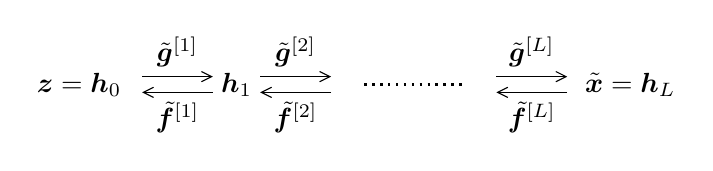
\begin{tikzpicture}
    \node (z) at (0,0) {};
    \node at ($(z)-(0.5,0)$){$\bm{z}=\bm{h}_0$};
    \node (xi1) at (1.5,0) {$\bm{h}_1$};
    \node (xi2) at (3,0) {};
    \node (xi3) at (4.5,0){};
    \node (x) at (6,0) {};
    \node at ($(x)+(0.5,0)$){$\tilde{\bm{x}} = \bm{h}_L$};
    \draw[->] ($(z) + (0.3,0.1)$) -- node[above]{$\tilde{\bm{g}}^{[1]}$} ($(xi1)+(-0.3,0.1)$); 
    \draw[->] ($(xi1)-(0.3,0.1)$) -- node[below]{$\tilde{\bm{f}}^{[1]}$}($(z) - (-0.3,0.1)$);
    \draw[->] ($(xi1) + (0.3,0.1)$) -- node[above]{$\tilde{\bm{g}}^{[2]}$} ($(xi2)+(-0.3,0.1)$); 
    \draw[->] ($(xi2)-(0.3,0.1)$) -- node[below]{$\tilde{\bm{f}}^{[2]}$}($(xi1) - (-0.3,0.1)$);
    \draw[->] ($(xi3) + (0.3,0.1)$) -- node[above]{$\tilde{\bm{g}}^{[L]}$} ($(x)+(-0.3,0.1)$); 
    \draw[->] ($(x)-(0.3,0.1)$) -- node[below]{$\tilde{\bm{f}}^{[L]}$}($(xi3) - (-0.3,0.1)$);
    \draw[dotted,line width = 0.3 mm] (xi2) -- (xi3);
  \end{tikzpicture}
\end{equation*}
where $\tilde{\bm{g}}^{[l]}$ and $\tilde{\bm{f}}^{[l]}$ are the $l$-th transformation in $\tilde{\bm{g}}$ and $\tilde{\bm{f}}$, respectively. In practice, $\bm{\tilde}{g}$ can be implemented by feed-forward neural networks, which we will detail later.

If every transformation in the chain of the flow is invertible, the full mapping is invertible.
Then, the probability density function relation between $p(\bm{z})$ and $p(\tilde{\bm{x}})$ follows the change of variable formula
\begin{equation}\label{chpt6:eq:change-var}
  p(\tilde{\bm{x}}) =  p(\bm{z}) \big| \mathrm{det}(\bm{J}) \big|, ~\mathrm{with}~ {\bm{z}=\tilde{\bm{f}}(\tilde{\bm{x}})},
\end{equation}
where $\mathrm{det}(\bm{J})$ denotes the determinant of Jacobian $\bm{J}$
\begin{equation}
  \bm{J} = \left[
    \begin{array}{ccc}
      \frac{\partial \tilde{f}_1}{\partial \tilde{x}_1} & \hdots & \frac{\partial \tilde{f}_1}{\partial \tilde{x}_N} \\
      \vdots & \hdots & \vdots \\
      \frac{\partial \tilde{f}_N}{\partial \tilde{x}_1} & \hdots & \frac{\partial \tilde{f}_N}{\partial \tilde{x}_N}
    \end{array}
  \right].
\end{equation}
The challenge lies in the determinant computation of the Jacobian $\bm{J}$, or equivalently, that of each transformation $\tilde{\bm{g}}^{[l]}$. \cite{DBLP:journals/corr/DinhKB14} introduced the model NICE to transform only half of the variables at a chain step, which results in triangular Jacobian of the transformation. If each transformation has a triangular Jacobian, determinant computation becomes efficient in \eqref{chpt6:eq:change-var}.
This flow architecture divides the feature $\bm{h}_l$ at the $l$'th layer into two subparts as
$\bm{h}_l = [\bm{h}_{l,a}^{\intercal} \, , \, \bm{h}_{l,b}^{\intercal}]^{\intercal}$ where
$(\cdot)^{\intercal}$ denotes transpose operation. We have the following forward and inverse relations between $(l-1)$'th and $l$'th layers:
\begin{align}\label{chpt6:eq-gl-coupling}
  \bm{h}_{l-1} &=
                 \begin{bmatrix}
                   \bm{h}_{l-1,a}\\
                   \bm{h}_{l-1,b}
                 \end{bmatrix}
  =
  \begin{bmatrix}
    \bm{h}_{l,a}\\
    \bm{m}_a(\bm{h}_{l,a})\odot \bm{h}_{l,b} + \bm{m}_b(\bm{h}_{l,a})
  \end{bmatrix},\nonumber\\
  \bm{h}_{l} &=
               \begin{bmatrix}
                 \bm{h}_{l,a}\\
                 \bm{h}_{l,b}
               \end{bmatrix}
  =
  \begin{bmatrix}
    \bm{h}_{l-1,a}\\
    \left(  \bm{h}_{l-1,b} - \bm{m}_b(\bm{h}_{l-1,a}) \right)\oslash \bm{m}_a(\bm{h}_{l-1,a}) 
  \end{bmatrix}, 
\end{align}
where $\odot$ denotes element-wise product, $\oslash$ denotes
element-wise division, and $\bm{m}_a(\cdot), \bm{m}_b(\cdot)$ can be
complex non-linear mappings (implemented by neural networks).
Then, for the flow model, the determinant of the Jacobian matrix is
\begin{equation}
  \mathrm{det}(\bm{J}) |_{\bm{z}=\tilde{\bm{f}}(\tilde{\bm{x}})} = \prod_{l=1}^L \det (\bm{J}_l) |_{\bm{h}_{l}}, ~\mathrm{with}~ \bm{h}_L = \tilde{\bm{x}},
\end{equation}
where $\bm{J}_l$ is the Jacobian of the transformation from the $l$-th layer to the $(l-1)$-th layer, i.e., the inverse transformation. We compute the determinant of the Jacobian matrix as
\begin{align}\label{eq-hl-determinate}
  \det (\bm{J}_l)|_{\bm{h}_{l}}& = \det \left[  \pd{\bm{h}_{l-1}}{\bm{h}_l} \right] \nonumber\\
                               & = \det
                                 \begin{bmatrix}
                                   \bm{I}_a & \mathbf{0} \nonumber\\
                                   \pd{\bm{h}_{l-1,b}}{\bm{h}_{l,a}} & \mathrm{diag}(\bm{m}_a(\bm{h}_{l,a}))
                                 \end{bmatrix}\nonumber\\
                               &= \det \left( \mathrm{diag}(\bm{m}_a(\bm{h}_{l,a})) \right),
\end{align}
where $\bm{I}_a$ is the identity matrix and $\mathrm{diag}(\cdot)$ returns a square matrix with the elements of $(\cdot)$ on the main diagnal. Then the probability density function of $\tilde{\bm{x}}$ is
\begin{align}
  p(\tilde{\bm{x}}) & =  p(\bm{z}) \big| \mathrm{det}(\bm{J}) \big| \nonumber\\
                    &  = p(\bm{z}) \prod_{l=1}^L \abs{\det\left( \mathrm{diag}(\bm{m}_a(\bm{h}_{l,a}))  \right)},
\end{align}
with $\bm{z}=\tilde{\bm{f}}(\tilde{\bm{x}})$.

\eqref{chpt6:eq-gl-coupling} describes a \textit{coupling} mapping between the layers. Since the coupling has a partial identity mapping, direct concatenation of multiple such coupling mappings would result in a partial identity mapping of the overall mapping $\tilde{\bm{g}}$. Therefore, techniques such as alternating the positions of the identity mapping \cite{2016arXiv160508803D} or using $1\times1$ convolution operations before each coupling mapping \cite{2018arXiv180703039K} are used to treat this issue.
Sometimes, it may not be necessary to carry all features thorough all $L$ chain steps. For instance, \cite{2016arXiv160508803D}\cite{2018arXiv180703039K} split some hidden
layer signal $\bm{h}$ and model a part of it directly as standard Gaussian to reduce computation and memory burden.

\begin{remark}
  There are alternative ways of formulating the transformation of variables. A popular one is the Inverse autoregreeesive flow (IAF) proposed in \cite{rezende2015variational}. In the IAF model, a chain step of transformation is formulated as
  \begin{equation*}
    \bm{h}_l = \bm{h}_{l-1} + \bm{u} \cdot {m}(\bm{w}^{\intercal} \bm{h}_{l-1} + b)
  \end{equation*}
  where $m$ is non-linear mapping, $\bm{w}, \bm{u}~\in \RR^{N}$ and $b\in \RR$. IAF does no use partial identity mapping as NICE. Its Jacobian is not triangular, and thus, determinant computation is more expensive. Moreover, whether it is invertible depends on the mapping $m$. The follow-up work by \cite{kingma2016IVF} created an element-wise transformation in a customized way to improve IAF such that its Jacobian and inverse are easier to compute. 
  
  In contrast to the above finite-chain flow where $L$ is a discrete finite integer, the method developed in \cite{ricky2018ODE} introduced a continuous-transformation of variables by solving an ordinary differential equation (ODE). Comparing to the discrete finite chain of transformation in normalizing flow, ODE can be viewed as a continuous chain of variable transformation. The inverse mapping and Jacobian determinant are not required in ODE method. But ODE needs to solve differentiation equations which is also challenging.
\end{remark}

\section{Generator Mixture Model and EM Training}
\label{chpt6:sec:generator-mix-em}
\begin{figure}[tp!]
  \centering
  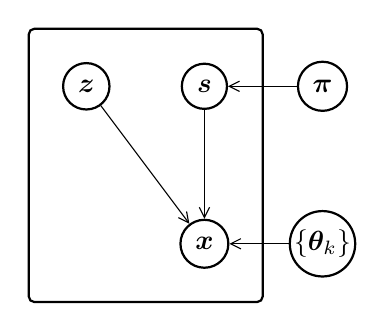
\begin{tikzpicture}
    % \tikzstyle{enode} = [thick, draw=blue, circle, inner sep = 3pt,
    % align=center]
    \tikzstyle{enode} = [thick, draw=black, circle, align=center]
    \tikzstyle{cnode} = [thick, draw=black, circle, align=center, inner sep = 0.3pt]
    
    \tikzstyle{nnode} = [thick, rectangle, rounded corners = 2pt,minimum size = 0.8cm,draw,inner sep = 12pt]
    \node[enode] (z) at (-1.5,2) {$\bm{z}$};
    \node[enode] (x) at (0,0){$\bm{x}$};
    \node[enode] (s) at (0,2){$\bm{s}$};
    \node[nnode, fit=(x)(z)(s)] (box) {};
    % \node[] at (-1.8,-0.4) {$\abs{\Dd}$};

    \node[enode] (pi) at (1.5,2){$\bm{\pi}$};
    \node[cnode] (phi) at (1.5,0){$\{ \bm{\theta}_k \}$};
    
    \draw[->] (z) to (x);
    \draw[->] (s) to (x);
    \draw[->] (pi) to (s);
    \draw[->] (phi) to (x);

  \end{tikzpicture}
  \caption{Graphical Model of GenMM.}\label{chpt6:fig:genmm-graph}
\end{figure}

\begin{figure}[tp!]
  \centering
  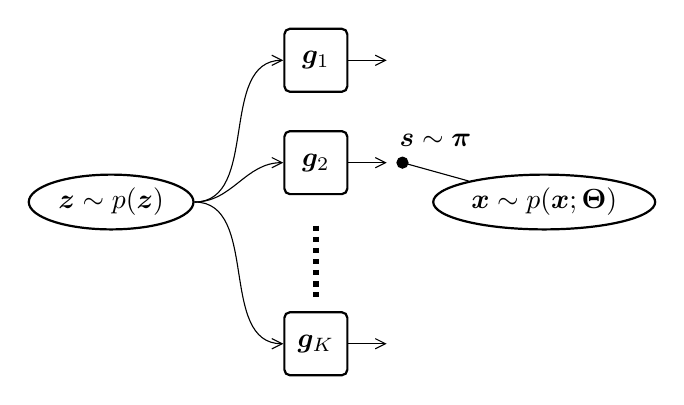
\begin{tikzpicture}
    \tikzstyle{enode} = [thick, draw=black, ellipse, inner sep = 2pt,  align=center]
    \tikzstyle{nnode} = [thick, rectangle, rounded corners = 2pt,minimum size = 0.8cm,draw,inner sep = 2pt]
    \node[enode] (z) at (0,0) {$\bm{z}\sim p(\bm{z})$};
    \node[enode] (x) at (5.5,0){$\bm{x}\sim p(\bm{x}; \bm{\Theta})$};
    % \node at (5.2,-1) {$p(\bm{x};\bm{\Phi}) = \textstyle\sum_{k=1}^K \pi_k  p_k(\bm{x})$};
    \node[nnode] (g1) at (2.6,1.8) {$\bm{g}_1$};
    \node[nnode] (g2) at (2.6,0.5) {$\bm{g}_2$};
    \node[nnode] (gk) at (2.6,-1.8) {$\bm{g}_K$};
    \draw[dotted,line width=2pt] (2.6,-0.3) -- (2.6,-1.2);
    \draw[->] (z) [in= 180, out =0] to (g1);
    \draw[->] (z) [in= 180, out =0] to (g2);
    \draw[->] (z) [in= 180, out =0] to (gk);
    \filldraw[->] (3.7, 0.5)circle (2pt) -- node[above=0.2]{$\bm{s}\sim \bm{\pi}$} (x) ;
    % \draw[->] (3,-0.8) -- (3.5, -0.8);
    \draw[->] (g1) -- (3.5,1.8);
    \draw[->] (g2) -- (3.5, 0.5);
    \draw[->] (gk) -- (3.5, -1.8);
  \end{tikzpicture}
  \caption{Signal diagram of GenMM.}\label{dia-emgm-nm}
\end{figure}

In this section, we introduce a generative model that is a mixture of $K$ flow models. All the $K$ flow models have a common input latent variable $\bm{z} \in \mathbb{R}^N$. Here, a flow $\bm{g}_k(\bm{z}): \mathbb{R}^N
\rightarrow \mathbb{R}^N$ is an instance of $\tilde{\bm{g}}$. $\bm{g}_k$ acts as the $k$-th generator and depends on a set of parameters $\bm{\theta}_k$ as
$\bm{g}_k(\bm{z})=\bm{g}(\bm{z};\boldsymbol{\theta}_k)$. We denote the induced probability density function by $\bm{g}_k$ as $p(\bm{x})|_{\bm{x}=\bm{g}_k(\bm{z})}:=p_k(\bm{x})$, i.e. $p_k(\bm{x})=p(\bm{g}_k(\bm{z}))$. For simplicity, we assume that all $K$ generators have the same chain structure. Furthermore, the distribution of $\bm{z}$ is fixed as Gaussian $\mathsf{N}(\bm{0},\bm{I})$.
The induced probability density function of $\bm{x} \in \mathbb{R}^N$ of the proposed mixture model with $K$ mixture components is given as:
\begin{align}\label{eq:FirstMixtureModel}
  p(\bm{x};\bm{\Theta})  &= \textstyle\sum_{k=1}^K \pi_k  p_k(\bm{x}) \nonumber\\
                         &= \textstyle \sum_{k=1}^K \pi_k  p(\bm{g}_k(\bm{z}))\nonumber\\
                         &= \textstyle \sum_{k=1}^K \pi_k  p(\bm{g}(\bm{z};\boldsymbol{\theta}_k)).
\end{align}
We use $\bm{\Theta}$ to denote the set of all parameters $ \{\bm{\pi},\bm{\theta}_1, \dots, \bm{\theta}_K \}$, where $\bm{\pi} = \left\{ \pi_1, \hdots, \pi_K \right\}$ is the prior distribution of the generators. Note that $\pi_k \geq 0$ and $\sum_{k=1}^K \pi_k =1$. The mixture model
in \eqref{eq:FirstMixtureModel} is called a generator mixture model (GenMM). The graphical model of GenMM is illustrated in Figure~\ref{chpt6:fig:genmm-graph}. The plate in this figure is common notation in template models (see \cite[Section~6]{koller2009pgm}), denoting that we can instantiate multiple tuple $(\bm{z}, \bm{x}, \bm{s})$ instances having dependency as illustrated. Furthermore, the
signal diagram of GenMM is illustrated in Figure~\ref{dia-emgm-nm}. The GenMM can be considered as a high-complexity model because each mixture component $p_k(\bm{x})$ has its own parameter set $\bm{\theta}_k$. 
% the parameter $\boldsymbol{\theta}_k$ varies across $K$ mixture components.

Assuming that the data in $\Dd$ is sampled i.i.d. from $p^{\ast}$, the maximum likelihood estimation problem is
\begin{equation}\label{eq:max-genmm}
  \hat{\bm{\Theta}} = \uargmax{\bm{\Theta}}{\log{\prod_{\bm{x}^{i} \in \Dd} p(\bm{x}^{i};\bm{\Theta})}},
\end{equation}
where the superscript $i$ corresponds to the $i$'th data sample in a given dataset.
We address the above maximum likelihood estimation problem using EM. 
Let us use a categorical variable $\bm{s} = [s_1, s_2, \cdots, s_K]$
for $1$-of-$K$ representation to be a hidden variable that indicates which generator is the actual one. Elements of $\bm{s}$ follow $s_k \in \{0,1\}$, $\sum_{k=1}^K s_k =1$, and $p(s_k=1)=\pi_k$. The variable $\bm{s}$ is the hidden variable in EM. We will use $\gamma_k$ to denote the posterior probability $p(s_k =1|\bm{x})$ calculated as
\begin{align}\label{eq-genmm-gamma-org}
  \gamma_k = p(s_k =1|\bm{x};\bm{\Theta}) 
  = \frac{\pi_k p(\bm{g}(\bm{z};\bm{\theta}_k))}{\sum_{l=1}^K\; \pi_l p(\bm{g}(\bm{z};\bm{\theta}_l))}.
\end{align}
Assume that a value $\bm{\Theta}^{\mathrm{old}}$ of the parameter set $\bm{\Theta}$ is given, the iterative steps in EM algorithm update $\bm{\Theta}$ as follows.
\begin{enumerate}
\item E-step: Evaluation of $\gamma_{k}^{i}$ is 
  \begin{equation}\label{eq-genmm-e-step}
    \gamma_{k}^{i}(\bm{\Theta}^{\mathrm{old}}) = \frac{\pi_k^\mathrm{{old}} p(\bm{g}(\bm{z}^{i};\bm{\theta}_k^{\mathrm{old}}))}{\sum_{l=1}^K\; \pi_l^\mathrm{{old}} p(\bm{g}(\bm{z}^{i};\bm{\theta}_l^{\mathrm{old}}))}.   
  \end{equation}
\item M-step: Evaluation of $\bm{\Theta}^{\mathrm{new}}$ given by
  \begin{equation}\label{eq-genmm-opt}
    \bm{\Theta}^{\mathrm{new}} =   \uargmax{\bm{\Theta}}{\mathcal{Q} (\bm{\Theta},\bm{\Theta}^{\mathrm{old}})}, 
  \end{equation}
  where the expected likelihood is
  \begin{equation}
    \hspace{-8pt}\mathcal{Q} (\bm{\Theta},\bm{\Theta}^{\mathrm{old}}) = \sum_{i}\sum_{k} \gamma_{k}^{i}(\bm{\Theta}^{\mathrm{old}}) \log \pi_k p_k(\bm{x}^{i}).
  \end{equation}
\end{enumerate}

For the GenMM in \eqref{eq:FirstMixtureModel}, realizing EM requires computation of $\gamma_k$ in the E-step and computation of the joint likelihood $\log{\pi_k p_k(\bm{x})}$ in the M-step. They require explicit computation of the conditional density $p_k(\bm{x}) =  p(\bm{g}_k(\bm{z})) =p(\bm{g}(\bm{z};\bm{\theta}_k))$. This is fulfilled by flow realization of generator $\bm{g}_k$. Since the chain-step transformations can be any invertible complex mapping as discussed in Section~\ref{chpt6:sec:flow}, they can be implemented by neural networks. The neural network implementation allows high flexibility of GenMM in representing complex-structured multi-modal data.

\subsection{EM Learning of GenMM}
\label{sec-algo-genmm}
The mixture model GenMM is illustrated in Figure~\ref{dia-emgm-nm},
where $K$ generators with a certain prior distribution share the same
latent distribution $p(\bm{z})$. With a neural network based flow as the generator $\bm{g}_k$ for the $k$'th mixture component in GenMM, the probability density function $p_k(\bm{x})$ for any
$\bm{x}$ can be computed exactly. Recall that $p_k(\bm{x}) =  p(\bm{g}_k(\bm{z})) =p(\bm{g}(\bm{z};\bm{\theta}_k))$ and let $\bm{f}_k$ be the inverse of $\bm{g}_k$. Then, the posterior probability can be computed further from \eqref{eq-genmm-e-step} as
\begin{align}\label{eq-genmm-gamma}
  \gamma_k({\bm{\Theta}}^{\mathrm{old}}) = \frac{\pi_k^{\mathrm{old}} p(\bm{f}_k(\bm{x})) \big|\det\left( \pd{\bm{f}_k(\bm{x})}{\bm{x}} \right)\big|}{\sum_{j=1}^K\; \pi_j^{\mathrm{old}} p(\bm{f}_j(\bm{x})) \big|\det\left( \pd{\bm{f}_j(\bm{x})}{\bm{x}} \right)\big|},
\end{align}
and the objective function in the M-step can be written as
\begin{align}\label{eq-genmm-obj}
  &\Qq\left(\bm{\Theta},\bm{\Theta}^{\mathrm{old}}\right)  \nonumber\\
  =&\sum_{i=1}^{\abs{\Dd}} \sum_{k=1}^{K}\gamma_k^{(i)}(\bm{\Theta}^{\mathrm{old}})\bigg[ \log\;\pi_k +\log\;p(\bm{f}_k(\bm{x}^{(i)})) + \log\;\bigg|\det\left(\pd{\bm{f}_k(\bm{x}^{(i)})}{\bm{x}^{(i)}} \right)\bigg|\bigg].
\end{align}
We usually deal with a large dataset for model learning, i.e. $\abs{\Dd}$ can be large. In that case we implement the EM algorithm in batch fashion. 
Recall that $ \bm{\Theta}= \{\bm{\pi},\bm{\theta}_1, \dots, \bm{\theta}_K \}$ and hence the M-step optimization problem $\argmax_{\bm{\Theta}} \mathcal{Q} (\bm{\Theta},\bm{\Theta}^{\mathrm{old}})$ is addressed in two steps:
\begin{itemize}
\item[(a)] optimizing with regard to $\{ \bm{\theta}_k \}_{k=1}^{K}$,
\item[(b)] optimizing with regard to $\bm{\pi}$.
\end{itemize}

\begin{algorithm}[!t]
  \caption{EM for learning GenMM}\label{flow-algo-em}
  \begin{algorithmic}[1]
    \STATE {\bfseries Input:}
    Latent distribution: $p(\bm{z})$. Empirical distribution $P_d(\bm{x})$ of the input dataset;
    \STATE Set a total number of epochs $T$ for training, a prior distribution $\bm{\pi}$, EM update gap $t_{\mathrm{EM}}$;
    \STATE  Set a learning rate $\eta$. 
    \STATE Build two models with parameter sets:
    \STATE ${\bm{\Theta}}^{\mathrm{old}}=\{ \bm{\pi}^{\mathrm{old}},
    \bm{\th}_1^{\mathrm{old}},\hdots,
    \bm{\th}_K^{\mathrm{old}} \}$,
    \STATE ${\bm{\Theta}} = \{ \bm{\pi},
    \bm{\th}_1,\hdots, \bm{\th}_K \}$.
    \STATE Initialize the generator prior distribution $\pi_k = 1/K$;\\ Initialize $\bm{\theta}_k$ of $\bm{g}_k$, for all $k=1,\dots,K$ randomly. 
    \STATE $\bm{\Theta}^{\mathrm{old}} \gets \bm{\Theta}$.
    \FOR { {epoch} $t < T$}
    \FOR{the iteration in epoch $t$} %\Comment{M-Step}
    \STATE Sample a batch of data $\left\{ \bm{x}^{(i)}
    \right\}_{i=1}^{n_b}$ from the dataset $\Dd$ 
    \STATE Compute $\gamma_k^{i}(\bm{\Theta}^{\mathrm{old}})$ as in \eqref{eq-genmm-gamma},
    for all $\bm{x}^{i}$ and $k=1, \dots, K$
    % \Comment{Calculate posterior \autoref{eq-posterior-gamma}}
    \STATE Compute
    $\Qq\left(\bm{\Theta},\bm{\Theta}^{\mathrm{old}}\right)$ as in \eqref{eq-genmm-obj}%\Comment{Expectation}
    
    \STATE $\partial{g_k} \gets \nabla_{\bm{\th}_k} \frac{1}{n^{b}}\Qq\left(
      \bm{\Theta}, \bm{\Theta}^{\mathrm{old}}\right)$,
    $\forall \bm{\th}_k \in \bm{\Theta}$
    \STATE $\bm{\th}_k \gets \bm{\th}_k + \eta \cdot \partial{g_k}$, $\forall \bm{\th}_k \in \bm{\Theta}$
    \ENDFOR
    % \STATE $\th_k^{t+1} \gets \th_k$, $\forall k$ %\Comment{Update new
    % parameters}
    \IF{$(t \mod t_{\mathrm{EM}} ) = 0$}
    \STATE $\pi_k \gets \EE_{\Dd}\left[ \gamma_k \right]$ %\Comment{Update perior}
    \STATE $\bm{\Theta}^{\mathrm{old}} \gets \bm{\Theta}$.
    \ENDIF
    \ENDFOR
  \end{algorithmic}
\end{algorithm}


Finding a closed-form solution for the problem $\argmax{\{\bm{\theta}_k\}_{k=1}^{K}}{ \mathcal{Q} (\bm{\Theta},\bm{\Theta}^{\mathrm{old}})}$ is not feasible in general. Instead, we use the batch-size gradient decent to optimize with regard to $\{\bm{\theta}_k\}_{k=1}^{K}$.
Further, optimization in the batch fashion leads to a practical problem as follows. 
Since $\bm{\theta}_k$ is the parameter set of the neural networks $\bm{g}_k$, one update step of gradient decent would update the generator $\bm{g}_k$ and we would lose the old mixture model parameter set $\bm{\Theta}^{\mathrm{old}}$ that is needed to compute the posteriors $\gamma_k(\bm{\Theta}^{\mathrm{old}})$ and to update $\bm{\pi}$. Thus, in learning GenMM, we maintain two such models with parameter sets $\bm{\Theta}$ and $\bm{\Theta}^{\mathrm{old}}$. At the beginning of an EM step, $\bm{\Theta} = \bm{\Theta}^{\mathrm{old}}$. While we optimize $\{\bm{\theta}_k\}_{k=1}^{K}$ of $\bm{\Theta}$ with batch-size gradient decent, we use the model with old parameter set $\bm{\Theta}^{\mathrm{old}}$ to do posterior computation and update of $\bm{\pi}$. At the end of the EM step, the old parameter set is replaced by the updated one: $\bm{\Theta}^{\mathrm{old}}\gets \bm{\Theta}$.



Next, we discuss the optimization of the prior distribution $\bm{\pi}$. The optimization problem is 
\begin{equation}\label{eq-pi-update1}
  \bm{\pi}^{\mathrm{new}} = \uargmax{\bm{\pi}}{ \mathcal{Q}
    (\bm{\Theta},\bm{\Theta}^{\mathrm{old}})}, \,\,
  \mathrm{s.t.} \sum_{k=1}^{K}\pi_k = 1.
\end{equation}
The update of prior follows the solution
\begin{equation}\label{eq-pi-solution}
  \pi_k^{\mathrm{new}} = \frac{1}{\abs{\Dd}}\sum_{i=1}^{\abs{\Dd}}\gamma_k^{i}(\bm{\Theta}^{\mathrm{old}}).
\end{equation}
The detail to get the solution is derived in the Section~\ref{subsubsec:Proof_for_update}. For a given dataset with empirical distribution $P_d(\bm{x})$,
$\gamma_k$ is evaluated with batch data in order to calculate the cost
$\Qq\left(\bm{\Theta},\bm{\Theta}^{\mathrm{old}}\right)$ and to update the
parameter $\bm{\theta}_k$ of $\bm{g}_k$. We accumulate the values of $\gamma_k$ of batches and
average out for one epoch to update $\bm{\pi}$, {i.e.}, $\pi_k \gets \EE_{\Dd}\left[ \gamma_k \right]$.



We summarize the EM algorithm for GenMM in Algorithm~\ref{flow-algo-em}.
In implementation, to avoid numerical computation problem, $\log{p(\bm{g}(\bm{z}; \bm{\theta}_k))}$ is
scaled by the dimension of signal $\bm{x}$ in order to compute $\gamma_k$. 

\subsection{Detailed Derivation of the Update for $\pi$}
\label{subsubsec:Proof_for_update}

The optimization of $\bm{\pi}$ is addressed in the following Lagrangian form
\begin{equation}
  \Ff(\bm{\Theta}) = \mathcal{Q}(\bm{\Theta},\bm{\Theta}^{\mathrm{old}}) + \lambda
  \left( 1 - \sum_{k=1}^{K}\pi_k \right),
\end{equation}
where $\lambda$ is the Lagrange multiplier. Then
\begin{align}
  \bm{\pi}^{\mathrm{new}} =& \uargmax{\bm{\pi}}{ \Ff(\bm{\Theta})} \nonumber\\
  =&  \uargmax{\bm{\pi}}{}\sum_{i=1}^{\abs{\Dd}}
     \sum_{k=1}^{K}\gamma_k^{i}(\bm{\Theta}^{\mathrm{old}})\bigg[
     \log\;\pi_k +   \log\;p(\bm{f}_k(\bm{x}^{i})) \nonumber \\
                           &+ \log\;\bigg|\det\left(
                             \pd{\bm{f}_k(\bm{x}^{i})}{\bm{x}^{i}}
                             \right)\bigg|\bigg] + \lambda  \left( 1 - \sum_{k=1}^{K}\pi_k \right) \nonumber\\
  =& \uargmax{\bm{\pi}}{} \sum_{i=1}^{\Dd}
     \sum_{k=1}^{K}\gamma_k^{i}(\bm{\Theta}^{\mathrm{old}})
     \log\;\pi_k+ \lambda  \left( 1 - \sum_{k=1}^{K}\pi_k \right),
\end{align}
where $\bm{f}_k = \bm{g}_k^{-1}$. Then solving
\begin{equation}
  \pd{\Ff}{\pi_k} = 0, k=1, 2, \cdots, K,
\end{equation}
we get 
$
\pi_k = \frac{1}{\lambda}
\sum_{i=1}^{n}\gamma_k^{i}(\bm{\Theta}^{\mathrm{old}}), \forall k.
$
With the condition $\sum_{k=1}^{K}\pi_k =1$, we have
$
\lambda = \sum_{k=1}^{K}\sum_{i=1}^{\abs{\Dd}}\gamma_k^{i}(\bm{\Theta}^{\mathrm{old}}) =\abs{\Dd}.
$
Therefore, the solution is
$
\pi_k = \frac{1}{\abs{\Dd}}
\sum_{i=1}^{\abs{\Dd}}\gamma_k^{i}(\bm{\Theta}^{\mathrm{old}}), \forall k.
$
Note that the updated prior parameter $\pi_k$
is non-negative due to the non-negativity of the posterior $\gamma_k^{i}$.

\subsection{On the Convergence of GenMM}
Now we analysis the convergence behaviour of GenMM. Under the conditions that we present as follows, GenMM converges. 

\begin{proposition}
  Assume that for all $k$, the parameters $\bm{\theta}_k$ are in a compact set such that the corresponding mapping $\bm{g}_k$ is invertible. Assume further that all generator mappings fulfill that $\bm{f}_k$ and $\frac{\partial \bm{f}_k}{\partial \bm{x}}$ are continuous functions of $\bm{\theta}_k$. Then GenMM converges. 
  % Suppose that all the generator mappings $\bm{g}_k$ are such that $\bm{f}_k$ and $\frac{\partial \bm{f}_k}{\partial \bm{x}}$ are continuous functions of $\bm{\theta}_k$. Assume further that for all $k$, the parameters $\bm{\theta}_k$ are in a compact set such that the corresponding mapping $\bm{g}_k$ is invertible. Then GenMM converges. 
  % \textcolor{red}{Do you think it is possible to say: The GenMM converges to a saddle point. In that case the confusion about usual understanding on convergence to local minima does not arise.}
\end{proposition}
\begin{proof}
  Assume that the assumption holds. Then the determinant term $\det(\bm{J})$ in \eqref{chpt6:eq:change-var} is a continuous function of $\bm{\theta}_k$. Due to \eqref{chpt6:eq:change-var} and the continuity of Gaussian density $p(\bm{z})$, the probability density function $p_k(\bm{x})$ is a continuous function of $\bm{\theta}_k$. Therefore, $p(\bm{x})$ given in \eqref{eq:FirstMixtureModel} is a continuous function of $\bm{\Theta}$. Denote the likelihood in \eqref{eq:max-genmm} as $\Ll(\bm{\Theta})=\log \textstyle\prod_{i} p(\bm{x}^{(i)};\bm{\Theta})$. The maximum value of $\Ll(\bm{\Theta})$ is bounded due to continuity of $p(\bm{x})$ with regard to $\bm{\Theta}$.
  Define $\hat{F}(\bm{\Theta}) = \Qq\left(\bm{\Theta},\bm{\Theta}^{\mathrm{old}}\right) - \sum_{i=1}^{\abs{\Dd}}\sum_{k=1}^{K}\gamma_k^{i}(\bm{\Theta}^{\mathrm{old}}) \log\gamma_k^{(i)}(\bm{\Theta}^{\mathrm{old}})$ (note $\hat{F}$ is the empirical version of lower bound in \eqref{chpt5:eq:lower-bound-F}). It is well known that $\hat{F}(\bm{\Theta})$ is a lower bound on the likelihood function $\Ll(\bm{\Theta})$, i.e. $\Ll(\bm{\Theta}) \geq \hat{F}(\bm{\Theta})$.

  Note that the essence of EM algorithm is that the likelihood function value is elevated by increasing the value of its lower bound $\hat{F}(\bm{\Theta})$. Since the maximum value of the log-likelihood $\Ll(\bm{\Theta})$ is finite, $\hat{F}(\bm{\Theta})$ can not grow unbounded.
  % Actually the maximization of $\Ll(\bm{\Phi})$ solved by EM is done by keeping increasing a lower bound of likelihood $\Ll(\bm{\Phi})$: 
  % .
  % The inequality  always holds.
  % $\mathcal{Q}(\cdot,\bm{\Phi}^{\mathrm{old}})$ can not grow unbounded, i.e., the EM converges under the %assumption as $\mathcal{Q}(\bm{\Phi}^{\mathrm{new}},\bm{\Phi}^{\mathrm{new}})\geq %\mathcal{Q}(\bm{\Phi}^{\mathrm{old}},\bm{\Phi}^{\mathrm{old}})$ after each iteration.

  % \textcolor{red}{Therefore an important issue is that the log-likelihood is finite. But, is there any chance that it can not hold? Means somehow it goes unbounded. What is the condition that likelihhod function is guaranteed to be finite with its parameters?}
\end{proof}


\section{A low-complexity model}
There are $K$ flow generators implemented as neural networks in GenMM, which makes GenMM a high-complexity model.
We now propose a low-complexity model where parameters are shared. This is motivated by many machine learning setups where model parameters are shared across model components. For example, this technique is applied as the use of shared covariance matrices in a tied Gaussian mixture model, in linear discriminant analysis \cite{bellegarda1990tiedmixture, Kimball:1993:UTD:1075671.1075694, Bishop:2006:PRM:1162264}, and the use of a common subspace in non-negative matrix factorization \cite{Gupta2013}. Based on the idea of sharing parameters, we propose a low-complexity model which we refer to as a latent mixture model as follows.

\subsection{Latent mixture model}\label{subsec-latmm}

In this generative model, we use a latent variable $\bm{z}$ that has the following Gaussian mixture distribution
\begin{equation}
  p(\bm{z}) = \sum_{k=1}^K \pi_k p_k(\bm{z}), % = \sum_{k=1}^K \pi_k \mathcal{N}(\bm{z};\bm{\mu}_k,\bm{C}_k),
\end{equation}
where $p_k(\bm{z})$ is probability density function of a Gaussian distribution $\mathsf{N}(\bm{z};\bm{\mu}_k,\bm{C}_k)$ with mean $\bm{\mu}_k$ and covariance $\bm{C}_k$.
The data $\bm{x}$ is
assumed to be generated in the model using a single neural network
$\bm{g}(\bm{z}): \mathbb{R}^N \rightarrow \mathbb{R}^N$ as
$\bm{x}=\bm{g}(\bm{z};\bm{\theta})$, where $\bm{\theta}$
is the set of parameters of the neural network. The diagram of this mixture model
is shown in Figure~\ref{dia-emgm-sm}. Similarly, we use $\ubar{\bm{\Theta}}$ to denote the set of all parameters $\{ \bm{\pi},
\bm{\mu}_1,\hdots, \bm{\mu}_K, \bm{C}_1,\hdots,
\bm{C}_K, \bm{\theta} \}$. Furthermore, we also have a categorical variable $\bm{s}$ to indicate which underlying source is chosen. The density function of the proposed latent mixture model (LatMM) is given as
\begin{align}\label{eq:SecondMixtureModel}
  p(\bm{x};\ubar{\bm{\Theta}}) & = \textstyle\sum_{k=1}^K \pi_k p_k(\bm{x}) \nonumber\\
                               &= \textstyle\sum_{k=1}^K \pi_k  p(\bm{g}(\bm{z}; \bm{\theta})| s_k=1) \nonumber \\
                               & = \textstyle\sum_{k=1}^K \pi_k  p(\bm{g}(\bm{z};\bm{\theta}); \bm{\mu}_k, \bm{C}_k).
\end{align}
The LatMM is illustrated in Figure~\ref{dia-emgm-sm} where the neural network $\bm{g}$ is shared. Learning of LatMM requires solving the maximum likelihood estimation problem
\begin{equation}
  \ubar{\hat{\bm{\Theta}}} =    \uargmax{\ubar{\bm{\Theta}}}{} \log \prod_{i} p(\bm{x}^{(i)};\ubar{\bm{\Theta}}),
\end{equation}
which we address using EM.
We have
\begin{align}\label{eq-latMM-gamma}
  \ubar{\gamma}_k = p(s_k =1|\bm{x};\ubar{\bm{\Theta}})  
  = \frac{\pi_k p(\bm{g}(\bm{z};\bm{\theta});\bm{\mu}_k, \bm{C}_k)}{\sum_{l=1}^K\; \pi_l p(\bm{g}(\bm{z};\bm{\theta});\bm{\mu}_l, \bm{C}_l)}.
\end{align}

Similar to the case of GenMM, realization of the corresponding EM
algorithm associated with LatMM in Figure~\ref{eq:SecondMixtureModel}
also requires computing the posterior distribution $\ubar{\gamma}_k$ and the joint likelihood $\log{\pi_k p_k(\bm{x})}$. They require explicit computation of the conditional density function $p_k(\bm{x}) = p(\bm{g}(\bm{z};\bm{\theta})| s_k=1) = p(\bm{g}(\bm{z};\bm{\theta});\bm{\mu}_k, \bm{C}_k) $. In LatMM, $\bm{g}(\bm{z}): \mathbb{R}^N \rightarrow \mathbb{R}^N$ is also required to be invertible. Again $\bm{g}$ is instantiated from flow $\tilde{\bm{g}}$ in Section~\ref{chpt6:sec:flow}. Then, the problem is how to learn the parameters of LatMM.

\begin{figure}
  \centering
  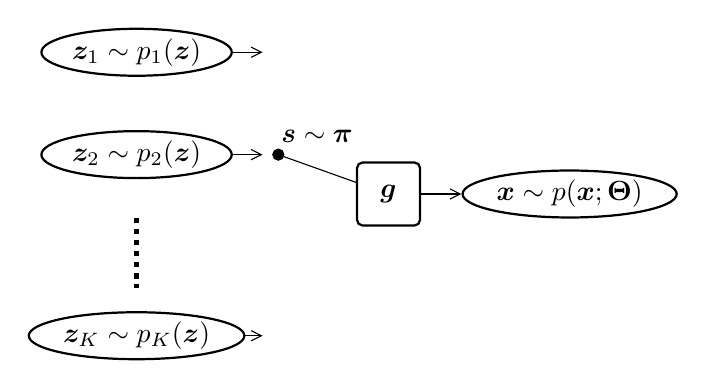
\begin{tikzpicture}
    \tikzstyle{enode} = [thick, draw=black, ellipse, inner sep = 1pt,  align=center]
    % \tikzstyle{nnode} = [thick, rectangle, rounded corners = 1pt,minimum size = 1.2cm,draw,inner sep = 2pt]
    \tikzstyle{nnode} = [thick, rectangle, rounded corners = 2pt,minimum size = 0.8cm,draw,inner sep = 2pt]
    \node[enode] (z1) at (0,1.8) {$\bm{z}_1\sim p_1(\bm{z})$};
    \node[enode] (z2) at (0,0.5){$\bm{z}_2\sim p_{2}(\bm{z})$};
    \node[enode] (zK) at (0,-1.8) {$\bm{z}_K\sim p_{K}(\bm{z})$}; 
    \node[enode] (x) at (5.5,0){$\bm{x}\sim p(\bm{x};\ubar{\bm{\Theta}})$};
    % \node at (3,-1){$p(\bm{z}) = \sum_k\pi_kp_k(\bm{z})$};
    \node[nnode] (g) at (3.2,0) {$\bm{g}$};
    \draw[dotted,line width=2pt] (0,-0.3) -- (0,-1.2);
    \filldraw[->] (1.8, 0.5)circle (2pt) -- node[above=0.2]{$\bm{s}\sim \bm{\pi}$} (g) ;
    \draw[->] (z1) -- (1.6, 1.8);
    \draw[->] (z2) -- (1.6, 0.5);
    % \draw[->] (1,-0.5) -- (1.8, -0.5);
    \draw[->] (zK) -- (1.6, -1.8);
    % \draw[->] (z1) [in=180,out=0]  to node[right]{$\pi_1$} (g);
    % \draw[->] (z2) [in=180,out=0]  to node[above]{$\pi_2$} (g);
    % \draw[->,dashed] (zK) [in=180,out=0]  to node[right]{$\pi_K$} (g);
    \draw[->] (g) to (x);
  \end{tikzpicture}
  \caption{Diagram of LatMM.}\label{dia-emgm-sm}
\end{figure}


\subsection{EM Algorithm for LatMM}
\begin{algorithm}[t]
  \caption{EM for learning LatMM}\label{flow-algo-sem}
  \begin{algorithmic}[1]
    \STATE {\bfseries Input:} Empirical distribution $P_d(\bm{x})$ of dataset;
    \STATE Latent mixture distribution: 
    \STATE $\sum_{k=1}^{K}\pi_k \Nn\left(\bm{z}; \bm{\mu}_k, \mathrm{diag}(\bm{\sigma}_k^2)\right)$
    \STATE Set a total number of epochs $T$ of training, prior $\bm{\pi}$ update gap $t_{\pi}$, EM update gap $t_{\mathrm{EM}}$, a learning rate $\eta$; Set hyperparameter $a$ , $b$ for prior of
    $\bm{\sigma}_k^{-1}, \forall k$.
    \STATE Build two models with parameter sets:
    \STATE $\ubar{\bm{\Theta}}^{\mathrm{old}}=\{ \bm{\pi}^{\mathrm{old}},
    \bm{\mu}_1^{\mathrm{old}},\hdots, \bm{\mu}_K^{\mathrm{old}}, \bm{\sigma}_1^{\mathrm{old}},\hdots,
    \bm{\sigma}_K^{\mathrm{old}}, \bm{\theta}^{\mathrm{old}} \}$,
    \STATE $\ubar{\bm{\Theta}} = \{ \bm{\pi},
    \bm{\mu}_1,\hdots, \bm{\mu}_K, \bm{\sigma}_1,\hdots,
    \bm{\sigma}_K, \bm{\theta} \}$.
    \STATE Initialize the generator prior distribution $\pi_k = 1/K$ and initialize its $\bm{\theta}$ for $\bm{g}$, $\bm{\mu}_k$, $\bm{\sigma}_k$, $\forall k$ randomly.
    \STATE $\ubar{\bm{\Theta}}^{\mathrm{old}} \gets \ubar{\bm{\Theta}}$
    % \STATE 
    \FOR {epoch $t < T$}
    \FOR{the iteration in epoch $t$}
    \STATE Sample a batch of data $\left\{ \bm{x}^{(i)}
    \right\}_{i=1}^{n_b}$ from dataset
    \STATE Compute $\ubar{\gamma}_k(\ubar{\bm{\Theta}}^{\mathrm{old}})$ by \ref{em-latmm-gamma}, $\forall \bm{x}^{(i)}$ and $k=1, 2, \cdots, K$ %= \frac{\pi_k \Nn\left(f(X); \bm{\mu}_k^{t},\bm{\sigma}_k^{t}\right)}{\sum_{k=1}^K\; \pi_k\Nn\left(f(X); \bm{\mu}_k^{t},\bm{\sigma}_k^{t}\right) }, \forall \left\{ x^{(i)}\right\}_{i=1}^{n_b}$
    % \Comment{Calculate posterior \autoref{eq-posterior-gamma}}
    \STATE Compute
    $\ubar{\Qq}\left(\ubar{\bm{\Theta}},\ubar{\bm{\Theta}}^{\mathrm{old}}\right)$ by \ref{eq-latmm-obj}%\Comment{Expectation}

    \STATE $\partial{\bm{\th}}, \partial{\bm{\mu}_k}, \partial{\bm{\sigma}_k}\gets 
    \nabla_{\bm{\theta}, \bm{\mu}_k, \bm{\sigma}_k} 
    \frac{1}{n^{b}}\ubar{\Qq}\left(\ubar{\bm{\Theta}},\ubar{\bm{\Theta}}^{\mathrm{old}}\right)
    +\frac{1}{K}
    \log\prod_{k=1}^K
    \Gamma(\bm{\sigma}_k^{-1};
    a, b)$ %\Comment{E-step}
    % \STATE $\partial{g_k} \gets \nabla_{\th_k}\widetilde{\Qq}\left(\left\{ \th_k
    %   \right\}_{k=1}^{K};\left\{ \th_k^t\right\}_{k=1}^{K}\right)$,
    % $\forall \th_k \in\left\{ \th_k\right\}_{k=1}^{K}$
    \STATE $\bm{\th} \gets \bm{\th} + \eta \cdot \partial{\bm{\theta}}$
    \STATE $\bm{\mu}_k \gets \bm{\mu}_k + \eta \cdot \partial{\bm{\mu}_k}, \forall k$
    \STATE $\bm{\sigma}_k \gets \bm{\sigma}_k + \eta \cdot \partial{\bm{\sigma}_k},
    \forall k$
    \ENDFOR
    % \IF{$(t \mod t_{\pi} )=0$} %\Comment{M-Step}

    % \ENDIF
    \IF{$(t \mod t_{\mathrm{EM}} )=0$} %\Comment{M-Step}
    \STATE $\pi_k \gets \EE_{P_d}\left[ \ubar{\gamma}_k(\ubar{\bm{\Theta}}^{\mathrm{old}}) \right]$%\Comment{Update perior}
    \STATE $\ubar{\bm{\Theta}}^{\mathrm{old}} \gets \ubar{\bm{\Theta}}$
    \ENDIF
    \ENDFOR
  \end{algorithmic}
  % \hspace{0.5cm}
\end{algorithm}


Algorithm~\ref{flow-algo-sem} summarizes the EM algorithm for LatMM.
LatMM is used to
learn one generative model that gets input from a mixture latent source
distribution with one single generator $\bm{g}$. For simplicity, we set
the covariance matrix of each latent Gaussian source as a diagonal
matrix, $\bm{C}_k = \mathrm{diag}(\bm{\sigma}_k^2) $. Each component $p_k(\bm{z})$ of
the latent source $p(\bm{z})$ can be obtained by an affine transform from
the standard Gaussian, {i.e.}, $\bm{z}_k \sim p_k(\bm{z})$ can be
obtained by a linear layer of neural network with $\bm{z}_k = \bm{\mu}_k
+ \bm{\sigma}_k \bm{\epsilon}, \bm{\epsilon} \sim \mathsf{N}(\bm{0}, \bm{I})$.
According to Section~\ref{subsec-latmm}, the posterior and objective function in M-step of LatMM can be respectively computed as
\begin{align}\label{em-latmm-gamma}
  \ubar{\gamma}_k(\ubar{\bm{\Theta}}^{\mathrm{old}}) = \frac{\pi_k^{\mathrm{old}} p_k\left(\bm{z}\right)}{\sum_{j=1}^K\;\pi_j^{\mathrm{old}} p_j\left(\bm{z}\right)}\bigg|_{\bm{z}=\bm{f}(\bm{x})},
\end{align}
\begin{align}\label{eq-latmm-obj}
  &\ubar{\Qq}\left( \ubar{\bm{\Theta}},\ubar{\bm{\Theta}}^{\mathrm{old}}\right) \nonumber \\
    =&\sum_{i=1}^n \log\;\bigg|\det\left(
    \pd{\bm{f}(\bm{x}^{(i)})}{\bm{x}^{(i)}} \right)\bigg| 
  + \sum_{k=1}^{K}\ubar{\gamma}_k^{(i)}(\ubar{\bm{\Theta}}^{\mathrm{old}})\bigg[ \log{\pi_k}
    +\log{p_k\left(\bm{f}(\bm{x}^{(i)}); \bm{\mu}_k, \bm{\sigma}_k^2\right)}\bigg], 
\end{align}
where $\bm{f}$ is the inverse of $\bm{g}$.
Similar to Section~\ref{sec-algo-genmm}, update of prior $\bm{\pi}$
follows $\pi_k \leftarrow \EE_{\Dd}[ \ubar{\gamma}_k(\bm{x})
]$. However, we need to consider the following issue when learning the parameters of
Gaussian mixture source $p(\bm{z}) = \sum_{k=1}^K \pi p_k(\bm{z})$. If a component of the mixture source overfits and collapses onto a data sample, the likelihood can be large and the parameter learning can be problematic. This problem is known as the singularity problem of Gaussian mixture \cite{Bishop:2006:PRM:1162264}.
We avoid this problem by using the following alternatives:
\begin{itemize}
\item Assume that for each $\forall k=1, 2, \cdots, K$, there is a parameter prior distribution for $\bm{C}_k=\mathrm{diag}(\bm{\sigma}_k^2)$.
  To be specific, assume that the parameter prior distribution of the precision $\bm{\sigma}_k^{-1}$ is
  $\Gamma(\bm{\sigma}_k^{-1};a, b)$, where $\Gamma(\cdot; a, b)$ is
  Gamma distribution with parameter $a$ and $b$. Then, the objective function of the optimization problem with regard to $\bm{\Theta}$ is reformulated as
  \begin{equation}\label{eq-latmm-obj1}
    \umax{ \ubar{\bm{\Theta}}}   \frac{1}{\abs{\Dd}}
    \ubar{\Qq}\left(\ubar{\bm{\Theta}},\ubar{\bm{\Theta}}^{\mathrm{old}} \right)
    +\frac{1}{K}
    \log\prod_{k=1}^K
    \Gamma(\bm{\sigma}_k^{-1};
    a, b).
  \end{equation}
\item Alternatively, we use an $l_2$ regularization on $\bm{\sigma}_k$,
  which formulates the optimization step as
  \begin{equation}
    \umax{\ubar{\bm{\Theta}}}   \frac{1}{\abs{\Dd}} \ubar{\Qq}\left(\ubar{\bm{\Theta}},\ubar{\bm{\Theta}}^{\mathrm{old}}\right)-\lambda \sum_{k=1}^K \frac{(1- \bm{\sigma}_k)^2}{K},
  \end{equation}
  where $\la$ is the regulation parameter.
\end{itemize}

\subsection{On complexity of models and new variant models}
We have proposed two models, GenMM and LatMM. GenMM has a high complexity whereas LatMM has low complexity. Due to their difference in model complexity as well as training complexity, their usage efficiency is highly application-dependent. For example, when the training data is limited, it may be advisable to use LatMM.

It is possible to combine GenMM and LatMM to obtain new models. A simple way is to replace the latent source $p(\bm{z})$ of GenMM by a LatMM model. 
% where latent variable $\bm{z}$ has a mixture distribution and there are multiple generators. Each generator has its own parameters. 
This new combined model has a higher complexity than both GenMM and LatMM. %The EM based training algorithm can be derived for this new model.

To get a less complex model than GenMM, another new model can be derived by modifying the architecture of LatMM. There are multiple latent sources $p_k(\bm{z})$, $k=1, 2, \cdots, K$, in LatMM. If we assume that each such latent source $p_k(\bm{z})$ is induced by a latent generator network, we can obtain a new model that has a common-and-individual architecture. Each latent generator of its corresponding latent source has its own parameters and acts as an individual part. The common part of the new model transforms signal between observable signal $\bm{x}$ and latent signal $\bm{z}$ (generated by the latent generator networks). The common-and-individual technique is prevalently used in machine learning systems\cite{sundman2016design, SUNDMAN2014298}.

Therefore several new models can be derived using our proposed models, GenMM and LatMM. In spite of the scope and potential, the development of an analytical methodology to derive new model architectures turns out to be challenging. Traditionally the development is trial-and-error driven. Development of new model architectures by combining GenMM and LatMM is not to be pursued here.   


\section{Experimental Results}\label{sec:experiments}
% \begin{figure*}[!ht]
%   \captionsetup[subfigure]{justification=centering}
%   \centering
%   \begin{subfigure}{.24\textwidth}
%     \centering
%     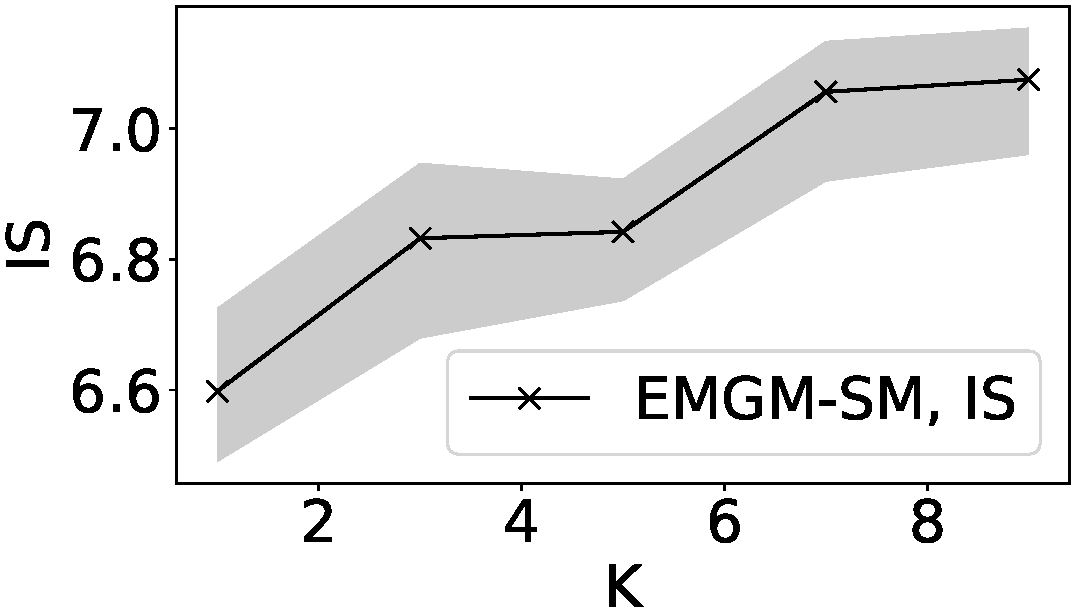
\includegraphics[width=1\linewidth]{images/mnist/scores/EMGM-NM/EMGM-NM-IS-K.pdf}
% %     \caption{IS score}
%     %     \label{fig-nm-isk}
%   \end{subfigure}
%   \vspace{-2pt}
%   \begin{subfigure}{.24\textwidth}
%     \centering
%     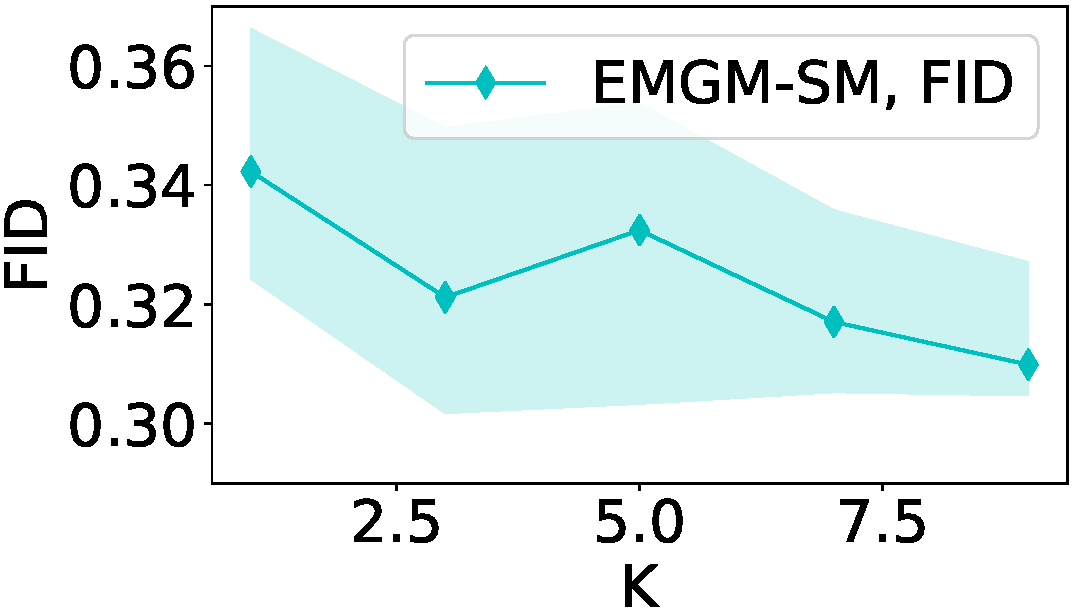
\includegraphics[width=1\linewidth]{images/mnist/scores/EMGM-NM/EMGM-NM-FID-K.pdf}
%     %     \caption{FID score}
%     %     \label{fig-nm-fidk}
%   \end{subfigure}
%   \centering
%   \begin{subfigure}{.24\textwidth}
%     \centering
%     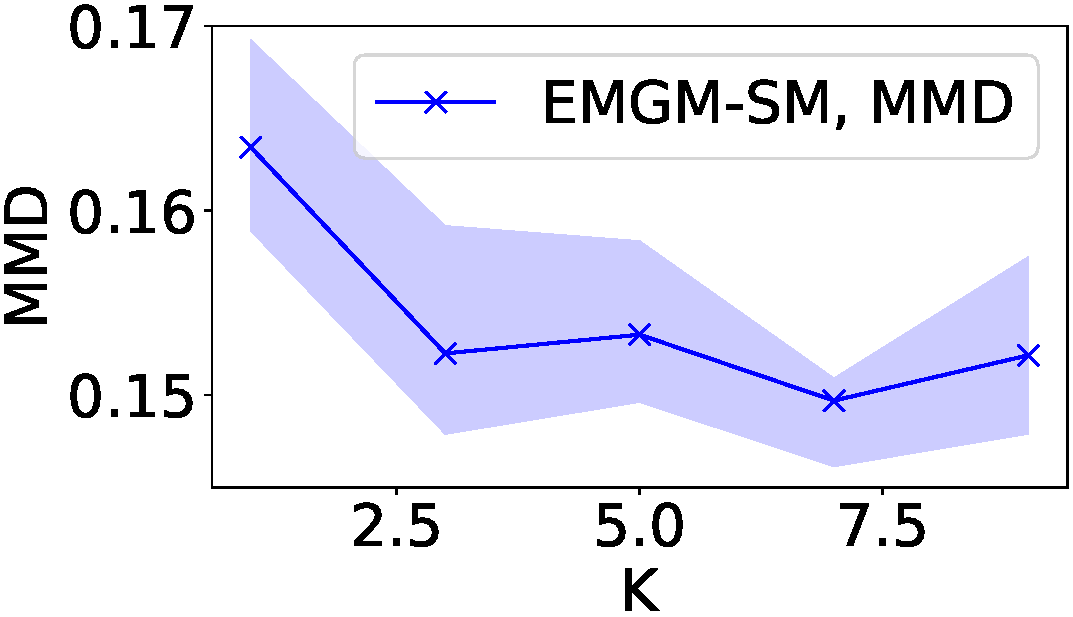
\includegraphics[width=1\linewidth]{images/mnist/scores/EMGM-NM/EMGM-NM-MMD-K.pdf}
%     %     \caption{MMD score}
%     %     \label{fig-nm-mmdk}
%   \end{subfigure}
%   \centering
%   \begin{subfigure}{0.24\textwidth}
%     \centering
%     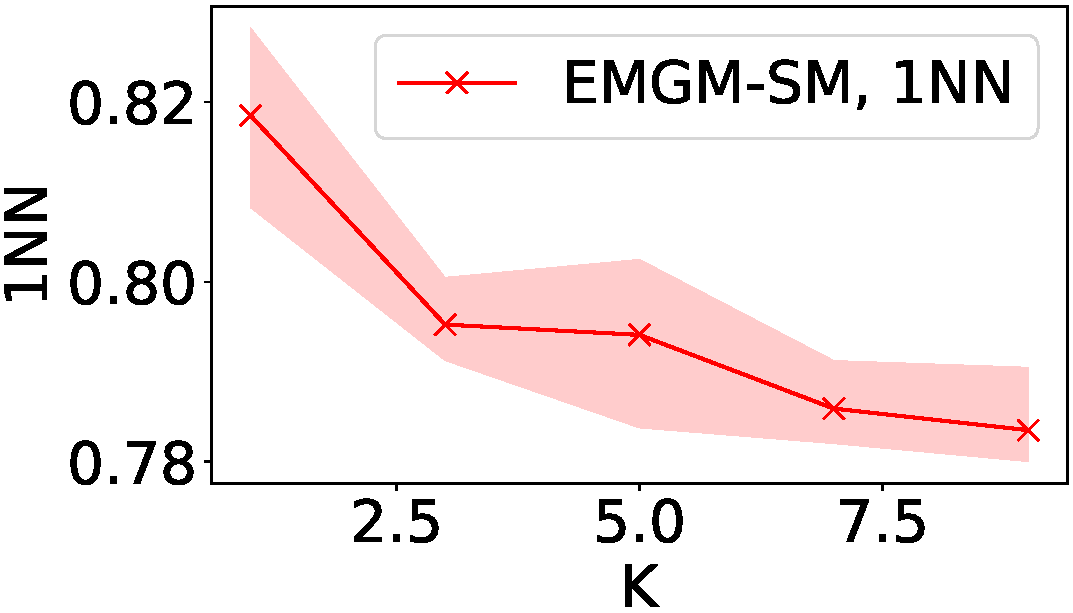
\includegraphics[width=1\linewidth]{images/mnist/scores/EMGM-NM/EMGM-NM-1NN-K.pdf}
%     %     \caption{1NN score}
%     %     \label{fig-nm-1nnk}
%   \end{subfigure}
%   \centering
%   \begin{subfigure}{.24\textwidth}
%     \centering
%     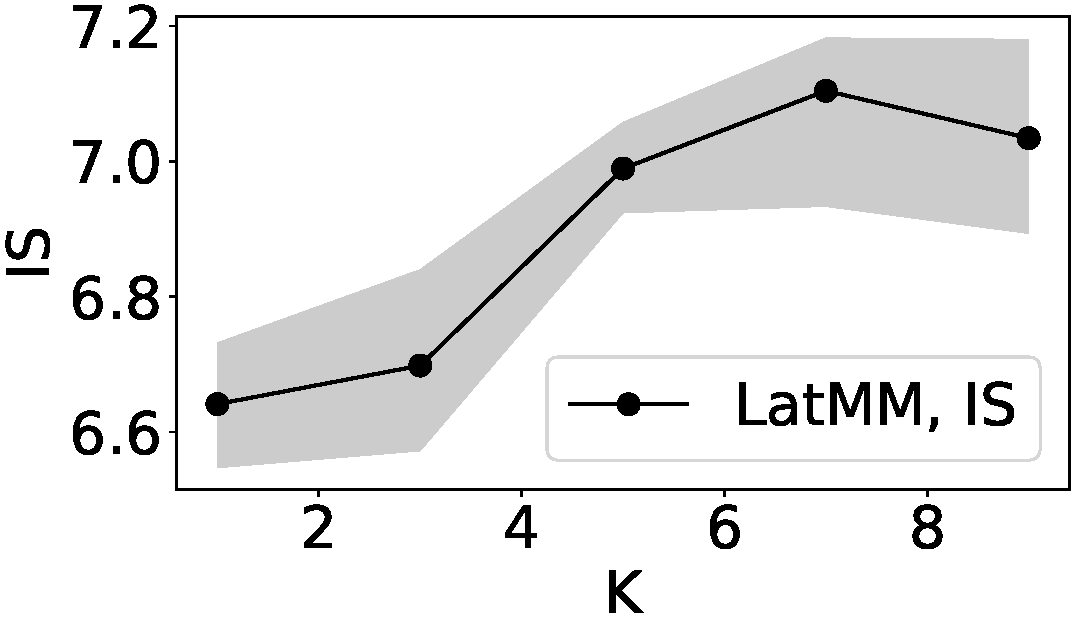
\includegraphics[width=1\linewidth]{images/mnist/scores/EMGM-SM/EMGM-SM-IS-K.pdf}
%     %     \caption{IS score}
%     %     \label{fig-sm-is}
%   \end{subfigure}
%   \centering
%   \begin{subfigure}{.24\textwidth}
%     \centering
%     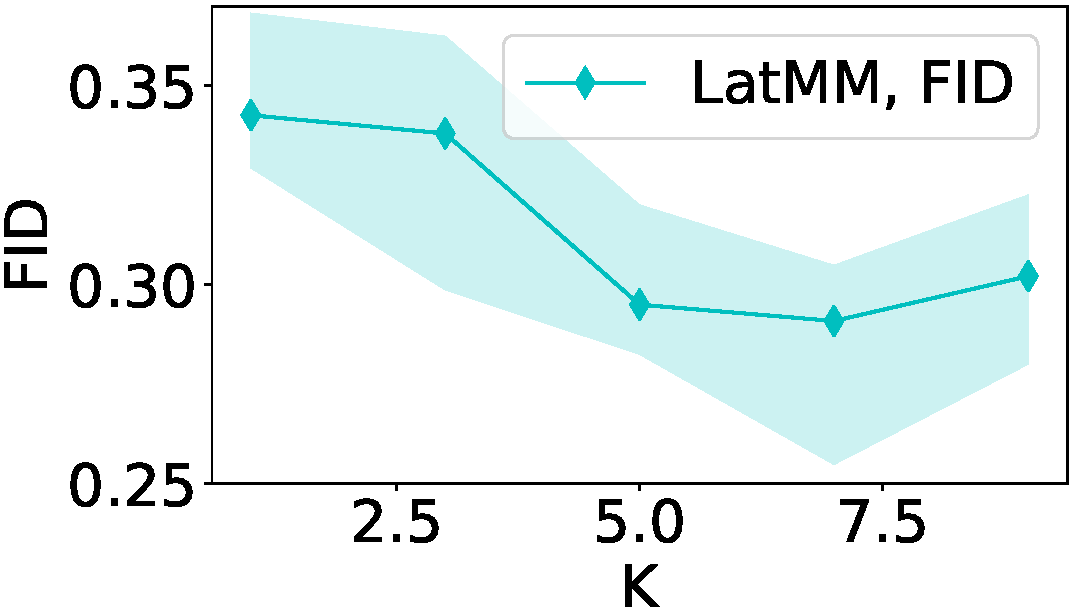
\includegraphics[width=1\linewidth]{images/mnist/scores/EMGM-SM/EMGM-SM-FID-K.pdf}
%     %     \caption{FID score}
%     %     \label{fig-sm-fid}
%   \end{subfigure}
%   \centering
%   \begin{subfigure}{.24\textwidth}
%     \centering
%     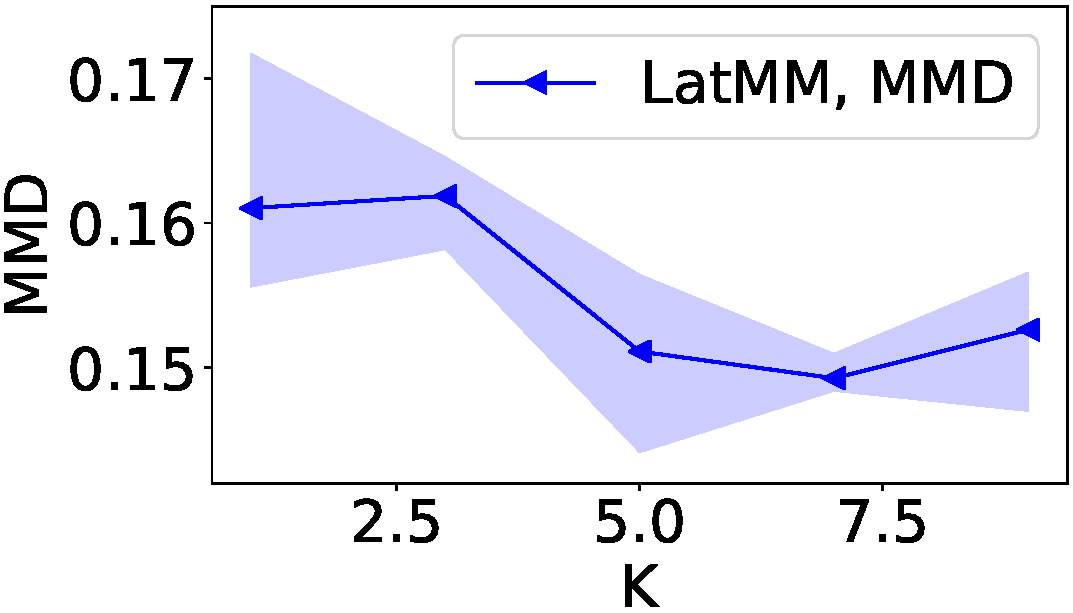
\includegraphics[width=1\linewidth]{images/mnist/scores/EMGM-SM/EMGM-SM-MMD-K.pdf}
%     %     \caption{MMD score}
%     %     \label{fig-sm-mmd}
%   \end{subfigure}
%   \begin{subfigure}{0.24\textwidth}
%     \centering
%     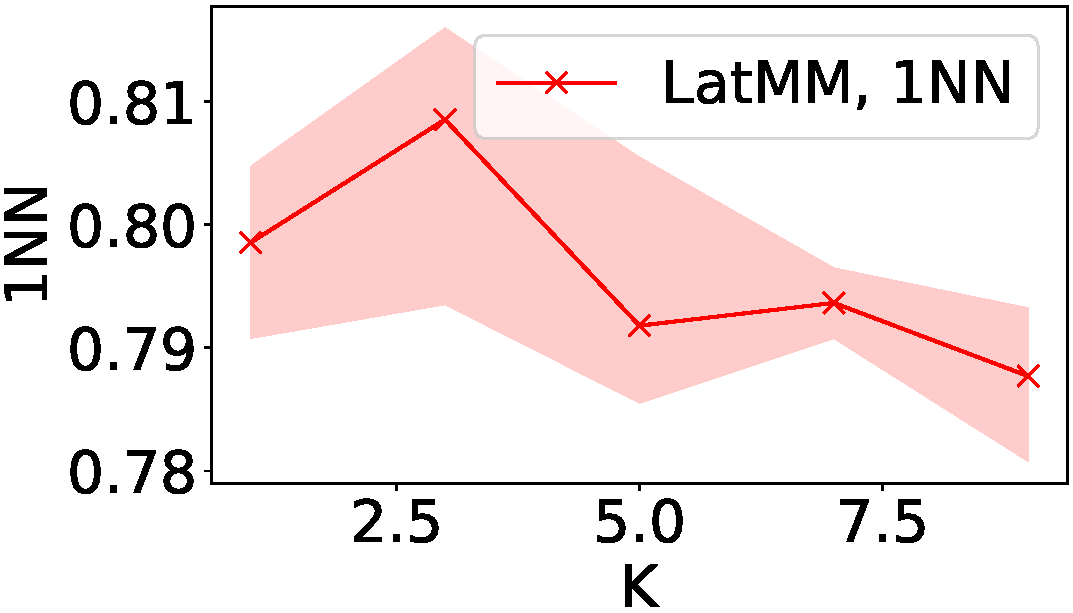
\includegraphics[width=1.\linewidth]{images/mnist/scores/EMGM-SM/EMGM-SM-1NN-K.pdf}
%     %     \caption{1NN score}
%     %     \label{fig-sm-1nn}
%   \end{subfigure}
%   \caption{IS, FID, MMD and 1NN scores of GenMM and LatMM. Evaluated
%   on $2000$ samples ($1000$ samples generated by GenMM or LatMM for
%   corresponding $K$, $1000$ samples from MNIST). $5$ experiments are
%   carried out for each assessed score at each setting of $K$. Curve
%   with marker stands for mean score and shaded area stands for the range of corresponding score. \textcolor{green}{This experiments is rechecked. Reproduced results are similar to what is shown here. (Latent standard Gaussian use standard deviation std =0.8) }}
%   \vspace{10pt}
% \end{figure*}

% \begin{figure*}[!ht]
%   \captionsetup[subfigure]{justification=centering}
%   \centering
%   \begin{subfigure}{.24\textwidth}
%     \centering
%     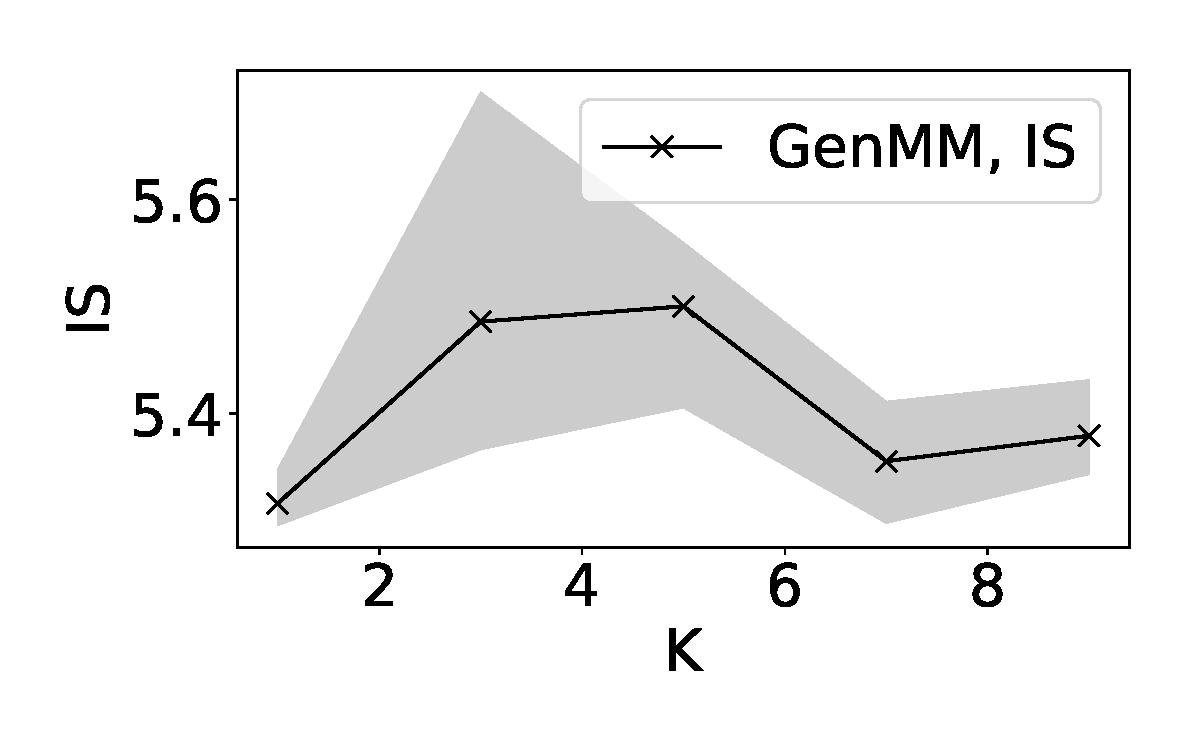
\includegraphics[width=1\linewidth]{images/fashion-mnist/scores/EMGM-NM/EMGM-NM-IS-K.pdf}
% %     \caption{IS score}
%     %     \label{fig-nm-isk}
%   \end{subfigure}
%   \vspace{-2pt}
%   \begin{subfigure}{.24\textwidth}
%     \centering
%     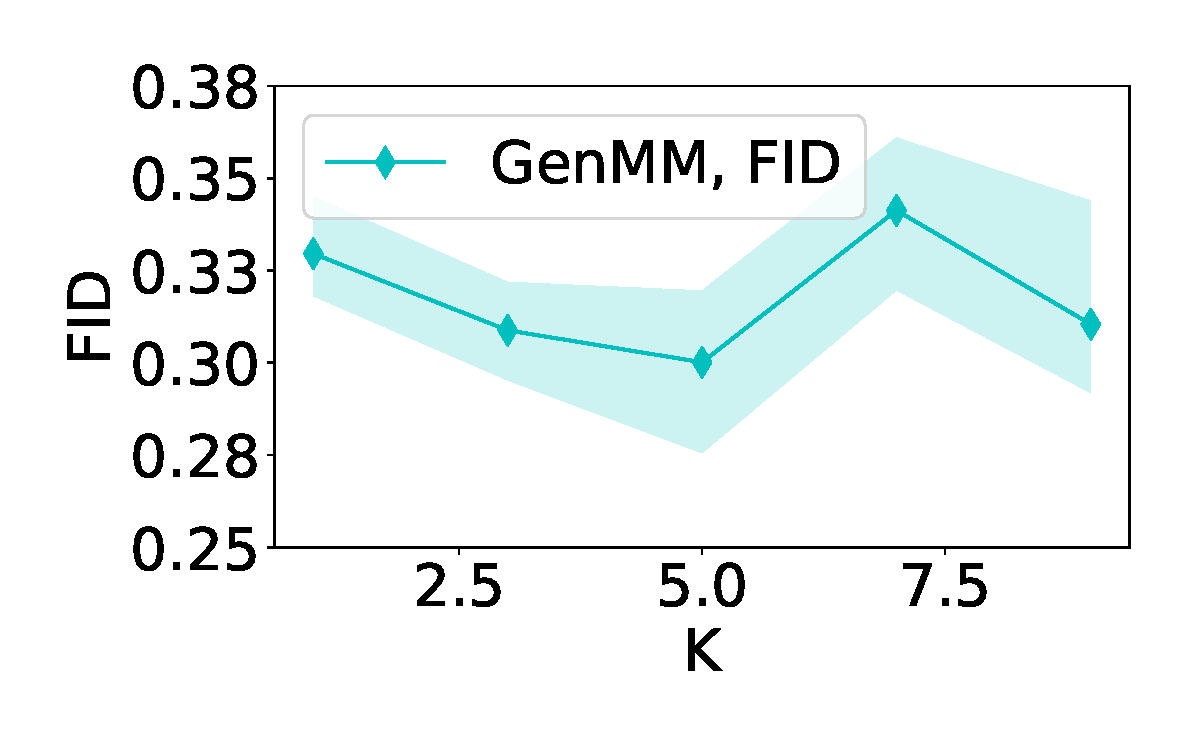
\includegraphics[width=1\linewidth]{images/fashion-mnist/scores/EMGM-NM/EMGM-NM-FID-K.pdf}
%     %     \caption{FID score}
%     %     \label{fig-nm-fidk}
%   \end{subfigure}
%   \centering
%   \begin{subfigure}{.24\textwidth}
%     \centering
%     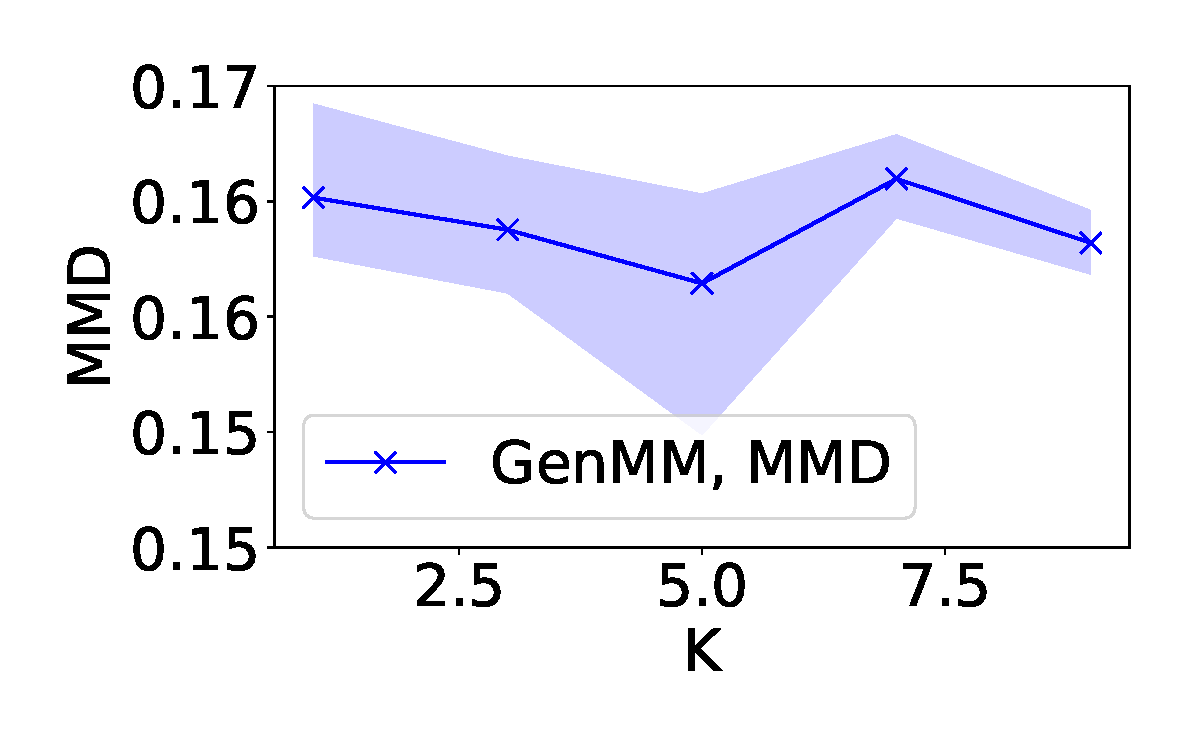
\includegraphics[width=1\linewidth]{images/fashion-mnist/scores/EMGM-NM/EMGM-NM-MMD-K.pdf}
%     %     \caption{MMD score}
%     %     \label{fig-nm-mmdk}
%   \end{subfigure}
%   \centering
%   \begin{subfigure}{0.24\textwidth}
%     \centering
%     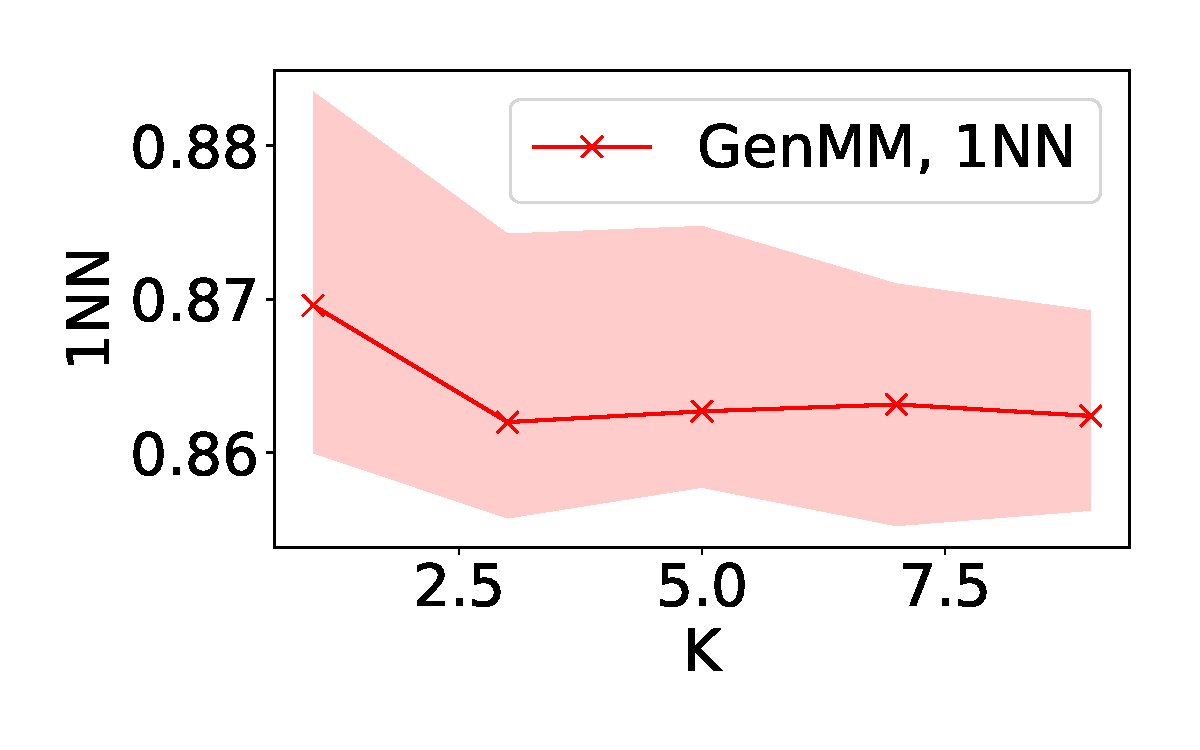
\includegraphics[width=1\linewidth]{images/fashion-mnist/scores/EMGM-NM/EMGM-NM-1NN-K.pdf}
%     %     \caption{1NN score}
%     %     \label{fig-nm-1nnk}
%   \end{subfigure}
%   \centering
%   \begin{subfigure}{.24\textwidth}
%     \centering
%     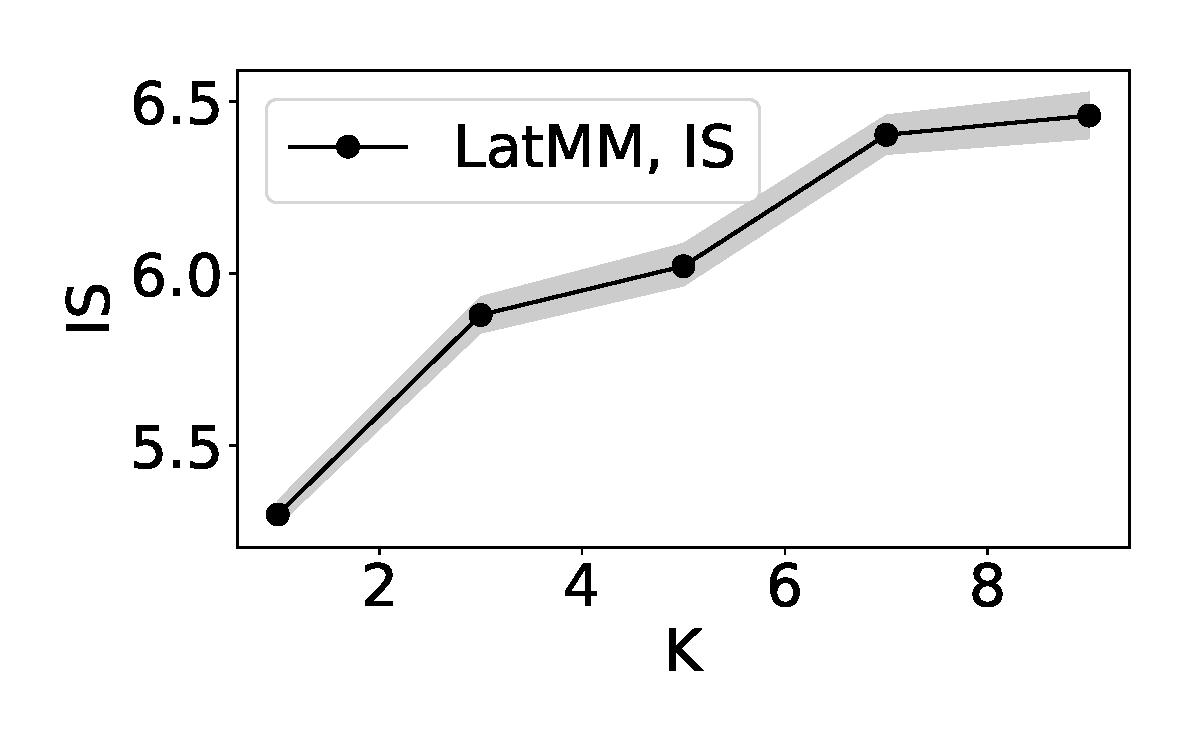
\includegraphics[width=1\linewidth]{images/fashion-mnist/scores/EMGM-SM/EMGM-SM-IS-K.pdf}
%     %     \caption{IS score}
%     %     \label{fig-sm-is}
%   \end{subfigure}
%   \centering
%   \begin{subfigure}{.24\textwidth}
%     \centering
%     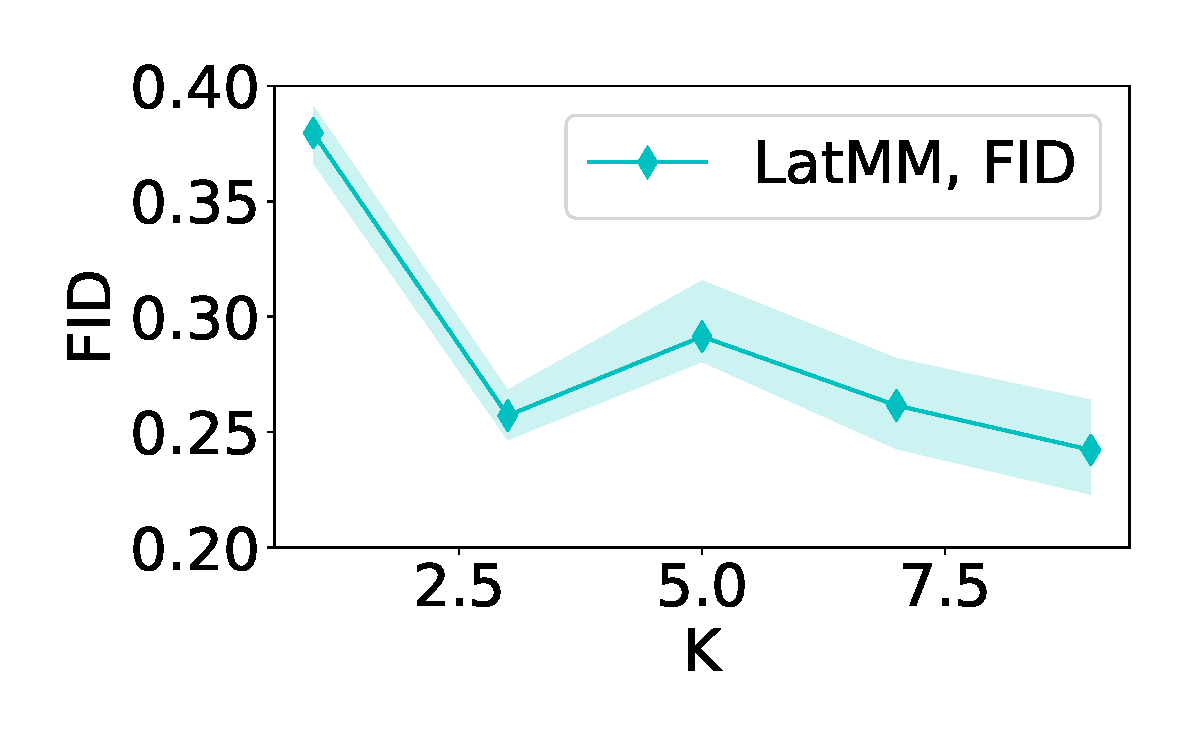
\includegraphics[width=1\linewidth]{images/fashion-mnist/scores/EMGM-SM/EMGM-SM-FID-K.pdf}
%     %     \caption{FID score}
%     %     \label{fig-sm-fid}
%   \end{subfigure}
%   \centering
%   \begin{subfigure}{.24\textwidth}
%     \centering
%     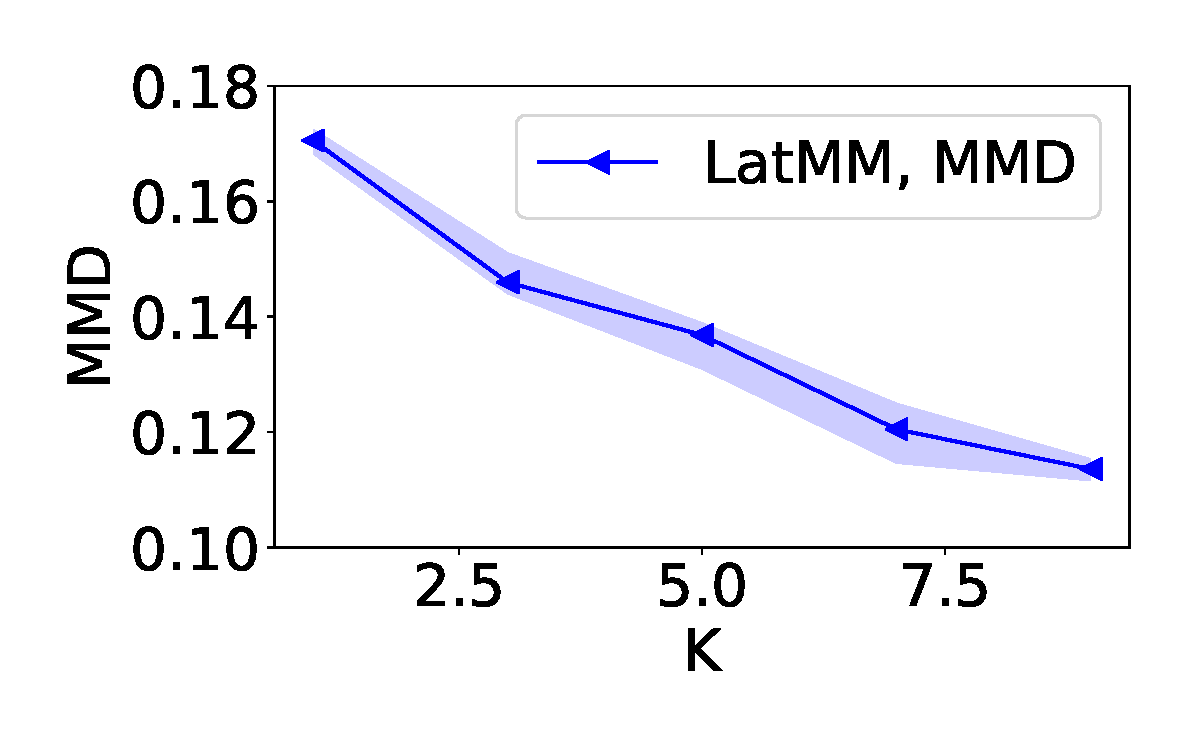
\includegraphics[width=1\linewidth]{images/fashion-mnist/scores/EMGM-SM/EMGM-SM-MMD-K.pdf}
%     %     \caption{MMD score}
%     %     \label{fig-sm-mmd}
%   \end{subfigure}
%   \begin{subfigure}{0.24\textwidth}
%     \centering
%     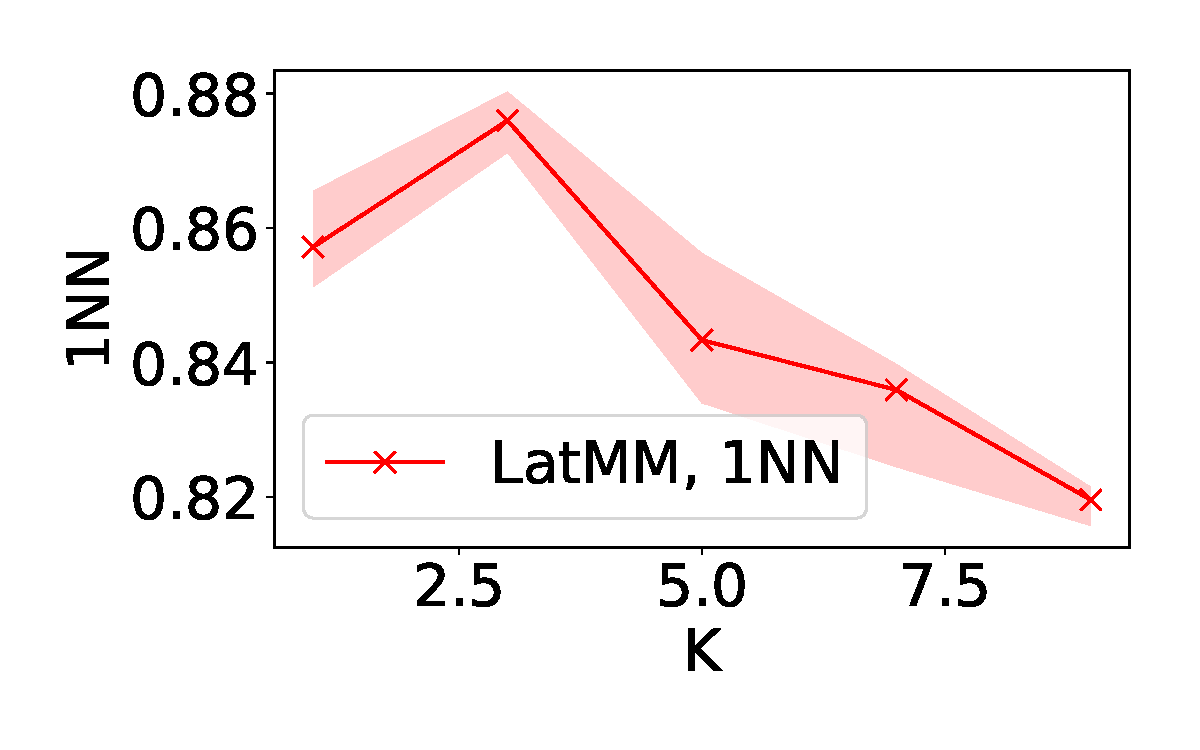
\includegraphics[width=1.\linewidth]{images/fashion-mnist/scores/EMGM-SM/EMGM-SM-1NN-K.pdf}
%     %     \caption{1NN score}
%     %     \label{fig-sm-1nn}
%   \end{subfigure}
%   \caption{ GenMM and LatMM evaluated on Fashion-MNIST (std =0.8) }
%   \vspace{10pt}
% \end{figure*}



In this section, we evaluate our proposed mixture models for generating samples and maximum likelihood classification. We will show encouraging results.

% under different metrics firstly. Then demos of sample generating and interpolation are shown. Lastly, we apply our model to classification tasks based on maximum likelihood criterion.

\begin{figure*}[!t]
  \captionsetup[subfigure]{justification=centering}
  \centering
  \begin{subfigure}{.4\textwidth}
    \centering
    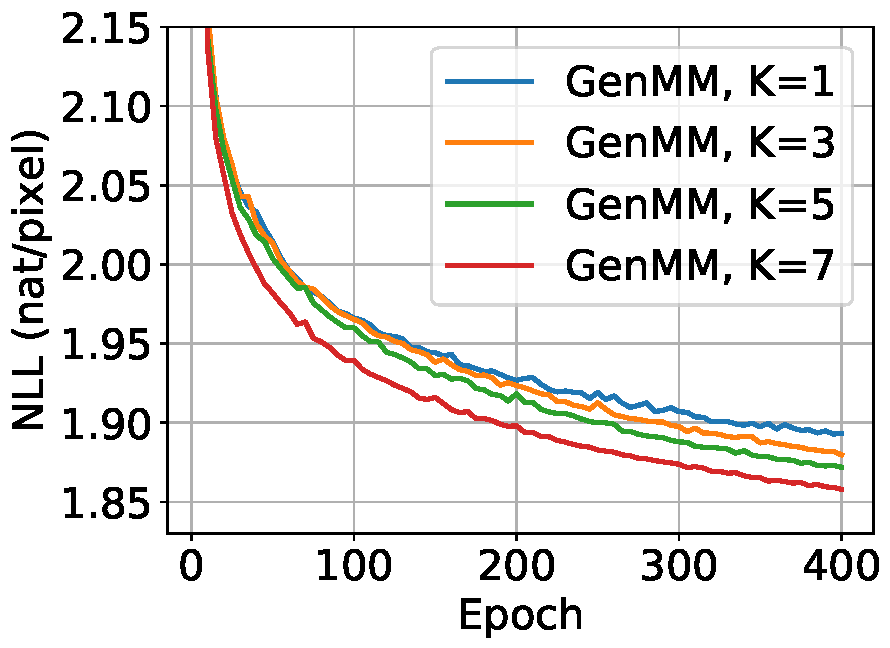
\includegraphics[width=1\linewidth]{images/supply/mnist_GenMM_nll_curves-crop.pdf}
    
    \caption{Dataset MNIST}
    \label{fig-genmm-mnist-nll-curve}
  \end{subfigure}\hspace{1cm}
  \begin{subfigure}{.4\textwidth}
    \centering
    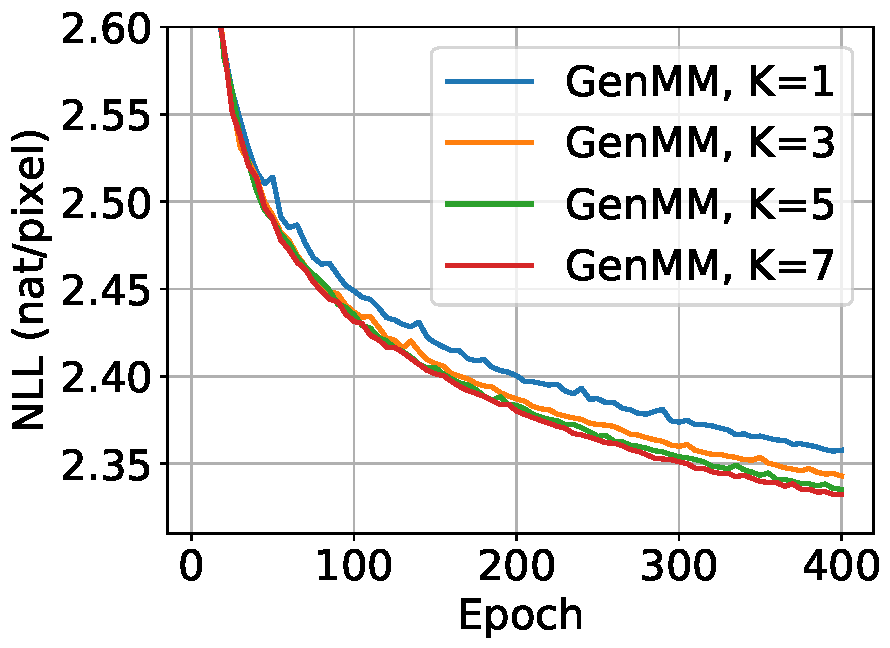
\includegraphics[width=1\linewidth]{images/supply/fashion_GenMM_nll_curves-crop.pdf}
    
    \caption{Dataset Fashion-MNIST}
    \label{fig-genmm-fsh-nll-curve}
  \end{subfigure}
  \caption{NLL (Unit: nat/pixel) of GenMM versus training epochs with different number of mixture component $K$. (a) $10000$ images from MNIST is used for training, (b) $10000$ images from Fashion-MNIST is used for training.}
  \label{fig:genmm-nll}
\end{figure*}

\begin{figure*}[!tp]
  \captionsetup[subfigure]{justification=centering}
  \centering
  \begin{subfigure}{.4\textwidth}
    \centering
    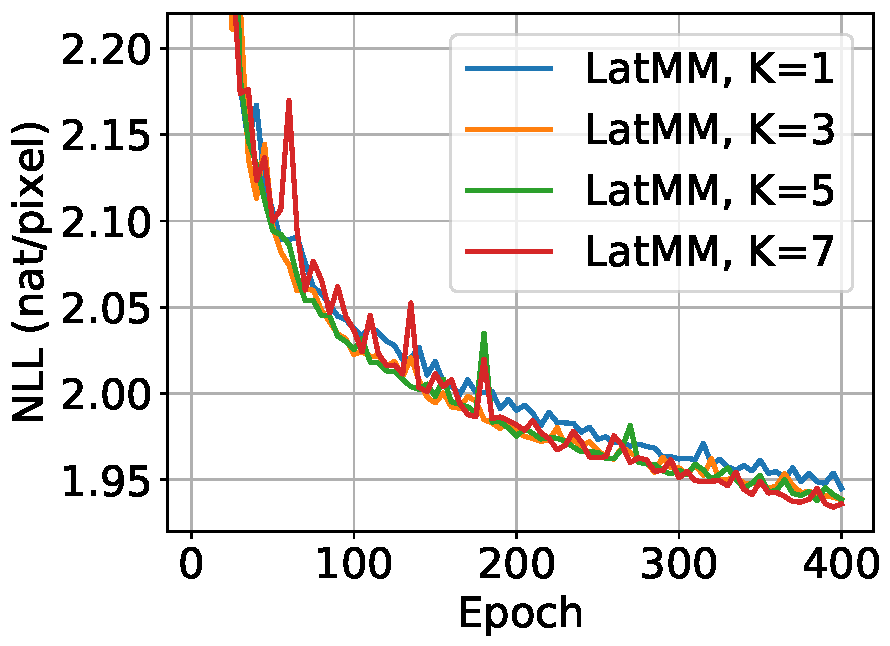
\includegraphics[width=1\linewidth]{images/supply/mnist_LatMM_nll_curves-crop.pdf}
    
    \caption{Dataset of MNIST}
    \label{fig-latmm-mnist-nll-curve}
  \end{subfigure}\hspace{1cm}
  \begin{subfigure}{.4\textwidth}
    \centering
    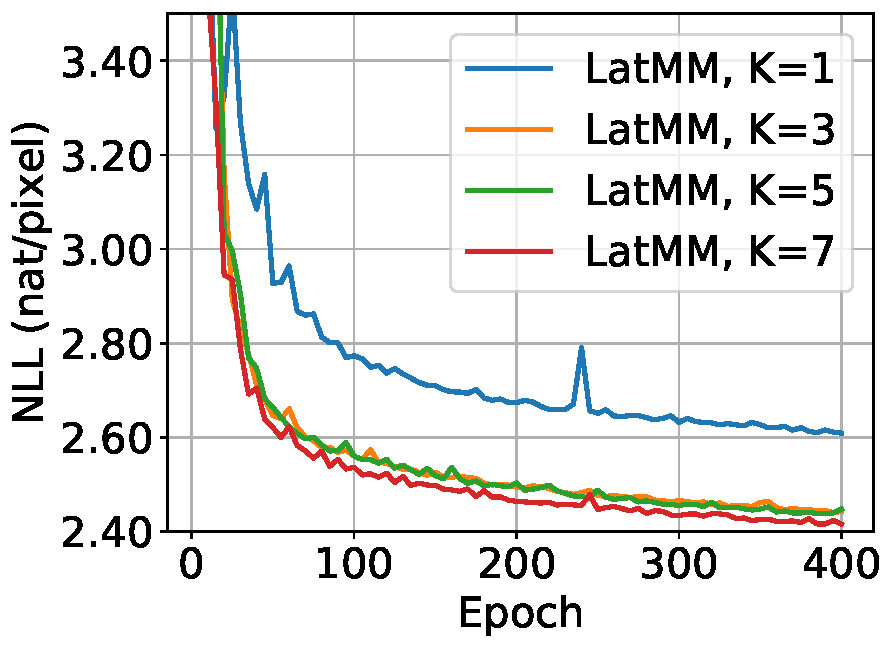
\includegraphics[width=1\linewidth]{images/supply/fashion_LatMM_nll_curves-crop.pdf}
    
    \caption{Dataset Fashion-MNIST}
    \label{fig-latmm-fsh-nll-curve}
  \end{subfigure}
  
  \caption{NLL (Unit: nat/pixel) of LatMM versus training epochs with different number of mixture component $K$. (a) $10000$ images from MNIST is used for training, (b) $10000$ images from Fashion-MNIST is used for training.}
  \label{fig:latmm-nll}
\end{figure*}


\subsection{Experimental setup}\label{sub:exp-setup}

We use the flow-based neural network for implementing generators $\{\bm{g}_k\}_{k=1}^{K}$ in GenMM and $\bm{g}$ in LatMM. Specifically, we use the Glow structure \cite{2018arXiv180703039K} that is developed based on RealNVP \cite{2016arXiv160508803D} and NICE \cite{DBLP:journals/corr/DinhKB14}. As introduced in Section~\ref{chpt6:sec:flow}, the operation in \eqref{chpt6:eq-gl-coupling} is a coupling
layer. Since only a part of the input is mapped non-linearly after a coupling
layer and the rest part remains the same, permutation \cite{2016arXiv160508803D} or $1\times 1$ convolution operation \cite{2018arXiv180703039K} is used to alternate the part of the signal that goes through identity mapping. In Glow structure, a basic \textit{flow step} is the concatenation of three layers: Actnorm (element-wise affine mapping)
$\rightarrow$ $1\times 1$ Convolution (for permutation purpose)
$\rightarrow$ Coupling layer. A \textit{flow block} consists of: a squeeze layer,
several flow steps, a split layer. A squeeze layer reshapes the
signal. A split layer allows the flow model to split some elements of hidden layers out and model them
directly as standard Gaussian, which relieves the computation burden. In our experiments, there are also split layers that make dimension of $\bm{z}$ one fourth of dimension $\bm{x}$, and split signals in hidden layers are modeled by standard Gaussian. 

% In all of our experiments, the generators $\bm{g}_k, \forall k$, in
% GenMM and $\bm{g}$ of LatMM use the same structure: \textit{three} flow blocks with
% each flow block consisting of \textit{four} coupling layers.  
All generators used in our experiments are randomly initialized before training. 
% In order to make comparison fair, our models with different configuration of $K$ are all trained for $30$ epochs on both datasets. Comparison are made with the trained models.  
In addition, the prior distribution $\bm{\pi}$ update in both GenMM and LatMM is every $5$ epochs, {i.e.},  $t_{\pi} = 5$. For the training of LatMM, we adopt the Gamma distribution $\Gamma(\bm{\sigma}_k^{-1}; a, b)$ as the parameter prior for $\bm{\sigma}_k^{-1}, \forall k$, with shape parameter $a=2$ and rate parameter $b = 1$.

\begin{figure*}[!tp]
  \captionsetup[subfigure]{justification=centering}
  \centering
  \begin{subfigure}{.24\textwidth}
    \centering
    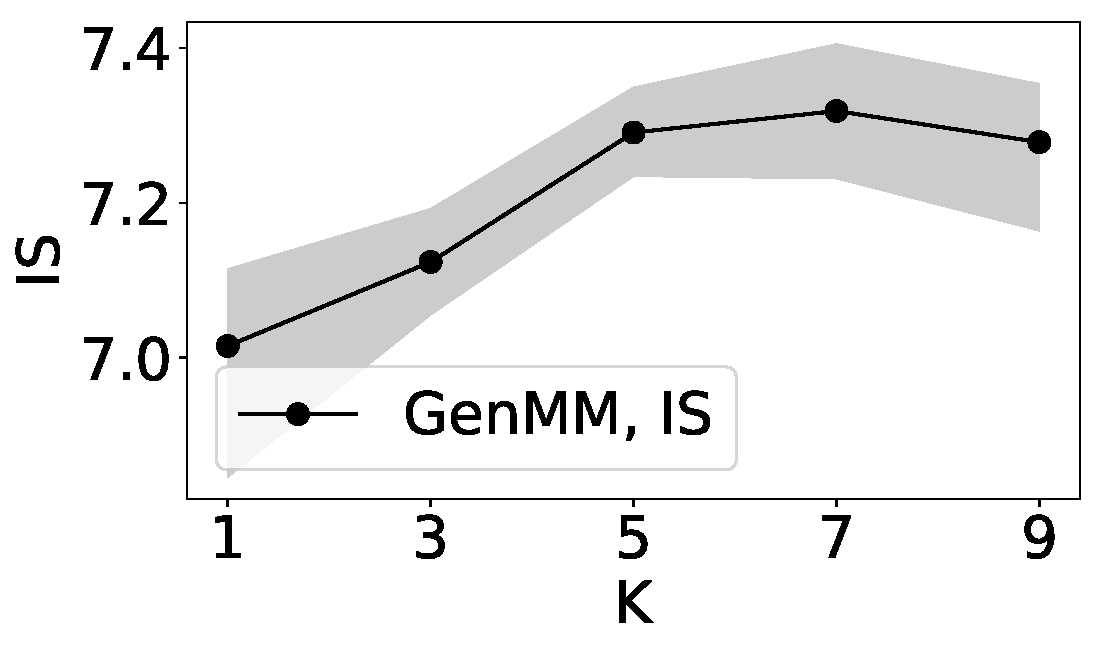
\includegraphics[width=1\linewidth]{images/mnist/scores/std1EMGM-NM/EMGM-NM-IS-K.pdf}
    % \caption{IS score}
    % \label{fig-nm-isk}
  \end{subfigure}
  \vspace{-2pt}
  \begin{subfigure}{.24\textwidth}
    \centering
    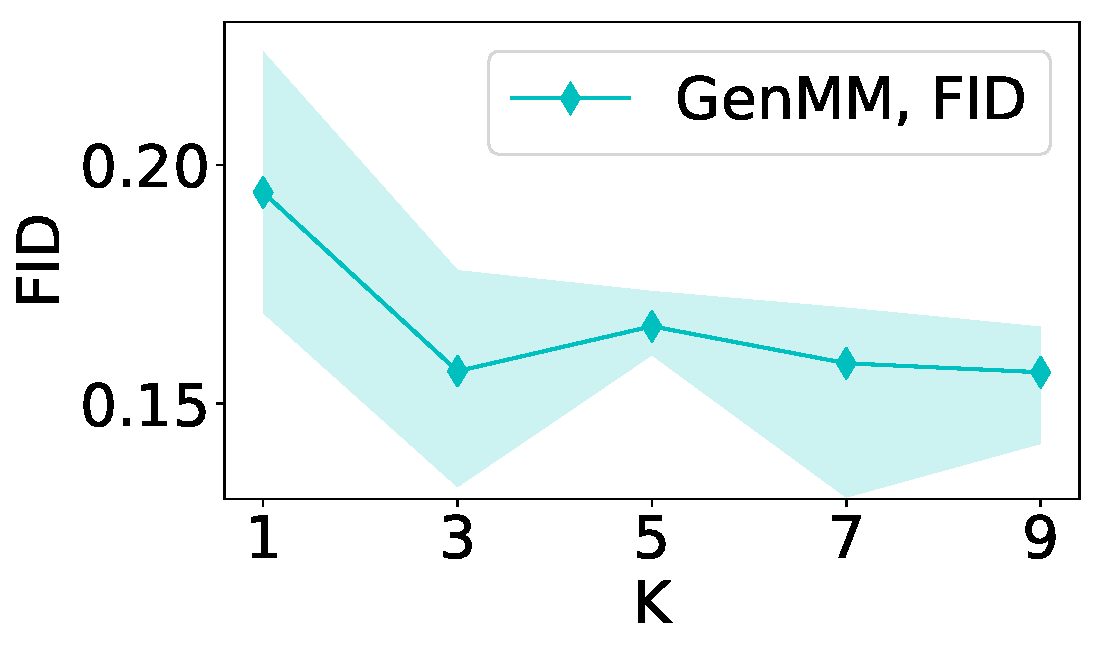
\includegraphics[width=1\linewidth]{images/mnist/scores/std1EMGM-NM/EMGM-NM-FID-K.pdf}
    % \caption{FID score}
    % \label{fig-nm-fidk}
  \end{subfigure}
  \centering
  \begin{subfigure}{.24\textwidth}
    \centering
    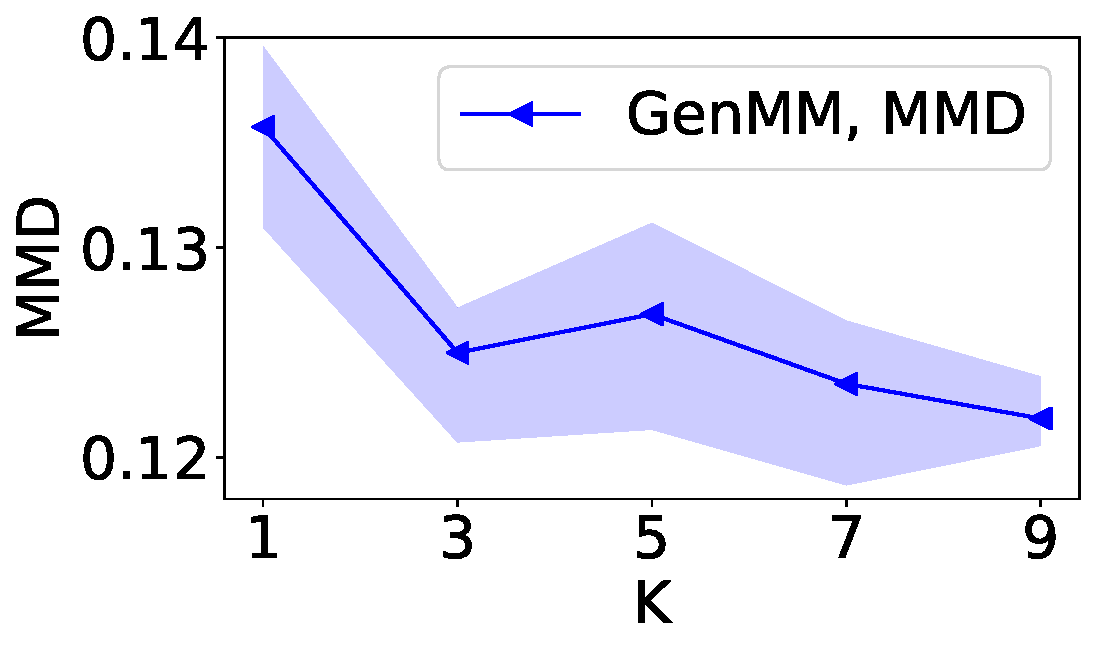
\includegraphics[width=1\linewidth]{images/mnist/scores/std1EMGM-NM/EMGM-NM-MMD-K.pdf}
    % \caption{MMD score}
    % \label{fig-nm-mmdk}
  \end{subfigure}
  \centering
  \begin{subfigure}{0.24\textwidth}
    \centering
    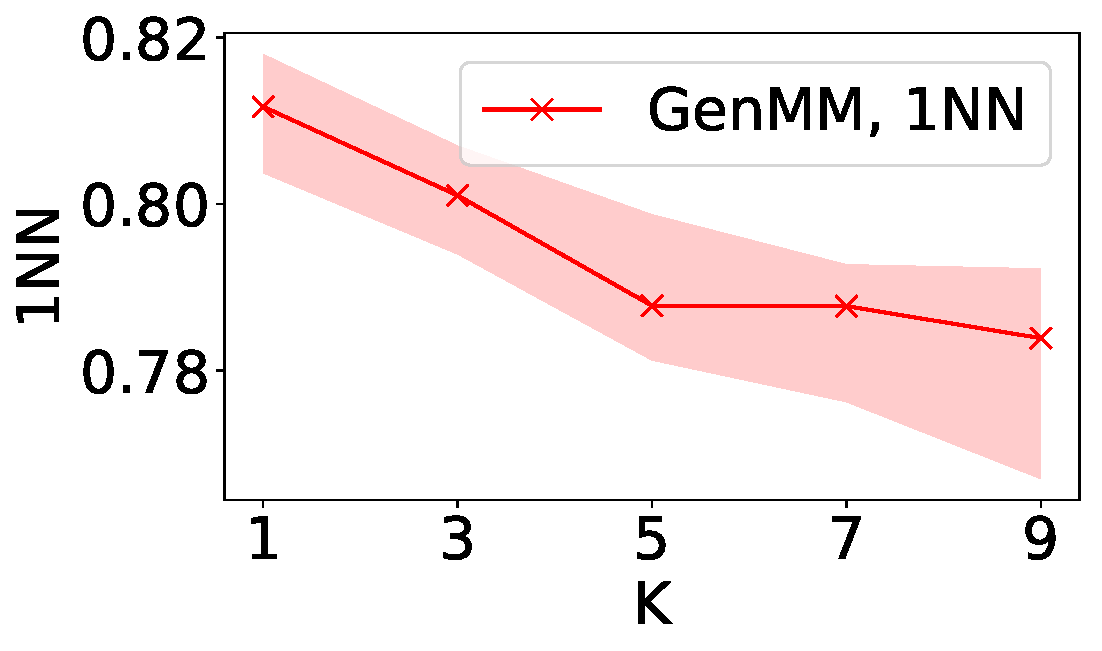
\includegraphics[width=1\linewidth]{images/mnist/scores/std1EMGM-NM/EMGM-NM-1NN-K.pdf}
    % \caption{1NN score}
    % \label{fig-nm-1nnk}
  \end{subfigure}
  \centering
  \begin{subfigure}{.24\textwidth}
    \centering
    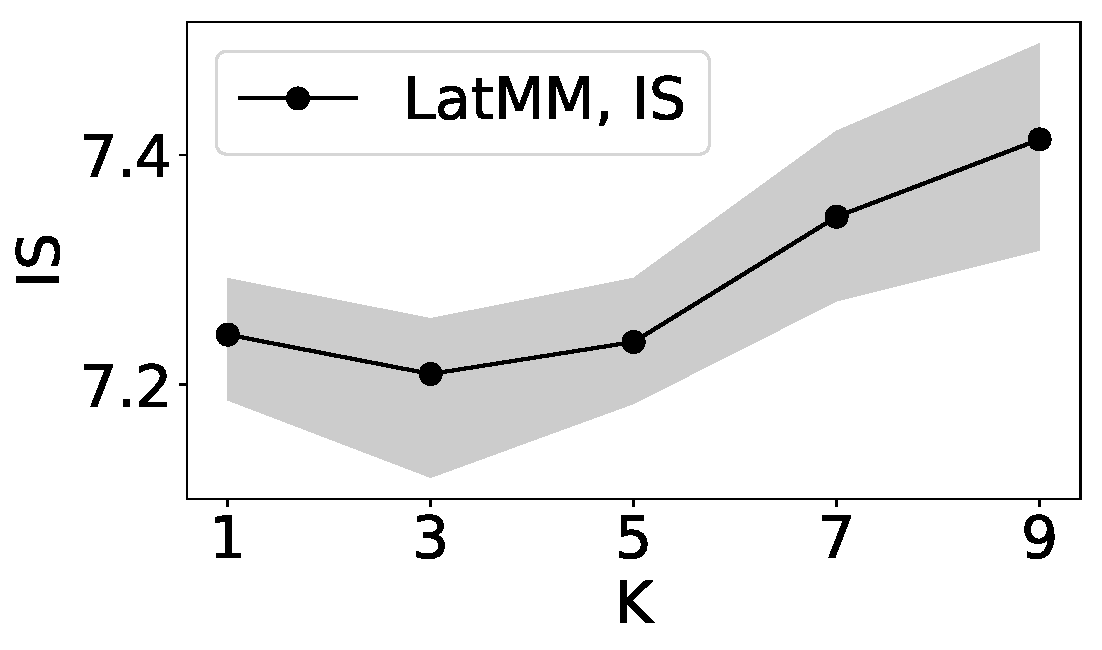
\includegraphics[width=1\linewidth]{images/mnist/scores/std1EMGM-SM/EMGM-SM-IS-K.pdf}
    % \caption{IS score}
    % \label{fig-sm-is}
  \end{subfigure}
  \centering
  \begin{subfigure}{.24\textwidth}
    \centering
    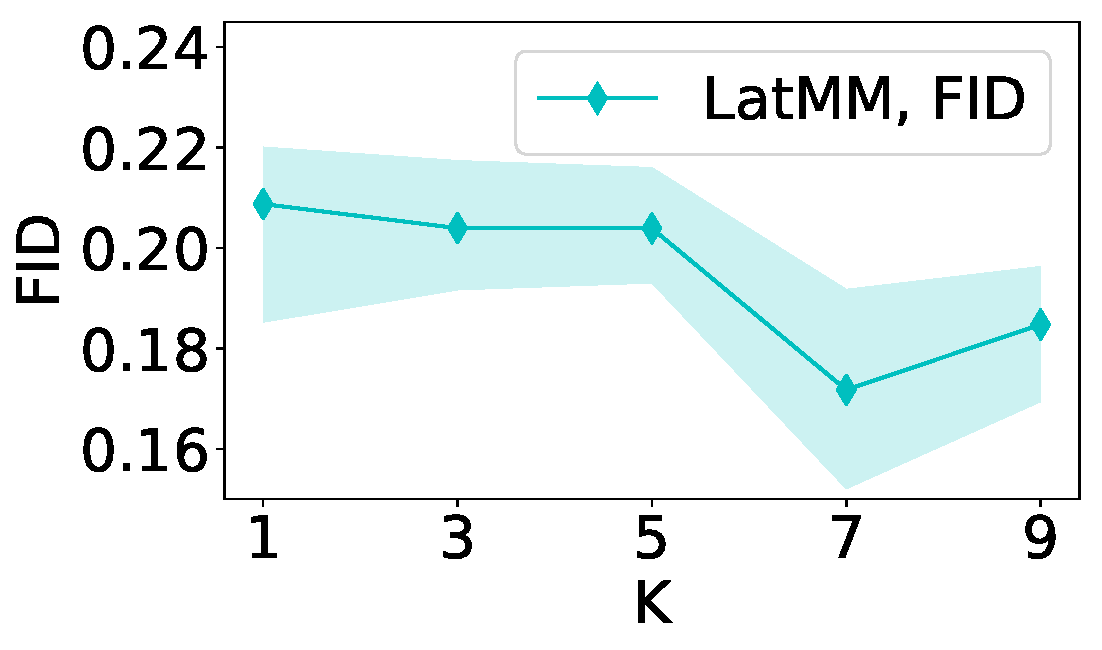
\includegraphics[width=1\linewidth]{images/mnist/scores/std1EMGM-SM/EMGM-SM-FID-K.pdf}
    % \caption{FID score}
    % \label{fig-sm-fid}
  \end{subfigure}
  \centering
  \begin{subfigure}{.24\textwidth}
    \centering
    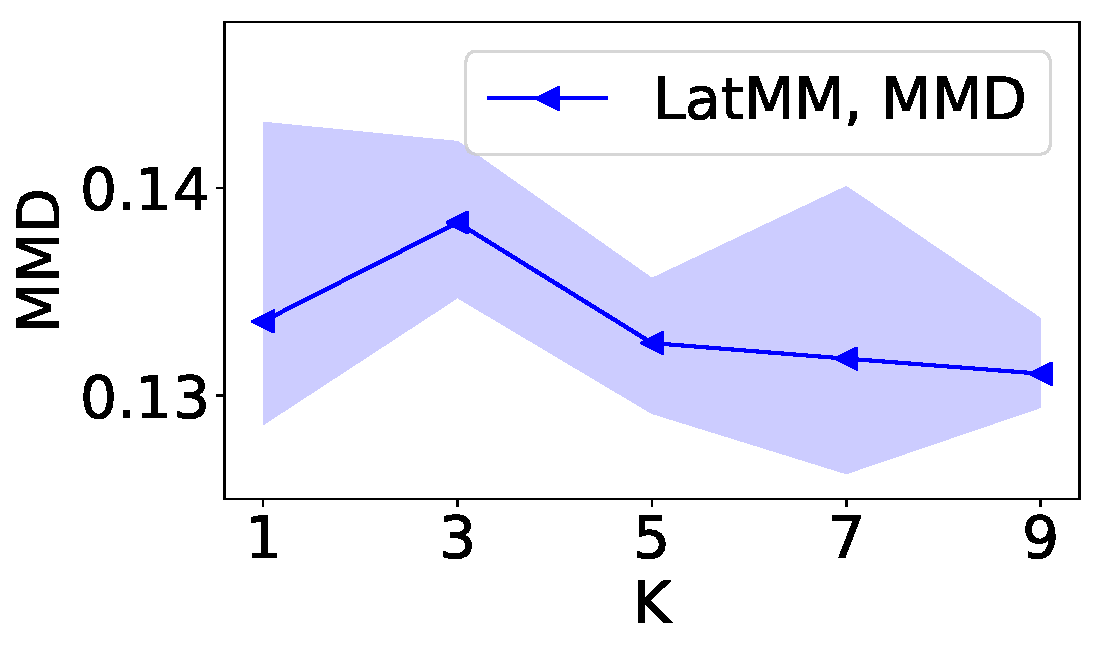
\includegraphics[width=1\linewidth]{images/mnist/scores/std1EMGM-SM/EMGM-SM-MMD-K.pdf}
    % \caption{MMD score}
    % \label{fig-sm-mmd}
  \end{subfigure}
  \begin{subfigure}{0.24\textwidth}
    \centering
    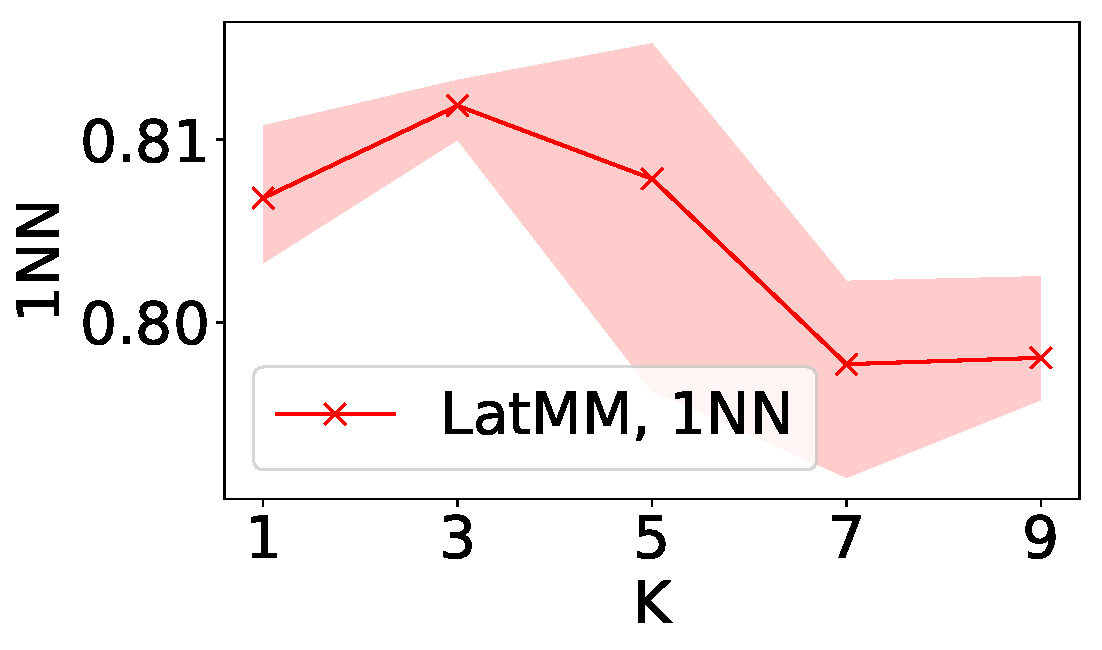
\includegraphics[width=1.\linewidth]{images/mnist/scores/std1EMGM-SM/EMGM-SM-1NN-K.pdf}
    % \caption{1NN score}
    % \label{fig-sm-1nn}
  \end{subfigure}
  \caption{IS, FID, MMD and 1NN of GenMM and LatMM for MNIST dataset. GenMM and LatMM are trained on $60000$ images of MNIST. The results are evaluated on $2000$ samples per simulation point ($1000$ samples generated by GenMM or LatMM for corresponding $K$, $1000$ samples from MNIST). $5$ experiments are carried out for each assessed score at each setting of $K$. Curve with marker denotes mean score and shaded area denotes the range of corresponding score.}\label{fig-scores-k}
\end{figure*}

\begin{figure*}[!ht]
  \captionsetup[subfigure]{justification=centering}
  \centering
  \begin{subfigure}{.24\textwidth}
    \centering
    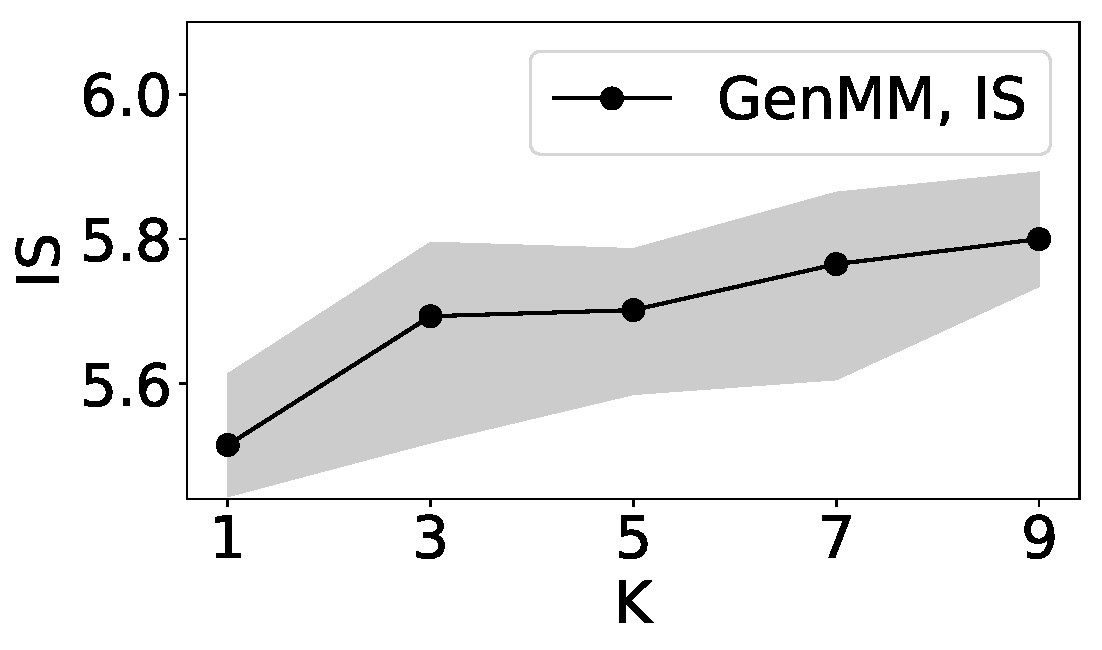
\includegraphics[width=1.0\linewidth]{images/fashion-mnist/scores/std1EMGM-NM/EMGM-NM-IS-K.pdf}
    % \caption{IS score}
    % \label{fig-nm-isk}
  \end{subfigure}
  \vspace{-2pt}
  \begin{subfigure}{.24\textwidth}
    \centering
    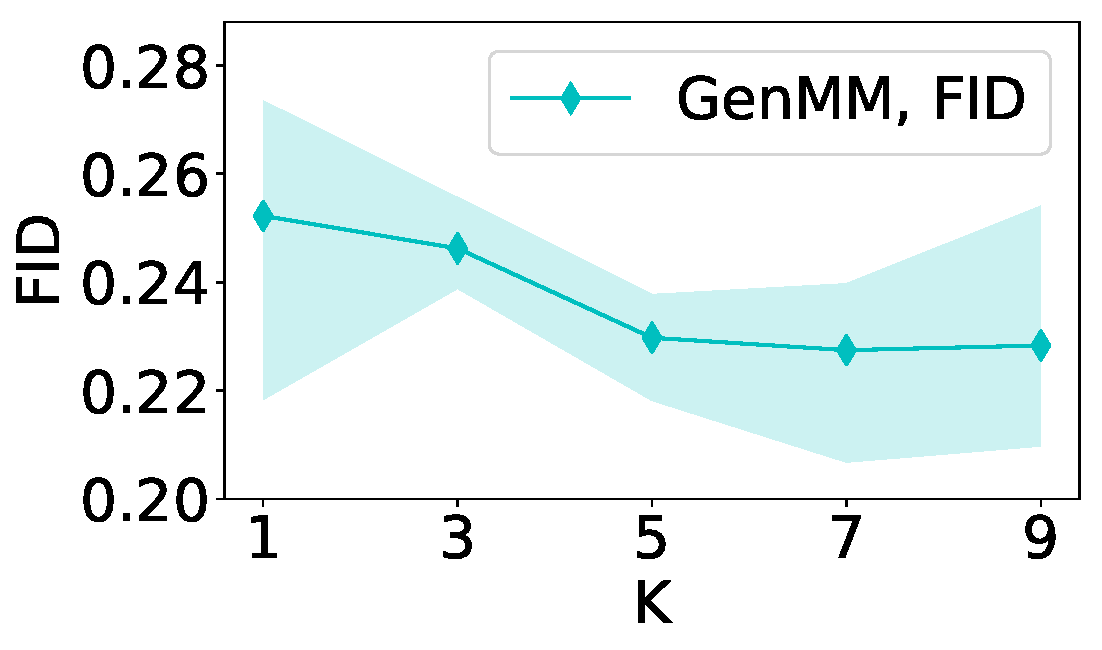
\includegraphics[width=1.0\linewidth]{images/fashion-mnist/scores/std1EMGM-NM/EMGM-NM-FID-K.pdf}
    % \caption{FID score}
    % \label{fig-nm-fidk}
  \end{subfigure}
  \centering
  \begin{subfigure}{.24\textwidth}
    \centering
    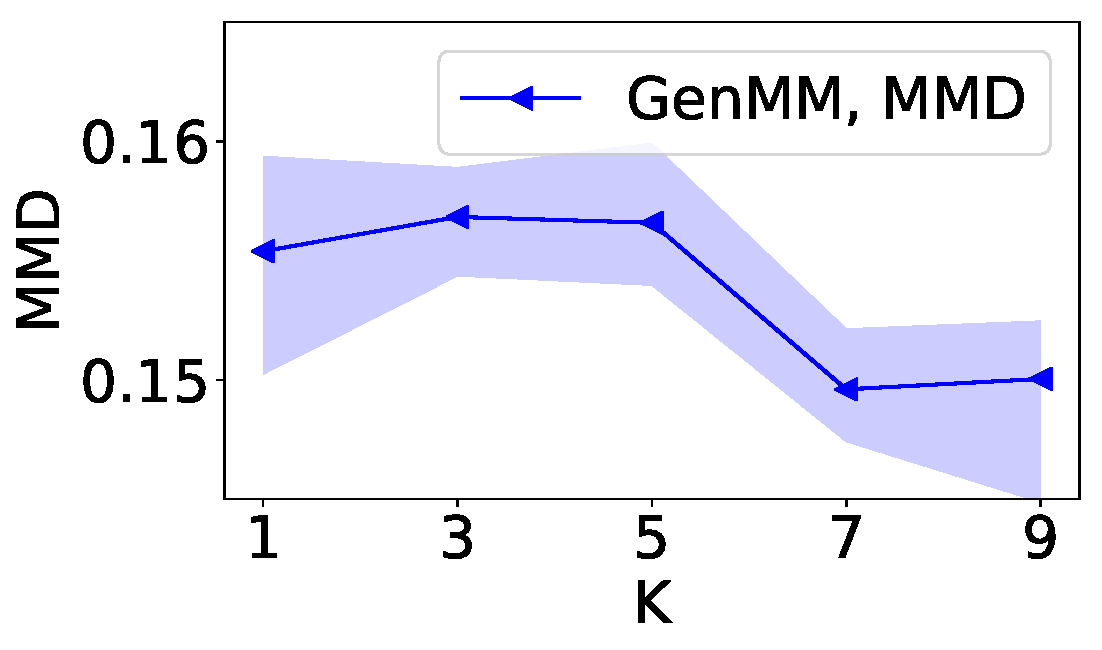
\includegraphics[width=1\linewidth]{images/fashion-mnist/scores/std1EMGM-NM/EMGM-NM-MMD-K.pdf}
    % \caption{MMD score}
    % \label{fig-nm-mmdk}
  \end{subfigure}
  \centering
  \begin{subfigure}{0.24\textwidth}
    \centering
    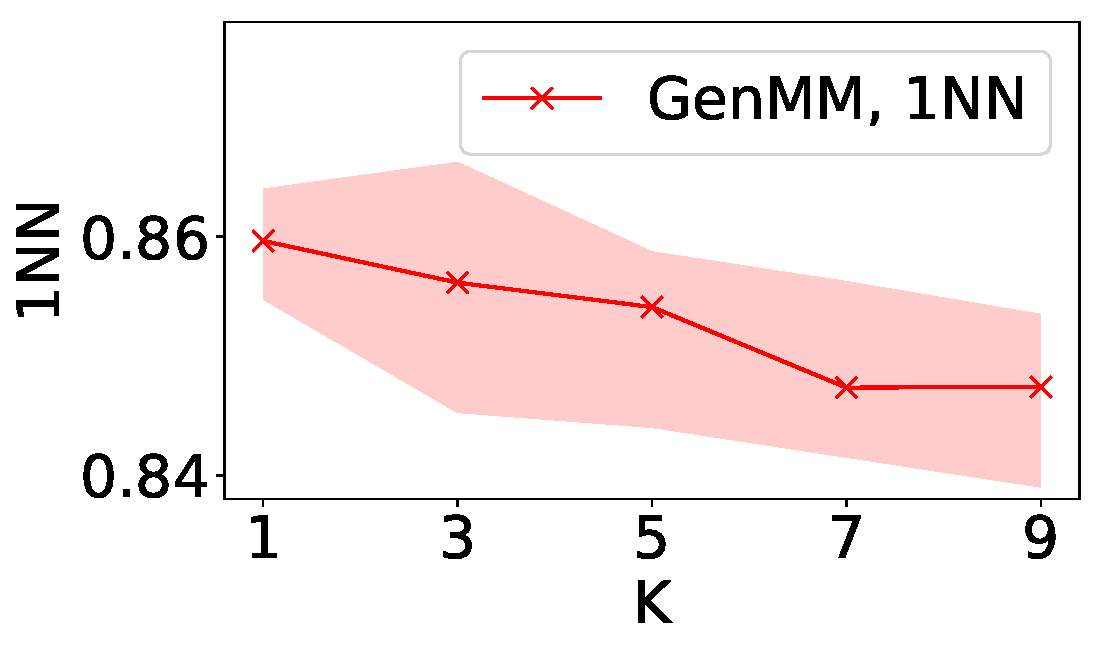
\includegraphics[width=1\linewidth]{images/fashion-mnist/scores/std1EMGM-NM/EMGM-NM-1NN-K.pdf}
    % \caption{1NN score}
    % \label{fig-nm-1nnk}
  \end{subfigure}
  \centering
  \begin{subfigure}{.24\textwidth}
    \centering
    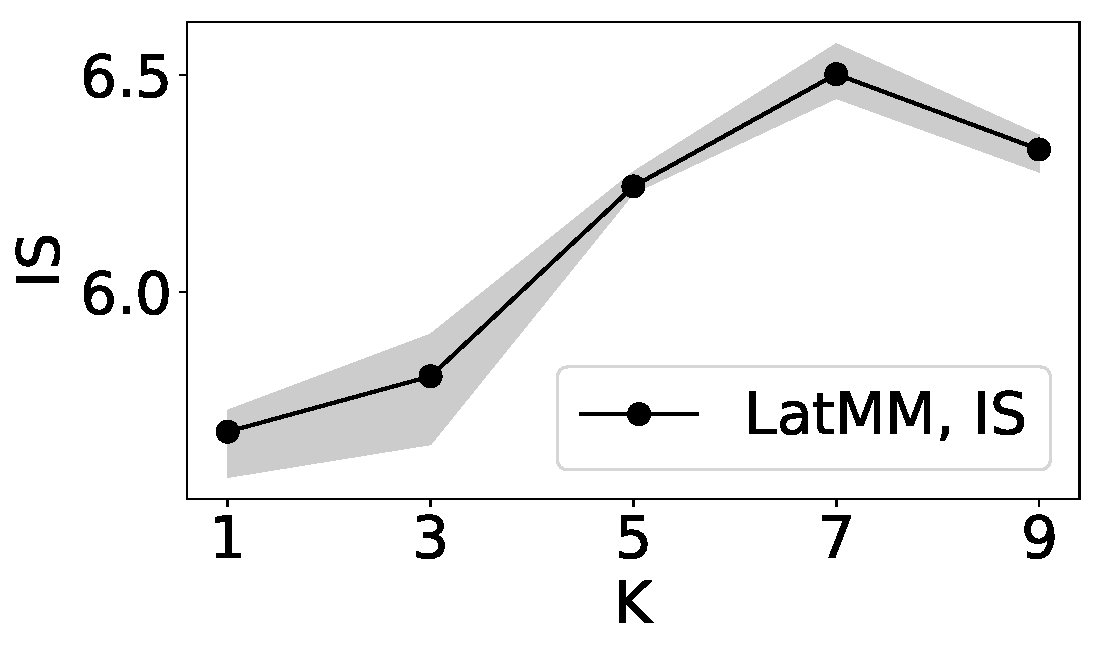
\includegraphics[width=1\linewidth]{images/fashion-mnist/scores/std1EMGM-SM/EMGM-SM-IS-K.pdf}
    % \caption{IS score}
    % \label{fig-sm-is}
  \end{subfigure}
  \centering
  \begin{subfigure}{.24\textwidth}
    \centering
    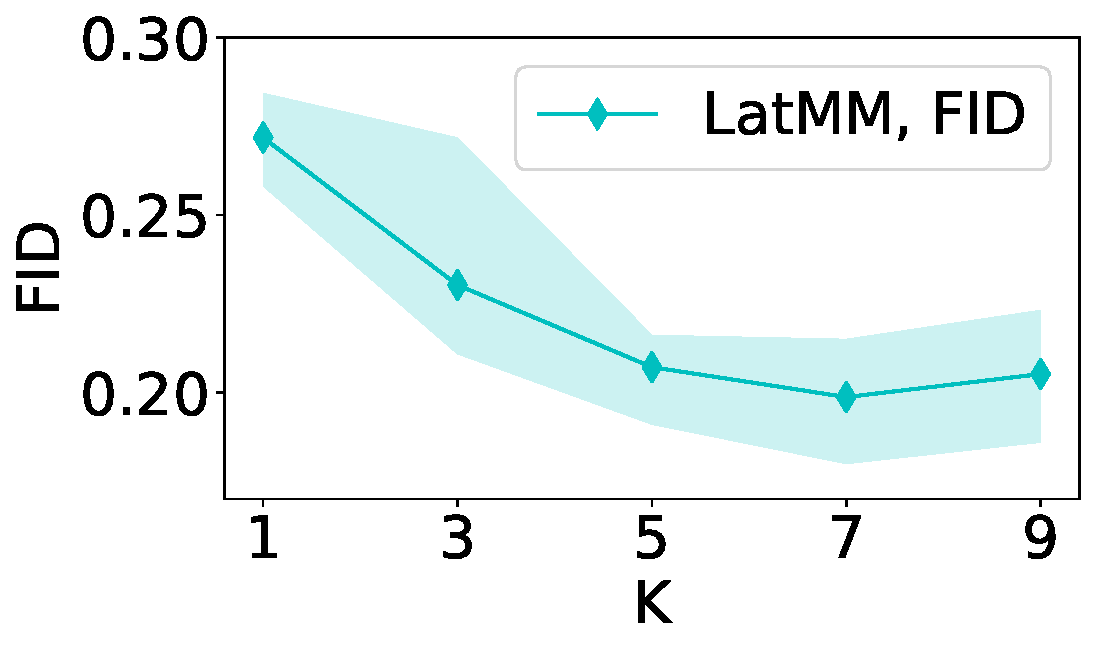
\includegraphics[width=1\linewidth]{images/fashion-mnist/scores/std1EMGM-SM/EMGM-SM-FID-K.pdf}
    % \caption{FID score}
    % \label{fig-sm-fid}
  \end{subfigure}
  \centering
  \begin{subfigure}{.24\textwidth}
    \centering
    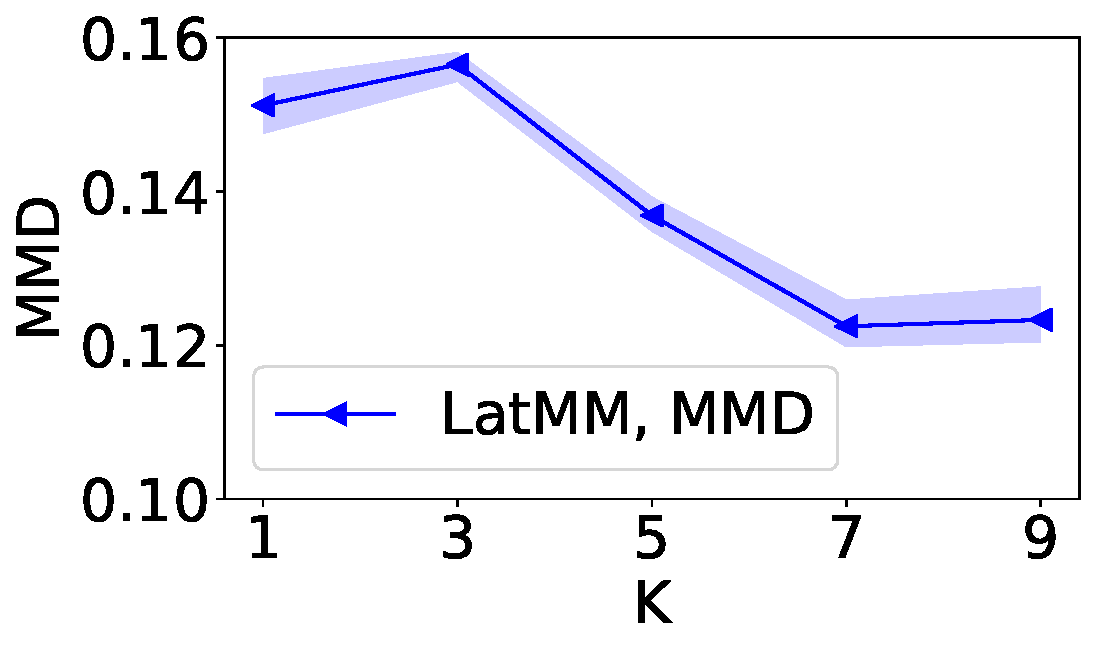
\includegraphics[width=1\linewidth]{images/fashion-mnist/scores/std1EMGM-SM/EMGM-SM-MMD-K.pdf}
    % \caption{MMD score}
    % \label{fig-sm-mmd}
  \end{subfigure}
  \begin{subfigure}{0.24\textwidth}
    \centering
    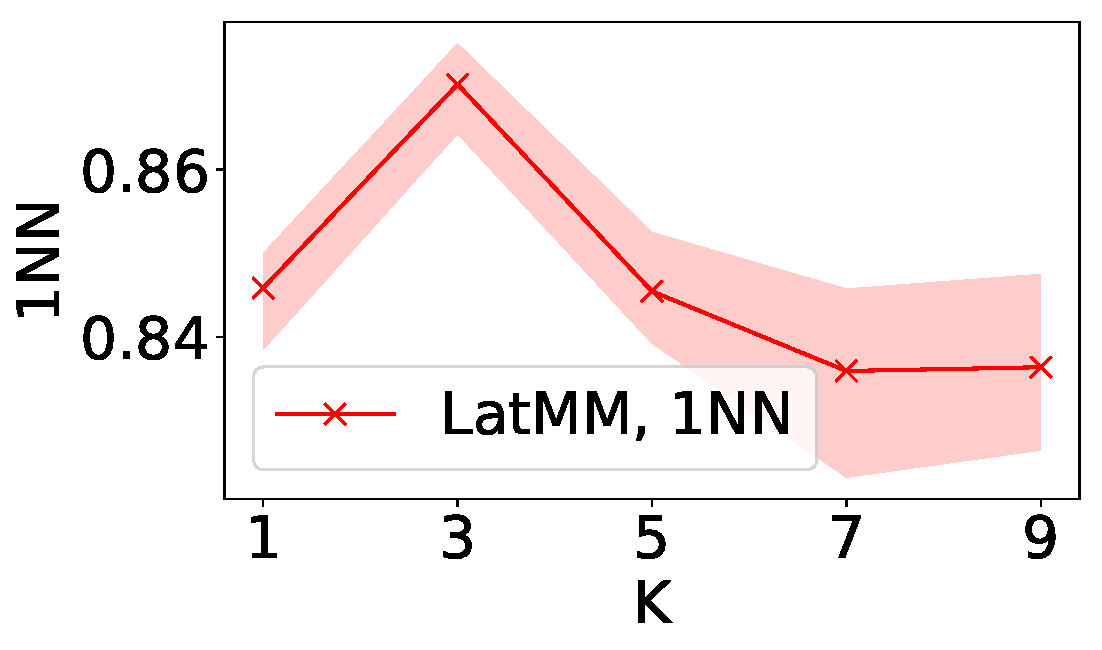
\includegraphics[width=1.\linewidth]{images/fashion-mnist/scores/std1EMGM-SM/EMGM-SM-1NN-K.pdf}
    % \caption{1NN score}
    % \label{fig-sm-1nn}
  \end{subfigure}
  \caption{IS, FID, MMD and 1NN of GenMM and LatMM for
    Fashion-MNIST dataset. GenMM and LatMM are trained on $60000$ images of Fashion-MNIST. The results are evaluated on $2000$ samples
    per simulation point ($1000$ samples generated by GenMM or LatMM
    for corresponding $K$, $1000$ samples from Fashion-MNIST). $5$
    experiments are carried out for each assessed score at each
    setting of $K$. Curve with marker denotes mean score and shaded
    area denotes the range of corresponding
    score.}\label{fig-scores-k-FashionMNIST}
\end{figure*}

\subsection{Evaluation of Proposed Models}\label{chpt6:sec:eval-metrics}
In order to see if the proposed algorithms of GenMM and LatMM help to improve the probability distribution modeling capacity, we assess our proposed algorithms with varying number of mixtures ($K$). Since our models are explicit models, the negative log likelihood (NLL) is used for comparison of our models. Apart from NLL, another four different metrics are used in the assessment of models.
The metrics are Inception Score (IS) \cite{NIPS2016_6125,2018arXiv180101973B,2018arXiv180607755X}, Frechet
Inception Distance (FID) \cite{2017arXiv170608500H}, Maximum Mean
Discrepancy (MMD) \cite{2018arXiv180607755X} and two-sample test based 1-Nearest
Neighbor (1NN) score \cite{2016arXiv161006545L}. IS measures statistically if a given sample can be recognized by a classifier with high confidence. A high IS stands for high quality for generated samples. FID measures a divergence between two distributions under testing by assuming these two distributions are both Gaussian. We also use MMD with Gaussian kernel to test how dissimilar two distributions are.
Small values of FID and MMD mean that the mixture distribution model
is close to the underlying distribution of the dataset. 1NN score measures
if two given distributions are empirically close by computing 1NN accuracy
on samples from two distributions under testing. The closer 1NN score is to $0.5$, the more likely 
two distributions under testing are the same. Therefore, a high IS is good, low FID and MMD scores, and 1NN score close to 0.5 are good. We use the evaluation
framework of \cite{2018arXiv180607755X} to compute these metrics scores, where
we train a ResNet on datasets MNIST and Fashion-MNIST, respectively, as the feature extractor for evaluation of the four performance metrics.



\begin{table}
  \caption{The lowest NLL value of GenMM for curves in Figure~\ref{fig:genmm-nll} (nat/pixel).}
  \label{tab:lowestNLLgenMM}
   \centering
  \begin{tabular}{lcccc}
    \toprule
    {Dataset} & K=1 &  K=3 &  K=5 &  K=7 \\                                         
    \midrule                                                                                          MNIST &     1.8929 &    1.8797 &    1.8719 &    1.8579 \\
    FashionMNIST &   2.3571 &   2.3429 &   2.3353 &   2.3323 \\
    \bottomrule
  \end{tabular} 
\end{table}

The NLL curves of GenMM and LatMM models during model training phase are shown in Figure~\ref{fig:genmm-nll} and Figure~\ref{fig:latmm-nll}, respectively. Subsets of MNIST and Fashion-MNIST are used to train our mixture models in order to assess their performance with regard to NLL when a different number of mixture components $K$ is used. All the curves in Figure~\ref{fig:genmm-nll} and Figure~\ref{fig:latmm-nll} show that NLL decreases as the training epoch number increases in general. There is fluctuation of these decreasing NLL curves due to: (a) the iteration of E-step and M-step of EM, and (b) the use of batch-size gradient in the optimization at the M-step. In each figure of Figure~\ref{fig:genmm-nll} and Figure~\ref{fig:latmm-nll}, a NLL curve corresponding to a larger total number of mixture components, $K$, reaches a smaller NLL value after training for the same number of epochs. The results are consistent since as $K$ increases, both GenMM and LatMM have smaller NLL. These results are consistent with our common sense that mixture models fit real data better. The lowest NLL values of curves in Figure~\ref{fig:genmm-nll} in training GenMM models are reported in Figure~\ref{tab:lowestNLLgenMM}.

\begin{figure*}[!t]
  \captionsetup[subfigure]{justification=centering}
  \centering
  \begin{subfigure}[b]{0.24\textwidth}
    \centering
    % 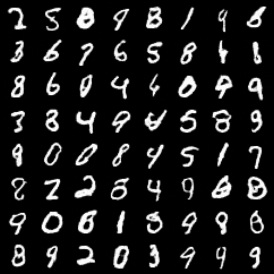
\includegraphics[width=1\linewidth]{images/mnist/samples/gen_c12_std08.png}
    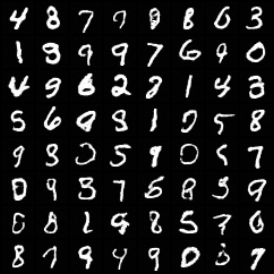
\includegraphics[width=1\linewidth]{images/mnist/samples/genMNIST_GenMM_K7_std089.png}
    \caption{Generated Samples. (GenMM, K=7)}
  \end{subfigure}
  % \begin{subfigure}[b]{0.19\textwidth}
  %   \centering
  %   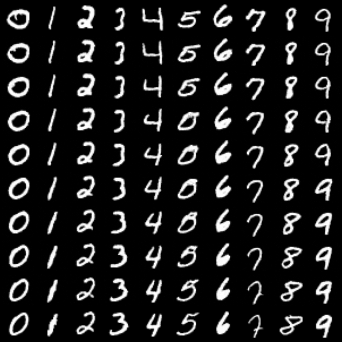
\includegraphics[width=1\linewidth]{images/mnist/interpolation/interpo_c12_mnist_std07.png}
  %   \caption{Interpolation. (GenMM, K=12)}\label{fig-interpo}
  % \end{subfigure}
  \centering
  \begin{subfigure}[b]{0.24\textwidth}
    \centering
    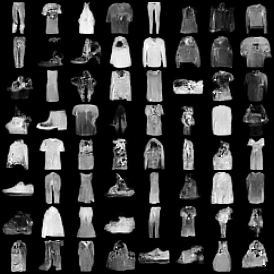
\includegraphics[width=1\linewidth]{images/fashion-mnist/samples/gene_c3_std1_samples.png}
    \caption{Generated samples. (GenMM, K=3)}
  \end{subfigure}
  \begin{subfigure}[b]{0.24\textwidth}
    \centering
    % 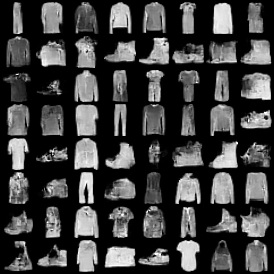
\includegraphics[width=1\linewidth]{images/fashion-mnist/samples/gen_s5_std1.png}
    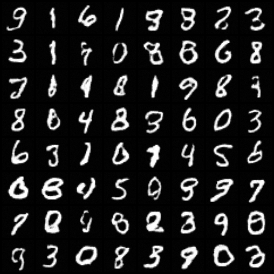
\includegraphics[width=1\linewidth]{images/mnist/samples/gen_LatMM_K3_std088.png}
    \caption{Generated samples. (LatMM, K=3)}
  \end{subfigure}
  \begin{subfigure}[b]{0.24\textwidth}
    \centering
    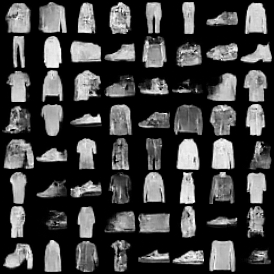
\includegraphics[width=1\linewidth]{images/fashion-mnist/samples/gen_s7_std1.png}
    \caption{Generated samples. (LatMM, K=7)}
  \end{subfigure}
  % \begin{subfigure}[b]{0.23\textwidth}
  %   \centering
  %   \includegraphics[width=1\linewidth]{images/fashion-mnist/samples/gene_c7_std1_samples.png}
  %   \caption{Generated samples. (EMGM-NM, K=7)}
  % \end{subfigure}
  \caption{Generated samples by GenMM and LatMM for MNIST and Fashion-MNIST datasets.}\label{fig-demo-samples}
\end{figure*}
      
\begin{figure*}[!t]
  \centering
  \captionsetup[subfigure]{justification=centering}
  \begin{subfigure}[b]{0.3\textwidth}
    \centering
    \includegraphics[width=1\linewidth]{images/mnist/interpolation/interpoMNIST_homo_GenMM_K7_map_grid.png}
    \caption{Interpolation by GenMM, K=7. Identity of $\bm{g}_k$ is chosen by $\argmax_{k}\; \gamma_k$.}\label{fig-interpo-genmm1}
  \end{subfigure}
  \hspace{10pt}
  \begin{subfigure}[b]{0.3\textwidth}
    \centering
    \includegraphics[width=1\linewidth]{images/mnist/interpolation/interpoMNIST_GenMM_K7_random_grid.png}
    \caption{Interpolation by GenMM, K=7. Identity of $\bm{g}_k$ is randomly chosen.~~~~~~~~~}\label{fig-interpo-genmm2}
  \end{subfigure}
  \hspace{10pt}
  \begin{subfigure}[b]{0.3\textwidth}
    \centering
    \includegraphics[width=1\linewidth]{images/fashion-mnist/interpolation/interpoFashion_homo_GenMM_K9_map_grid.png}
    \caption{Interpolation by GenMM, K=9. Identity of $\bm{g}_k$ is chosen by $\argmax_{k}\; \gamma_k$.}\label{fig-interpo-genmm3}
  \end{subfigure}
  % \caption{Interpolation in latent space to generate samples . GenMM}\label{fig-interpo}
  \vspace{0.22cm}
  % \label{fig-app-interpolation}
  % \vspace{0.2cm}
  % \end{figure*}
  % \begin{figure*}[!ht]
  \centering
  \captionsetup[subfigure]{justification=centering}
  \begin{subfigure}[b]{0.3\textwidth}
    \centering
    \includegraphics[width=1\linewidth]{images/mnist/interpolation/LatMMK9interpo_sample_grid.png}
    \caption{Interpolation by LatMM, K=9.}\label{fig-interpo-latmm1}
  \end{subfigure}
  \hspace{10pt}
  \begin{subfigure}[b]{0.3\textwidth}
    \centering
    \includegraphics[width=1\linewidth]{images/mnist/interpolation/interpoMNIST_heter_LatMM_K9_sample_grid.png}
    \caption{Interpolation by LatMM, K=9.}\label{fig-interpo-latmm2}
  \end{subfigure}
  \hspace{10pt}
  \begin{subfigure}[b]{0.3\textwidth}
    \centering
    \includegraphics[width=1\linewidth]{images/fashion-mnist/interpolation/interpoFashion_heter_LatMM_K9_grid.png}
    \caption{Interpolation by LatMM, K=9.}\label{fig-interpo-latmm3}
  \end{subfigure}
  \caption{Interpolation in latent space to generate samples. First
    and last rows are real samples from MNIST. For each row, images
    are generated by interpolating latent variables of empirical
    images in first and last rows.}\label{fig-interpo}
  \label{fig-app-interpolation}
\end{figure*}


As for the scores of IS, FID, MMD, and 1NN, we increase $K$ for the proposed models and check
how the four metrics vary. We do several trials of evaluation and
report the results. The results are shown in
Figure~\ref{fig-scores-k} for MNIST dataset and
Figure~\ref{fig-scores-k-FashionMNIST} for Fashion-MNIST dataset. Let us
first address the results in Figure~\ref{fig-scores-k}. It can be
observed that IS increases with the number of mixtures $K$. The IS
improvement shows a saturation and decreasing trend for GenMM when
$K=9$. The FID, MMD, and 1NN scores show a decreasing trend with the
increase of $K$. Their trends also saturate with increase in $K$. The
trends obey common practice that performance improves with
increasing model complexity, and then deteriorates if the model
complexity continues to increase. As in Figure~\ref{fig-scores-k}, similar trends are also observed in Figure~\ref{fig-scores-k-FashionMNIST}. In some cases, performance for $K=3$ is poorer than $K=1$. We assume that the random initialization of parameters in the mixture models has a high influence in this regard. 
Considering the trends in all the scores for both the figures, we can conclude that GenMM and LatMM can model the underlying distributions of data and the mixture models are good.

\subsection{Sample Generation and Interpolation}


\begin{figure*}[!ht]
  \captionsetup[subfigure]{justification=centering}
  \centering
  \begin{subfigure}{.31\textwidth}
    \centering
    \includegraphics[width=1\linewidth]{images/supply/train_curves/letter_1.pdf}
    \vspace{-0.8cm}
    \caption{K=1}
    % \label{fig-nm-isk}
  \end{subfigure}
  \begin{subfigure}{.31\textwidth}
    \centering
    \includegraphics[width=1\linewidth]{images/supply/train_curves/letter_2.pdf}
    \vspace{-0.8cm}
    \caption{K=2}
    % \caption{FID score}
    % \label{fig-nm-fidk}
  \end{subfigure}
  \centering
  \begin{subfigure}{.31\textwidth}
    \centering
    \includegraphics[width=1\linewidth]{images/supply/train_curves/letter_3.pdf}
    \vspace{-0.8cm}
    \caption{K=3}
    % \caption{MMD score}
    % \label{fig-nm-mmdk}
  \end{subfigure}
  \centering
  \begin{subfigure}{0.31\textwidth}
    \centering
    \includegraphics[width=1\linewidth]{images/supply/train_curves/letter_4.pdf}
    \vspace{-0.8cm}
    \caption{K=4}
    % \caption{1NN score}
    % \label{fig-nm-1nnk}
  \end{subfigure}
  \centering
  \begin{subfigure}{.31\textwidth}
    \centering
    \includegraphics[width=1\linewidth]{images/supply/train_curves/letter_10.pdf}
    \vspace{-0.8cm}
    \caption{K=10}
    % \caption{IS score}
    % \label{fig-sm-is}
  \end{subfigure}
  \centering
  \begin{subfigure}{.31\textwidth}
    \centering
    \includegraphics[width=1\linewidth]{images/supply/train_curves/letter_20.pdf}
    \vspace{-0.8cm}
    \caption{K=20}
    % \caption{FID score}
    % \label{fig-sm-fid}
  \end{subfigure}
  \caption{Train and Test Accuracy Curves versus Epochs on Dataset Letter.}
  \label{fig:class-letter}
\end{figure*}




Next we show generated samples from the proposed models trained with MNIST and Fashion-MNIST in Figure~\ref{fig-demo-samples}. In the figure, we show generated samples from GenMM and LatMM for MNIST and Fashion-MNIST datasets. We use different values of $K$ to generate images. It can be observed that LatMM is able to produce good quality image samples as GenMM. While we argue that LatMM has a lower level of complexity than GenMM, it is seen that LatMM works well in practice.    

In the second experiment, we explore the power of invertibility for interpolation in the latent domain. We use samples from MNIST and Fashion-MNIST datasets for this `interpolation' experiment. In Figure~\ref{fig-interpo}, we have six subfigures. For each subfigure, the first row and the last row contain the real (true) data samples from MNIST and Fashion-MNIST dataset. In each column, we find latent variables corresponding to the real samples of the first row and the last row, $\bm{z}_1, \bm{z}_2$. This is possible as the neural networks are invertible. Then, we perform a convex combination of the two latent variables as $\alpha \bm{z}_1 + (1- \alpha)\bm{z}_2$, where $0 < \alpha <1$. The latent code, i.e. the latent variable, produced by the convex combination is used to generate a new sample using the trained models. All other rows except the first and the last rows of the figure are the generated samples by varying $\alpha$. In Figure~\ref{fig-interpo}, we observe the change visually from the first row to last row, i.e. how the first row slowly changes to the last row. We use GenMM for Figure~\ref{fig-interpo-genmm1}, \ref{fig-interpo-genmm2}, \ref{fig-interpo-genmm3}, and LatMM for Figure~\ref{fig-interpo-latmm1}, \ref{fig-interpo-latmm2}, \ref{fig-interpo-latmm3}. Interpolation experiment for LatMM is easier than GenMM. GenMM has a set of neural network generators $\{ \bm{g}_k(\bm{z}) \}_{k=1}^K$ and a fixed Gaussian distribution for latent variable $\bm{z}$. We compute $\gamma_k$ for a real image $\bm{x}$, and then find the latent code $\bm{z}$ of $\bm{x}$ using $\bm{g}_{k^{*}}^{-1}(\bm{x})=\bm{f}_{k^{*}}(\bm{x})$, where $k^{*} = \arg \max_{k} \gamma_k$. For two real images (one image is in the first row and the second image in the last row), we find the corresponding latent codes, compute their convex combination as interpolation, and then pass the computed latent code through a generator $\bm{g}_k(\bm{z})$ to produce a generated sample $\bm{x}$. Identity of the generator of GenMM is chosen as $k^{*}$ corresponding to the image of the first row if $\alpha < 0.5$, or to the image of the last row if $\alpha \geq 0.5$.

\begin{figure*}[!ht]
  \captionsetup[subfigure]{justification=centering}
  \centering
  \begin{subfigure}{.31\textwidth}
    \centering
    \includegraphics[width=1\linewidth]{images/supply/train_curves/norb_1.pdf}
    \vspace{-0.8cm}
    \caption{K=1}
    % \caption{IS score}
    % \label{fig-nm-isk}
  \end{subfigure}
  \vspace{-2pt}
  \begin{subfigure}{.31\textwidth}
    \centering
    \includegraphics[width=1\linewidth]{images/supply/train_curves/norb_2.pdf}
    \vspace{-0.8cm}
    \caption{K=2}
    % \caption{FID score}
    % \label{fig-nm-fidk}
  \end{subfigure}
  \centering
  \begin{subfigure}{.31\textwidth}
    \centering
    \includegraphics[width=1\linewidth]{images/supply/train_curves/norb_3.pdf}
    \vspace{-0.8cm}
    \caption{K=3}
    % \caption{MMD score}
    % \label{fig-nm-mmdk}
  \end{subfigure}
  \centering
  \begin{subfigure}{0.31\textwidth}
    \centering
    \includegraphics[width=1\linewidth]{images/supply/train_curves/norb_4.pdf}
    \vspace{-0.8cm}
    \caption{K=4}
    % \caption{1NN score}
    % \label{fig-nm-1nnk}
  \end{subfigure}
  \centering
  \begin{subfigure}{.31\textwidth}
    \centering
    \includegraphics[width=1\linewidth]{images/supply/train_curves/norb_10.pdf}
    \vspace{-0.8cm}
    \caption{K=10}
    % \caption{IS score}
    % \label{fig-sm-is}
  \end{subfigure}
  \centering
  \begin{subfigure}{.31\textwidth}
    \centering
    \includegraphics[width=1\linewidth]{images/supply/train_curves/norb_20.pdf}
    \vspace{-0.8cm}
    \caption{K=20}
    % \caption{FID score}
    % \label{fig-sm-fid}
  \end{subfigure}
  \caption{Train and Test Accuracy Curves versus Epochs on Dataset Norb}
  \label{fig:class-norb}
\end{figure*}


The second experiment on interpolation shows an interesting result for
modeling multi-modal data. The distribution of ten digits together in
MNIST dataset is expected to be multi-modal. The aspect of multi-modal
distribution is addressed using the experimental result shown in
Figure~\ref{fig-interpo-genmm2}. We use similar experimental steps
as that in Figure~\ref{fig-interpo-genmm1} but with modifications. It
is evident that the generated digit images do not correspond well to
the real images of the first row and the last row. For example, in the
first column of Figure~\ref{fig-interpo-genmm2}, we observe
the presence of digits two and eight, while we expect that the
column should be comprised of only images of digit zero. A natural
question is why interpolation leads to the generating of digits that are
unexpected. The answer lies in the procedure of performing our
experiment. The key difference for this experiment compared to the
experiment in Figure~\ref{fig-interpo-genmm1} is that a sample is
produced by a randomly selected generator $\bm{g}_k(\bm{z})$ from $K$
possible choices. We compute the interpolated latent code using the same
procedure as that in Figure~\ref{fig-interpo-genmm1}, but use the generator where its identity $k$ is randomly sampled from the prior $\bm{\pi}$ directly. The generated images in this interpolation experiment reveal a clue that each generator models a subset of the whole training dataset. We can qualitatively argue that the use of multiple generators helps for modeling the multi-modal distribution.  

\subsection{Application to Classification Task}
\begin{table*}[!t]
  \caption{Test Accuracy Table of GenMM for Classification Task}\label{tab:acc-classification}
  % \centering
  % \subcaption{Accuracy Table of GenMM on Test Data}
  % \centering  
  \begin{tabular}{lccccccc} \toprule
    {Dataset} &  K=1 &  K=2 &  K=3 &  K=4 & K=10 & K=20 & State Of Art \\ \midrule
    Letter & 0.9459 &  0.9513 & 0.9578  & 0.9581 & 0.9657 & \textbf{0.9674} & {0.9582} \cite{tang2016extreme} \\ \midrule
    Satimage & 0.8900 & 0.8975 & 0.9045 & 0.9085 & 0.9105 & \textbf{0.9160} & 0.9090 \cite{jiang2013k-svd}   \\ \midrule
    Norb & 0.9184 & 0.9257 & 0.9406 & 0.9459 & 0.9538 & \textbf{0.9542} & 0.8920 \cite{pmlr-v5-salakhutdinov09a}  \\
    \bottomrule
  \end{tabular}
  % \centering
  % \subcaption{Accuracy Table of LatMM}
  % \centering  
  % \begin{tabular}{l|c|c|c|c|c}
      %       \toprule
      %       {Dataset} &  K=1 &  K=2 &  K=3 &  K=4 &  State of Art \\
      %       \midrule
      %       Letter & 0.9453 &  0.9421 &  0.9462 &   0.9469 &  0.9582 \cite{tang2016extreme} \\ \midrule
      %       Satimage & 0.8855 & 0.8895 & 0.8730 & 0.8895 & 0.9090 \cite{jiang2013k-svd} \\ \midrule
      %       Norb & 0.9315 & 0.9221 & 0.9151 & 0.9274 & 0.8920 \cite{pmlr-v5-salakhutdinov09a} \\
      %       \bottomrule                                                                  
      %     \end{tabular}                                                                
\end{table*}

\begin{figure*}[!t]
  \captionsetup[subfigure]{justification=centering}
  \centering
  \begin{subfigure}{.31\textwidth}
    \centering
    \includegraphics[width=1\linewidth]{images/supply/train_curves/satimage_1.pdf}
    \vspace{-0.8cm}
    \caption{K=1}
    % \caption{IS score}
    % \label{fig-nm-isk}
  \end{subfigure}
  \vspace{-2pt}
  \begin{subfigure}{.31\textwidth}
    \centering
    \includegraphics[width=1\linewidth]{images/supply/train_curves/satimage_2.pdf}
    \vspace{-0.8cm}
    \caption{K=2}
    % \caption{FID score}
    % \label{fig-nm-fidk}
  \end{subfigure}
  \centering
  \begin{subfigure}{.31\textwidth}
    \centering
    \includegraphics[width=1\linewidth]{images/supply/train_curves/satimage_3.pdf}
    \vspace{-0.8cm}
    \caption{K=3}
    % \caption{MMD score}
    % \label{fig-nm-mmdk}
  \end{subfigure}
  \centering
  \begin{subfigure}{0.31\textwidth}
    \centering
    \includegraphics[width=1\linewidth]{images/supply/train_curves/satimage_4.pdf}
    \vspace{-0.8cm}
    \caption{K=4}
    % \caption{1NN score}
    % \label{fig-nm-1nnk}
  \end{subfigure}
  \centering
  \begin{subfigure}{.31\textwidth}
    \centering
    \includegraphics[width=1\linewidth]{images/supply/train_curves/satimage_10.pdf}
    \vspace{-0.8cm}
    \caption{K=10}
    % \caption{IS score}
    % \label{fig-sm-is}
  \end{subfigure}
  \centering
  \begin{subfigure}{.31\textwidth}
    \centering
    \includegraphics[width=1\linewidth]{images/supply/train_curves/satimage_20.pdf}
    \vspace{-0.8cm}
    \caption{K=20}
    % \caption{FID score}
    % \label{fig-sm-fid}
  \end{subfigure}
  \caption{Train and Test Accuracy Curves versus Epochs on Dataset Satimage.}
  \label{fig:class-satimage}
\end{figure*}

In this section, we apply our proposed mixture models to classification tasks using the maximum likelihood criterion. We compare classification performance with state-of-art results. The state-of-art results are produced by discriminative learning approaches. The major advantage of maximum likelihood based classification is that any new class can be accommodated on-the-fly. On the contrary a discriminative learning approach requires retraining whenever new classes appear. 

For a given dataset with $Y$ classes, we divide the dataset by sample labels and each subset has the same label $y$. Then we train one GenMM model per class of data, i.e. $p(\bm{x};\bm{\Theta}_{y})$ is trained with the $y$-th class's data. After we have all $p(\bm{x};\bm{\Theta}_y)$, $\forall y = 1, 2, \cdots, Y$ trained, a new sample $\bm{x}$ is predicted by $\argmax_{y} p(\bm{x};\bm{\Theta}_y)$.

The maximum likelihood based classification experiment as described above is carried out in three different datasets: Letter, Satimage, and Norb. For each dataset, we train our models for $300$ epochs on the training data of the corresponding dataset, and the test accuracy is reported in Table~\ref{tab:acc-classification}. The state-of-art accuracy of each dataset in literature is also listed in this table for comparison. For each dataset, we increase the total number of mixture components $K$ and the neural network generators have the same structure. The table shows that the classification accuracy on each dataset is increased as we increase the number of generators in GenMM. When $K$ is $10$ or $20$, maximum likelihood based classification by GenMM outperforms the state-of-art accuracy. The state-of-art accuracy results are obtained by using discriminative learning approaches. For dataset Norb, more significant performance gain is observed. Our classification accuracy is boosted from $0.9184$ to $0.9542$ when $K$ is increased from $1$ to $20$ and a large improvement margin is obtained over reference accuracy. We also test LatMM on classification tasks, but its accuracy is more or less around the accuracy of GenMM with $K=1$. Note that LatMM is a relatively low-complexity model than GenMM. 

Figure~\ref{fig:class-letter}, \ref{fig:class-satimage} and \ref{fig:class-norb} show the train and test accuracy changing along with the training epoch on dataset Letter and Satimage, respectively. For each dataset, the accuracy curves versus epoch trained with GenMM at different values of $K$ are shown. In these sets of figures, all accuracy curves climb and flatten around some value, as training epoch increases. Train accuracy is either coincident with, or above test accuracy curve at different training phases. For each set of figures on a given dataset, the gap between train and test curve is smaller as a larger number of mixture components is used. As $K$ increases, the test curve flattens at a larger accuracy value. This again speaks for validation of our proposed models and also the advantage of using our mixture models for practical tasks.

\section{Summary}
In this chapter, we considered the learning problem in the presence of incomplete data (or unobserved variables) in directed graphs. We introduced normalizing flows that were implemented as neural networks to model the conditional distributions, in order to increase modeling flexibility. Building a model more expressively helps reducing the inherent bias in modeling. The proposed models allow both exact likelihood computation and also efficient sampling.

Learning methods of the proposed models were proposed. Due to the presence of neural network based flows in conditional distribution modeling, expectation maximization was tailored to adapt to their learning and the maximization step was approximately solved with back-propagation technique. The approximation was also partially due to the fact that batch-based optimization had to been used to accommodate large datasets. From the perspective of the numerical evaluations, the proposed models are valid. The numerical results show that the normal statistical behavior of modeling performance versus model complexity remains valid. More expressive models benefit the applications to data representation (data generating) and classification.

The considered models in this chapter assume that an observation instance with its unobserved variable is independent of other observation instances (with their corresponding hidden variables). This assumption could bring poor models when the true signal is temporal and the independence does not hold. In the next chapter, we would consider how to model and learn a model where this independence is gone. 

\section{Related Work}

Using mixture models to get gain in modeling flexibility is a common technique, which is especially useful when the target dataset is multi-modal. This gain comes with unobserved variables. The unobserved variables usually are related to the abstraction of data, which helps us interpret the data. But they also pose challenges in model learning. In the literature, expectation maximization \cite{dempster1977maximum} is a standard approach for learning parameters of an explicit mixture model where the likelihood is tractable. The Gaussian mixture model is the most classic one in this framework \cite{Bishop:2006:PRM:1162264}.
Apart from the explicit likelihood, when sufficient statistics are explicitly present in a model, stochastic EM \cite{cappe2009sem} is applicable to accommodate large datasets. Instead of computing expectation step with regard to every datum, stochastic EM carries out expectation step with regard to a randomly selected datum to reduce the complexity of vanilla EM. The benefit of reduced complexity comes with the drawback of increased variance in parameter learning. This issue triggered the stochastic EM with variance reduction\cite{chen2018emvr} and fast incremental EM \cite{karimi2019incrementalEM} methods.


When likelihood is not tractable (e.g., implicit probabilistic models), different objectives need to be designed to guide the modeling learning. Generative adversarial networks (GANs) have gained increasing attention in this track \cite{NIPS2014_5423, NIPS2016_6125, 2018arXiv180508318Z, salimans2018improving}.
GANs are efficient for generating samples and successful in several applications \cite{ledig2017photo, NIPS2016_6125}. In a GAN, a latent variable is used as
an input to the generator neural network of the GAN, and the output of the neural network is considered to be a data sample from an implicit distribution. The implicit distraction targets at approximating the underlying distribution of the given dataset, via the guidance of a discriminator.
To capture diversity in data (multi-modal), the usage of multiple generators has been considered. For instance, multiple Wasserstein GANs \cite{2017arXiv170107875A} are used in \cite{2018arXiv180600880K} with appropriate mutual information based regularization to encourage the diversity of samples generated by different GANs.
A mixture GAN approach is proposed in \cite{hoang2018mgan} using multiple generators and multi-classification solution to
encourage diversity of samples. Multi-agent diverse GAN \cite{DBLP:journals/corr/GhoshKNTD17} similarly employs $k$ generators, but uses a $(k+1)$-class discriminator instead of a typical binary discriminator to increase the diversity of generated samples. These works are implicit probability distribution modeling and thus empirical or appropriate methods have to be used to cope with the unobserved random variable. For instance, extra neural networks are used to model the posterior of the unobserved variables \cite{donahue2017adversarial, dumoulin2017adversarially}. 


Another track of mixture modeling is based on the ensembling method that combines weaker learners together to boost the overall performance \cite{grover2017aaai_boost,2017arXiv170102386T}. In this approach, mixture models are obtained as follows. Based on how well the current-step mixture model captures the underlying distribution, a new generative model is trained to compensate for the miss-captured part. However, measuring the difference between the current-step mixture model and the underlying distribution of the dataset quantitatively is a nontrivial task, especially when the likelihood is not tractable. In addition, since incremental building components are used in the mixture modeling, parallel training of model components is not allowed.






%%% Local Variables:
%%% mode: latex
%%% TeX-master: "../../main"
%%% End:


% chapter 7
\chapter{Powering Hidden Markov Models by Normalizing Flows}
\label{chpt7:genhmm}
We have been mainly discussing the topics of modeling and learning when an observation instance is independent of others so far. In another word, the assumption of independent and identically distributed observation instances has been used. In this chapter, we extend our discussion to the topic of modeling and learning for sequential or temporal signals, such as speech signal, trajectories of a robot's movement, DNA sequence, etc.

In modeling a dynamic system that generates sequential signals, we are usually interested in reasoning about the system state that evolves over time. For simplification, the timeline over which a dynamic system generates a sequential signal is discretized, i.e. time is sliced. Thus for each time instant $t$, we can take a measurement of the dynamic system, which corresponds to an observed variable $\bm{x}_t$. Due to the limitation of our measure accuracy or the abstraction in modeling itself, the state of the system at this time instant is not directly available, which corresponds to an unobserved or hidden variable $s_t$.

The straightforward issue is the complexity of the graphical representation of dependencies for a dynamic system, which in turn affects model learning and inference. As the dynamic system evolves, the dependencies (correspondence to edges in the graphical model) can be arbitrarily complex since the system states on any two time instants can be dependent if no constraint is enforced. The complexity of the resulting graphical model can be too high for practical usages. Therefore, constraints are required to allow reasonable model learning and state estimations.
The most widely used constraint is probably the Markov assumption, i.e. $(\bm{x}_{t+1}, {s}_{t+1})$ is independent of $(\bm{x}_{1:t-1}, {s}_{1:t-1})$ if $(\bm{x}_{t}, {s}_{t})$ is given. This assumption indeed reduces the complexity of graphical structures in modeling a dynamic system, since we do not need to draw any edges between variables with time interval larger than one in the graphical representation.

The other issue is the parameterization of the model of the dynamic system. If we directly model $\{\bm{x}_t, {s}_t, t=1, 2, \cdots, T\}$ jointly, the parameterization would grow exponentially as the system evolves over time. A good solution to this issue is to introduce the \textit{template} concept into the graphical model. In the assumption, the variable $\bm{x}_t$ or $s_t$ becomes an instance of a \textit{template variable}. More importantly, each dependency between two sequential time instants becomes an instance of a \textit{template factor}. When the dynamic system evolves from time $t$ to $t+1$, we only need to instantiate from the template variables and template factors without adding new parameters to the model. Template based dynamic Bayesian networks belong to such kind of models.

We add one more assumption that variable $\bm{x}_t$ is independent of the rest of variables $\{\bm{x}_{t^{\prime}}, {s}_{t^{\prime}}, t^{\prime}\neq t \}$ if the state $s_t$ is given, and reduce a dynamic Bayesian network into the classic hidden Markov model (HMM). Similar to Chapter~\ref{chpt6:em-flow}, we bring the normalizing flows into the \textit{template factors} modeling to increase the flexibility of HMM in modeling dynamic systems in this chapter. With the merit of the high flexibility of normalizing flows, we are able to model the correlation between a system state $s_t$ and the observed variable $\bm{x}_t$ driven by data, which could relieve the bias brought by choosing a pre-defined parametric model for template factors (see, e.g., Chapter~\ref{chpt6:em-flow}). Additionally, the data-driven template factor over $\bm{x}_t$ and $s_t$, modeled by normalizing flows, admits nonlinear dependency and meanwhile remains the tractability of likelihood. Putting these merits together translates into more expressive dynamic models that are straightforward to learn (with EM) and efficient to do inference with. 

We begin with the introduction to an HMM in this chapter, which is followed by the proposed generator-mixed HMM with normalizing flows and the detailed solution to its learning. The applications of the proposed model are demonstrated afterward, i.e. speech recognition and sepsis detection.
 

\section{Hidden Markov Model}
\begin{figure}[tp!]
  \centering
  \begin{subfigure}{0.35\textwidth}
  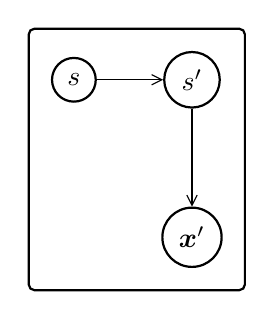
\begin{tikzpicture}
    \tikzstyle{enode} = [thick, draw=black, circle, align=center]
    \tikzstyle{cnode} = [thick, draw=black, circle, align=center, inner sep = 0.3pt]
    \tikzstyle{nnode} = [thick, rectangle, rounded corners = 2pt,minimum size = 0.8cm,draw,inner sep = 8pt]
    \node[enode] (s) at (-1.5,2) {${s}$};
    \node[enode] (x) at (0,0){$\bm{x}^{\prime}$};
    \node[enode] (sp) at (0,2){${s}^{\prime}$};
    \node[nnode, fit=(x)(sp)(s)] (box) {};
    % \node[] at (-1.8,-0.4) {$\abs{\Dd}$};
    
    \draw[->] (s) to (sp);
    \draw[->] (sp) to (x);

  \end{tikzpicture}
  \caption{The template model of HMM.}\label{chpt7:fig:hmm-template}
\end{subfigure}
\hspace{5pt}
\begin{subfigure}{0.45\textwidth}
  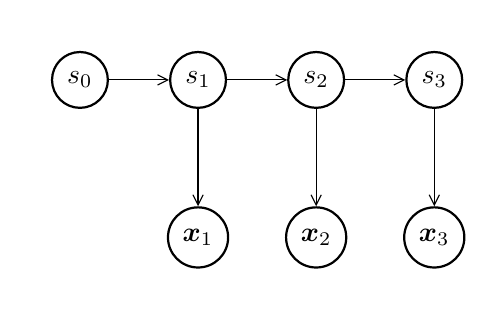
\begin{tikzpicture}
    \tikzstyle{enode} = [thick, draw=black, circle, align=center]
    \tikzstyle{cnode} = [thick, draw=black, circle, align=center, inner sep = 0.3pt]
    \tikzstyle{nnode} = [thick, rectangle, rounded corners = 2pt,minimum size = 0.8cm,draw,inner sep = 8pt]
    \node[enode] (s0) at (0,2) {${s}_0$};
    \node[enode] (s1) at (1.5,2){${s}_1$};
    \node[enode] (s2) at (3,2){${s}_2$};
    \node[enode] (s3) at (4.5,2){${s}_3$};
    
    \node[enode] (x1) at (1.5,0){$\bm{x}_1$};
    \node[enode] (x2) at (3,0){$\bm{x}_2$};
    \node[enode] (x3) at (4.5,0){$\bm{x}_3$};
    \node[nnode, draw=white, fit=(s0)(s1)(x1)] (box) {};
    
    \draw[->] (s0) to (s1);
    \draw[->] (s1) to (s2);
    \draw[->] (s2) to (s3);

    \draw[->] (s1) to (x1);
    \draw[->] (s2) to (x2);
    \draw[->] (s3) to (x3);
    
  \end{tikzpicture}
  % \vskip 10pt
  \caption{The unrolled HMM instance to time $t=3$.}\label{chpt7:fig:hmm-instance}
\end{subfigure}
\caption{From HMM template to instance.}\label{chpt7:fig:hmm-inituition}
\end{figure}

We first illustrate the concepts of Markov assumption and \textit{template} with an example before giving the definition of HMM. As shown in Figure~\ref{chpt7:fig:hmm-template}, the plate denotes the template within which the generic variables and their dependencies (template variables and factors) are represented. As a dynamic system evolves with time, the hidden variable $s$ and observed variable $\bm{x}$ can be instantiated for each time slice $t$, along with their dependencies. Figure~\ref{chpt7:fig:hmm-instance} is an instantiated example up to $t=3$ from the generic template. The Markov assumption is embedded in the HMM instances from the template since Markov independence is fulfilled no matter how long the system evolves. More importantly, the conditional probabilities $p(s_{t+1}|s_{t}),~\forall~t$, instantiated from template factors (defined with the directed edge $s\rightarrow s^{\prime}$ in Figure~\ref{chpt7:fig:hmm-template}), share the same parameterization. Similarly, the probabilities $p(\bm{x}_{t}|s_{t}),~\forall~t$ share parameterization with the template factor defined with edge $s^{\prime}\rightarrow \bm{x}^{\prime}$. This definition circumvents the exponential growth of parameterization. 

With the intuition from Figure~\ref{chpt7:fig:hmm-inituition}, we now define the HMM with its parameterization. A HMM $\bm{H}$ defined in a hypothesis space $\Hh$, i.e. $\bm{H} \in \Hh$, is capable to model a time-span signal $\ubar{\bm{x}} = \left[ \bm{x}_1, \cdots, \bm{x}_T\right]^{\intercal}$, where $\bm{x}_t\in \RR^{N}$ is the $N$-dimensional signal at time $t$, $[\cdot]^{\intercal}$ denotes transpose, and $T$ denotes the time length\footnote{The length for  sequential data varies.}. We define the hypothesis set of HMM as $\Hh := \{\bm{H} | \bm{H}=\{\Ss, \bm{q}, \bm{A}, p(\bm{x}|{s}; \bm{\Phi}_{s})\}\}$, where
\begin{itemize}
\item $\Ss$ is the set of hidden states of $\bm{H}$.
\item $\bm{q} = \left[ q_1, q_2, \cdots, q_{|\Ss|}\right]^\intercal$ is the initial state distribution of $\bm{H}$ with $|\Ss|$ as cardinality of $\Ss$. For $i \in \Ss$, $q_i = p(s_{1}=i;\bm{H})$. We use $s_t$ to denote the state $s$ at time $t$.
\item $\bm{A}$ matrix of size $|\Ss| \times |\Ss|$ is the transition matrix of states in $\bm{H}$. That is, $\forall i, j \in \Ss$,  $\bm{A}_{i,j} = p(s_{t+1}=j|s_{t}=i; \bm{H})$.
\item For a given hidden state $s$, the density function of the observable signal is $p({\bm{x}}|{s};\bm{\Phi}_{s})$, where $\bm{\Phi}_{s}$ is the parameter set that defines this probabilistic model. Denote $\bm{\Phi} = \left\{ \bm{\Phi}_{s}| s \in \Ss \right\}$.
\end{itemize}


\begin{figure}[!t]
  \centering
  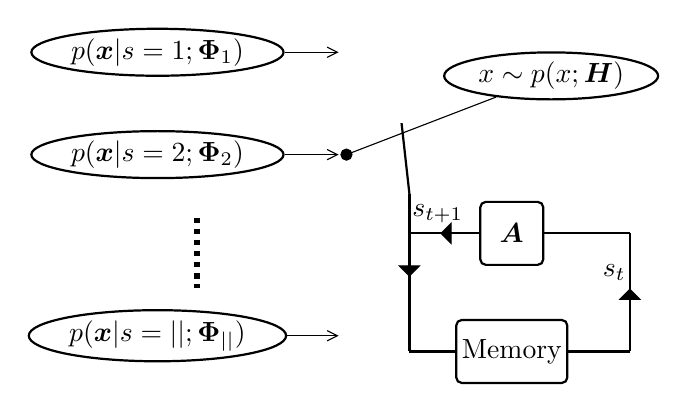
\begin{tikzpicture}
    \tikzstyle{enode} = [thick, draw=black, ellipse, inner sep = 1pt,  align=center]
    \tikzstyle{nnode} = [thick, rectangle, rounded corners = 2pt,minimum size = 0.8cm,draw,inner sep = 2pt]
    \node[enode] (g1) at (-0.5,1.8) {$p(\bm{x}| s=1; \bm{\Phi}_{1})$};
    \node[enode] (g2) at (-0.5,0.5) {$p(\bm{x}| s=2; \bm{\Phi}_{2})$};
    \node[enode] (gs) at (-0.5, -1.8) {$p(\bm{x}| s=|\Ss|; \bm{\Phi}_{|\Ss|})$};
    \node[enode] (x) at (4.5,1.5){$\ubm{x}\sim p(\ubm{x};\bm{H})$};

    \draw[dotted,line width=2pt] (0,-0.3) -- (0,-1.2);
    \filldraw[->] (1.9, 0.5)circle (2pt) --  (x) ;
    \draw[->] (g1) -- (1.8, 1.8);
    \draw[->] (g2) -- (1.8, 0.5);
    \draw[->] (gs) -- (1.8, -1.8);

    \begin{scope}[xshift=0.5cm, thick, every node/.style={sloped,allow upside down}]
      \node[nnode] (m) at (3.5,-2) {Memory};
      \node[nnode] (a) at (3.5,-0.5) {$\bm{A}$};

      \draw (2.1,0.9)-- (2.2, 0.);
      \draw (2.2,0.)-- node {\midarrow} (2.2,-2);
      \draw (2.2,-2)-- (m);
      \draw (m)-- (5, -2);
      \draw (5, -2)-- node {\midarrow} (5 ,-0.5);
      \draw (5, -0.5) -- (a);
      \draw (a)-- node {\midarrow} (2.2, -0.5);
      \node at (4.8, -1) {$s_{t}$};
      \node at (2.56, -0.25) {$s_{t+1}$};
    \end{scope}
  \end{tikzpicture}
  \caption{HMM model: a generative illustration.}\label{fig:hmm}
\end{figure}


A HMM for signal representation is illustrated in Figure~\ref{fig:hmm}. The model assumption is that different time instances of the signal $\ubar{\bm{x}}$ are generated by different signal sources where each signal source is associated with a hidden state of the HMM.
In the framework of HMM, at each time instance $t$, signal $\bm{x}_t$ is assumed to be generated by a distribution with density function $p(\bm{x}_t| s_t; \bm{\Phi}_{s_t})$, and $s_t$ is decided by the hidden Markov process. Putting these together gives us the probabilistic model $p(\ubm{x};\bm{H})$.

\begin{remark}
  The graphical model of an HMM is very similar to that of a CRF, especially linear-chain CRF. The straightforward difference between an HMM and a linear-chain CRF is the graphical model representation. An HMM is a pure directed probabilistic graphical model while there are both directed and undirected edges in a CRF. 

  In a nutshell, omitting observed variables and their variables, the remaining variables and their edges form an MRF in a CRF. This difference also affects the model training. An HMM is a generative model and models $p(\ubar{\bm{x}}, \ubar{{s}})$ jointly. Its training target is to maximize the joint probability. In contrast, a CRF models a conditional distribution $p(\ubar{{s}}|\ubar{\bm{x}})$ and is learned via discriminative training. CRFs are popular applied to structure prediction such as natural language processing, computer vision, bioinformatics, etc.
See \cite{charles2012crf} for a more detailed discussion on the difference between them.
\end{remark}

\section{Generator-mixed HMM}

In this section, we introduce a generator-mixed hidden Markov model (GenHMM). The highlight of GenHMM is that its state probability distributions are induced by normalizing flows for flexible dependency modeling between hidden states and observed signals. The learning of GenHMM is discussed here at a high level while the detailed solutions would be presented in Section~\ref{chpt7:sec:practical-sol-genhmm}.

\subsection{Generators of GenHMM}

\begin{figure}[!t]
  \centering
  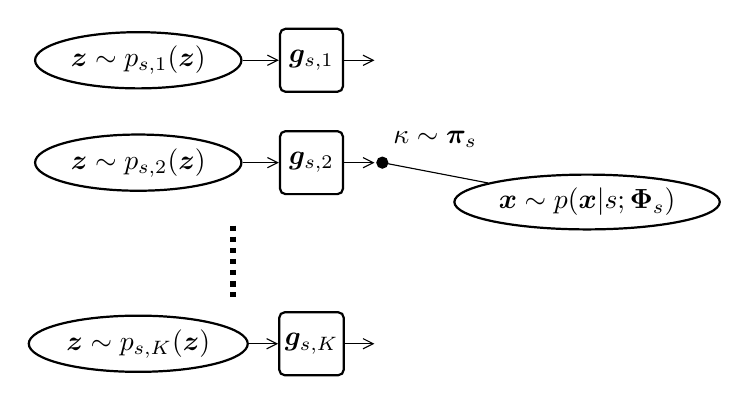
\begin{tikzpicture}
    \tikzstyle{enode} = [thick, draw=black, ellipse, inner sep = 2pt,  align=center]
    \tikzstyle{nnode} = [thick, rectangle, rounded corners = 2pt,minimum size = 0.8cm,draw,inner sep = 2pt]
    \node[enode] (z1) at (-1.2,1.8) {$\bm{z}\sim p_{s,1}(\bm{z})$};
    \node[nnode] (g1) at (1,1.8) {$\bm{g}_{s,1}$};
    \node[enode] (z2) at (-1.2,0.5){$\bm{z}\sim p_{s,2}(\bm{z})$};
    \node[nnode] (g2) at (1,0.5) {$\bm{g}_{s,2}$};
    \node[enode] (zK) at (-1.2,-1.8) {$\bm{z}\sim p_{s,K}(\bm{z})$};
    \node[nnode] (gs) at (1, -1.8) {$\bm{g}_{s,K}$};
    \node[enode] (x) at (4.5,0){$\bm{x}\sim p(\bm{x}| s; \bm{\Phi}_{s})$};

    \draw[dotted,line width=2pt] (0,-0.3) -- (0,-1.2);
    \filldraw[->] (1.9, 0.5)circle (2pt) --  node[above=0.2]{${\kappa}\sim \bm{\pi}_{s}$} (x)  ;
    \draw[->] (z1) -- (g1);
    \draw[->] (g1) -- (1.8, 1.8);

    \draw[->] (z2) -- (g2);
    \draw[->] (g2) -- (1.8, 0.5);

    \draw[->] (zK) -- (gs);
    \draw[->] (gs) -- (1.8, -1.8);
  \end{tikzpicture}
  \caption{Template factor of GenHMM: conditional probabilistic model of observed variable $\bm{x}$ given hidden state $s$.}
  \label{fig:gen-mix}
\end{figure}

In this section, we introduce normalizing flows to each state probabilistic models of our GenHMM, which models the conditional probability of observation given a hidden state.
Recall that $\bm{x}\in\mathbb{R}^N$. The subscript is omitted when it does not cause ambiguity.
The probabilistic model of GenHMM for each hidden state is a mixture of $K$ flow generators that are implemented by neural networks, where $K$ is a positive integer.
The probabilistic model of a state $s\in\Ss$ is then given by
\begin{equation}\label{eq:state-prob-model}
  p(\bm{x}| s; \bm{\Phi}_{s}) = \sum_{\kappa=1}^{K}\pi_{s, \kappa} p(\bm{x}| s, \kappa; \bm{\theta}_{s, \kappa}),
\end{equation}
where $\kappa$ is a random variable following a categorical distribution, with probability $\pi_{s, \kappa} = p(\kappa | s; \bm{H})$.
Naturally $\sum_{\kappa = 1}^{K} \pi_{s, \kappa}= 1$. Denote $\bm{\pi}_{s} = [\pi_{s,1}, \pi_{s,2}, \cdots, \pi_{s,K}]^{\intercal}$. 
In \eqref{eq:state-prob-model}, $p(\bm{x}| s, \kappa; \bm{\theta}_{s, \kappa})$ is further defined as the induced distribution by a generator $\bm{g}_{s,\kappa}: \RR^{N}\rightarrow\RR^{N}$, such that $\bm{x}=\bm{g}_{s, \kappa}(\bm{z})$, where $\bm{z}$ is a latent variable following a distribution with density function $p_{s,\kappa}(\bm{z})$. Generator $\bm{g}_{s,\kappa}$ is parameterized by $\bm{\theta}_{s, \kappa}$. Let us denote the collection of the parameter sets of generators for state $s$ as $\bm{\theta}_s = \left\{ \bm{\theta}_{s, \kappa}| \kappa = 1, 2, \cdots, K \right\}$. For a flow generator $\bm{g}_{s, \kappa}$, we have
\begin{equation}\label{chpt7:eq:change-variable}
  p(\bm{x}| s, \kappa; \bm{\theta}_{s, \kappa}) = p_{s,\kappa}(\bm{z})\bigg| \det\left( \pd{\bm{g}_{s,\kappa}(\bm{z})}{\bm{z}} \right)\bigg|^{-1}, ~\mathrm{with}~ \bm{x}=\bm{g}_{s,\kappa}(\bm{z}),
\end{equation}
which is discussed in detail in Section~\ref{chpt6:sec:flow}.

The signal generating process of the probability distribution for a state $s$ of GenHMM is shown in Figure~\ref{fig:gen-mix}, in which the generator identity is up to the random variable $\kappa$. This serves as the template factor in instantiating the chain of a HMM. The normalizing flows with neural network realizations of their coupling mapping \eqref{chpt6:eq-gl-coupling} offer a richer probability density function space and higher model expressivity. This naturally enriches the feasible space $\Hh$. Putting these together with the typical Markov assumption, the template model of GenHMM is illustrated in Figure~\ref{chpt7:fig:tenhmm-template}. As a dynamic system evolves, we can instantiate from the template model in Figure~\ref{chpt7:fig:tenhmm-template} to create the dynamic chain of graphical model representation. Similar to a typical HMM, the parameterization of GenHMM can be fully explained by its template model and does not grow exponentially when instantiating over the evolving system.

\subsection{Learning with the EM framework}

Assume the sequential signal $\ubm{x}$ follows the true distribution $p^{\ast}(\ubm{x})$, which is unknown. We would like to use GenHMM to model this distribution. Alternatively, we are addressing
\begin{equation}
  \umin{\bm{H}\in \Hh} \mathrm{KL}({p^{\ast}}(\ubm{x})\| p(\ubm{x};\bm{H})).
\end{equation}
For practical consideration, we only have access to the samples of $p^{\ast}(\ubm{x})$, i.e. a dataset consisting of samples drawn from this distribution. For the given dataset, we denote its empirical distribution by $\hat{p}(\ubm{x}) = \frac{1}{R}\sum_{r=1}^{R} \delta_{\ubmr{x}{r}}(\ubm{x})$, where $R$ denotes the total number of sequential samples and superscipt $(\cdot)^{r}$ denotes the index of $r$-th sequential signal. Similar to the analysis in Section~\ref{chpt2:sec:learning-principles}, the KL divergence minimization problem can be reduced to a likelihood maximization problem
\begin{equation}\label{eq:ml-of-hmm}
  \uargmax{\bm{H} \in \Hh} \frac{1}{R}\sum_{r=1}^{R}\log\,p(\ubmr{x}{r}; \bm{H}).
\end{equation}

\begin{figure}[tp!]
  \centering
  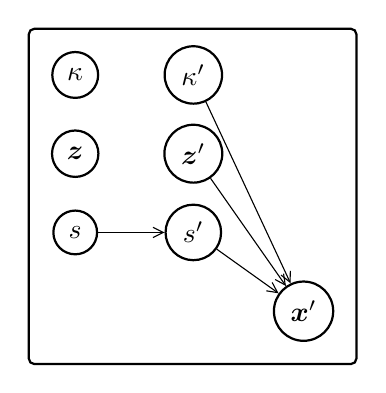
\begin{tikzpicture}
    \tikzstyle{enode} = [thick, draw=black, circle, align=center]
    \tikzstyle{cnode} = [thick, draw=black, circle, align=center, inner sep = 0.3pt]
    \tikzstyle{nnode} = [thick, rectangle, rounded corners = 2pt,minimum size = 0.8cm,draw,inner sep = 8pt]
    \node[enode] (s) at (-1.5,-1) {${s}$};
    \node[enode] (k) at (-1.5,1) {${\kappa}$};
    \node[enode] (z) at (-1.5,0) {$\bm{z}$};
    
    \node[enode] (sp) at (0,-1){${s}^{\prime}$};
    \node[enode] (kp) at (0,1){${\kappa}^{\prime}$};
    \node[enode] (zp) at (0,0){$\bm{z}^{\prime}$};
    
    \node[enode] (x) at (1.4,-2){$\bm{x}^{\prime}$};
    
    \node[nnode, fit=(x)(z)(k)(s)] (box) {};
    % \node[] at (-1.8,-0.4) {$\abs{\Dd}$};
    
    \draw[->] (s) to (sp);
    \draw[->] (sp) to (x);
    \draw[->] (zp) to (x);
    \draw[->] (kp) to (x);
  \end{tikzpicture}
  \caption{The template model of GenHMM.}\label{chpt7:fig:tenhmm-template}
\end{figure}
For the likelihood maximization, the first problem that we need to address is how to deal with the hidden sequential variables of model $\bm{H}$, namely $\ubm{s}=[ \bm{s}_1, \bm{s}_2, \cdots, \bm{s}_T ]^{\intercal}$ and $\ubm{\kappa} = [\bm{\kappa}_1, \bm{\kappa}_2, \cdots, \bm{\kappa}_T]^{\intercal}$. For a sequentially observable variable $\ubm{x}$, $\ubm{s}$ is the hidden state sequence corresponding to $\ubm{x}$, and $\ubm{\kappa}$ is the hidden variable sequence representing the generator identity sequence that actually generates $\ubm{x}$. Note that for a sequentially observable $\ubm{x}$, there is also a sequential $\ubm{z}$ brought by flows. But the mapping between $\bm{x}$ and $\bm{z}$ is deterministic for fixed $p_{s,\kappa}(\bm{z})$ when the corresponding $\bm{s}$ and ${\kappa}$ are given, which is defined by $\bm{g}_{s, \kappa}$.

Since directly maximizing likelihood is not an option for our problem in \eqref{eq:ml-of-hmm}, we address this problem with the EM framework, similar to the way we dealt with hidden variable in Section~\ref{chpt6:sec:generator-mix-em}. This divides our problem into  two iterative steps: i) using the joint posterior of hidden variable sequences $\ubm{s}$ and $\ubm{\kappa}$ to obtain an ``expected likelihood'' of the observable variable sequence $\ubm{x}$, i.e. the E-step; ii) maximizing the expected likelihood with regard to the model $\bm{H}$, i.e. the M-step. Assume model $\bm{H}$ is at a configuration of $\bm{H}^{\mathrm{old}}$, we formulate these two steps as follows.
\begin{itemize}
\item E-step: % the posterior probability of $\ubm{s}$:
  % \begin{equation}
  %   p(\ubm{s}|\ubm{x})
  % \end{equation}
  the expected likelihood function
  \begin{equation}\label{eq:em-q-funciton}
    \Qq(\bm{H}; \bm{H}^{\mathrm{old}}) = \EE_{\hat{p}(\ubm{x}),p(\ubm{s},\ubm{\kappa}| \ubm{x}; \bm{H}^{\mathrm{old}})}\left[ \log\,p(\ubm{x}, \ubm{s}, \ubm{\kappa}; \bm{H})\right],
  \end{equation}
  where $\EE_{\hat{p}(\ubm{x}),p(\ubm{s},\ubm{\kappa}| \ubm{x}; \bm{H}^{\mathrm{old}})}\left[ \cdot\right]$ denotes the expectation operator by distribution $\hat{p}(\ubm{x})$ and $p(\ubm{s},\ubm{\kappa}| \ubm{x}; \bm{H}^{\mathrm{old}})$.
\item M-step: the maximization step
  \begin{equation}\label{eq:em-m-opt}
    \umax{\bm{H}} \Qq(\bm{H}; \bm{H}^{\mathrm{old}}).
  \end{equation}
\end{itemize}


The problem \eqref{eq:em-m-opt} can be reformulated as
\begin{align}\label{eq:m-step-subs}
  \umax{\bm{H}} \Qq(\bm{H}; \bm{H}^{\mathrm{old}})
  =\umax{\bm{q}}\Qq(\bm{q}; \bm{H}^{\mathrm{old}}) + \umax{\bm{A}}\Qq(\bm{A}; \bm{H}^{\mathrm{old}}) 
     + \umax{\bm{\Phi}}\Qq(\bm{\Phi}; \bm{H}^{\mathrm{old}}),
\end{align}
where the decomposed optimization problems are
\begin{align}
  \Qq(\bm{q}; \bm{H}^{\mathrm{old}}) 
  % &=\EE_{\hat{p}(\ubm{x}),p(\ubm{s},\ubm{\kappa}| \ubm{x}; \bm{H}^{\mathrm{old}})} \left[ \log\,p({s}_{1})  \right] \nonumber\\
    &= \EE_{\hat{p}(\ubm{x}),p(\ubm{s}| \ubm{x}; \bm{H}^{\mathrm{old}})} \left[ \log\,p({s}_{1};\bm{H})  \right], \label{eq:init-distribution-update}\\
  \Qq(\bm{A}; \bm{H}^{\mathrm{old}}) &=\EE_{\hat{p}(\ubm{x}),p(\ubm{s}| \ubm{x}; \bm{H}^{\mathrm{old}})}\hspace{-0.1cm}\left[ \sum_{t=1}^{T-1}\log\,p({s}_{t+1}|{s}_{t}; \bm{H}) \right], \label{eq:transition-update}\\
  \Qq(\bm{\Phi}; \bm{H}^{\mathrm{old}}) &= \EE_{\hat{p}(\ubm{x}),p(\ubm{s},\ubm{\kappa}| \ubm{x}; \bm{H}^{\mathrm{old}})} \left[ \log\,p(\ubm{x}, \ubm{\kappa}| \ubm{s}; \bm{H}) \right]. \label{eq:generative-model-update}
\end{align}

We can see that the solution of $\bm{H}$ depends on the posterior probability $p(\ubm{s}| \ubm{x}; \bm{H})$.

\begin{remark}[On posterior]\label{chpt7:rmk:posterior}
  Although the principle here in dealing with the hidden variables is similar to that in Section~\ref{chpt6:sec:generator-mix-em}, new issues arise for dynamic systems. Due to the presence of incomplete observations (hidden variables), we need to 'complete' the missing information by evaluating the posteriors of hidden variables for each partial observation $\bm{x}_t$. In GenHMM, for each $\ubm{x}$, there are missing hidden sequences ($\ubm{s}$, $\ubm{\kappa}$). Although the evaluation of the posterior according to Bayes theorem is straightforward, the computational complexity of $p(\ubm{s}| \ubm{x}; \bm{H})$ grows exponentially with the length of $\ubm{s}$. Therefore, we employ forward-backward algorithm \cite{Bishop:2006:PRM:1162264}, i.e. a message passing algorithm for chains which computes exact marginal probabilities, to do the posterior computation efficiently. The forward-backward algorithm can be recovered from the generic message passing rule \eqref{chpt2:eq:loopy-bp} in Section~\ref{chpt2:sec:inference-mp}.
As we will detail in the next section, what is needed to formulate the problem, are actually the $p(s| \ubm{x}; \bm{H})$ and $p(s, \kappa| \ubm{x}; \bm{H})$. For the joint posterior $p(s, \kappa| \ubm{x}; \bm{H})$, it can be computed by the Bayes rule when posterior of hidden state is available.
\end{remark}
\begin{remark}[Connection to other methods or models]\label{chpt7:rmk:connections}
  The forward-background algorithm mentioned in Remark~\ref{chpt7:rmk:posterior} does exact inference to posteriors, i.e. the exact computation of posterior probabilities. At times, the posterior inference is addressed by approximate inference. For instance, it might be due to the modeling of a dynamic system that does not allow exact inference. \cite{yuan2007thesis} applies expectation propagation \cite{Minka:2001:EPA:647235.720257} to non-linear dynamic models with continuous hidden states.
  
  The considered hidden states are discrete in GenHMM. For linear dynamic models with continuous hidden states, the best-known approach is the Kalman filter \cite{kalman1960} and smoothing \cite{rauch1965}. To generalize the problem into non-linear dynamic models, which is practical consideration since many real-world problems are indeed non-linear, known classical methods such as extended Kalman filter \cite{ljung1979} and unscented Kalman filter \cite{wan2000unscented} are applicable. Further exploration in recent literature also considered more flexible models such as neural networks in dynamic models. For instance, \cite{wallach2019hybrid} combined the inference process of Kalman filter and graph neural network in pursuit of more flexible non-linear dynamic models, and \cite{kim2019variational} proposed hierarchical hidden state space to model and infer hidden structures with multi-layer perceptrons.
\end{remark}

With such a solution framework ready, we detail the practical learning algorithm for GenHMM with normalizing flows embedded in next section.

\section{Practical Solution to GenHMM}
\label{chpt7:sec:practical-sol-genhmm}
In this section, we detail the solution for realizing and learning GenHMM. The convergence of GenHMM is also discussed in this section.


\subsection{Realizing $\bm{g}_{s,\kappa}$ by a Flow Model}
Each generator $\bm{g}_{s,\kappa}$ is realized as a feed-forward neural netowrk.
We define generator $\bm{g}_{s,\kappa}$ as a $L$-layer flow model and formulate its mapping by layer-wise concatenation
\begin{equation}
\bm{g}_{s,\kappa}=\bm{g}_{s,\kappa}^{[L]}\circ \bm{g}_{s,\kappa}^{[L-1]}\circ \cdots \circ \bm{g}_{s,\kappa}^{[1]},
\end{equation}
where superscript $[l]$ denotes the layer index and $\circ$ denotes mapping concatenation. As detailed in Section~\ref{chpt6:sec:flow}, generator $\bm{g}_{s,\kappa}$ is invertible, and we denote its inverse mapping as $\bm{f}_{s,\kappa}=\bm{g}_{s,\kappa}^{-1}$. Then \eqref{chpt7:eq:change-variable} can be rewritten as
\begin{equation}\label{chpt7:eq:change-variable-flow}
  \log{p(\bm{x}| s, \kappa; \bm{\theta}_{s, \kappa})} = \log{p_{s,\kappa}(\bm{f}_{s, \kappa}(\bm{x}))} + \log{\bigg| \det\left( \pd{\bm{f}_{s,\kappa}(\bm{x})}{\bm{z}} \right)\bigg|},
\end{equation}
where $\bm{z}=\bm{f}_{s,\kappa}(\bm{x})$.
By decomposing the flow model into layer-wise mappings, the Jacobian matrix determinant becomes
\begin{equation}\label{eq:cat-jacobian}
  \begin{array}{rl}
    \mathrm{det}(\nabla{\bm{f}_{s,\kappa}}) = \prod_{l=1}^L \det (\nabla{\bm{f}_{s,\kappa}^{[l]}}),
  \end{array}
\end{equation}
where $\nabla{\bm{f}_{s,\kappa}^{[l]}}$ is the Jacobian of the mapping from the $l$-th layer to the $(l-1)$-th layer, i.e., the inverse transformation.
Then \eqref{chpt7:eq:change-variable-flow} can be further rewritten as
\begin{equation}\label{chpt7:eq:change-variable-flow-layer}
  \log{p(\bm{x}| s, \kappa; \bm{\theta}_{s, \kappa})} = \log{p_{s,\kappa}(\bm{f}_{s, \kappa}(\bm{x}))} + \sum_{l=1}^{L}\log{\bigg| \det\left(\nabla{\bm{f}_{s,\kappa}^{[l]}}\right)\bigg|}.
\end{equation}


\subsection{Learning of GenHMM}\label{subsec:optmGenHMM}
In this section, we address the problem of learning GenHMM.
\subsubsection{Learning of Generators and Their Weights}
Learning of a mixture of generators is actually equivalent to solving the problem in \eqref{eq:generative-model-update}, which can be further divided into two subproblems: i) generator learning and ii) mixture weight learning for the generators. Let us define some notations:
$\bm{\Pi} = \left\{  \bm{\pi}_{s}| s\in \Ss \right\}$, $\bm{\Theta}=\left\{ \bm{\theta}_s| s\in \Ss \right\}$. 
Then the problem in \eqref{eq:generative-model-update} becomes
\begin{align}\label{eq:sub-gm}
  &\umax{\bm{\Phi}} \Qq(\bm{\Phi}; \bm{H}^{\mathrm{old}}) = \umax{\bm{\Pi}} \Qq(\bm{\Pi}; \bm{H}^{\mathrm{old}}) + \umax{\bm{\Theta}} \Qq(\bm{\Theta}; \bm{H}^{\mathrm{old}}),
\end{align}
where
\begin{align}
  \Qq(\bm{\Pi}; \bm{H}^{\mathrm{old}})  &=\EE_{\hat{p}(\ubm{x}),p(\ubm{s},\ubm{\kappa}| \ubm{x}; \bm{H}^{\mathrm{old}})}\left[  \log\,p(\ubm{\kappa}| \ubm{s}; \bm{H})\right], \\
  \Qq(\bm{\Theta}; \bm{H}^{\mathrm{old}}) &=\EE_{\hat{p}(\ubm{x}),p(\ubm{s},\ubm{\kappa}| \ubm{x}; \bm{H}^{\mathrm{old}})}\left[  \log\,p(\ubm{x}| \ubm{s},\ubm{\kappa}; \bm{H})\right].
\end{align}

We firstly address the generator learning problem, i.e. $\umax{\bm{\Theta}} \Qq(\bm{\Theta}; \bm{H}^{\mathrm{old}})$. This boils down to maximizing the cost function of neural networks that can be formulated as
\begin{align}\label{eq:obj-q-gen-mix-log}
  &\Qq(\bm{\Theta}; \bm{H}^{\mathrm{old}}) \nonumber \\
  = &\frac{1}{R}\sum_{r=1}^{R}\sum_{\ubmr{s}{r}}\sum_{\ubmr{\kappa}{r}}{p(\ubmr{s}{r}, \ubmr{\kappa}{r}| \ubmr{x}{r}; \bm{H}^{\mathrm{old}})} \sum_{t=1}^{{T}^{r}}\log\,p(\bmtr{x}{t}{r} | \smtr{s}{t}{r}, \smtr{\kappa}{t}{r}; \bm{H}) \nonumber \\
  =& \frac{1}{R}\sum_{r=1}^{R} \sum_{t=1}^{{T}^{r}} \sum_{\smtr{s}{t}{r}=1}^{|\Ss|}  \sum_{\smtr{\kappa}{t}{r}=1}^{K}p(\smtr{s}{t}{r}| \ubmr{x}{r}; \bm{H}^{\mathrm{old}})p(\smtr{\kappa}{t}{r}|\smtr{s}{t}{r}, \ubmr{x}{r}; \bm{H}^{\mathrm{old}})  \log\, p(\bmtr{x}{t}{r} | \smtr{s}{t}{r}, \smtr{\kappa}{t}{r}; \bm{H}), 
\end{align}
where $T^r$ is the length of the $r$-th sequential data. In \eqref{eq:obj-q-gen-mix-log}, the state posterior $p(s_t| \ubm{x}, \bm{H}^{\mathrm{old}})$ is computed by forward-backward algorithm. The posterior of $\kappa$ is
\begin{align}\label{eq:kappa-posterior}
  p(\kappa| s, \ubm{x}; \bm{H}^{\mathrm{old}})
  &=  \frac{p(\kappa, \ubm{x}| s; \bm{H}^{\mathrm{old}})}{p(\ubm{x}| s,\bm{H}^{\mathrm{old}})} \nonumber \\
  & = \frac{\pi_{s, \kappa}^{\mathrm{old}} p(\bm{x}| s, \kappa, \bm{H}^{\mathrm{old}})}{\sum_{\kappa=1}^{K}  \pi_{s, \kappa}^{\mathrm{old}} p(\bm{x}| s, \kappa,\bm{H}^{\mathrm{old}})},
\end{align}
where the last equation is due to the fact that $\bm{x}_t$ among sequence $\ubm{x}$ is conditional independent of $\bm{x}_{t^{\prime}}$ given $s_t$ and $\kappa_t$ for $t\neq t^{\prime}$. 

By substituting \eqref{chpt7:eq:change-variable-flow-layer} into \eqref{eq:obj-q-gen-mix-log}, we have the cost function for the neural networks as
\begin{align}\label{eq:obj-q-gen-mix}
  &\Qq(\bm{\Theta}; \bm{H}^{\mathrm{old}}) \nonumber \\
  =& \frac{1}{R}\hspace{-3pt}\sum_{r=1}^{R}\hspace{-3pt} \sum_{t=1}^{{T}^{r}}\hspace{-3pt} \sum_{\smtr{s}{t}{r}=1}^{|\Ss|} \hspace{-3pt} \sum_{\smtr{\kappa}{t}{r}=1}^{K}p(\smtr{s}{t}{r}| \ubmr{x}{r}; \bm{H}^{\mathrm{old}})p(\smtr{\kappa}{t}{r}|\smtr{s}{t}{r}, \ubmr{x}{r}; \bm{H}^{\mathrm{old}}) \nonumber\\
  &\left[ \log\, p_{\smtr{s}{t}{r}, \smtr{\kappa}{t}{r}}(\bm{f}_{\smtr{s}{t}{r}, \smtr{\kappa}{t}{r}}(\bmtr{x}{t}{r})) + \sum_{l=1}^{L}\log\,| \det (\nabla{\bm{f}_{s,\kappa}^{[l]}})|\right].
\end{align}
The generators of GenHMM simply use standard Gaussian distribution for latent variables $\bm{z} \sim p_{s,\kappa}(\bm{z})$. Since the training dataset can be too large to do whole-dataset iterations, batch-size stochastic gradient descent can be used to maximize $\Qq(\bm{\Theta; \bm{H}^{\mathrm{old}}})$ with regard to parameters of generators.

In what follows we address the problem $\max_{\bm{\Pi}} \Qq(\bm{\Pi}; \bm{H}^{\mathrm{old}})$ in our generative model learning. The conditional distribution of hidden variable $\kappa$, $\pi_{s, \kappa} = p(\kappa | s; \bm{H})$, is obtained by solving the following problem
\begin{align}\label{opm:pi}
  \pi_{s, \kappa} & = \uargmax{\pi_{s, \kappa}} \Qq(\bm{\Pi}; \bm{H}^{\mathrm{old}}) \\ \nonumber
                  & s.t. \, \sum_{\kappa=1}^{K} \pi_{s, \kappa}= 1, \forall s = 1, 2, \cdots, |\Ss|. 
\end{align}

To solve problem \eqref{opm:pi}, we formulate its Lagrange function as
\begin{equation}
  \Ff = \Qq(\bm{\Pi}; \bm{H}^{\mathrm{old}}) + \sum_{s=1}^{|\Ss|} \lambda_s\left( 1-  \sum_{\kappa=1}^{K}\pi_{s, \kappa}  \right).
\end{equation}
Solving $\pd{\Ff}{\pi_{s, \kappa}} = 0$ gives
\begin{equation}
  \pi_{s,\kappa} = \frac{1}{\lambda_s}\sum_{r=1}^{R} \sum_{t=1}^{{T}^{r}} p(\smtr{s}{t}{r}=s, \smtr{\kappa}{t}{r} =\kappa| \ubmr{x}{r}; \bm{H}^{\mathrm{old}}).
\end{equation}
With condition $\sum_{\kappa=1}^{K} \pi_{s, \kappa}= 1, \forall s = 1, 2, \cdots, |\Ss|$, we have
\begin{equation}
  \lambda_s = \sum_{\kappa=1}^{K}\sum_{r=1}^{R} \sum_{t=1}^{{T}^{r}} p(\smtr{s}{t}{r}=s, \smtr{\kappa}{t}{r} =\kappa | \ubmr{x}{r}; \bm{H}^{\mathrm{old}}).
\end{equation}
Then the solution to \eqref{opm:pi} is
\begin{equation}\label{eq:mix-latent-parameter-solution}
  \pi_{s, \kappa} = \frac{\sum_{r=1}^{R} \sum_{t=1}^{{T}^{r}} p(\smtr{s}{t}{r} =s, \smtr{\kappa}{t}{r}=\kappa | \ubmr{x}{r}; \bm{H}^{\mathrm{old}}) }{\sum_{k =1}^{K}\sum_{r=1}^{R} \sum_{t=1}^{{T}^{r}} p(\smtr{s}{t}{r} =s, \smtr{\kappa}{t}{r}=k | \ubmr{x}{r}; \bm{H}^{\mathrm{old}}) },
\end{equation}
where
\begin{equation}
  p(s, \kappa | \ubm{x}; \bm{H}^{\mathrm{old}}) = p(s| \ubm{x}; \bm{H}^{\mathrm{old}}) p(\kappa | s, \ubm{x}; \bm{H}^{\mathrm{old}}).
\end{equation}
Here $p(s| \ubm{x}; \bm{H}^{\mathrm{old}})$ can be computed by forward-backward algorithm, while $p(\kappa | s, \ubm{x}; \bm{H}^{\mathrm{old}})$ is given by \eqref{eq:kappa-posterior}.


With the generator learning obtained, it remains to solve the initial distribution update and transition matrix update of HMM in GenHMM, i.e. the problem \eqref{eq:init-distribution-update} and \eqref{eq:transition-update}. These two problems are basically two constrained optimization problems. The solutions to them are available in the literature \cite{Bishop:2006:PRM:1162264}. But to keep the learning algorithm for GenHMM complete, we give the update rules for $\bm{q}$ and $\bm{A}$ as follows.

\subsubsection{Initial Probability Update}
The problem in \eqref{eq:init-distribution-update} can be reformulated as
\begin{align}
  &\Qq(\bm{q}; \bm{H}^{\mathrm{old}}) \nonumber \\
  =&\frac{1}{R} \sum_{r=1}^{R}\sum_{\ubmr{s}{r}} {p(\ubmr{s}{r}| \ubmr{x}{r}; \bm{H}^{\mathrm{old}})} \log\,p(\smtr{s}{1}{r};\bm{H}) \nonumber \\
  = & \frac{1}{R}\sum_{r=1}^{R}\sum_{\smtr{s}{1}{r}=1}^{|\Ss|}\sum_{\smtr{s}{2}{r}=1}^{|\Ss|}\cdots \sum_{\smtr{s}{T^{r}}{r}}^{{|\Ss|}} {p(\smtr{s}{1}{r}, \smtr{s}{2}{r}, \cdots, \smtr{s}{T^{r}}{r}| \ubmr{x}{r}; \bm{H}^{\mathrm{old}})} \log\,p(\smtr{s}{1}{r}) \nonumber\\
  =& \frac{1}{R}\sum_{r=1}^{R}\sum_{\smtr{s}{1}{r}=1}^{|\Ss|}{p(\smtr{s}{1}{r}| \ubmr{x}{r}; \bm{H}^{\mathrm{old}})} \log\,p(\smtr{s}{1}{r};\bm{H}).
\end{align}

$p(\smtr{s}{1}{r};\bm{H})$ is the probability of initial state of GenHMM for $r$-th sequential sample. Actually $q_i = p({s}_{1} =i;\bm{H}) $, $i= 1, 2, \cdots, |\Ss|$. Solution to the problem
\begin{align}
  \bm{q} \hspace{-0.1cm} = \hspace{-0.1cm} \uargmax{\bm{q}} \Qq(\bm{q}; \bm{H}^{\mathrm{old}}),\; \mathrm{s.t.} \sum_{i=1}^{ |\Ss| }q_i = 1, q_i \geq 0, \forall i.
\end{align}
is
\begin{equation}\label{eq:update-initial-state-prob}
  q_i = \frac{1}{R} \sum_{r=1}^{R} p(\smtr{s}{1}{r}=i | \ubmr{x}{r}; \bm{H}^{\mathrm{old}}), \forall\; i = 1, 2, \cdots, |\Ss|.
\end{equation}

\subsubsection{Transition Probability Update}
The problem \eqref{eq:transition-update} can be reformulated as
\begin{align}
  &\Qq(\bm{A}; \bm{H}^{\mathrm{old}})\nonumber \\
  % &= \sum_{r=1}^{R} \EE_{p(\ubmr{s}{r}| \ubmr{x}{r}; \bm{H}^{\mathrm{old}})} \left[\log\,\sum_{t=1}^{T^{(r)}-1}p(\smtr{s}{t+1}{r}|\smtr{s}{t}{r}; {A})\right] \nonumber\\
  =& \sum_{r=1}^{R} \sum_{\ubmr{s}{r}}{p(\ubmr{s}{r}| \ubmr{x}{r}; \bm{H}^{\mathrm{old}})} \sum_{t=1}^{T^{r}-1}\log\,p(\smtr{s}{t+1}{r}|\smtr{s}{t}{r}; \bm{H}) \nonumber \\
  =& \sum_{r=1}^{R} \hspace{-0.1cm}\sum_{t=1}^{T^{r}-1}\hspace{-0.1cm} \sum_{\smtr{s}{t}{r}=1}^{|\Ss|}\hspace{-0.05cm}\sum_{\smtr{s}{t+1}{r}=1}^{|\Ss|}\hspace{-0.2cm}{p(\smtr{s}{t}{r}, \smtr{s}{t+1}{r}| \ubmr{x}{r};\hspace{-0.05cm} \bm{H}^{\mathrm{old}})} \log\,p(\smtr{s}{t+1}{r}|\smtr{s}{t}{r}; \bm{H}).
\end{align}

Since $\bm{A}_{i, j}  = p(\smtr{s}{t+1}{r}=j|\smtr{s}{t}{r}=i; \bm{H})$ is the element of transition matrix $\bm{A}$, the solution to the problem
\begin{align}\label{eq:update-transition-prob}
  \bm{A} = &\uargmax{\bm{A}} \Qq(\bm{A}; \bm{H}^{\mathrm{old}}) \nonumber \\
  \mathrm{s.t.} &\hspace{0.2cm} \bm{A} \cdot \bm{1} = \bm{1}, \bm{A}_{i,j} \geq 0 \,\, \forall i,j,
\end{align}
is
\begin{equation}
  \bm{A}_{i,j} = \frac{\bar{\xi}_{i,j}}{\sum_{k = 1}^{|\Ss|} \bar{\xi}_{i,k}},
\end{equation}
where
\begin{equation}\label{eq:update-transition-solt}
  \bar{\xi}_{i,j} = \sum_{r= 1}^{R} \sum_{t= 1}^{T^{r}-1}{p(\smtr{s}{t}{r}=i, \smtr{s}{t+1}{r}=j| \ubmr{x}{r}; \bm{H}^{\mathrm{old}})}.
\end{equation}
\subsection{On Convergence of GenHMM}
In pursuit of representing a dataset by GenHMM,  we are interested if the learning solution discussed in Section~\ref{subsec:optmGenHMM} would converge. The properties of GenHMM's convergence are analyzed as follows.

\begin{proposition}\label{proposition1}
  Assume that parameter $\bm{\Theta} = \left\{ \bm{\theta}_{s,\kappa}| s\in \Ss, \kappa=1, 2, \cdots, K \right\}$ is in a compact set,  $\bm{f}_{s,\kappa}$ and  ${\nabla\bm{f}_{s,\kappa}}$ are continuous with regard to ${\bm\theta}_{s,\kappa}$ in GenHMM. Then GenHMM converges.
\end{proposition}

\begin{proof}
  We begin with the comparison of log-likelihood evaluated under $\bm{H}^{\mathrm{new}}$ and $\bm{H}^{\mathrm{old}}$. The log-likelihood of dataset given by $\hat{p}(\ubm{x})$ can be reformulated as
  \begin{align*}
    &\EE_{\hat{p}(\ubm{x})}\left[ \log\,p(\ubm{x};\bm{H}^{\mathrm{new}}) \right] \nonumber \\
    =& \EE_{\hat{p}(\ubm{x}),p(\ubm{s},\ubm{\kappa}| \ubm{x}; \bm{H}^{\mathrm{old}})}\left[ \log\,\frac{p(\ubm{x}, \ubm{s}, \ubm{\kappa}; \bm{H}^{\mathrm{new}})}{p(\ubm{s}, \ubm{\kappa}|\ubm{x}; \bm{H}^{\mathrm{old}})}\right]  \nonumber \\
    & +\EE_{\hat{p}(\ubm{x})}\left[ \mathrm{KL}(p(\ubm{s}, \ubm{\kappa}|\ubm{x}; \bm{H}^{\mathrm{old}})\|p(\ubm{s}, \ubm{\kappa}|\ubm{x}; \bm{H}^{\mathrm{new}})) \right],
  \end{align*}
  where the first term on the right hand side of the above inequality can be further written as
  \begin{align*}
    &\EE_{\hat{p}(\ubm{x}),p(\ubm{s},\ubm{\kappa}| \ubm{x}; \bm{H}^{\mathrm{old}})}\left[ \log\,\frac{p(\ubm{x}, \ubm{s}, \ubm{\kappa}; \bm{H}^{\mathrm{new}})}{p(\ubm{s}, \ubm{\kappa}|\ubm{x}; \bm{H}^{\mathrm{old}})}\right] \nonumber \\
    = &\Qq(\bm{H}^{\mathrm{new}}; \bm{H}^{\mathrm{old}}) + \EE_{\hat{p}(\ubm{x}),p(\ubm{s},\ubm{\kappa}| \ubm{x}; \bm{H}^{\mathrm{old}})}\left[p(\ubm{s}, \ubm{\kappa}|\ubm{x}; \bm{H}^{\mathrm{old}})\right].
  \end{align*}
  According to Section~\ref{subsec:optmGenHMM}, the optimization problems give
  \begin{align*}
    \Qq(\bm{q}^{\mathrm{new}}; \bm{H}^{\mathrm{old}}) &\geq \Qq(\bm{q}^{\mathrm{old}}; \bm{H}^{\mathrm{old}}),\nonumber \\
    \Qq(\bm{A}^{\mathrm{new}}; \bm{H}^{\mathrm{old}}) &\geq \Qq(\bm{A}^{\mathrm{old}}; \bm{H}^{\mathrm{old}}),\nonumber \\
    \Qq(\bm{\Pi}^{\mathrm{new}}; \bm{H}^{\mathrm{old}}) &\geq \Qq(\bm{\Pi}^{\mathrm{old}}; \bm{H}^{\mathrm{old}}), \nonumber \\
    \Qq(\bm{\Theta}^{\mathrm{new}}; \bm{H}^{\mathrm{old}}) &\geq \Qq(\bm{\Theta}^{\mathrm{old}}; \bm{H}^{\mathrm{old}}).
  \end{align*}
  % For the learning with regard to neural network parameter set $\bm{\Theta}$, as long as the lose function does not decrease during EM iterations, we would have
  Since
  \begin{align*}
    &\Qq(\bm{H}^{\mathrm{new}}; \bm{H}^{\mathrm{old}}) \nonumber \\
      = &\Qq(\bm{q}^{\mathrm{new}}; \bm{H}^{\mathrm{old}}) + \Qq(\bm{A}^{\mathrm{new}}; \bm{H}^{\mathrm{old}}) + \Qq(\bm{\Pi}^{\mathrm{new}}; \bm{H}^{\mathrm{old}})
                                                          + \Qq(\bm{\Theta}^{\mathrm{new}}; \bm{H}^{\mathrm{old}}),
  \end{align*}
  it gives
  \begin{equation*}
    \Qq(\bm{H}^{\mathrm{new}}; \bm{H}^{\mathrm{old}}) \geq \Qq(\bm{H}^{\mathrm{old}}; \bm{H}^{\mathrm{old}}).
  \end{equation*}
  With the above inequality, and the fact that $\EE_{\hat{p}(\ubm{x}),p(\ubm{s},\ubm{\kappa}| \ubm{x}; \bm{H}^{\mathrm{old}})}\left[p(\ubm{s}, \ubm{\kappa}|\ubm{x}; \bm{H}^{\mathrm{old}})\right]$ is independent of $\bm{H}^{\mathrm{new}}$, we have the inequality 
  \begin{align*}
    &\EE_{\hat{p}(\ubm{x}),p(\ubm{s},\ubm{\kappa}| \ubm{x}; \bm{H}^{\mathrm{old}})}\left[ \log\,\frac{p(\ubm{x}, \ubm{s}, \ubm{\kappa}; \bm{H}^{\mathrm{new}})}{p(\ubm{s}, \ubm{\kappa}|\ubm{x}; \bm{H}^{\mathrm{old}})}\right] 
    \geq \EE_{\hat{p}(\ubm{x}),p(\ubm{s},\ubm{\kappa}| \ubm{x}; \bm{H}^{\mathrm{old}})}\left[ \log\,\frac{p(\ubm{x}, \ubm{s}, \ubm{\kappa}; \bm{H}^{\mathrm{old}})}{p(\ubm{s}, \ubm{\kappa}|\ubm{x}; \bm{H}^{\mathrm{old}})}\right].
  \end{align*}
  Due to $\mathrm{KL}(p(\ubm{s}, \ubm{\kappa}|\ubm{x};
  \bm{H}^{\mathrm{old}})\|p(\ubm{s}, \ubm{\kappa}|\ubm{x};
  \bm{H}^{\mathrm{old}}))=0$, we have
  \begin{align*}
    &\EE_{\hat{p}(\ubm{x})}\left[ \log\,p(\ubm{x};\bm{H}^{\mathrm{new}}) \right] \nonumber \\
    \geq & \EE_{\hat{p}(\ubm{x}),p(\ubm{s},\ubm{\kappa}| \ubm{x};
           \bm{H}^{\mathrm{old}})}\left[ \log\,\frac{p(\ubm{x},
           \ubm{s}, \ubm{\kappa}; \bm{H}^{\mathrm{old}})}{p(\ubm{s},
           \ubm{\kappa}|\ubm{x}; \bm{H}^{\mathrm{old}})}\right] \nonumber \\
           &+ \EE_{\hat{p}(\ubm{x})}\left[ \mathrm{KL}(p(\ubm{s}, \ubm{\kappa}|\ubm{x}; \bm{H}^{\mathrm{old}})\|p(\ubm{s}, \ubm{\kappa}|\ubm{x}; \bm{H}^{\mathrm{old}})) \right]
      \nonumber \\
    = & \EE_{\hat{p}(\ubm{x})}\left[ \log\,p(\ubm{x};\bm{H}^{\mathrm{old}}) \right].
  \end{align*}
  Since $\bm{f}_{s,\kappa}$ and  ${\nabla\bm{f}_{s,\kappa}}$ are continuous with regard to ${\bm\theta}_{s,\kappa}$ in GenHMM, $\EE_{\hat{p}(\ubm{x})}\left[ \log\,p(\ubm{x};\bm{H}) \right]$ is bounded. The above inequality shows $\EE_{\hat{p}(\ubm{x})}\left[ \log\,p(\ubm{x};\bm{H}) \right]$ is non-decreasing in learning of GenHMM. Therefore, GenHMM will converge.
  
  % Therefore
  % \begin{align*}
  %   KL(\hat{p}(\ubm{x})\|p(\ubm{x};\bm{H}^{\mathrm{new}})) = &\EE_{\hat{p}(\ubm{x})}\left[ \log\,\frac{\hat{p}(\ubm{x})}{p(\ubm{x};\bm{H}^{\mathrm{new}})} \right] \nonumber \\
  %   \leq &\EE_{\hat{p}(\ubm{x})}\left[ \log\,\frac{\hat{p}(\ubm{x})}{p(\ubm{x};\bm{H}^{\mathrm{old}})} \right] \\
  %   = & KL(\hat{p}(\ubm{x})\|p(\ubm{x};\bm{H}^{\mathrm{old}})).
  % \end{align*}
  % Since KL divergence is non-negative and thus lower bounded, GenHMM will converge.
\end{proof}

\subsection{Algorithm of GenHMM}
\begin{algorithm}[t]
  \caption{Learning of GenHMM}\label{algo:genhmm}
  \begin{algorithmic}[1]
    \STATE {\bfseries Input:}{
      Empirical distribution $\hat{p}(\bm{x})$ of dataset}\\
    \STATE Initializing $\bm{H}^{\mathrm{old}}, \bm{H} \in \Hh$ gives: \\
    $\bm{H}^{\mathrm{old}} = \{\Ss, \bm{q}^{\mathrm{old}}, A^{\mathrm{old}}, p(\bm{x}|s; \bm{\Phi}_{s}^{\mathrm{old}})\}$, \\
    $\bm{H} = \{\Ss, \bm{q}, A, p(\bm{x}|s; \bm{\Phi}_{s})\}$, \\
    in which generators $\left\{\bm{g}_{s,\kappa}|s\in \Ss, \kappa=1,
      2, \cdots, K \right\}$ are all initialized randomly.
    \STATE $\bm{H}^{\mathrm{old}} \gets \bm{H}$
    \STATE Set learning rate $\eta$, neural network optimization batches $N$ per EM step
    \FOR { $\bm{H}$ not converge}
    \FOR {epoch $n < N$}
    \STATE Sample a batch of data $\left\{ \ubmr{x}{r} \right\}_{r=1}^{R_b}$ from dataset $\hat{p}(\ubm{x})$ with batch size $R_b$

    \STATE Compute posterior $p(\smtr{s}{t}{r}, \smtr{\kappa}{t}{r}| \ubmr{x}{r}; \bm{H}^{\mathrm{old}})$  
    \STATE Formulate loss ${\Qq}\left({\bm{\Theta}}, {\bm{H}}^{\mathrm{old}}\right)$ in \eqref{eq:obj-q-gen-mix}

    \STATE $\partial{\bm{\Theta}} \gets  \nabla_{\bm{\Theta}} {\Qq}\left({\bm{\Theta}},{\bm{H}}^{\mathrm{old}}\right)$
    \STATE $\bm{\Theta} \gets \bm{\Theta} + \eta \cdot \partial{\bm{\Theta}}$
    \ENDFOR
    \STATE $\bm{q} \gets \uargmax{\bm{q}}\, \Qq(\bm{q}; \bm{H}^{\mathrm{old}})$ by \eqref{eq:update-initial-state-prob}
    \STATE $\bm{A} \gets \uargmax{\bm{A}}\Qq(\bm{A}; \bm{H}^{\mathrm{old}})$ by \eqref{eq:update-transition-solt}
    \STATE $\bm{\Pi} \gets \uargmax{\bm{\Pi}}\Qq(\bm{\Phi}; \bm{H}^{\mathrm{old}})$ by \eqref{eq:mix-latent-parameter-solution}
    \STATE $\bm{H}^{\mathrm{old}} \gets \bm{H}$
    \ENDFOR
  \end{algorithmic}
\end{algorithm}

We summarize the learning solution in Section~\ref{subsec:optmGenHMM} in the pseudocode as shown in Algorithm~\ref{algo:genhmm}. We use the Adam optimizer \cite{DBLP:journals/corr/KingmaB14} for optimization with regard to the parameters of generators in GenHMM. As shown from line $6$ to $10$ in Algorithm~\ref{algo:genhmm}, the batch-size stochastic gradient decent can be naturally embedded into the learning algorithm of GenHMM.

As described by the pseudocode in Algorithm~\ref{algo:genhmm}, the learning of GenHMM is divided into optimizations with regard to generators' parameters $\bm{\Theta}$, initial probability $\bm{q}$ of hidden state, transition matrix $\bm{A}$, and generator mixture weights $\bm{\Pi}$. Different from the optimization with regard to $\bm{q}$, $\bm{A}$ and $\bm{\Pi}$, which have optimal solutions, generator learning usually cannot give optimal solution to the problem $\max_{\bm{\Theta}} \Qq(\bm{\Theta}; \bm{H}^{\mathrm{old}})$. In fact, given that no optimal $\bm{\Theta}$ is obtained, learning of GenHMM can still converge as long as quantity $\Qq(\bm{\Theta}; \bm{H})$ are improving in iterations in Algorithm~\ref{algo:genhmm}, since the inequalities in Proposition~\ref{proposition1} still hold. Therefore optimal $\bm{\Theta}$ in each iteration is not required for convergence of GenHMM as long as the loss in $\eqref{eq:obj-q-gen-mix}$ is getting improved.
\begin{remark}
  \label{chpt7:rmk:generative-discriminative}
  {The above discussed maximum likelihood training is also known as generative training, which models the signal generating process with the defined generative model. An alternative training principle is discriminative training where a conditional distribution is modeled directly and optimized as the objective. Since a generative model characterizes a joint distribution, it is usually possible to train a generative model via discriminative training, with mildly alternating the objective functions. On the contrary, it is usually not likely to train a discriminative model via generative training, since the direct conditional probability modeling of the discriminative model omits modeling the distribution of the observable signal that is highly structured. These two training principles are possible to be used together at different training phases. For instance, apply the generative training firstly, and then a discriminative training phase for the generative-trained model which acts as a parameter fine-tuning phase \cite{hinton2012deepSpeech}. See detailed insightful discussion about these two principles by \cite{lasserre2006principled}.
  }
\end{remark}

\section{Application to Speech Recognition}\label{chpt:7:sec:app-speech-recog}
To show the validity of our model, we implement our model in PyTorch and test it with speech sequential data. We first discuss the experimental setup and then show the experimental results. 

\subsection{Experimental Setup}
The dataset used for sequential data modeling and classification is TIMIT where the speech signal is sampled at $16$kHz.
The TIMIT dataset consists of $5300$ phoneme-labeled speech utterances which are partitioned into two sets: {a train set consists of $4620$ utterance, and a test set consists of $1680$ utterances.} There are totally $61$ different types of phones in TIMIT.
We performed experiments in two cases: i) full $61$-phoneme classification case; ii) $39$-phonme classification case, where $61$ phonemes are folded onto $39$ phonemes as described in \cite{Perdigao11}.

For extraction of feature vectors, we use $25$ms frame length and $10$ms frame shift to convert soundtracks into standard Mel-frequency cepstral coefficients (MFCCs) features. Experiments using the deltas and delta-deltas of the features are also carried out.


Our experiments are performed for: i) standard classification tasks (Table~\ref{tab:acc-classification39f_a}, \ref{tab:acc-classification39f_b}, \ref{tab:acc-classification13f_a}, \ref{tab:acc-classification13f_b}), ii) classification under noise perturbation (Table~\ref{tab:acc-classification39f_noise_snr}, \ref{tab:acc-classification39f_noise_type}). The criterion used to report the results includes accuracy, precision and F1 scores.
In all experiments, generators $\left\{\bm{g}_{s,\kappa}|s\in \Ss, \kappa=1, 2, \cdots, K \right\}$ of GenHMM are implemented as flow models. Specifically, our generator structure follows that of a RealNVP described in \cite{2016arXiv160508803D}.
As discussed, the coupling layer as shown in \eqref{chpt6:eq-gl-coupling} maps a part of its input signal identically.
The implementation is such that layer $l+1$ would alternate the input signal order of layer $l$ such that no signal remains the same after two consecutive coupling layers.
We term such a pair of consecutive coupling layers as a \textit{flow block}.
In our experiments, each generator $\bm{g}_{s,\kappa}$ consists of four \textit{flow blocks}.
The density of samples in the latent space is defined as Normal,
i.e. $p_{s,\kappa}(\bm{z})$ is the density function of standard
Gaussian. The configuration for each generator is shown as Table~\ref{table:generator-setting}.

\begin{table}
  \caption{Configuration of generators of GenHMM in Experiments}\label{table:generator-setting}
  \centering
  \begin{tabular}{lc}
    \toprule
    \begin{tabular}[x]{@{}c@{}} Latent distribution $p_{s,\kappa}(\bm{z})$ \\ $s\in \Ss, \kappa=1, 2, \cdots, K $ \end{tabular} & Standard Gaussian \\
    \hline
    Number of flow blocks & $4$ \\
    \hline
    Non-linear mapping $\bm{m}_a$, $\bm{m}_b$ & \begin{tabular}[x]{@{}c@{}} Multiple layer perception \\ $3$ layers and with hidden dimension $24$ \end{tabular}\\
    \bottomrule
  \end{tabular}
\end{table}



For each GenHMM, the number of states is adapted to the training dataset.
The exact number of states is decided by computing the average length of MFCC frames per phone in training dataset, and clipping the average length into $\left\{ 3,4,5 \right\}$.
Transition matrix $\bm{A}$ is initialized as an upper triangular matrix for GenHMM.


\begin{table}
  \caption{Test accuracy table for $39$ dimensional features and folded $39$ phonemes.}\label{tab:acc-classification39f_a}
  \centering  
  \begin{tabular}{llccc}
    \toprule
    {Model} & Criterion &  K=1 &  K=3 &  K=5  \\  \midrule
    \multirow{3}{*}{GMM-HMM}
            & Accuracy    & 62.3 &  68.0 &  68.7  \\
            & {Precision} & 67.9 &  72.6 &  73.0  \\
            & {F1}        & 63.7 &  69.1 &  69.7 \\
    \midrule
    \multirow{3}{*}{GenHMM}
            & Accuracy    & 76.7   & \textbf{77.7} &  {77.7} \\ 
            & {Precision} & 76.9   & \textbf{78.1} &  78.0 \\
            & {F1}        & 76.1   & \textbf{77.1} &  77.0\\
    \bottomrule                                                                  
  \end{tabular}
\end{table}

\begin{table}
  \caption{Test accuracy table for $39$ dimensional features and $61$ phonemes.}\label{tab:acc-classification39f_b}
  \centering  
  \begin{tabular}{llccc} \toprule
    {Model} & Criterion & K=1 &  K=3 &  K=5
    \\ \midrule
    \multirow{4}{*}{GMM-HMM}
            & Accuracy    & 53.6 &  59.6 & 61.9  \\
            & {Precision} & 59.1 &  63.9 & 65.7 \\
            & {F1}        & 54.7 &  60.5 & 62.7\\
    \midrule
    \multirow{3}{*}{GenHMM}
            & Accuracy    & 69.5 & 70.6 & \textbf{70.7}   \\
            & {Precision} & 69.2 & 70.5 & \textbf{71.0}   \\
            & {F1}        & 68.6 & 69.6 & \textbf{69.6}   \\
    \bottomrule
  \end{tabular}
  \vspace{0.5cm}
\end{table}


\subsection{Numerical Results}

We firstly show the phoneme classification using 39 dimensional MFCC features (MFCC coefficients, deltas, and delta-deltas), to validate one possible usage of our proposed model. Since generative training is carried out in our experiments, GMM-HMM is trained and tested as a reference model in our experiments. Training and testing of GMM-HMM are in the same condition as GenHMMs are trained and tested. Dataset usage for GenMM and GMM-HMM is the same, and the number of states for GMM-HMM is the same as that for GenHMM in modeling each phoneme. Apart from setting the reference model, we also run the experiment comparisons with different total numbers of mixture components.

Table \ref{tab:acc-classification39f_a} and \ref{tab:acc-classification39f_b} shows the results for this experiments, in which we test both the folded $39$-phoneme classification case (the conventional way) in Table~\ref{tab:acc-classification39f_a} and the $61$-phoneme classification case in Table~\ref{tab:acc-classification39f_b}. As shown in both $61$-phoneme and $39$-phoneme cases, GenHMM gets significantly higher accuracy than GMM-HMM for the same number of mixture components. The comparisons with regard to precision and F1 scores show similar trends and also demonstrate significant improvement of GenHMM's performance. As our expectation, GenHMM has better modeling capacity of sequential data since we bring in the neural network based generators into GenHMM, which should be able to represent complex relationships between states of HMM and sequential data. Apart from the gain of using neural network based generative models, there are also increases of accuracy, precision, and F1 scores as the number of mixture components in GenHMM is increased from $K=1$ to $K=5$. The sequential dependency of data is modeled by HMM itself, while each state of HMM can have a better representation using a mixture probabilistic model if data represented by the state is multi-mode. Comparing the results in $39$-phoneme and $61$-phoneme cases, GenHMM gets higher accuracy for $39$-phoneme classification than it does for $61$-phoneme classification. The total training dataset size remains the same as $61$ phonemes are folded into $39$ phonemes. There are less training data available per phonemes and more classes to be recognized in the $61$-phoneme case, which makes the task more challenging.

\begin{table}
  \caption{Test accuracy table for $13$ dimensional features and folded $39$ phonemes.}\label{tab:acc-classification13f_a}
  \centering  
  \begin{tabular}{llccc}
    \toprule
    {Model} & Criterion & K=1 &  K=3 &  K=5  \\  \midrule
    \multirow{3}{*}{GMM-HMM}
            & Accuracy & 48.5 &  51.2 &  52.4  \\
            & Precision& 56.2 &  58.3 &  59.5  \\
            & F1       & 50.3 &  53.0 &  54.2  \\
    \midrule
    \multirow{3}{*}{GenHMM}
            & Accuracy & 61.1 &  \textbf{62.1} &  62.1   \\ 
            & Precision& 61.1 &  61.9 &  \textbf{62.1}  \\
            & F1       & 59.7 &  \textbf{60.7} &  60.2  \\

    \bottomrule                                                                  
  \end{tabular}
\end{table}

\begin{table}
  \caption{Test accuracy table for $13$ dimensional features and $61$
    phonemes.}\label{tab:acc-classification13f_b}
  \centering
  \begin{tabular}{llccc}
    \toprule
    {Model} & Criterion &  K=1 &  K=3 &  K=5 \\ \midrule
    \multirow{3}{*}{GMM-HMM}
            & Accuracy & 37.1 &  40.6 & 42.2  \\
            &Precision & 44.6 &  47.4 & 48.8  \\
            & F1       & 38.8 &  42.1 & 43.7 \\
    \midrule
    \multirow{3}{*}{GenHMM}
            & Accuracy & 50.3 & 50.8 & \textbf{52.3}   \\
            & Precision& 49.3 & 50.9 & \textbf{52.1} \\
            &F1        & 47.8 & 48.3 & \textbf{49.3} \\
    \bottomrule
  \end{tabular}
  \vspace{0.5cm}
\end{table}

Similar experiments are carried out by using only the MFCC coefficients as feature input (excluding deltas and delta-deltas). The results are shown in Table~\ref{tab:acc-classification13f_a} and \ref{tab:acc-classification13f_b}. The superior performance of GenHMM remains compared with reference model GMM-HMM, with regard to accuracy, precision, and F1 scores. The gain by using mixture generators is also presented in this set of experiments while the difference between $61$-phoneme and $39$-phoneme cases is similar to the set of experiments in Table~\ref{tab:acc-classification39f_a} and \ref{tab:acc-classification39f_b}.

\begin{table}
  \caption{Test accuracy table of perturbation with white noise ($K=3$, folded $39$ phonomes).}
  \label{tab:acc-classification39f_noise_snr}
  \centering
  \begin{tabular}{llcccc}
    \toprule
    \multirow{2}{*}{Model} & \multirow{2}{*}{Criterion} &
                                                          \multicolumn{4}{c}{White Noise SNR} \\
    % \cline{3-6}
    
                           && {15dB} &  {20dB} &  {25dB} & {30dB}  \\
    \midrule
    \multirow{3}{*}{GMM-HMM}
                           & Accuracy & 36.6 &  44.2 &  50.8 & 57.1
    \\
                           &Precision & 59.2 &  64.2 &  68.4 & 70.6  \\
                           & F1       & 39.9 &  47.7 &  53.9 & 59.9 \\
    \midrule
    \multirow{3}{*}{GenHMM}
                           & Accuracy & 52.4 & 62.0 &  69.7 & \textbf{74.3} \\
                           &Precision & 60.0 &  65.9 &  71.7 & \textbf{74.8}  \\
                           & F1       & 52.5 &  62.0 &  69.3 & \textbf{73.5} \\
    \bottomrule                                                                  
  \end{tabular}
  \vspace{0.1cm}
\end{table}
\begin{table}
  \caption{Test accuracy table of perturbation by different type of noise (SNR=$20$dB, $K=3$, folded $39$ phonomes).}
  \label{tab:acc-classification39f_noise_type}
  
  \centering
  \begin{tabular}{llcccc}
    \toprule
    \multirow{2}{*}{Model} & \multirow{2}{*}{Criterion} &
                                                          \multicolumn{4}{c}{Noise Type} \\
   
    
                           &  &  White &  Pink &  Babble & Volvo  \\
    \midrule
    \multirow{3}{*}{GMM-HMM}
                           & Accuracy & 44.2 &  48.8 &  57.7 & {66.6}
    \\
                           &Precision & 64.2 &  66.1 &  67.0 & {71.9}  \\
                           & F1       & 47.7 &  52.3 &  59.7 & {67.8} \\
    \midrule
    \multirow{3}{*}{GenHMM}
                           & Accuracy & 62.0 &  65.1 &  70.0 & \textbf{75.7} \\
                           &Precision & 65.9 &  67.8 &  70.4 & \textbf{75.9}  \\
                           & F1       & 62.0 &  64.6 &  69.0 & \textbf{75.3} \\
    \bottomrule                                                                  
  \end{tabular}
  \vspace{0.3cm}
\end{table}

Apart from standard classification testing, we also test the robustness of our model to noise perturbations. We train GenHMM with $K=3$ by clean TIMIT training data in the case of folded $39$ phonemes with $39$ dimensional features. The testing dataset is perturbed by either the same type of noise with a different signal-to-noise ratio (SNR) as shown in Table~\ref{tab:acc-classification39f_noise_snr}, or different type of noises with the same SNR as shown in Table~\ref{tab:acc-classification39f_noise_type}. The noise data is from NOISEX-92 database. The baseline of these two sets of experiments is the accuracy testing of GenHMM and GMM-HMM on clean testing data in the same experimental condition, where GenHMM has $77.7\%$ and GMM-HMM gets $68.0\%$ as shown in Table~\ref{tab:acc-classification39f_a}. The similar superior performance of GenHMM with regarding to precision and F1 scores is also shown. It is shown in Table~\ref{tab:acc-classification39f_noise_snr} that GMM-HMM's performance degenerates more than GenHMM's performance at the same level of noise perturbation, though the accuracy of both models increases along with the increase of SNR. Especially, for SNR=$30$dB, the accuracy of GenHMM drops only about $3\%$ (from $77.7\%$ to $74.3\%$), while GMM-HMM encounters more than $10\%$ decrease (from $68.0\%$ to $57.1\%$) due to the noise perturbation. In Table~\ref{tab:acc-classification39f_noise_type}, the SNR remains constant and GenHMM is tested with perturbation of different noise types. It is shown that GenHMM still remains higher performance scores at different types of noise perturbations than GMM-HMM. Among these four types of noise, white noise shows the most significant impact on GenHMM while the impact of Volvo noise is negligible.


\section{Application to Sepsis Detection}\label{chpt7:sec:app-sepsis}
In this section, we apply our developed model to the sepsis detection for infants. Sepsis may rapidly develop among newborn babies who are under care in neonatal intensive care units (NICU). The sequential signals in this application are the physiological signals, which are taken as input for
sepsis prediction.

Apart from the default maximum likelihood that does generative training of GenHMM, it is also possible to carry out discriminative training as discussed in Remark~\ref{chpt7:rmk:generative-discriminative}.
This discriminative training is performed by maximizing the conditional probability of the correct class $y\in \Yy$ given its input $\ubm{x}$, where $\Yy$ is the alphabet of class $y$. This leads to
\begin{equation} \label{chpt7:eq:discriminative}
\umax{\left\{ \bm{H}_i, i=1, \cdots \abs{\Yy} \right\}}{}\sum_{(\ubm{x},\bm{y})} \log \frac{p(\ubm{x}\mid\bm{H}_{{y}})p(\bm{H}_{{y}})}{\sum_{y^{\prime}}p(\ubm{x}\mid\bm{H}_{y^{\prime}})p(\bm{H}_{y^{\prime}})}.
\end{equation}
It can be seen that the complexity in discriminative training of GenHMM increases as $\abs{\Yy}$ is large, since the marginal $p(\ubm{x})= \sum_{y^{\prime}}p(\ubm{x}\mid\bm{H}_{y^{\prime}})p(\bm{H}_{y^{\prime}})$ has to be evaluated for each sequential sample. But for this sepsis detection, there are two classes, i.e. $\Yy = \left\{0, 1 \right\}$ and thus the computation is affordable.
The classes prior probabilities $p(\bm{H}_{i}),~i=0, 1$ are infered from the training dataset. We use \textit{dGenHMM} to denote that GenHMM is finely tuned by discriminative training with objective \eqref{chpt7:eq:discriminative}, after default generative training phase.

\subsection{Patient Dataset}
The bedside monitor signals of $48$ premature infants who have been under care at a NICU in Karolinska University hospital have been collected.
The sequential signals used are the Respiratory Frequency (RF), the beat to beat interval (RRi), and the blood oxygen saturation level ($Sp0_2$).
All signals were sampled at $1$Hz and segmented into $20$ minutes time frames.
Each time frame was then labeled based on information retrieved from the Electronic Health Records (EHR).
Similar to heart rate observation system (HeRO) \cite{hicksHeartRateObservation2013, griffinHeartRateCharacteristics2005}, a logistic regession method using RRi, we aim at detecting septic events earlier than clinical suspicion of sepsis.
In our study we use a threshold of $72$h prior to blood sample, to label a time frame as \textit{septic}, according to the practices in \cite{gurMathematicalAlgorithmDetection2014}.
A time frame was retro-actively labeled $1$ if it occurred at most $72$h prior to clinical suspicion.
A time frame was labeled $0$ if it occurred during a day when no notes were entered in the infant's EHR.
Time frames not labeled either $0$ or $1$ were discarded.

Our final dataset consists of $22$ patients, among which $13$ males and $9$ females.
The birth weight was $1.61\pm1.10$ kg and the gestational age at birth $30.9\pm6.14$.
Our dataset consisted of $3501$ time frames, among which 1774 with label $0$ and $1727$ with label $1$.
All time frames have a constant size of $T=1200$ samples and are $3$-dimensional.

\subsection{Experimental Setup}
To make the experiments more interesting, we add a set of baseline methods in the comparisons.
Baseline model HeRO is used, which uses the RRi signal for feature extraction and applies a logistic regression to the extracted features. See \cite{honore2020icassp} about detailed feature extraction.
Pulse oximetry predictive score (POPS) \cite{sullivanEarlyPulseOximetry2018} uses mean, standard deviation, skewness, kurtosis, and min-max cross correlation between RR-interval and $SpO2$ to compute a risk score. POPS is also a logistic regression method. 
For the logistic regressions, the optimal regularization parameter was found with cross-validation and grid search in the set $\{10^{-5}, \cdots, 10^{5}\}$.

We performed binary classification by the maximum likelihood with GMM-HMM, GenHMM, and dGenHMM as probabilistic models.
The GMM-HMM hyper-parameters were the number of states and the number of Gaussians per state.
For GenHMM and dGenHMM, the hyper-parameters were the number of states, the number of flows per state, chain-length in each flow, the size of the networks in a coupling layer of a flow.
Given our limited input dimension, the size of the networks in the coupling layers was fixed to $3$.
The chain-length in the coupling layer of each flow was varied between $4$ and $8$.
We varied the number of states in HMMs in $\{3,6,9\}$ and show the results in Table~\ref{table:results:HMM}.

We repeated our experiments $3$ times and each time a random $30\%$ of the patients were left out for testing.
This lead to $2361 \pm 353$ time series in the training sets and $1140 \pm 353$ time series in the testing sets.
We used a different set of input features to test our models in different conditions.
HMMs are trained on raw time series and on raw time series with first and second order derivatives.
For logistic regression models, HeRO is trained with $3$-dimensional features, and POPS with $10$-dimensional features.
The results associated with these two sets of features are presented in Table~\ref{table:results:Lin}.
Extreme learning machines (ELM) and support vector machine (SVM) with a Gaussian kernel trained on the raw time series data are also added into the comparison.

\subsection{Numerical Results}
The results for the HMMs are presented in Table~\ref{table:results:HMM} and the comparison with other benchmarks are presented in Table~\ref{table:results:Lin}.

\begin{table}[!t]
\center
\caption{Test accuracy of HMMs}
\setlength{\tabcolsep}{4pt}
\begin{tabular}{cccc}    
\toprule
Number of states 		&  n=3 			    				&  n=6									&  n=9 						\\  
\hline
                                        \multicolumn{4}{c}{Raw sequential input} 		\\
\hline
GMM-HMM				&   0.68 $\pm$ 0.03 		&    \textbf{0.68} $\pm$ 0.03 			&   	\textbf{0.69} $\pm$ 0.03  	\\
GenHMM  				&   0.67 $\pm$ 0.04     	&    0.61 $\pm$ 0.08   		    &   	0.63 $\pm$ 0.08   \\
dGenHMM 				&   \textbf{0.70} $\pm$ 0.10    	&	   0.67 $\pm$ 0.06      	    &  	    0.65 $\pm$ 0.04    \\
   \toprule
                                        \multicolumn{4}{c}{Raw sequential input + $1$st and $2$nd order derivatives}\\
\hline
GMM-HMM				&   \textbf{0.75} $\pm$ 0.05 		&    \textbf{0.74} $\pm$ 0.08			&   	\textbf{0.74} $\pm$ 0.05  	\\
GenHMM  				&   0.69 $\pm$ 0.07    	&    0.66 $\pm$ 0.06  		    &   	0.59 $\pm$ 0.08  \\
dGenHMM 				&  0.71 $\pm$ 0.04    		&	   0.72 $\pm$ 0.10     	    &  	   0.67 $\pm$ 0.04   \\
\bottomrule
\end{tabular}

\label{table:results:HMM}
\end{table}

%%%%%%%%%%%%%%%%%%%%
%%%%%%%%%%%%%%%%%%%%
\begin{table}[!ht]
\center
\caption{Comparison of HMM with other models}
\begin{tabular}{*4c}
\toprule
%                                       			& \multicolumn{2}{c}{Features}\\
 Model							&   			    & Performance 	 	\\  
\toprule

\multicolumn{4}{c}{Using feature extraction}    \\ \hline
Logistic Regression	 & & POPS & 0.54$\pm$0.01				  \\
& & HeRO			&   0.57$\pm$0.04\\   \hline
\multicolumn{3}{c}{Using raw sequential input}    \\    \hline  
SVM      & &                       &   0.60 $\pm$ 0.04   			\\
ELM		& &						&   0.60 $\pm$ 0.03   				\\ 
dGenHMM     & &                     &   0.70 $\pm$ 0.10  \\ \hline

\hline
\end{tabular}
\label{table:results:Lin}
\end{table}%\vspace{-20pt}
%%%%%%%%%%%%%%%%%%%%
%%%%%%%%%%%%%%%%%%%%


The HeRO reaches $57\%$ of correct classifications.
It outperforms the POPS algorithms which reach only $54\%$, which is a method with the lowest performance here.
As expected, the logistic classifiers are outperformed by Gaussian kernel SVM, ELM, and our HMMs.
SVM and ELM both reach an accuracy of $60\%$ and comparable standard deviations of $4\%$ and $3\%$.
This is lower than dGenHMM which reaches $70\%$ accuracy and outperforms both GenHMM $67\%$, and GMM-HMM $68\%$.
These results are contrasted by the large standard deviation of dGenHMM $10\%$, which is larger than both GenHMM $4\%$ and GMM-HMM $3\%$.
When the number of states increases to $n=6$ and $n=9$, GMM-HMM reaches $68\%$ and $69\%$ which outperforms GenHMM, and dGenHMM.
When the raw sequential input is augmented with $1$st and $2$nd order derivatives, GMM-HMM reaches its highest performance at $75\%$ accuracy.
GenHMM and dGenHMM also reach their highest performance with $69\%$ at $n=3$ and $72\%$ at $n=6$.

Improved performance of GenHMM using discriminative training (dGenHMM) was significant for both $1$st and $2$nd order derivatives as argument to inputs.
This is encouraging, given that our current discriminative training consists of only one epoch, i.e. one-epoch fine-tuning.
The performance of GMM-HMM is also significantly increased when adding $1$st and $2$nd order derivative, reaching higher than dGenHMM.
This phenomenon is due to two aspects: i) model complexity; ii) dataset size. GMM-HMM is a simpler model compared to GenHMM. Besides, the number of samples in the dataset is limited, i.e. only $3501$ time frames. These two major factors together explain why the performance of GMM-HMM increases while that of GenHMM decreases as $n$ increases from $3$ to $9$ (an increase of each corresponding model's complexity).
Also, discriminative training, dGenHMM, does improve performance. The insufficient training data makes its final accuracy fall behind the much simpler model GMM-HMM.

\section{Summary}
In this chapter, we discussed the representation and learning of a temporal model. With the simplification of Markov assumption and the concept of template, the HMMs, as simplified dynamic Bayesian networks, have a good balance between representation power and computation efficiency. Thus, they have been widely used in disciplines in practice. The modeling expressivity is further enriched by the introduction of normalizing flows. The developed GenHMM is a generic model and allows large freedom of customization, which can be employed for practical applications such as the demonstrated speech recognition and sepsis detection. Due to the presence of hidden variables, the learning of GenHMM is carried out within expectation maximization framework. Adaption is made to accommodate the neural network implementation of normalizing flows and large datasets in parameter learning.

In increasing the representation power of modeling, GenHMM relies on enriching the flexibility of conditional probability models. Alternative options lie with the template model design. In fact, template is the core concept for more general object-relational modeling of probabilistic graphical models. Generally speaking, any object-relation can be used to define a skeleton that functions as a template. Then ground probabilistic graphical models can be formed by assembling the instances from skeletons or templates. The resulting models can be rich and representative for general object-relation modeling. The sequential instances concatenation shown in this chapter is one way of the general modeling process. It is suggested to bear the learning complexity in mind when making use of flexible representation of template models. It may be the case that the best representation brings prohibitive inference or learning complexity. Therefore, the modeling accuracy and inference/learning complexity should be jointly considered when designing models for practical applications.

\section{Related Work}
Probabilistic models of temporal processes are challenging topics in pattern recognition and machine learning, which can be generalized to a wide range of problems of sequential dependency beyond temporal signals.
The various applications cover but are not limited to reinforcement learning \cite{ding2018reinforcementhmm,levine2018reinforcementReview}, natural language modeling \cite{khan2016survey,Hariyanti_2019}, biological sequence analysis such as proteins \cite{ASHWIN20172} and DNA \cite{ren2015dna}, etc.
The study on temporal process modeling goes back many years.
Hidden Markov models (HMMs) were discussed as early as in $1980$s by \cite{rabiner1986intro_hmm}, and further by \cite{rabiner1989tutorialhmm}.
The generalization of HMMs into probabilistic graphical models, dynamic Bayesian networks, was proposed around the same period in \cite{dean1989reasoning}.

The classic way is to use a Gaussian mixture model (GMM) per state of HMM \cite{juang1986maximum}, where GMMs are used to connect states of HMM to sequential data input. GMM based HMM (GMM-HMM) has become a standard model for sequential data modeling, and has been employed widely for practical applications, especially in speech recognition \cite{gales2008application,chatterjee2011auditory}.

To represent data in nonlinear manifolds, research attempting at training HMM with neural networks has been carried out to boost the modeling capacity of HMM. A successful work of this track has brought a deep neural network (DNN) that is defined by restrictive Boltzmann machines (RBMs) \cite{Hinton2012} into HMM based models \cite{hinton2012deepSpeech,li2013hybrid,Miao2013ImprovingLC}. RBM based HMM is trained with a hierarchical scheme consisting of multiple steps of unsupervised learning, formatting of a classification network, and then supervised learning. The hierarchical procedure comes from the empirical expertise in this domain. The hierarchical learning scheme of RBM/DNN based HMM consists of: i) An RBMs are trained one after the other in an unsupervised fashion and are stacked together as one deep neural network model, ii) then a final softmax layer is added to the stack of RBMs to represent the probability of an HMM state given a data input, iii) a discriminative training is performed for the final tuning of the model at the final stage.

With the prevalence of deep learning, further works on neural network based temporal models are present in the literature. A representative track is the hybrid method of temporal neural network models and HMM. In \cite{liu2019lstmHmmHyb,buys2018bridging,vik2016rnnHmm}, a long short-term memory (LSTM) model/recurrent neural network (RNN) is combined with HMM as hybrid. A hierarchical training is carried out by: i) training an HMM first, ii) then doing modified training of LSTM using trained HMM. This hierarchical training procedure is motivated by the intuition of using LSTM or RNN to fill in the gap where HMM can not learn.
Another successful exploration is motivated by hierarchical HMM \cite{fine1998hierarchicalHMM}, a variant of HMM that tries to model complex multi-scale structures of hidden variables in sequential signal modeling. Work on hierarchical multiscale RNN \cite{chung2016hmRNN} and variational temporal abstraction \cite{kim2019variational} use neural networks to infer the multi-scale structures of hidden variables, where applications of language models and navigations are demonstrated successfully.


%%% Local Variables:
%%% mode: latex
%%% TeX-master: "../../main"
%%% End:


% \chapter 8
\chapter{An Implicit Probabilistic Generative Model}
\label{chapter8}
\graphicspath{{source/chapter8/}}
In previous chapters, we discussed learning in both undirected (Chapter~\ref{chpt5:undirecteLearning}) and directed (Chapter~\ref{chpt6:em-flow} and \ref{chpt7:genhmm}) graphical models. The model learning of previous discussions has been mainly under the principle of maximum likelihood, which includes the cases of MRF learning with approximate inference and the likelihood variational lower bound such as \eqref{chpt5:eq:lower-bound-F}. With maximum likelihood learning, if exactly likelihood is not available, its variational or approximate value is used as the objective function.

In this chapter, we introduce a way of learning a generative model that does not use maximum likelihood. Different from distributions induced by normalizing flows in previous chapters, we do not require the induced distribution $p(\bm{x};\bm{\theta})$ by a generator in the generative model to be tractable here. In another word, the generator-induced distribution $p(\bm{x};\bm{\theta})$ is \textit{implicit} and likelihood-intractable. This relaxation indeed gives us larger freedom of defining the generators since we do not track the Jacobian computation anymore, and thus enlarges the hypothesis space of the model distribution $p(\bm{x};\bm{\theta})$. But it also brings the question of how to learn such a model without the tractable density function. Perhaps, a question before the \textit{how} is the \textit{why}, i.e., why do we need such kind of models?

The motivation for studying these generative models lies in the applications where sampling from implicit distributions is more important than likelihood tractability. Due to the curse of dimensionality, deep generative models that defined with neural network based generators and induce implicit distributions, demonstrate their advantage in the efficiency of modeling complex distributions and sampling in high-dimensional space, in comparison with explicit statistic models. This allows the representation and manipulation of implicitly high-dimensional distributions via the generative models. For instance, deep generative models have been used in image super-resolution, image-to-image translation, etc. Besides, implicit generative models can be naturally incorporated in reinforcement learning where typically an agent tries to learn to finish some tasks via interacting with a dynamic environment. For instance, in model-based methods, using a generative model to represent the environment and generating states for the agent to learn with, offers the way of training agents in simulations; A policy, essentially a conditional distribution of actions given an environment state, may be modeled by an implicit generative model since we mainly need to get the action in the present environment.

In this chapter, we introduce the learning of implicit probabilistic generative models by employing \textit{optimal transport} from transportation theory that does not need the tractability of likelihood. As long as we can simple for a generative model efficiently, learning of the generative model can be formed as the minimization of an optimal transport distance between the induced implicit distribution and an empirical distribution.

\section{Optimal Transport}\label{chpt8:sec:ot}
Optimal transport (OT) is a geometric tool for comparison of probability distributions, which has a rich history. Its work traces back as early as $18$th century in Monge's work \cite{monge1781memoire}. OT has been widely used in different fields, such as economic problems, logistics, production planning, etc. Along with its development in history, OT has been given different names, such as earth mover distance, Kantovich distance, and Wasserstein distance. Abstractly, OT distance measures the minimum transportation cost of from the mass of a distribution to another distribution \cite{villani2003topics}. Due to its close relation to the comparison of probability distributions and optimization, OT and its
variants have also been popularly used in machine learning and gained fast development in both theory and applications \cite{2013arXiv1310.4375C, 2013arXiv1306.0895C, 2016arXiv161006519S, ClaiciCS18}.

The high-level idea of this chapter is to use the OT distance to guide us to find the distribution $p(\bm{x}; \bm{\theta})$ of a generative model to approximate the true distribution $p^{\ast}(\bm{x})$. We begin with the introduction to OT itself and make connections to some popular generative models.

We denote the space $(\bm{\Xx},\|\cdot\|_2)$ be our working space, where $\bm{\Xx} = \prod_{x=1}^{N} \Xx_i$ as defined in Chapter~\ref{chapter2}. $\|\cdot\|_2$ is the Euclidean distance. Assume that $\bm{\Xx}_1$, $\bm{X}_2$ are finite sample subsets of $\bm{X}$. Let $p^{\ast}(\bm{x})$ be a distribution on $\bm{\Xx}_1$ and $p(\bm{x};\bm{\theta})$ be a distribution on $\bm{\Xx}_2$.
With mild abuse of notation, we denote the OT distance between $p^{\ast}(\bm{x})$ and $p(\bm{x}; \bm{\theta})$ by $T(p^{\ast},p)$. According to Kantovich's transportation problem\cite{villani2003topics}, we have $T(p^{\ast},p)$ given by
\begin{equation}\label{chpt8:eq:ot}
  T(p^{\ast}, p) = \min_{\pi\in\Pi(p^{\ast}, p)}\langle\pi,\bm{M}\rangle,
\end{equation}
where $\dotp{\cdot}{\cdot}$ stands for the inner product of
two matrices, and $\Pi(p^{\ast},p)$ is a set of joint distribution $\pi$ on
the sample sets $\bm{\Xx}_1\times\bm{\Xx}_2$ such that $\pi$ has
marginal distributions $p^{\ast}(\bm{x})$ and $p(\bm{x}; \bm{\theta})$. 
The cost matrix $\bm{M}$ has elements $M_{i,j} = d(\bm{x}_1^{i}, \bm{x}_2^{j})$ with $d(\cdot, \cdot)$ as a distance (Euclidean distance is used in our implementation), where $\bm{x}_1^{i}\in\bm{\Xx}_1$ and $\bm{x}_2^{j}\in \bm{\Xx}_2$ are $i$th and $j$th samples from $p^{\ast}(\bm{x})$ and $p(\bm{x}; \bm{\theta})$, respectively. 


\begin{remark}[Connection to the vanilla generative adversarial network]
  In the model learning of previous chapters, the information on how the model should adjust (change its parameter) is given by the likelihood value, stemming from KL divergence. In this chapter, we introduce the OT distance to offer such information in modeling learning. There are other ways to achieve this goal. A popular one is the generative adversarial network (GAN) \cite{NIPS2014_5423, 2017arXiv170100160G}, which casts the generative model learning into an adversarial game between the generator $\bm{g}$ and a discriminator $f$.
The {discriminator} $f$ gets input from either output of $\bm{g}$ or from
$p^{\ast}$. The generator $\bm{g}$ and discriminator ${f}$ play against each other
regarding a min-max objective:
\begin{equation}\label{chpt8:eq:eq-gan}
  \min_{\bm{g}} \max_f \EE_{p^{\ast}(\bm{x})}\left[ \log(f(\bm{x})) \right] + \EE_{p(\bm{z})}\left[ \log(1-f(\bm{g}(\bm{z})) \right],
\end{equation}
where $p(\bm{z})$ is a fixed distribution and easy to sample from. The model distribution $p(\bm{x}; \bm{\theta})$ is an implicit distribution and is induced by $\bm{x} = \bm{g}(\bm{z})$.
The probability model learning relies on if min-max game finds
its equilibrium where distribution $p(\bm{x}; \bm{\theta})$ is the same as $p^{\ast}(\bm{x})$ and
$d$ is optimal. In optimal case of the discriminator, objective of
\eqref{chpt8:eq:eq-gan} is to minimize the Jensen-Shannon divergence between $p(\bm{x}; \bm{\theta})$ and $p^{\ast}(\bm{x})$.
\end{remark}


\begin{remark}[Connection to Wassertein GAN]\label{chpt8:rmk:wgan}
  It is interesting to note that the OT minimization can be connected to GANs via its duality form. According to Kantorovich-Rubinstein duality \cite[section~2.4]{2018arXiv180300567P}\cite{villani2008optimal},
  \begin{equation}\label{chpt8:eq:kr-duality}
     T(p^{\ast},p) = \sup_{\|f\|_{L} \leq 1} \EE_{p^{\ast}(\bm{x})}\left[ f(\bm{x}) \right] -
  \EE_{p(\bm{x};\bm{\theta})}\left[ f(\bm{x}) \right],
\end{equation}
$\|f\|_L$ is a constraint for $f$ such that $f$ belong to the 1-Lipschitz function
family. That is to say, $f$ in \eqref{chpt8:eq:kr-duality} can be any function from the 1-Lipschitz function
family (which is different from the binary discriminator in \eqref{chpt8:eq:eq-gan}). Then minimization of the OT distance is formulated as a min-max problem \cite{2017arXiv170107875A}, termed as Wasserstein GAN (WGAN),
\begin{equation}\label{chpt8:eq:eq-wgan}
  \min_{\bm{g}} \max_{\|f\|_{L} \leq 1} \EE_{\bm{x} \sim p^{\ast}(\bm{x})}\left[ f(\bm{x}) \right] -
  \EE_{\bm{z}\sim p(\bm{z})}\left[ f(\bm{g}(\bm{z})) \right],
\end{equation}
where $p(\bm{x};\bm{\theta}) = p(\bm{g}(\bm{z}); \bm{\theta})$ with $\bm{\theta}$ parameterizing $\bm{g}$ and $\bm{z}\sim p(\bm{z})$. The  Lipschitz constraint enforcing is not trivial in general, especially for the deep generative models where $\bm{g}$ is implemented by neural networks. Nevertheless, the vanilla GAN in \eqref{chpt8:eq:eq-gan} is similar to the \eqref{chpt8:eq:eq-wgan} from minimization of OT distance.
\end{remark}

\begin{remark}[Connection to auto-encoders]
It is known that the variational lower bound of the likelihood function as in \eqref{chpt5:eq:lower-bound-F} is used to train variational auto-encoders, where an encoder and a decoder adjust their parameters to maximize the variational lower bound in the maximum likelihood principle. Since OT offers an alternative tool for modeling learning, it is also employed to train auto-encoders in likelihood-free settings, which shares similarities with the variational auto-encoders. See \cite{patrini2018sinkhornVAE, genevay2017gan,bousquet2017optimal, ambrogioni2018wasserstein} for detailed discussions.
\end{remark}

\section{EOT based Generative Models}

The optimal transport problem in \eqref{chpt8:eq:ot} is highly intractable. Therefore, approximation has to been used for efficient solutions. In Remark~\ref{chpt8:rmk:wgan}, Kantorovich-Rubinstein duality offers one way to solve the problem in its dual form if the Lipschitz constraint can be properly enforced. An alternative way can be using entropy regulation to seek for \textit{soft} solution.  In this section, we introduce the entropy-regularized optimal transport (EOT) cost and then propose generative models accordingly.

\subsection{Entropy-regularized OT} 

OT calculates the minimum cost of transporting distribution $p^{\ast}(\bm{x})$ to $p(\bm{x}; \bm{\theta})$. We use $W(p^{\ast},p)$ to denote entropy-regularized OT (EOT) cost as follows:
\begin{equation}\label{eq-entropic-wsd}
  W(p^{\ast},p)=\min_{ \pi \in \Pi(p^{\ast}, p)} \dotp{\pi}{\bm{M}} - \la H(\pi),
\end{equation}
where $H(\pi)$ is the entropy of joint distribution $\pi$, i.e. $H(\pi) = \sum_{i,j} -\pi_{i,j}
\log(\pi_{i,j})$ and $\la \in \RR_{+}$ is the regularization
parameter. Here $\RR_{+}$ denotes positive scalars. The entropy regularization in \eqref{eq-entropic-wsd}  translates 
to a requirement that the joint distribution $\pi$ has a high entropy. 
 The duality of EOT cost in \eqref{eq-entropic-wsd} is
\begin{equation}\label{eq-dual-wsd}
  W(p^{\ast}, p)  =  \max_{\bm{\al}, \bm{\be} \in \mathbb{R}^{N}} \bm{\al}^{\intercal}p^{\ast} + \bm{\beta}^{\intercal}p \! - \!
  \sum_{i,j} \lambda e^{ \frac{{\left( \al_i + \beta_j - M_{i,j} \right)}}{\la} },\vspace{-2pt}
\end{equation}
where $\bm{\alpha},\bm{\beta}$ are dual variables, $(\cdot)^{\intercal}$ means transpose, $\alpha_i$ is the $i$th element of $\bm{\alpha}$, and $\beta_i$ is the $j$th element of $\bm{\beta}$

One benefit of having the dual variables is that the optimal dual vector $\bm{\beta}^{\ast}$
of \eqref{eq-dual-wsd} is a subgradient of $W(p^{\ast},p)$ with respect to $p$. Thus, if we can efficiently obtain the optimal dual vector $\bm{\beta}^{\ast}$, we can learning our model distribution $p(\bm{x}; \bm{\theta})$ via the subgradient $\bm{\beta}^{\ast}$.

There is a computationally efficient algorithm called Sinkhorn
algorithm\cite{2013arXiv1306.0895C, 2013arXiv1310.4375C} to
solve~\eqref{eq-dual-wsd}, which alternatively scales the rows and columns of matrix $e^{-\frac{\bm{M}}{\lambda}}$. This alternative computation gives a pair of vectors $(\bm{u}, \bm{v}) \in \RR^N_{+} \times \RR^N_{+}$ that defines the optimal primary and dual variavles \cite[Proposition~2]{2013arXiv1310.4375C} 
\begin{align}\label{eq-dual-opt}
  \pi^{\ast} &=
               \mathrm{diag}(\bm{u}) \, e^{\frac{-\bm{M}}{\la}} \, \mathrm{diag}(\bm{v}),  \nonumber \\
  \bm{\beta}^{\ast} &= \frac{\log(\bm{u}^{\intercal})\mathds{1}_N}{N\la} \mathds{1}_N -\frac{\log(\bm{u})}{\la}.
\end{align}
where $\mathrm{diag}(\bm{u})$ is a matrix with diagonal entries from vector $\bm{u}$ and $\mathds{1}_N$ is a column vector with ones.


\subsection{EOT based Generative Models}

In this subsection, we propose two generative models.
We first develop an EOT based generative model handling signals/data directly. This models is referred to as EOT generative model (EOTGM). 
In our second model, we use a
representation mapping where EOT cost is used to optimize the
generative model and representation mapping jointly. The second model is referred as EOT based GAN (EOTGAN).
% In our EOT based GAN, we have a generator, but do not have an explicit discriminator. Instead we use a representation mapping where EOT cost is used to optimize the generator function and representation function jointly. We first develop an EOT based algorithm for generative model learning that can handle signals/data directly. Then we develop second algorithm that can handle representation features. The second algorithm is referred to as EOT based GAN (EOTGAN). 

\subsubsection{EOT based generative model (EOTGM)}\label{subsec-gmeot}
{Although the true probability distribution $p^{\ast}(\bm{x})$ is not available but its empirical distribution is available, i.e. the dataset. We carry on using the notation $p^{\ast}(\bm{x})$ as the target distribution. $p(\bm{x};\bm{\theta})$ is the probability distribution of our model induced by a generator $\bm{g}: \bm{\Zz} \rightarrow \bm{\Xx}$, where $\bm{\Zz}$ is the support set of latent distribution $p(\bm{z})$. The generator $\bm{g}$ is implemented by a neural network and maps latent signal $\bm{z} \in \bm{\Zz}$ to signal in $\bm{\Xx}$, i.e., $\bm{g}(\bm{z}) \in \bm{\Xx}$. The latent distribution is assumed to be known. The mapped signal $\bm{g}(\bm{z}) \sim p(\bm{x};\bm{\theta})$ since $\bm{g}$ induces the model distribution. Actually, the parameter of $p(\bm{x};\bm{\theta})$ is the parameter of the generator $\bm{g}$. Applying EOT cost to learn $p(\bm{x}; \bm{\theta})$ is equivalent to minimizing $W(p^{\ast}, p)$ w.r.t. the generator $g$}
\begin{equation}\label{eq-entropic-model}
  \underset{\bm{g}:\bm{\mathcal{Z}}\to \bm{\Xx}}{\argmin}\, W(p^{\ast}, p) = \underset{\bm{\theta}}{\argmin}\, W(p^{\ast}, p).
\end{equation}
Since $\bm{\beta}^{\ast}$ in \eqref{eq-dual-opt} is subgradient of $W(p^{\ast}, p)$ w.r.t. $p(\bm{x};\bm{\theta})$, we are able to
optimize the generator $\bm{g}$ such that the induced distribution $p(\bm{x};\bm{\theta})$ approximates $p^{\ast}(\bm{x})$, using gradient chain rule gives
\begin{equation}
  \nabla_{\bm{\theta}}W(p^{\ast}, p) = \left(\nabla_{\bm{\theta}}p\right)^{T} \bm{\beta}^{\ast}.
\end{equation}
Alternatively the optimization problem \eqref{eq-entropic-model} can be addressed by solving $\argmin_{g}\dotp{\pi^{\ast}}{\bm{M}} $ iteratively using auto-gradient functions in PyTorch\cite{pytorch} or
TensorFlow\cite{tensorflow}, where $\pi^{\ast}$ is primary optimal
variable to \eqref{eq-entropic-wsd} given by \eqref{eq-dual-opt}. We
propose Algorithm~\ref{algo-E-WL} to learn distribution $p^{\ast}$
via minimizing the EOT loss w.r.t parameter $\bm{\th}$ of generator function $\bm{g}$.
\begin{algorithm}[!t]
  \caption{EOT based Generative Model (EOTGM)}\label{algo-E-WL}
  \begin{algorithmic}[1]
    \STATE{$l$: the update rate at each iteration. $N$: the batch
      size. $\bm{\th}_{0}$: the initial parameter for $\bm{g}$.}
    \WHILE{$\bm{\theta}$ has not converged}
    \STATE Sample  a batch from a real dataset, $\left\{ \bm{x}^{i} \right\}_{i=1}^{N} \sim p^{\ast}$. 
    \STATE Sample $\left\{ \bm{z}^{i} \right\}_{i=1}^{N} \sim p(\bm{z})$, a batch of latent samples.
    \STATE Passing $\left\{ \bm{z}^{i} \right\}_{i=1}^{N}$ through the generator $\bm{g}$.
    \STATE Calculate the cost matrix $M$.
    \STATE $\pi^{\ast}$, $\bm{\beta}^{\ast} \gets$ primary and dual
    solutions of $W(\left\{ \bm{x}^{i} \right\}_{i=1}^{N}, \left\{
      \bm{g}(\bm{z}^{i})\right\}_{i=1}^{N})$ according \eqref{eq-dual-opt}.
    \STATE $\bm{\theta} \gets \bm{\theta} - l \left(\nabla_{\bm{\th}}{p}\right)^{\intercal}
    \bm{\beta}^{\ast}$. (Or back propagate using loss $\dotp{\pi^{\ast}}{\bm{M}}$)
    \ENDWHILE
  \end{algorithmic}
\end{algorithm}

\subsubsection{EOT based GAN (EOTGAN)}

In this section, we consider representation learning (feature
learning) with which the usage of EOT is more meaningful than that
directly in signal space.
It is well-known that Euclidean distance is not well suited to compare
two multimedia signals. For example, Euclidean distance between an
image and its rotated version can be large, but they are visually same. In Algorithm \ref{algo-E-WL} we construct cost matrix $\bm{M}$ in EOT using 
Euclidean distance between real signals and generated signals. Our new proposal is to transform signal through a representation mapping 
$\bm{f}: \bm{\Xx} \rightarrow \bm{\Mm}$, $\bm{\mathcal{M}}\subset\mathbb{R}^{m}$ and we compare features in the representation space via EOT. We assume that Euclidean distance
between features in the representation space is more semantically
meaningful. An element of the cost matrix $\bm{M_f}$ in representation domain (feature domain) is
\begin{equation}\label{def-similarity}
  d_{\bm{f}}(\bm{x}, \bm{y}) = \|\bm{f}(\bm{x})-\bm{f}(\bm{y})\|_{2}.
\end{equation}

Our new objective is joint learning of generator $\bm{g}$ and representation $\bm{f}$. A natural question is how to construct $\bm{f}$ function? {Inspired by the triplet loss in \cite{7298682} aiming at larger distance between distinct classes than in-class distance, we may consider two virtual classes labeled by $p^{\ast}(\bm{x})$ and $p(\bm{x};\bm{\theta})$.
% Then samples from the same class share more similarity and thus should have smaller distance in $\Mm$.
This means that the representation function $\bm{f}$ should have the algebraic property: $ d_{\bm{f}}(\bm{x}_1, \tilde{\bm{x}}_1) + \gamma \leq d_{\bm{f}}(\bm{x}_1, \bm{x}_2) $ for $\gamma > 0$, where $\bm{x}_1, \tilde{\bm{x}}_1 \in \bm{\Xx}_1$ are two samples from distribution $p^{\ast}$ and $\bm{x}_2$ is a generated signal from distribution $p(\bm{x};\bm{\theta})$, i.e., an output of $\bm{g}$. Meanwhile, $\bm{g}$ tries to mitigate this distinction.}

Following the above idea, let us denote the mapped distribution via $\bm{f}$ by $p^{\ast}_{\bm{f}}$ and $p_{\bm{f}}$, respectively. Let $\bm{M}_{\bm{f}}$ be the cost matrix in representation domain and its elements $M_{\bm{f},{i,j}} = d_{\bm{f}}(\bm{x}^{i}_1, \bm{x}^{j}_2)$, $\bm{x}^{i} \sim p^{\ast}(\bm{x}), \bm{x}^{j}\sim p(\bm{x}; \bm{\theta})$. Then we learn $\bm{f}$ and $\bm{g}$ using alternative optimization, as follows. 
\begin{itemize}
\item Learning of representation $f$ is minimizing EOT cost
  \begin{equation}\label{eq-sim-in}
    W(p^{\ast}_{\bm{f}},p^{\ast}_{\bm{f}}) = \min_{\widetilde{\pi} \in \Pi(p^{\ast}_{\bm{f}}, p^{\ast}_{\bm{f}}) } \dotp{\widetilde{\pi}}{\widetilde{\bm{M}}_{\bm{f}}} - \la H(\widetilde{\pi}),
  \end{equation}
  where $\widetilde{M}_{\bm{f}, {i,j}} = d_{\bm{f}}(\bm{x}^{i}, \tilde{\bm{x}}^{j})$, $\bm{x}^{i}, \tilde{\bm{x}}^{j} \sim p^{\ast}(\bm{x})$, and maximizing EOT cost
  \begin{equation}\label{eq-sim-ex}
    W(p^{\ast}_{\bm{f}}, p_{\bm{f}}) = \min_{{\pi} \in \Pi(p^{\ast}_{\bm{f}}, p_{\bm{f}}) } \dotp{{\pi}}{\bm{M_f}} - \la H({\pi}).\vspace{-8pt}
  \end{equation}
\item Learning of generator $\bm{g}$ is minimizing EOT cost
  \begin{equation}
    W(p^{\ast}_{\bm{f}}, p_{\bm{f}}).
  \end{equation}
\end{itemize} 
Both $W(p^{\ast}_{\bm{f}}, p^{\ast}_{\bm{f}})$and $W(p^{\ast}_{\bm{f}}, p_{\bm{f}})$ have lower bounds, but no upper bounds. 
We combine the step 1 in above using a hinge loss and define the following costs.
\begin{equation}
  \begin{array}{rl}
    &\Ll_{\bm{f}}(p^{\ast}_{\bm{f}}, p_{\bm{f}}) := \max\left(0, W(p^{\ast}_{\bm{f}}, p^{\ast}_{\bm{f}})- W(p^{\ast}_{\bm{f}}, p_{\bm{f}}) \hspace{-2pt}+\hspace{-2pt} \gamma \right),\\
    &\Ll_{\bm{g}}(p^{\ast}_{\bm{f}}, p_{\bm{f}}) := W(p^{\ast}_{\bm{f}}, p_{\bm{f}}),
  \end{array}
\end{equation}
where $\gamma>0$. Hinge loss helps to balance the adversarial training of the $\bm{f}$ and $\bm{g}$.
Note the our hinge adversarial loss shares similarity only in form to the self-attention GAN\cite{2018arXiv180508318Z} and geometric GAN\cite{2017arXiv170502894L} but is motivated differently and defined in different metric. We used neural networks for constructing $\bm{f}$ and $\bm{g}$ functions. Let us assume that the parameters of $\bm{f}$ and $\bm{g}$ are $\bm{\omega}$ and $\bm{\theta}$, respectively. Then the adversarial training between representation $\bm{f}$ and
generator $\bm{g}$ is the following alternative optimization problem
\begin{equation}
  \begin{array}{rl}
    &\min_{\bm{f}} \Ll_{\bm{f}}(p^{\ast}_{\bm{f}}, p_{\bm{f}}) = \min_{\bm{\omega}} \Ll_{\bm{f}}(p^{\ast}_{\bm{f}}, p_{\bm{f}}), \\ 
    &\min_{\bm{g}}\Ll_{\bm{g}}(p^{\ast}_{\bm{f}}, p_{\bm{f}}) = \min_{\bm{\th}}\Ll_{\bm{g}}(p^{\ast}_{\bm{f}}, p_{\bm{f}}).
  \end{array}\vspace{-2pt}
\end{equation}
The algorithm steps of EOTGAN are shown in Algorithm \ref{algo-eWGAN}.

\begin{algorithm}[!t]
  \caption{EOT based GAN (EOTGAN)}\label{algo-eWGAN}
  \begin{algorithmic}[1]
    \STATE {$l$: the update rate at each iteration. $N$: the batch
      size. $\bm{\th}_{0}$, $\bm{\omega}_0$: the initial parameters for $\bm{g}$ and $\bm{f}$.}
    \WHILE{$\bm{\theta}$ has not converged}
    \STATE Sample two batches of data $ \left\{ \bm{x}^{i}
    \right\}_{i=1}^{N}, \left\{ \tilde{\bm{x}}^{i} \right\}_{i=1}^{N}  $,
    and latent samples $\left\{ \bm{z}^{i} \right\}_{i=1}^{N} $,
    $\bm{x}^{i},\tilde{\bm{x}}^{i} \sim p^{\ast}(\bm{x}), \bm{z}\sim p(\bm{z})$.
    \STATE Passing
    $\left\{ \bm{z}^{i} \right\}_{i=1}^{N}$ through $\bm{g}$.
    \STATE $\widetilde{\pi}^{\ast} \gets$ solving $ W_{\bm{f}}\left( \left\{ \bm{f}(\bm{x}^{i})
      \right\}_{i=1}^{N} , \left\{ \bm{f}(\tilde{\bm{x}}^{i})
      \right\}_{i=1}^{N}\right)$
    \STATE ${\pi}^{\ast} \gets$ sovling $W_{\bm{f}}\left( \left\{ \bm{f}(\bm{x}^{i})
      \right\}_{i=1}^{N}, \left\{ \bm{f}(\bm{g}(\bm{z}^i))
      \right\}_{i=1}^{N} \right)$
    \STATE $\partial{\bm{f}} \gets \nabla_{\bm{\om}} \max\left(0,  \dotp{\widetilde{\pi}^{\ast}}{\widetilde{\bm{M}}}-\dotp{{\pi^{\ast}}}{\bm{M}}+ \gamma\right)$
    \STATE $\bm{\om} \gets \bm{\om} - l \cdot \partial{\bm{f}}$
    \STATE Sample $\left\{ \bm{z}^{i} \right\}_{i=1}^{N}$
    and get $ \left\{ \bm{g}(\bm{z}^i)\right\}_{i=1}^{N}$ via $\bm{g}$.
    \STATE $\pi^{\ast} \gets$ sovling $W_{\bm{f}}\left( \left\{ \bm{f}(\bm{x}^{i})
      \right\}_{i=1}^{N}, \left\{ \bm{f}(\bm{g}(\bm{z}^{i}))
      \right\}_{i=1}^{N} \right)$
    \STATE $\partial{\bm{g}} \gets \nabla_{\bm{\th}} \dotp{\pi^{\ast}}{\bm{M}}$
    \STATE $\bm{\th} \gets \bm{\th} -l \cdot \partial{\bm{g}}$
    \ENDWHILE
  \end{algorithmic}
\end{algorithm}

\subsubsection{Advantage of EOT against OT}

Usage of entropy regularization in EOT avoids the need for Kantorovich-Rubinstein duality
of OT, thus is free from Lipschitz constraint. In literature, several methods endeavor to
satisfy Lipschitz constraint, for example, projecting neural network
parameters into a space fulfilling Lipschitz constraint via weight
clipping \cite{2017arXiv170107875A}, spectrum
normalization \cite{2018arXiv180205957M}, or adding gradient 
penalty into GAN's cost function \cite{2017arXiv170400028G}. Projecting
approaches bring the problem of neural network capacity underuse and
limit its ability to learn complex mapping. Gradient penalty approach takes
gradients of each layer's weight parameters of a neural network into
GAN's cost, thus computation complexity grows fast as the neural
network goes deeper. 
EOT avoids the above-mentioned problems and also has the benefit of lower
computation complexity. With entropy-regularization and Sinkhorn
algorithm, the computation complexity scales as $\mathcal{O}(N^2)$ \cite{2013arXiv1306.0895C}. 
On the other hand, solving OT cost using interior-point methods has a computational requirement as 
$\mathcal{O}(N^3\log{N})$. 


\section{Experimental Results}
We perform experiments to verify our arguments on loss choice and algorithms. We evaluate our
generative models on a toy synthetic dataset of Gaussian-mixture distribution and real image dataset MNIST.

\subsection{Evaluation Metrics}\label{subsec-metric}
Similar to Section~\ref{chpt6:sec:eval-metrics}, the Inception Score (IS) \cite{NIPS2016_6125} and Frechet Inception Distance (FID)\cite{2017arXiv170608500H} are used as metrics as evaluation of our models. IS is defined as $
  IS(q) = \exp\bigl[ \EE_{\bm{x} \sim q} \mathrm{KL}\bigl( p(c | \bm{x})\| p(c) \bigr)  \bigr]$,
where $\bm{x}\sim q$ indicates synthetic sample from distribution $q$ under testing, $p(c|\bm{x})$ is the conditional distribution of class $c$, and $p(c) = \int_{\bm{x}}p(c|\bm{x})q(\bm{x}) \,d \bm{x} $ is the marginal class distribution computed with $q$. Large IS score means generated samples contain clear objects. Generative models with high IS can output high diversity of samples. Apart from KL-based metric, an alternative common metric is Frechet Inception Distance (FID)\cite{2017arXiv170608500H}. FID measures the OT distance of two probability distribution by assuming the two distributions are Gaussian, in which case, the closed-form solution is available. Smaller FID means the generated samples are more similar to empirical samples. In short, high IS and low FID are better.


\subsection{Evauation of EOTGM using toy dataset}\label{subsec-mg}

{We firstly evaluate our proposed EOTGM on a toy dataset sampled from a known probability distribution: two-dimensional four-mixture Gaussian. This mixture Gaussian is our target distribution to learn, i.e., $p^{\ast}(\bm{x})$. The generator $\bm{g}$ uses a neural network with structure: Input $\rightarrow$ Dense $256$ $\rightarrow$ ReLU $\rightarrow$ Dense $256$ $\rightarrow$ ReLU $\rightarrow$ Dense $256$ $\rightarrow$ ReLU$\rightarrow$Dense $2$. The parameter $\bm{\theta} $ of $\bm{g}$ here is the set of parameters of this neural network. Latent distribution $p(\bm{z})$ used here is standard Gaussian: $\mathsf{N}\left(\bigl(\begin{smallmatrix}& 0\\
    &0\end{smallmatrix}\bigr) ,\bigl( \begin{smallmatrix}1 & 0\\ 0 &
    1\end{smallmatrix}  \bigr)\right)$.
The toy dataset is used by Algorithm~\autoref{algo-E-WL} (EOTGM) to train $\bm{g}$. In Figure~\ref{fig-toy}, we plot the empirical samples from our toy dataset and the synthetic samples generated by $\bm{g}$. The corresponding contours are also plotted. It shows that the induced distribution by $\bm{g}$ approaches the mixture Gaussian distribution well without missing any mode.}          

\begin{figure*}[!t]
  \captionsetup[subfigure]{justification=centering}
  \centering
  \begin{subfigure}[b]{0.44\textwidth}
    \centering
    \includegraphics[width=1\linewidth]{images/toy/gauss4/frame8.jpg}
    \caption{}
    \label{fig-toy}
  \end{subfigure}
  \centering
  \begin{subfigure}[b]{0.44\textwidth}
    \centering
    \includegraphics[width=0.85\linewidth]{images/mnist/fake/eot_18500_crop.png}\vspace{5pt}
    \caption{}
    \label{fig-fake-wgan}
  \end{subfigure}
  \caption{Demonstration of sampling. (a) Toy distribution learning ($4$-mixture Gaussians) using EOTGM. Real samples (red '+') and contour
    (red curve), versus generated samples (blue 'o') and contour (blue curve) by $\bm{g}$. (b) Generated samples by EOTGAN for MNIST dataset.}
    \vspace{0.4cm}
\end{figure*}


\subsection{Evaluation of generative models using MNIST}
In this section, we evaluate both the generative models using MNIST dataset.
The representation mapping $\bm{f}$ in EOTGAN adapts two converlutional layers
appended with fully connected layers\footnote{$32$ Conv2d $5 \times5$
  $\rightarrow$ PReLU $\rightarrow$ MaxPool $2\times2$ $\rightarrow$
  $64$ Conv2d $5\times5$ $\rightarrow$ PReLU $\rightarrow$ MaxPool
  $2\times2$ $\rightarrow$ Dense $256$ $\rightarrow$ PReLU
  $\rightarrow$ Dense $256$ $\rightarrow$ PReLU $\rightarrow$ Dense
  $2$}
similar to \cite{1467314}\cite{1640964}. Generator $\bm{g}$ uses the same
setting as that of DCGAN and WGAN. Noise $p(\bm{z})$ is $100$-dimensional Guassian.
We report IS and FID scores of EOTGAN in comparison with DCGAN and WGAN. Since EOTGAN is trained with representation mapping $\bm{f}$ that
acts as feature mapping, it is not fair to use this representation mapping $\bm{f}$ to do the
evaluation and make comparisons since it would give EOTGAN
advantages. Similar to \cite{2018arXiv180607755X}, we train a 34-layer
ResNet on MNIST to perform feature extraction for metric measurements
of IS and FID. In addition, we put EOTGM (Algorithm~\autoref{algo-E-WL}) in comparison as well.

\begin{figure*}[!t]
  \centering
  \begin{subfigure}[b]{0.44\textwidth}
    \centering
    \includegraphics[width=1.1\linewidth]{images/mnist/tra_score/IS_29.pdf}\vspace{-3pt}
    \caption{}
    \label{fig-tra-is}
  \end{subfigure}
  \begin{subfigure}[b]{0.44\textwidth}
    \centering
    \includegraphics[width=1.1\linewidth]{images/mnist/tra_score/FID_29.pdf}\vspace{-3pt}
    \caption{}
    \label{fig-tra-fid}
  \end{subfigure}
  \caption{Comparison of IS and FID (on MNIST) versus mixing ratio $r$. (For each model at a certain mixture ratio, $5$ experiments are independently performed. Each solid curve with markers plots the mean of $5$ experiments with shaded areas denoting the range of corresponding results.}
  \label{fig-tra-score}
  \vspace{0.4cm}
\end{figure*}


Data for evaluations is constructed by mixing empirical samples and
synthetic samples generated by $\bm{g}$. We draw the set $\mathcal{S}_{\mathrm{em}}$ of 2000 empirical samples from MNIST dataset. To generate a set $\mathcal{S}_{\mathrm{syn}}$ of synthetic
samples we draw $2000r$ samples from the generator network $\bm{g}$ where
$r\in[0,1]$ while rest $2000(1-r)$ are sampled directly from
MNIST. A demonstration of generated samples from EOTGAN is shown in Figure~\ref{fig-fake-wgan}.
All the following experiments are on
$\mathcal{S}_{\mathrm{em}}$ and $\mathcal{S}_{\mathrm{syn}}$. 
The way of mixing empirical data and generated data helps
us to identify if a metric is intuitively helpful. Among the chosen metrics IS at $r=0$ serves as an upper bound for the test while the FID at $r=0$ serves as a lower bound for the corresponding tests. 

IS measures how certain a classifier assigns a class label to a given
generated sample. The larger IS is, the better the generative model
is. We plot IS versus $r$ for different models in
Figure~\ref{fig-tra-is}. IS scores of all four tested models drop with
increasing portion of synthetic samples in
$\mathcal{S}_{\mathrm{syn}}$, which is consistent with intuition. IS
of EOTGAN drops at the slowest rate among the four models as more
synthetic samples, for larger $r$, are mixed into test data. It shows
that EOTGAN outperforms WGAN and DCGAN in this test. EOTGM is found to provide the lowest IS.
This may be attributed to the setup that 
EOT optimization with cost measured by Euclidean distance of signals
fails to capture semantic similarity.

In Figure~\ref{fig-tra-fid} the performances of different models are
compared using the FID metric. The smaller the FID of a generative model is, the more similar the
generated samples are to the empirical samples. EOTGAN is the least affected model among all the four, as the ratio $r$ increases, i.e. the generated samples by EOTGAN are more similar to the empirical
ones in the feature space regarding FID. FID of WGAN is larger than that of EOTGAN. As
more generated samples are mixed the FIDs of DCGAN and EOTGM grow
even faster, which means the samples generated by these two models are
less similar to the empirical samples.

\section{Summary}
In this chapter, we took a different path from previous chapters and considered the learning of an implement probabilistic generative model. An implicit model offers larger freedom in choosing a generator that induces the model distribution, but brings the challenges of model learning due to the loss of tractability of likelihood. Thus optimal transport was introduced and employed to formulate the cost. Optimal transport distance used in learning the model also has interesting connections with generative adversarial networks and auto-encoder-like models. With an entropy-regularization, optimal transport cost can be computed more efficiently. Two learning algorithms based on the entropy-regularized optimal transport cost were then discussed and demonstrated. 

Different from graphical models discussed in previous chapters, an implicit model has its advantage of flexible generator choice and efficient sampling (or generating sampling), sampling from which is usually a feed-forward pass of the generator once learned. Thus, an implicit model has its application domains where the above-mentioned properties are merited more than explicit form and likelihood tractability of the model's distribution. 


\section{Related Literature}

Deep generative models that use the non-linear mappings of neural networks have received a lot of attentions as a branch of graphical models. The modeling capacity of deep generative models is impressive in high-dimensional space (e.g., image super-resolution \cite{ledig2017photo}, image de-noising \cite{CreswellB2017denoise, dilokthanakulmg2016gausian-vae}, image segmentation \cite{marvin2018crf}, speech generating \cite{ryan2018waveglow} etc.), but the learning of these models is not trivial. The learning difficulty lies in modeling challenge within the high-dimensionality itself or our trading more complex generators (for expressivity) with distribution tractability. Thus, works in pursuit of better understanding of deep generative models have been carried out, and also different model learning methods or costs have been proposed in relieving the learning difficulty.

One popular track of deep generative models falls into the deep variational models which are usually built with the abstraction of graphical models and neural network based generators. To preserve the efficient model learning and some level of likelihood tractability, deep generators are usually restricted with special choices of parameterization (e.g., reparameterization \cite{DBLP:journals/corr/KingmaW13}) or generator structures (e.g., the variational inference by normalizing flows, see \cite{rezende2015variational, kingma2016IVF, TomczakW16vae-flow}). These choice of designs sometimes also make use of extra auxiliary latent variables in order to further increase the flexible of generators \cite{ranganath2015hierarchical}.  Interesting works falling in this family includes variational auto-encoders \cite{kingma2019vae}, neural variational inference and learning \cite{kuleshov2017neural_variational, mnih14NVIL, Li2020To}, etc. Learning of these models are usually based on the likelihood variational bound (as discussed in Section~\ref{chpt5:sec:futher-dis-learning}) or bounds of this variational bound itself.

If the generator constraints are further relaxed, more freedom is gained in implementing generators with deep neural networks (which also brings model learning challenges). A prominent example is generative adversarial network (GAN) \cite{NIPS2014_5423}, which comes with an implicit underlining distribution of the model.
In the vanilla GAN, a generator produces synthetic samples and a discriminator endeavors to distinguish between real samples and synthetic samples. Generators and discriminators are both implemented using (deep) neural networks, and play an adversary game against each other using a \textit{min-max} optimization to learn parameters of neural networks. More intuitively speaking, for the generator, the game turns out be minimizing Jensen-Shannon divergence between target distribution (the induced distribution by the generator) when the discriminator is optimal.
This interesting game of casting generative model learning into a adversary game triggered more research in generator and learning method design
\cite{2015arXiv151106434R, 2015arXiv151106434R, 2018arXiv180205957M, 2018arXiv180508318Z, 2018arXiv180600880K, bang2018icml, DBLP:journals/corr/GhoshKNTD17, hoang2018mgan}, and also explanation exploration \cite{2017arXiv170104862A, 2017arXiv170107875A, 2018arXiv180607755X, 2017arXiv170104722M, NIPS2016_6399, li2018graphical}.

Apart from the reasons mentioned above on learning difficulty of deep generative models, new issues raise from the deep generative models themselves. Let us take the learning of the vanilla GAN as an exmaple, which has limitation due to the Jensen-Shannon divergence at optimal region of its discriminator \cite{2017arXiv170104862A}. Firstly, the limitation is that the gradient of the Jensen-Shannon divergence cost w.r.t. the generator vanishes as discriminator approaches optimal, which stops generator from further learning. Secondly, the limitation is due to high sensitivity of Jensen-Shannon divergence to slight perturbations, which can be large between a distribution $p(\bm{x})$ and a distribution $p(\bm{x}+\bm{\epsilon})$ where $\epsilon$ is perturbation. These difficulties were relieved in the followed up model Wasserstein GAN (WGAN) \cite{2017arXiv170107875A}. Wasserstein distance stems from optimal transport (OT) distance as explained in Section~\ref{chpt8:sec:ot}. The WGAN formulation does not require an explicit discriminator and it does not has the vanishing-gradient issue due to the cost function. Additionally, Wasserstein distance or OT is upper bounded by the standard deviation of perturbation $\epsilon$, addressing the second limitation.

The story did not end there since duality of Wasserstein distance brought new challenges as briefed in Remark~\ref{chpt8:rmk:wgan}.
Kantorovich-Rubinstein duality used in WGAN requires a supremum over
infinite set of all Lipschitz functions with Lipschitz constant equal
to one. Various sub-optimal techniques were proposed to enforce the
Lipschitz property. An example was weight clipping
\cite{2017arXiv170107875A} where neural network parameters (weights)
are updated first without Lipschitz constraint and then projected to
satisfy Lipschitz constraint in each iteration. Different enforcement were used later on in addressing it, e.g., gradient penalty\cite{2017arXiv170400028G} and spectrum normalization\cite{2018arXiv180205957M}. Further work attempted OT in different spaces, i.e., \cite{gemici2018primaldual, adler2018banach}.





%%% Local Variables:
%%% mode: latex
%%% TeX-master: "../../main"
%%% End:


\part{Epilogue}
% \chapter 9
\chapter{Closing Remarks}
\label{chapter9}

\section{Summary of the Dissertation}
In this dissertation, inference and learning problems in probabilistic graphical models were studied. As introduced in the background in Part~\ref{part:background}, inference and learning in probabilistic graphical models cover a wide range of topics. This dissertation mainly investigated selected topics in the subject that is broadly applicable to various problems and different disciplines. The dissertation started with the big picture of interesting problems in graphical models, and identified the related topics to which this dissertation related in Part~\ref{part:background} (Chapter~\ref{chapter2}).

In Part~\ref{part:inference} (Chapters~\ref{chapter3} and \ref{chapter4}), we focused on inference in Markov random fields (MRFs), i.e., undirected graphical models. Two meta algorithms (or models) were proposed for addressing inference in MRFs. We firstly studied a $\alpha$-divergence minimization problem in an approximate way. The problem in connection with messages over an MRF or its factor graph showed an interesting intuition on belief propagation. The interesting connection gave rise to the $\alpha$ belief propagation ($\alpha$-BP) algorithm in general graphs. Based on the belief update rule of $\alpha$-BP, sufficient conditions were developed for the convergence of $\alpha$-BP to a fixed point for the binary-state space of each variable. The conditions allow us to check if running $\alpha$-BP for a given problem would be guaranteed to converge without actual implementation and executing the algorithm, which makes a difference in large inference problems. In pursuit of faster and more accurate inference algorithms, Chapter~\ref{chapter4} addressed the generic inference issue on a hyper-graph, i.e., a region graph. In a region graph, a node can be associated with multiple random variables and their potential preferences jointly. This change gives room for performance gains of inference, especially when there are strongly conflicting potentials that form loops. Instead of developing an iterative message passing algorithm, a neural network was employed to formulate an optimization problem where the region-based free energy of the region graph was to be minimized, leading to the region-based energy neural network (RENN). RENN has the free energy minimization intuition as typical message passing methods, and also makes use of the efficient optimizers of modern neural network frameworks that offer highly-customizable models. With these advantages, RENN showed competitive performances in inference tasks of MRFs.

Part~\ref{part:learning} moved the focus to learning (parameter learning) of graphical models. In connecting to the inference part in Part~\ref{part:inference}, Part~\ref{part:learning} started with the role that inference plays in general model learning problems in graphical models in Chapter~\ref{chpt5:undirecteLearning}, which is also numerically demonstrated by the performance comparison of MRF learning with different inference algorithms. The remaining part extended the model learning discussion to a more general case, i.e., incomplete observations or the presence of hidden variables with a focus on directed graphical models. Learning with hidden variables was firstly treated within expectation maximization framework. The normalizing flows were brought into the directed models in order to gain in model expressivity. The model learning with hidden variables and normalizing flows was firstly addressed for independently-and-identically-distributed samples in Chapter~\ref{chpt6:em-flow}, and was then extended into a dynamic model (a hidden Markov model) in Chapter~\ref{chpt7:genhmm} for sequential or temporal signals. The applications of these developed models were demonstrated with image and speech data. The last chapter (Chapter~\ref{chapter8}) of this part considered a likelihood-free case where generative models were learned via entropy-regulated optimal transport (EOT) distance instead of maximum likelihood. Advantages and disadvantages of EOT in contrast with maximum likelihood were discussed, e.g., more freedom in choosing a generator for the model learning via EOT but the loss of likelihood tractability, etc.

\section{Open Directions}
Given the extensive work devoted to the study of probabilistic graphical models, there are still open problems that remain to be answered. Take the first topic we discussed, i.e., belief propagation methods and its variants including $\alpha$ belief propagation in this dissertation, the issue of convergence to a stable solution of these deterministic approximate inference methods still remains. Problems to which answers would be interesting include but are not limited to: i) How fast a belief propagation method can converge to a stable solution (if it does converge)? ii) What is the quality of the converged solution? Although we usually enjoy the efficiency of these deterministic approximate inference methods empirically, theoretical insights would be very helpful in algorithm choice and system designs if the guideline is available (answers to the question i) here). Another critical issue is the quality of the returned solution by a selected belief propagation method. The current answer to this question mainly relies on empirical evaluations. One usually has to manually tune the selected algorithm in practice and try out the configurations. Thus, the error analysis of these deterministic approximate inference methods, though challenging, would be valuable in support of this family of methods. There are some works in attempting to solve problem i) and ii) in restricted cases (see, e.g., Section~\ref{chpt3:sec:literature}), i.e., some special cases of graphical models, which are inspiring. 

The other important direction is the development of automated inference methods. It would be an interesting study to reduce (or avoid if possible) the manual tuning and adjustment, e.g., message update rules and scheduling methods. On this development track, jointly consider making use of modern hardware (e.g., high-capacity GPUs) in algorithm designs for scaled-up applications is also important since we face more high-dimensional data that comes in large volume nowadays. Work in Chapter~\ref{chapter4} made a step in this direction. RENN is able to answer multiple queries with one execution on an MRF. When partial random variables are instantiated as observed evidence, inference on posteriors (condition on evidence) becomes evidence-dependent for RENN and also belief propagation methods, i.e., queries associated with each evidence needs the execution or call of the inference algorithm once (see, e.g., Section~\ref{chpt5:sec:futher-dis-learning}). Modern variational inference such as VAEs (see, e.g., Section~\ref{chpt4:sec:literature}, Section~\ref{chpt8:sec:literature}) circumvents the evidence-dependent issue and presents a very interesting way of modeling by directly learning a posterior distribution of the hidden or latent variables of interests. In this case, answers to certain \textit{predefined} queries (associated with the directly-modeled posterior) can be efficiently computed. Queries falling out of the predefined class have to rely on Monte Carlo estimations or just cannot be answered. Therefore, further development in this direction towards automated inference is anticipated.


New issues raise with model learning as well when modern neural networks are adopted into graphical models for higher modeling capacity. Classical statistical models with proper factorization usually allow factor-wise updates from closed-form optimization solutions. This property that factors can be decomposed in updates significantly simplifies the learning of directed graphical models, but is lost when customizable neural network models are incorporated. Meanwhile, the data amount is larger for models to extract useful information to adjust its parameters. The learning becomes more complex with the presence of hidden variables where inference algorithms are required as subroutines (see, e.g., Sectiton~\ref{chpt5:sec:futher-dis-learning}) to generate the information (usually a conditional distribution) missed from the (partial or incomplete) evidence.
Therefore, efficient learning algorithms are needed to incorporate the changes, i.e., the missing information or data, loss of decomposing factors in the objective function, and introduction of non-linear functional forms of modern neural network models. This motivates our consideration in three dimensions: i) modeling parameterization or structures (e.g., how to factorize a joint distribution and how to parameterize each factor); ii) the objective function that we aim to optimize (e.g., likelihood, variational bound of likelihood, pseudolikelihood, likelihood-free objectives, etc); iii) subroutine inference (e.g., exact inference, approximate inference). Although these three decisions affect each other, there is sufficient freedom and independence such that each one can be improved separately. Additionally, a learning algorithm design is also dependent on the model's final application scenarios or tasks. For instance, the difference between discriminative and generative learning (see, e.g., Remark~\ref{chpt7:rmk:generative-discriminative}, applications in Sections~\ref{chpt:7:sec:app-speech-recog} and \ref{chpt7:sec:app-sepsis}).


%%% Local Variables:
%%% mode: latex
%%% TeX-master: "../../main"
%%% End:



\bibliographystyle{kthplain}
\bibliography{myref}

\end{document}
\endinput

%%% Local Variables:
%%% mode: pdflatex
%%% TeX-master: t
%%% End:
